 % arara: clean: { files: [thesis.aux, thesis.bbl, thesis.blg, thesis.dvi, thesis.fdb_latexmk, thesis.fls, thesis.idx, thesis.ilg, thesis.ind, thesis.lof, thesis.log, thesis.lot, thesis.nlo, thesis.nls, thesis.out, thesis.pdf, thesis.ps, thesis.toc]}
% arara: latex:  { shell: yes }
% arara: bibtex
% arara: nomencl
% arara: latex
% arara: makeindex
% arara: latex:  { shell: yes }
% arara: dvips
% arara: ps2pdf

% ******************************* PhD Thesis Template **************************
% Please have a look at the README.md file for info on how to use the template

\documentclass[a4paper,12pt,times,numbered,print,index,customfont]{Classes/PhDThesisPSnPDF}
%\documentclass[a4paper,12pt,times,custombib,print,index]{Classes/PhDThesisPSnPDF}

% ******************************************************************************
% ******************************* Class Options ********************************
% *********************** See README for more details **************************
% ******************************************************************************

% `a4paper'(The University of Cambridge PhD thesis guidelines recommends a page
% size a4 - default option) or `a5paper': A5 Paper size is also allowed as per
% the Cambridge University Engineering Deparment guidelines for PhD thesis
%
% `11pt' or `12pt'(default): Font Size 10pt is NOT recommended by the University
% guidelines
%
% `oneside' or `twoside'(default): Printing double side (twoside) or single
% side.
%
% `print': Use `print' for print version with appropriate margins and page
% layout. Leaving the options field blank will activate Online version.
%
% `index': For index at the end of the thesis
%
% `draft': For draft mode without loading any images (same as draft in book)
%
% `draftmode': Special draft mode with line numbers, images, and water mark with
% timestamp and custom text. Position of the text can also be modified.
%
% `abstract': To generate only the title page and abstract page with
% dissertation title and name, to submit to the Student Registry
%
% `chapter`: This option enables only the specified chapter and it's references
%  Useful for review and corrections.
%
% ************************* Custom Page Margins ********************************
%
% `custommargin`: Use `custommargin' in options to activate custom page margins,
% which can be defined in the preamble.tex. Custom margin will override
% print/online margin setup.
%
% *********************** Choosing the Fonts in Class Options ******************
%
% `times' : Times font with math support. (The Cambridge University guidelines
% recommend using times)
%
% `fourier': Utopia Font with Fourier Math font (Font has to be installed)
%            It's a free font.
%
% `customfont': Use `customfont' option in the document class and load the
% package in the preamble.tex
%
% default or leave empty: `Latin Modern' font will be loaded.
%
% ********************** Choosing the Bibliography style ***********************
%
% `authoryear': For author-year citation eg., Krishna (2013)
%
% `': (Default Option) For numbered and sorted citation e.g., [1,5,2]
%
% `custombib': Define your own bibliography style in the `preamble.tex' file.
%              `\RequirePackage[square, sort, numbers, authoryear]{natbib}'.
%              This can be also used to load biblatex instead of natbib
%              (See Preamble)
%
% **************************** Choosing the Page Style *************************
%
% `default (leave empty)': For Page Numbers in Header (Left Even, Right Odd) and
% Chapter Name in Header (Right Even) and Section Name (Left Odd). Blank Footer.
%
% `PageStyleI': Chapter Name next & Page Number on Even Side (Left Even).
% Section Name & Page Number in Header on Odd Side (Right Odd). Footer is empty.
%
% `PageStyleII': Chapter Name on Even Side (Left Even) in Header. Section Number
% and Section Name in Header on Odd Side (Right Odd). Page numbering in footer


% ********************************** Preamble **********************************
% Preamble: Contains packages and user-defined commands and settings
% ******************************************************************************
% ****************************** Custom Margin *********************************

% Add `custommargin' in the document class options to use this section
% Set {innerside margin / outerside margin / topmargin / bottom margin}  and
% other page dimensions
\usepackage{pgfgantt}
%\usepackage{mathtools}
\usepackage{algorithm}
\usepackage{algpseudocode}
\usepackage{fancyhdr}
\usepackage{listings}
\usepackage{amsmath}
\usepackage{balance}
\usepackage{epsfig}
\usepackage{subfig}
%\usepackage{subcaption}
\usepackage{color}
\usepackage{epstopdf}
\usepackage{listings}
\usepackage{graphicx}
\usepackage{amssymb}
\usepackage{pifont}
\usepackage{multirow}
\usepackage{url}

%\usepackage[sort]{cite}
%\usepackage{biblatex}
\usepackage{soul}
\ifsetCustomMargin
  \RequirePackage[left=37mm,right=30mm,top=35mm,bottom=30mm]{geometry}
  \setFancyHdr % To apply fancy header after geometry package is loaded
\fi

% *****************************************************************************
% ******************* Fonts (like different typewriter fonts etc.)*************

% Add `customfont' in the document class option to use this section

\ifsetCustomFont
  % Set your custom font here and use `customfont' in options. Leave empty to
  % load computer modern font (default LaTeX font).
  \RequirePackage{helvet}
\fi

% *****************************************************************************
% **************************** Custom Packages ********************************

% ************************* Algorithms and Pseudocode **************************

%\usepackage{algpseudocode}


% ********************Captions and Hyperreferencing / URL **********************

% Captions: This makes captions of figures use a boldfaced small font.
%\RequirePackage[small,bf]{caption}

\RequirePackage[labelsep=space,tableposition=top]{caption}
\renewcommand{\figurename}{Figure} %to support older versions of captions.sty
\newcommand{\kc}{\textcolor{red}{Kallia: }\textcolor{red}}


% *************************** Graphics and figures *****************************

%\usepackage{rotating}
%\usepackage{wrapfig}

% Uncomment the following two lines to force Latex to place the figure.
% Use [H] when including graphics. Note 'H' instead of 'h'
%\usepackage{float}
%\restylefloat{figure}

% Subcaption package is also available in the sty folder you can use that by
% uncommenting the following line
% This is for people stuck with older versions of texlive
%\usepackage{sty/caption/subcaption}
%\usepackage{subcaption}

% ********************************** Tables ************************************
\usepackage{booktabs} % For professional looking tables
\usepackage{multirow}

%\usepackage{multicol}
%\usepackage{longtable}
%\usepackage{tabularx}


% ***************************** Math and SI Units ******************************

\usepackage{amsfonts}
\usepackage{amsmath}
\usepackage{amssymb}
\usepackage{siunitx} % use this package module for SI units
\usepackage{mathtools}
\usepackage{enumitem}
%\usepackage{minted}

% ******************************* Line Spacing *********************************

% Choose linespacing as appropriate. Default is one-half line spacing as per the
% University guidelines

% \doublespacing
% \onehalfspacing
% \singlespacing


% ************************ Formatting / Footnote *******************************

%\usepackage[perpage]{footmisc} %Range of footnote options


% *****************************************************************************
% *************************** Bibliography  and References ********************

%\usepackage{cleveref} %Referencing without need to explicitly state fig /table

% Add `custombib' in the document class option to use this section
\ifuseCustomBib
   \RequirePackage[square, sort, numbers, authoryear]{natbib} % CustomBib

% If you would like to use biblatex for your reference management, as opposed to the default `natbibpackage` pass the option `custombib` in the document class. Comment out the previous line to make sure you don't load the natbib package. Uncomment the following lines and specify the location of references.bib file

%\RequirePackage[backend=biber, style=numeric-comp, citestyle=numeric, sorting=nty, natbib=true]{biblatex}
%\bibliography{References/references} %Location of references.bib only for biblatex

\fi

% changes the default name `Bibliography` -> `References'
\renewcommand{\bibname}{References}


% *****************************************************************************
% *************** Changing the Visual Style of Chapter Headings ***************
% This section on visual style is from https://github.com/cambridge/thesis

% Uncomment the section below. Requires titlesec package.

\RequirePackage{titlesec}
\newcommand{\PreContentTitleFormat}{\titleformat{\chapter}[display]{\scshape\Huge\bfseries}
{\Huge\filleft{\chaptertitlename} \Huge\thechapter\bfseries}
{2ex}{}
[\vspace{2ex}\titlerule]}
\newcommand{\ContentTitleFormat}{\titleformat{\chapter}[display]{\scshape\huge}
{\Large\filleft{\chaptertitlename} \Huge\thechapter}{1ex}
{\titlerule\vspace{1ex}\filright}
[\vspace{1ex}\titlerule]}
\newcommand{\PostContentTitleFormat}{\PreContentTitleFormat}
\PreContentTitleFormat

{\titleformat{\section}{\scshape\Large\bfseries}{\thesection}{1em}{}

{\titleformat{\subsection}{\scshape\bfseries}{\thesubsection}{1em}{}

{\titleformat{\subsubsection}{\scshape\itshape}{\thesubsubsection}{1em}{}


% ******************************************************************************
% ************************* User Defined Commands ******************************
% ******************************************************************************

% *********** To change the name of Table of Contents / LOF and LOT ************

%\renewcommand{\contentsname}{My Table of Contents}
%\renewcommand{\listfigurename}{My List of Figures}
%\renewcommand{\listtablename}{My List of Tables}


% ********************** TOC depth and numbering depth *************************

\setcounter{secnumdepth}{2}
\setcounter{tocdepth}{2}


% ******************************* Nomenclature *********************************

% To change the name of the Nomenclature section, uncomment the following line

%\renewcommand{\nomname}{Symbols}


% ********************************* Appendix ***********************************

% The default value of both \appendixtocname and \appendixpagename is `Appendices'. These names can all be changed via:

%\renewcommand{\appendixtocname}{List of appendices}
%\renewcommand{\appendixname}{Appndx}

% ******************************** Draft Mode **********************************

% Uncomment to disable figures in `draftmode'
%\setkeys{Gin}{draft=true}  % set draft to false to enable figures in `draft'

% These options are active only during the draft mode
% Default text is "Draft"
%\SetDraftText{DRAFT}

% Default Watermark location is top. Location (top/bottom)
%\SetDraftWMPosition{bottom}

% Draft Version - default is v1.0
%\SetDraftVersion{v1.1}

% Draft Text grayscale value (should be between 0-black and 1-white)
% Default value is 0.75
%\SetDraftGrayScale{0.8}


% ************************ Thesis Information & Meta-data **********************
% Thesis title and author information, refernce file for biblatex
% ************************ Thesis Information & Meta-data **********************
%% The title of the thesis
\title{Exploiting Asymmetric Systems with Flexible System Software}
%\texorpdfstring is used for PDF metadata. Usage:
%\texorpdfstring{LaTeX_Version}{PDF Version (non-latex)} eg.,
%\texorpdfstring{$sigma$}{sigma}

%% Subtitle (Optional)
\subtitle{Research Plan}

%% The full name of the author
\author{Kallia Chronaki\\ kallia.chronaki@bsc.es\\ Supervisors : Marc Casas and Rosa M. Badia}

%% Department (eg. Department of Engineering, Maths, Physics)
\dept{Department of Computer Architecture}

%% University and Crest
\university{Universitat Polit\`{e}cnica de Catalunya \\
Barcelona Supercomputing Center (BSC)}
\crest{
\includegraphics[width=0.25\textwidth]{upc_logo2.jpg}}

%% You can redefine the submission text:
% Default as per the University guidelines: This dissertation is submitted for
% the degree of Doctor of Philosophy
\renewcommand{\submissiontext}{Research plan for}

%% Full title of the Degree
\degree{Doctor of Philosophy}

%% College affiliation (optional)
%\college{Computer Science Faculty}

%% Submission date
% Default is set as {\monthname[\the\month]\space\the\year}
%\degreedate{2014} 

%% Meta information
%\subject{Processor Architecture} \keywords{{Register File} {MSc Thesis} {Computer Engineering} {Process Variation}}


% ***************************** Abstract Separate ******************************
% To printout only the titlepage and the abstract with the PhD title and the
% author name for submission to the Student Registry, use the `abstract' option in
% the document class.

\ifdefineAbstract
 %\pagestyle{empty}
 \begin{abstract} 
    
    In 2013, U.S. data centres accounted for 2.2\%
    of the country's total electricity consumption, a figure that is projected to increase
    rapidly over the next decade.  A significant proportion of power consumed within a
    data centre is attributed to the servers, and a large percentage of that is wasted as
    workloads compete for shared resources.  Many data centres host interactive workloads
    (e.g., web search or e-commerce), for which it is critical to meet user expectations
    and user experience, called Quality of Service (QoS).  There is also a wish to run
    both interactive and batch workloads on the same infrastructure to increase cluster
    utilisation and reduce operational costs and total energy consumption. Although much
    work has focused on the impacts of shared resource contention, it still remains a
    major problem to maintain QoS for both interactive and batch workloads. The goal of
    this thesis is twofold. First, to investigate how, and to what extent, resource
    contention has an effect on throughput and power of batch workloads via modelling.
    Second, we introduce a scheduling approach to determine on-the-fly the best
    configuration to satisfy the QoS for latency-critical jobs on any architecture.    
\end{abstract}

\fi

% ***************************** Chapter Mode ***********************************
% The chapter mode allows user to only print particular chapters with references
% Title, Contents, Frontmatter are disabled by default
% Useful option to review a particular chapter or to send it to supervisior.
% To use choose `chapter' option in the document class

\ifdefineChapter
 \includeonly{Chapter3/chapter3}
\fi

% ******************************** Front Matter ********************************
\begin{document}


\frontmatter

\begin{titlepage}

\maketitle

\end{titlepage}
\thispagestyle{empty}
\vspace*{0pt plus 27fill}
{\hspace*{0pt plus 5fill}
 %\textsf{\large BLANK}
}
\newpage
%Dedication
% ******************************* Thesis Declaration ***************************

\iffalse
\begin{declaration}


I, Kallia Chronaki, declare that this thesis titled, ``Exploiting Asymmetric Systems with Flexible System Software'' and the work presented in it are my own. I confirm that:

\begin{itemize}

\item[-] This work was done wholly or mainly while in candidature for a research degree at this University.
        
\item[-] Where any part of this thesis has previously been submitted for a degree or any other qualification at this University or any other institution, this has been clearly stated.
        
\item[-] Where I have consulted the published work of others, this is always clearly at- tributed.
        
\item[-] Where I have quoted from the work of others, the source is always given. With the exception of such quotations, this thesis is entirely my own work.
        
\item[-] I have acknowledged all main sources of help.
        
\item[-] Where the thesis is based on work done by myself jointly with others, I have made clear exactly what was done by others and what I have contributed myself.

\end{itemize}
 
% Author and date will be inserted automatically from thesis.tex \author \degreedate

\end{declaration}
\fi





%M. Casas is supported by the Secretary for Universities and Research of the Ministry of Economy and Knowledge of the Government of Catalonia and the Cofund programme of the Marie Curie Actions of the 7th R\&D Framework Programme of the European Union (Contract 2013 BP\_B 00243).
%M. Moret\'{o} has been partially supported by the Ministry of Economy and Competitiveness under Juan de la Cierva postdoctoral fellowship number JCI-2012-15047.
%M. Moreto has been partially supported by the Ministry of Economy and Competitiveness
%under Ramon y Cajal fellowship number RYC-2016-21104.


\begin{acknowledgements}
This work has been supported by the grant SEV-2011-00067 of the Severo Ochoa Program, awarded by the Spanish Government, 
by the Mont-Blanc 2 project (FP7-610402), 
by the RoMoL ERC Advanced Grant (GA 321253), 
by the European HiPEAC Network of Excellence, 
by the Spanish Ministry of Science and Innovation (contracts TIN2012-34557, CAC2007-00052 and TIN2015-65316-P), 
by the Generalitat de Catalunya (contracts 2014-SGR-1051 and 2014-SGR-1272), 
by the European Union's Horizon 2020 research and innovation programme under grant agreement No 671697 and No. 779877 and by the Spanish Government (SEV2015-0493).
The Mont-Blanc project receives funding from the EU’s Seventh Framework Programme (FP7/2007-2013) under grant agreement nº 610402 and from the EU’s H2020 Framework Programme (H2020/2014-2020) under grant agreement nº 671697. 
\end{acknowledgements}
\begin{abstract} 
    
    In 2013, U.S. data centres accounted for 2.2\%
    of the country's total electricity consumption, a figure that is projected to increase
    rapidly over the next decade.  A significant proportion of power consumed within a
    data centre is attributed to the servers, and a large percentage of that is wasted as
    workloads compete for shared resources.  Many data centres host interactive workloads
    (e.g., web search or e-commerce), for which it is critical to meet user expectations
    and user experience, called Quality of Service (QoS).  There is also a wish to run
    both interactive and batch workloads on the same infrastructure to increase cluster
    utilisation and reduce operational costs and total energy consumption. Although much
    work has focused on the impacts of shared resource contention, it still remains a
    major problem to maintain QoS for both interactive and batch workloads. The goal of
    this thesis is twofold. First, to investigate how, and to what extent, resource
    contention has an effect on throughput and power of batch workloads via modelling.
    Second, we introduce a scheduling approach to determine on-the-fly the best
    configuration to satisfy the QoS for latency-critical jobs on any architecture.    
\end{abstract}

%\thispagestyle{empty}
\vspace*{0pt plus 27fill}
{\hspace*{0pt plus 5fill}
 %\textsf{\large BLANK}
}
\newpage
\thispagestyle{empty}

\begin{center}

{\LARGE Exploiting Asymmetric Systems with \\
    \vspace{0.5em}
    Flexible System Software}

\vspace{1.0cm}

\begin{large}
    {\large by}\\
{\large Kallia Chronaki}\\
\vspace{.5cm}
\end{large}

\vspace{2.0cm}

{\large A Dissertation \\
    Presented to the Department of Computer Architecture \\
    at \\
    Universitat Polit\`ecnica de Catalunya\\
    in Candidacy for the Degree of \\
    Doctor of Philosophy.}
\end{center}

\vspace{2.2cm}%

{\large Thesis Advisors:}%

\vspace{1.0cm}%

%{\large\ldots\ldots\ldots\ldots\ldots\ldots\ldots\ldots\ldots\ldots\ldots}\\
{\hspace{0em} \large Rosa M. Badia, Prof.}\\
{\hspace*{1.4em} \large Universitat Polit\`ecnica de Catalunya, Spain}\\
%{\hspace*{1.4em} \large Barcelona Supercomputing Center, Spain}


\vspace*{1.0cm}%
%{\large\ldots\ldots\ldots\ldots\ldots\ldots\ldots\ldots\ldots\ldots\ldots}\\
{\hspace{0cm} \large Marc Casas, Prof.}\\
{\hspace*{1.4em} \large Universitat Polit\`ecnica de Catalunya, Spain}%
\vspace*{2.0cm}

\begin{center}
{\large Barcelona, July 2018}
\end{center}

\thispagestyle{empty}
\vspace*{0pt plus 27fill}
{\hspace*{0pt plus 5fill}
 %\textsf{\large BLANK}
}
\newpage
\nomenclature{TDG}{Task Dependency Graph}
\nomenclature{CATS}{Criticality-Aware Task Scheduler}
\nomenclature{CPATH}{Critical Path-Aware Scheduler}
\nomenclature{HEFT}{Heterogeneous Earliest Finish Time Scheduler}
\nomenclature{dHEFT}{Dynamic Heterogeneous Earliest Finish Time Scheduler}
\nomenclature{BF}{Breadth-First Scheduler}
\nomenclature{HYBRID}{Hybrid Criticality-Aware Scheduler}
\nomenclature{FIFO}{First-In First-Out}
\nomenclature{plist}{Predecessors' List}
\nomenclature{slist}{Successors' List}
\nomenclature{tt-is}{Task Type - Input Size}
\nomenclature{AMC}{Asymmetric Multi-Core System}
\nomenclature{SMC}{Symmetric Multi-Core System}
\nomenclature{FPS}{Frames Per Second}
\nomenclature{PST}{Perscribed Surface Temperature}
\nomenclature{RTS}{Real-Time Scheduler}
\nomenclature{TaskGenX}{Task Generation Express}
\nomenclature{GTS}{Global Task Scheduler}
\nomenclature{CFS}{Completely Fair Scheduler}
\nomenclature{EDP}{Energy Delay Product}
\nomenclature{STC}{Samsung Temperature Controller}
\nomenclature{ISA}{Instruction Set Architecture}
\nomenclature{OS}{Operating System}
\nomenclature{ILP}{Instruction Level Parallelism}
\nomenclature{SIMD}{Single Instruction Multiple Data}
\nomenclature{SoC}{System on Chip}
\nomenclature{BSC}{Barcelona Supercomputing Center}
\nomenclature{BAR}{BSC Application Repository}
\nomenclature{HPC}{High Performance Computing}
\nomenclature{SS FLEX}{Simple Work Stealing and Flexible}
\nomenclature{SS STRICT}{Simple Work Stealing and Strict}
\nomenclature{2D SFLEX}{Bidirectional Work Stealing and Flexible}
\nomenclature{2DS STRICT}{Bidirectional Work Stealing and Strict}
\nomenclature{MLP}{Memory-Level Parallelism}
\nomenclature{ILP}{Instruction-Level Parallelism}
\nomenclature{CPI}{Cycles Per Instruction}
% *********************** Adding TOC and List of Figures ***********************
\tableofcontents
\listoffigures
\listoftables


%\printnomenclature
% \printnomenclature[space] space can be set as 2.5cm between symbol and
% description
\printnomencl

% ******************************** Main Matter *********************************
\mainmatter
%\chapter{Introduction}
%*******************************************************************************
%*********************************** First Chapter *****************************
%*******************************************************************************

\chapter{Introduction}
The use of heterogeneous processing elements is becoming commodity in many aspects of parallel computing. 
From mobile devices to high performance supercomputers heterogeneous multi-processing is attracting a lot of attention as it achieves high performance and at the same time it maintains energy consumption at low levels. 
Asymmetric multi-core systems is an interesting type of heterogeneous multi-processor. 
These systems maintain different types of cores that share the same instruction set architecture.
The different core types are designed to target different optimization points. 
The current state-of-the-art asymmetric system architecture is the Arm big.little architecture~\cite{ARM,Greenhalgh2011}. 
This architecture combines two types of cores: the out-of-order performance-optimized \textit{big} cores and the in-order energy efficient \textit{little} cores.
Even though this asymetric multi-core architecture is mainly used on mobile devices, it is a very interesting approach for HPC as the combnation of fast and slow core units can bring benefits in energy consumption.




% Heterogeneous multicores are a reality in the mobile world.
% 
% Systems composed of big and little cores can switch from low power to high responding operation modes.
% 
% Many researchers are pushing towards building future desktop and HPC systems with mobile chips.
% 
% In this paper, we explore the maturity of these platforms for parallel desktop applications, as well as of the programming models used to program them.

%The conventional wisdom in the high-performance computing (HPC) community predicts the power budget of the first exaFLOPS machines to be of a few tens of megawatts~\cite{Kogge_Exascale_TR08}. Should this prediction be correct, the energy efficiency of such machine needs to be around 20-30 times higher than that of the top supercomputers today. This makes energy efficiency, among others such as reliability, storage and networking, one of the main issues for the design of exascale computing technology.

%Using heterogeneous processing elements is one of the approaches to increase energy efficiency. Different types of processors can be specialized for different types of computation, such as the combination of chip-multiprocessors (CMP) and discrete compute-capable graphics processing units (GPUs). Another approach towards heterogeneity is the use of different processors designed targeting different performance and power optimization points, such as the combination of faster and slower cores in a CMP (e.g., ARM big.LITTLE~\cite{Greenhalgh2011}).


%Heterogeneity in supercomputing nowadays comes mainly from the use of compute accelerators. Generally, general-purpose chip multiprocessors (CMPs) made out of homogeneous cores are combined together with compute-capable graphics processing units (GPUs) that serve as accelerators for compute-intensive parts of an application. This provides a platform in which some parts of the application will run faster on the CMP, and others on the GPU.

%The STI Cell/B.E.~\cite{IntroCell_IBMRandD05} has been one of the major processors with heterogeneous processing elements on the same chip. It was targeted to the gaming market and its compute capabilities attracted HPC users and vendors. It was substantially adopted in supercomputing and was the most energy efficient HPC technology for some years before being discontinued and becoming obsolete. There are no other recent examples of heterogeneous CMPs used in supercomputing. However, heterogeneous CMPs are mainstream in embedded multimedia and mobile processing. Apart from the processor-accelerator scheme using VLIW/DSP cores~\cite{Viper_IEEEDandT01} or GPUs, some heterogeneous CMPs integrate different types of general-purpose cores~\cite{Greenhalgh2011}. Some works envision the adoption of such mobile technology in HPC for energy efficiency~\cite{ARM4HPC_SC13,Abdurachmanov2013}. In this scenario, a heterogeneous CMP with general-purpose fast and slow cores imposes several challenges regarding scheduling that are different to the current accelerator-based heterogeneous systems. Contrarily to the latter, different parts of an HPC application will constantly run faster on fast cores and slower on slow cores.

%Using heterogeneous processing elements is one of the approaches to increase energy efficiency~\cite{Fedorova2009}. Different types of processors can be specialized for different types of computation, such as the combination of chip-multiprocessors (CMP) and discrete compute-capable graphics processing units (GPUs). Another approach towards heterogeneity is the use of different processors designed targeting different performance and power optimization points, such as the combination of faster and slower cores in a CMP (e.g., ARM big.LITTLE~\cite{Greenhalgh2011}).

% <ISPASS17>
The future of parallel computing is highly restricted by energy efficiency~\cite{Kogge_Exascale_TR08}. 
Energy efficiency has become the main challenge for future processor designs, motivating prolific research to face the \emph{power wall}. 
Using heterogeneous processing elements is one of the approaches to increase energy efficiency~\cite{CompCores,hetServers}. 
%Different types of processors can be specialized for different types of computation, such as the combination of general-purpose cores with accelerators such as Graphics Processing Units (GPUs). 
%Another approach towards heterogeneity is the use of asymmetric multi-cores (AMCs).
%An interesting approach towards energy efficiency is the use of asymmetric multi-core (AMC) systems.
Asymmetric multi-core (AMC) systems is an interesting case of heterogeneous systems to utilize for energy efficiency.
These systems maintain different types of cores that support the same instruction-set architecture. 
The different core types are designed to target different (performance or power) optimization points~\cite{Kumar:ISCA2004,Balakrishnan:ISCA2005,Pangaea}. 

AMCs have been mainly deployed for the mobile market. 
Mobile processors are also utilized in HPC platforms aiming to energy savings~\cite{ARMV8}.
Asymmetric mobile SoCs combine low-power simple cores (\emph{little}) with fast out-of-order cores (\emph{big}) to achieve high performance while keeping power dissipation low.
Another area where AMCs have been successful is the supercomputing market.
The Sunway TaihuLight supercomputer topped the Top500 list in 2016 using AMCs. 
In this setup, big cores, that offer support for speculation to exploit Instruction-Level Parallelism (ILP), run the master tasks such as the OS and runtime system.
Little cores are equipped with wide Single Instruction Multiple Data (SIMD) units and lean pipeline structures for energy efficient execution of compute-intensive code. 

%Previous experiences have shown that load balancing and scheduling are fundamental challenges that must be addressed to effectively exploit all the resources in these platforms~\cite{Suleman:APLOS2009,Fedorova2009,Greenhalgh2011,Joao:ASPLOS2012,Joao:ISCA2013,ARM4HPC_SC13}. 
Like in other heterogeneous systems, load balancing and scheduling are fundamental challenges that must be addressed to effectively exploit all the resources in AMC platforms~\cite{Suleman:APLOS2009,Fedorova2009,Greenhalgh2011,Joao:ASPLOS2012,Joao:ISCA2013,ARM4HPC_SC13}. 
Mobile applications rely on multi-programmed workloads to balance the load in the system, while supercomputer applications rely on hand-tuned code to extract maximum performance. 
However, these approaches are not always suitable for general-purpose parallel applications.

In this paper, we evaluate several execution models on an AMC using the PARSEC benchmark suite~\cite{PARSEC3}. 
This suite includes parallel applications from multiple domains such as finance, computer vision, physics, image processing and video encoding. 
We quantify the performance loss of executing the applications \textit{as-is} on all cores in the system. 
These applications were developed on homogeneous platforms and are bound to suffer from load imbalance on parallel regions that statically distribute the work evenly across cores without considering their performance disparity.

To overcome this matter, we consider two possible solutions at the OS and runtime levels to exploit AMCs effectively.
The first solution delegates scheduling to the OS.
We evaluate the built-in heterogeneity-aware OS scheduler currently used in existing mobile platforms that automatically assigns threads to different core types based on CPU utilization. 
%This approach does not require modifying the application, but is limited for high-utilization multithreaded applications.

The second solution is to transfer the responsibility to the runtime system so it dynamically schedules work to different core types based on work progress and core availability. 
%The advantage is that the runtime system has knowledge of the application structure and parallel work boundaries so it can react with certain level of predictability. 
We evaluate the impact of using an inherently load-balanced execution model such that of task-based programming models. 
Recent examples~\cite{Ayguade:TPDS2009, OpenMP4.0:Manual2013, OmpSs_PPL11, vectorMulticore, Bauer.2012.SC,rollback,Vandierendonck:PACT2011, Vandierendonck:Hyperq,spawn} include clauses to specify inter-task dependencies and remove most barriers which are the major source of load imbalance on AMCs.
Another approach of scheduling in the runtime system is to change the existing statically-scheduled work-sharing constructs for the applications implemented in OpenMP to use dynamic scheduling. 

This paper provides the first to our knowledge comprehensive evaluation of representative parallel applications on a real AMC platform: the Odroid-XU3 development board with ARM big.LITTLE architecture.
We analyze the effectiveness of the aforementioned scheduling solutions in terms of performance, power and energy.
We show why parallel applications are not ready to run on AMCs and how OS and runtime schedulers can overcome these issues depending on the application characteristics.
Further we point out in which aspects the built-in OS scheduler falls short to effectively utilize the AMC.
Finally, we show how the runtime system approach overcomes these issues, and improves the OS and static threading approaches by 13\% and 23\% respectively.

%that the commonly used OS scheduler for AMCs 
%how a runtime-based approach outperforms a commercially available product 

% the effectiveness of these solutions at different levels of the software stack with a comprehensive evaluation of representative parallel applications on a real AMC platform: the Odroid-XU3 development board. 
%This platform features an eight-core Samsung Exynos 5422 chip with ARM big.LITTLE architecture with four out-of-order Cortex-A15 and four in-order Cortex-A7 cores.

The rest of this document is organized as follows: Section~\ref{sec:background} describes the evaluated AMC processor, while Section~\ref{sec:scheduling} provides information on 
scheduling at the OS and runtime system levels. 
Section~\ref{sec:experimental} describes the experimental framework. 
Section~\ref{sec:evaluation} shows the performance and energy results and associated insights.% of our experiments. 
Finally, Section~\ref{sec:related} discusses related work and Section~\ref{sec:conclusions} concludes this work. 





\iffalse
% <PACT16>

The future of parallel computing is highly restricted by energy 
efficiency~\cite{Kogge_Exascale_TR08}. Energy efficiency has become the main 
challenge for future processor designs, motivating prolific research to face the 
\emph{power wall}. Using heterogeneous processing elements is one of the 
approaches to increase energy efficiency. Different types of processors can 
be specialized for different types of computation, such as the combination of 
general-purpose cores with accelerators such as Graphics Processing Units (GPUs). 
Another approach towards heterogeneity is the use of asymmetric multi-cores 
with different types of cores with the same instruction-set architecture. Different core types 
target different performance and power optimization points for energy
efficiency~\cite{Kumar:ISCA2004,Balakrishnan:ISCA2005}. 

Asymmetric multi-cores have been successfully deployed in the mobile market, where 
low-power simple cores (\emph{little}) are combined with 
high-performance out-of-order cores (\emph{big}). Low demand applications
run on little cores for low power operation and prolong battery life. Demanding
applications, such as games, run on the big cores providing high performance
when needed.

Supercomputing is another market where asymmetric multi-cores have been successful. 
The Sunway TaihuLight supercomputer topped the Top500 list in 2016 using asymmetric multi-cores. 
In this setup, big cores, that offer support for speculation and Instruction-Level Parallelism (ILP), run the master tasks such as the OS and runtime system.
%system, as these tasks require support for speculation and Instruction-Level Parallelism (ILP) 
%exploitation of codes with complex control flow.
Little cores are equipped with wide Single Instruction Multiple Data (SIMD) units and lean pipeline structures for energy efficient execution of compute-intensive codes. 

Previous experiences have shown that load balancing and scheduling are fundamental challenges that 
must be addressed to effectively exploit all the resources in these 
platforms~\cite{Suleman:APLOS2009,Fedorova2009,Greenhalgh2011,Joao:ASPLOS2012,Joao:ISCA2013,
ARM4HPC_SC13}. 
Mobile applications rely on multi-programmed workloads to balance the load in the 
system, while supercomputer applications rely on hand-tuned code to extract maximum 
performance. However, these approaches are not always suitable for general-purpose parallel 
applications.
%In a first generation of asymmetric multi-cores, the system could switch from low power to high responding operation modes, activating or de-activating the cluster of big or little cores accordingly~\cite{ARM}. In a second generation of asymmetric multi-core processors, all the cores can run simultaneously to further improve the peak performance of these systems~\cite{samsung}.

%Many researchers are pushing towards building future parallel systems with asymmetric multi-cores~\cite{Suleman:APLOS2009,Fedorova2009, Greenhalgh2011, Joao:ASPLOS2012,Joao:ISCA2013} and even mobile chips~\cite{ARM4HPC_SC13}. However, it is unclear if current parallel applications will benefit from these asymmetric platforms. Load balancing and scheduling are two of the main challenges in utilizing such heterogeneous platforms, as the programmer has to consider them from the very beginning to obtain an efficient parallelization.

%In this paper, we evaluate for the first time the suitability of currently available mobile asymmetric multi-core platforms for general purpose computing. First, we demonstrate that out-of-the-box parallel applications do not run efficiently on asymmetric multi-cores. Fully exploiting the computational power of these processors is challenging as the asymmetry in the system can lead to load imbalance, undermining the scalability of the parallel application. Consequently, only applications that incorporate user-defined load balancing mechanisms can benefit immediately from asymmetric multi-cores.

In this paper, we evaluate several execution models on an asymmetric multi-core
using the PARSEC benchmark suite. This suite includes parallel applications from multiple domains 
such as finance, computer vision, physics, image processing and video encoding. We first quantify 
the performance loss of executing the applications \textit{as-is} on all cores 
in the system. These applications were developed on homogeneous platforms and are bound to suffer from
load imbalance on parallel regions that statically distribute the work
evenly across cores without considering their performance disparity.

Then, we evaluate several solutions at the OS and runtime level that require different
levels of user intervention to exploit asymmetric multi-cores effectively. The first
solution delegates scheduling to the OS. We evaluate the heterogeneity-aware
OS scheduler used in existing mobile platforms that assigns threads to different
core types based on CPU utilization. This requires no modification of the
application, but has limited capability for high-utilization multithreaded applications.

%on an ARM big.LITTLE asymmetric multi-core platform 

%When load-balancing techniques are not included in the original application, we evaluate alternative solutions that, without relying on the programmer, can leverage the opportunities that asymmetric systems offer. In particular, we evaluate a state of the art dynamic scheduler at the Operating System (OS) level that is aware of the characteristics of each core type. This scheduler effectively exploits the system by running high CPU utilization processes on the big cores and low CPU utilization processes on the little cores.

The second solution is to transfer the responsibility to the runtime system so it 
dynamically schedules work to different core types based on work progress and core 
availability. The advantage is that the runtime system has knowledge of the application 
structure and parallel work boundaries so it can react with certain level of predictability. 
We evaluate dynamic scheduling on top of the existing work-sharing constructs in the applications 
with an OpenMP statically-scheduled implementation available. This requires code transformations 
that are straightforward in many cases.

Finally, we evaluate the impact of using an inherently load-balanced execution model such 
that of task-based programming models. 
Recent examples~\cite{Ayguade:TPDS2009, OpenMP4.0:Manual2013, OmpSs_PPL11, Zuckerman:EXADAPT2011, Bauer.2012.SC, Vandierendonck:PACT2011, Vandierendonck:Hyperq} 
include clauses to specify inter-task dependences and remove most barriers which are the major 
source of load imbalance on asymmetric multi-cores.

%and let the runtime system to track dependences between tasks. When these dependences are satisfied, tasks are dynamically scheduled, effectively balancing the workload.

This paper quantifies the effectiveness of these solutions at different levels of the software stack
with a comprehensive evaluation of representative parallel applications on a real 
asymmetric multi-core platform: the Odroid-XU3 development board. This platform features an 
eight-core Samsung Exynos 5422 chip with ARM big.LITTLE architecture with 
four out-of-order Cortex-A15 and four in-order Cortex-A7 cores.

The rest of this document is organized as follows: Section~\ref{sec:background} describes the 
evaluated asymmetric multi-core processor, while Section~\ref{sec:scheduling} offers information on 
dynamic schedulers at the OS and runtime system levels. Section~\ref{sec:experimental} 
describes the experimental framework. Section~\ref{sec:evaluation} shows the performance 
and energy results and associated insights of our experiments. Finally, 
Section~\ref{sec:related} discusses related work and Section~\ref{sec:conclusions} concludes 
this work. 
\fi
%\begin{itemize}
% \item Out-of-the-box applications obtain the best average performance when running only on the aggressive out-of-order cores. Many of these applications are not ready to fully exploit asymmetric multi-cores as they suffer from load imbalance due to the system's heterogeneity. As a result, an average 12\% performance degradation is obtained when using all the cores in the system instead of the four out-of-order cores. 
% \item For the OS scheduler it takes three additional little cores on average to reach the performance obtained with four out-of-order cores. This is observed in most evaluated applications; the addition of little cores to a homogeneous big-core system is degrading performance. Specifically, this slowdown is observed to be 22\% on average when one little core is added to a system that consists of four big cores.
%% applications have 22\% better performance on four big cores compared to their performance on a system with four big and one little cores. 
%When adding four little cores the OS scheduler reduces total execution time by 5.3\% but contrarily to this, it is shown how the runtime system scheduling constantly improves performance by up to 16\%.
%  
%% \item Dynamic scheduling techniques at OS level can turn the tables, reducing the total execution time by 5.3\% when adding four little cores to a system with four big cores. The dynamic scheduler in the runtime system can further improve the final performance by fully utilizing all the resources in the system. This approach reaches an average 13\% speedup, and leads to the most energy efficient solution, as the Energy-Delay Product (EDP) is reduced by 40\% in this configuration.
% \item Moreover, the energy delay product (EDP) results show that the optimal solution taking into account both energy and performance remains the runtime system scheduling.
%%  In systems with a given number of out-of-order cores, adding extra in-order cores can further boost the performance of the application with the appropriate software support (at the application, runtime or OS level). As a result, the energy consumption of parallel applications running on those systems can be reduced by XXX\% on a system with four in-order and four out-of-order cores.
% \item Finally, we evaluate the usefulness of little cores to off-load runtime system activities. Similarly to the assistant core in the IBM Blue Gene Q and the Fujitsu SPARC64 XIfx processors~\cite{BG-Q:HotChips2011, Fujitsu:HotChips2014}, we explore the possibilities of devoting a little or big core to the runtime system activity. In general, we observe that the noise introduced by the runtime system does not degrade the performance of the parallel application. Thus, we can make use of this assistant core to also run user tasks, increasing the final performance of the system.
%\end{itemize}


% </PACT16>

% We describe a set of configurations for our scheduler regarding the work stealing capabilities of the different core types and the flexibility to define a task as critical or non-critical. 
 
% We implement this scheduler in OmpSs and evaluate its effectiveness on different numbers of cores and shares of fast and slow cores on a real system. 
 
% We also evaluate the effectiveness of our scheduler depending on the speed ratio between fast and slow cores using simulation.  The results show that the effectiveness of our scheduler increases with larger numbers of fast cores over slow cores, and with larger differences of performance between fast and slow cores.

%Finally, we provide a set of recommendations on how to configure our scheduler to get the best results depending on the target system size and configuration.


%\chapter{Related Work}
\chapter{Related Work}
\label{chapter.related}
This chapter presents the related work that has been taking place on the research topics of this thesis.
Our focus is the efficient utilization of asymmetric multi-core systems.
There has been plenty of research on asymmetric multi-core systems. 
Some of the studies focus on the system design~\cite{Kumar_micro_2003,Balakrishnan:ISCA2005, Morad_area_based}, while others explore the challenges that appear in efficiently utilizing such a heterogeneous system~\cite{Kumar:ISCA2004,Joao:ASPLOS2012,Joao:ISCA2013}.
%Kumar et al~\cite{Kumar_micro_2003} present the idea of an AMC system and proposed a feedback-based way to dynamically migrate processes among the different cores. 
%To determine the core that most effectively executed a workload, Kumar et al~\cite{Kumar:ISCA2004} proposed the use of sampling. 
%This method minimizes the execution time of each single thread and increases performance. 
%Other studies focused on the pipeline design of such AMCs and the area that should be devoted to each component in the system~\cite{Balakrishnan:ISCA2005, Morad_area_based}. 
%Other works on AMCs focus on hardware support for critical section detection~\cite{Suleman:APLOS2009} or bottleneck detection~\cite{Joao:ASPLOS2012,Joao:ISCA2013}.
%Such approaches are orthogonal to the contributions of this thesis and could benefit from them to further improve the final performance of the system.


Our main contributions can be split into two categories:
i) scheduling 
ii) software-hardware co-design
%As this is a broad topic, there have been plenty of studies in the research community.
%Some studies focus on the system design, some others focus on flexible runtime software for scheduling and others on hardware-software co-design. 
We separate the research studies according to the category the fall to and explain how they relate to our contributions.

Section~\ref{sec.related.scheduling} shows the work that has been done and relates to scheduling for heterogeneous systems.
This includes process scheduling as well as task scheduling. 
The process scheduling works relate more to the work presented in Chapter~\ref{chapter.RTS}, while the works of task scheduling relate to the work presented in Chapter~\ref{chapter.scheduling}.
We extensively study the research of task-based scheduling and we categorize the scheduling heuristics found in the literature. 
Furthermore, we present some studies that focus on heterogeneous systems with compute accelerators and finally works on schedulers that assume some sort of task criticality in their decisions.

Section~\ref{sec.related.taskgenx} presents the work related to hardware-software co-design. 
This is also related to asymmetric multi-core systems and scheduling but in focuses in another type of contribution.
Works that fall in this category differ from scheduling algorithms as they include a specific-purpose hardware design as well as a runtime system that utilizes this hardware efficiently.
In our case the proposed hardware is an asymmetric system with a compute accelerator.




\newpage
















\section{Scheduling for Heterogeneous Systems}
\label{sec.related.scheduling}
%\mm{The past work has predominantly considered sequential applications and has mostly been simulation-based, which limits the size of possible workloads and the ability to accurately measure performance and energy. We found that our conclusions differ as a result of these differences in experimental methods.}



\subsection{Process Scheduling}
Process scheduling on AMCs is one of the most challenging topics in this area of study.
Bias scheduling~\cite{Koufaty_bias} is an OS scheduler that characterizes the running 
threads according to their memory or execution intensity. 
It then schedules the computation intensive threads to the big cores of the system while the memory intensive threads to the little cores of the system.
The experimental evaluation is done on Intel Xeon processors and the heterogeneous system is emulated by changing the configuration of three out of the four cores of the processor.
Cong et al propose the Energy-Efficient~\cite{Cong_quickIA} OS scheduler based on energy estimation. The evaluation is performed on the Intel QuickIA~\cite{quickIA} platform that integrates an Intel Xeon with an Atom processor. 
%Code instrumentation is used to schedule different phases of the application on each processor. However, the separate core and memory subsystems in these architectures incur power and performance overheads for application migration, which makes dynamic mapping ineffective for fine-grained migration
Van Craeynest et al.~\cite{VanCraeynest_fairness} propose the fairness-aware OS scheduler that focuses on AMC architectures. 
They focus on heterogeneous single-ISA architectures and they use some of the applications evaluated in our paper but their research lacks the real heterogeneous system; instead they simulate a heterogeneous processor with big and little cores to estimate performance and fairness (not energy).
The performance impact estimation (PIE) scheduler~\cite{VanCraeynest_PIE} is based on the impact of MLP and ILP on the overall CPI and focuses on improving performance.
The scheduler predicts the impact of each different core-type of the system on the MLP, ILP and it assumes hardware support for CPI. 
The evaluation of this paper is performed through simulation by mimicking a heterogeneous system like ARM big.LITTLE. 
Further there are no energy or power measurements.


Rodrigues et al~\cite{Rodrigues_thread_scheduling} propose a thread scheduling technique that estimates power and performance when deciding to assign a thread to a specific core of the heterogeneous system. 
However their evaluation is based on simulated results and not on a real platform. %They have info for power.

Finally, Energy-Aware Scheduling (EAS) is an on-going effort in the Linux community to introduce the energy factor in the OS scheduler~\cite{EAS, EAS_Linux}. 
It is based on performance and power profiling to set performance and power capacities and let the Linux completely fair scheduler assign slots to processes considering the different core capacities. 
EAS is not yet part of the Linux kernel and, therefore, GTS is the most sophisticated state of the art scheduling method in production on current big.LITTLE processors.


\subsection{Task Scheduling}

The search for efficient task scheduling on multi-core systems has been intensively studied. 
Most scheduling heuristics in the literature target homogeneous multiprocessors, nevertheless there exist an important number of studies in heterogeneous multiprocessors. 
In this section we give an overview of different categories of schedulers for heterogeneous systems, we explain some details about schedulers targeting specific systems using compute accelerators and explain details of previous works on criticality-aware schedulers.


\subsubsection{Categories of Heterogeneous Schedulers}

There are previous works on schedulers for heterogeneous systems that form four different types of schedulers: listing, clustering, guided-random, and duplication-based schedulers.

Listing schedulers~\cite{List, DCPS, LDCP, HEFT, CrPathDup} have two scheduling stages. In the first stage, each task is given a priority based on the policy defined in each algorithm. In the second stage, tasks are assigned to processors depending on their priorities. Most criticality-aware schedulers fall in this category, and we discuss them in Section~\ref{sec.relwork_critical}. The schedulers proposed in this thesis are also  listing schedulers.

Clustering schedulers~\cite{Hypertool, DSC, DCPS, Hetero95} first separate tasks into clusters, where each cluster is to be executed on the same processor. During the clustering stage, the algorithm assumes an unlimited number of available processors in the system. If the number of clusters exceeds the number of available cores, the \textit{merging} stage joins multiple clusters so that they match the number of available processors. An example is the Levelized Min Time~\cite{Hetero95} clustering scheduler. This heuristic clusters tasks that can execute in parallel according to their \textit{level} (i.e. sibling nodes in a graph have the same level), and assigns priorities to the tasks in a cluster according to its execution time, (i.e. tasks with the highest execution time have the highest priority). The task-to processor assignment is done in decreasing order of priority.

Guided-random schedulers~\cite{Gen07, Chemical, Dyn05} randomize their schedules by applying policies influenced by other sciences. Genetic algorithms~\cite{Gen07} group tasks into generations and schedule them according to a randomized genetic technique. Chemical reaction algorithms~\cite{Chemical} mimic molecular interactions to map tasks to processors. Some of these guided-random approaches are designed for heterogeneous systems~\cite{Gen07, Chemical}. The scheduler by Page et al.~\cite{Dyn05} enables dynamic scheduling of multiple-sized tasks for heterogeneous systems. However, it does not support dependencies between tasks.

Duplication-based schedulers~\cite{Dup03, Dup11, Dup09} aim to eliminate communication costs between processors by scheduling tasks and their successors on the same processor. If a task has many successors, it is duplicated and executed in multiple cores prior to its successors so all successor tasks get the data from their predecessors with the lowest communication cost. This scheduling potentially introduces redundant duplications of tasks which may lead to bad schedules. The Heterogeneous Economical Duplication scheduler~\cite{Dup09} performs task duplication in an economical manner as it removes the redundant duplicates if they do not affect performance. 

The above schedulers target scheduling as a generic challenge of on any heterogeneous architecture. 
Nevertheless, there have been plenty of studies for schedulers that target specific systems with compute accelerators. 
These works focus mostly on the abstractions provided by the corresponding mixture of programming models for the general-purpose processors and the compute accelerators in the system.
Most heterogeneous systems with compute accelerators nowadays combine general-purpose CPUs and GPU compute accelerators. There is a set of programming models providing abstractions to ease the development of applications on these platforms. OmpSs~\cite{OmpSs_PPL11, OmpSs} offers this abstraction by allowing multiple implementations of a given task to be executed on different processing units~\cite{Judit}. The scheduler then assigns the execution of a task to the best resource according to its earliest finish time. Another case is StarPU~\cite{starpu}, a library that offers runtime heterogeneity support and provides priority schedulers for task-to-processor allocation. AHP~\cite{AHP} is another framework that generates software pipelines for heterogeneous systems and schedules tasks to their earliest executor, based on profiling information gathered prior to runtime.

These previous works schedule tasks statically and assume the prior knowledge of the task execution times on the different processor types in the heterogeneous system.
In addition, none of these works, take into account the criticality of tasks with respect to task dependencies.

\subsubsection{Criticality-Aware Schedulers}
\label{sec.relwork_critical}

Several previous works propose scheduling heuristics that focus on the critical path of a TDG to reduce total execution time~\cite{DCPS, LDCP, HEFT, CrPathDup, Moschakis2015}. To identify the tasks on the critical path, most of these works use the concept of \textit{upward rank} and \textit{downward rank}. The upward rank of a task is the maximum sum of computation and communication cost of the tasks in the dependency chains from that task to an exit node in the graph. The downward rank of a task is the maximum sum of computation and communication cost of the tasks in the dependency chain from an entry node to that task. Each task has an upward rank and downward rank for each processor type in the heterogeneous system, as the computation and communication costs differ across core types.

The Heterogeneous Earliest Finish Time (HEFT) algorithm~\cite{HEFT} maintains a list of tasks sorted in decreasing order of their upward rank. At each schedule step, HEFT assigns the task with the highest upward rank to the processor that finishes the execution of the task at the earliest possible time. Another work is the Longest Dynamic Critical Path (LDCP) algorithm~\cite{LDCP}. LDCP also statically schedules first the task with the highest upward rank on every schedule step. The difference between LDCP and HEFT is that LDCP updates the computation and communication costs on multiple processors of the scheduled task by the costs discovered in the processor to which it was assigned.

The Critical-Path-on-a-Processor (CPOP) algorithm~\cite{HEFT} also maintains a list of tasks sorted in decreasing order as in HEFT, but in this case it is ordered according to the addition of their \textit{upward rank} and \textit{downward rank}. The tasks with the highest \textit{upward rank + downward rank} belong to the critical path. On each step, these tasks are statically assigned to the processor that minimizes the critical-path execution time.

%The drawback of static listing algorithms is the static priority assignment can lead to wrong schedules at runtime~\cite{DCP}. 

The main weaknesses of these works are that (a) they assume prior knowledge of the computation and communication costs of each individual task on each processor type, (b) they operate statically on the whole TDG, so they do not apply to dynamically scheduled applications where only a part of the TDG is available at any given time, and (c) most of them use synthetic TDGs that are not necessarily representative of the dependencies in real workloads.




\section{Hardware-Software co-design}
\label{sec.related.taskgenx}
%Papers to add:
%1. Flexible Architectural Support for Fine-Grain Scheduling, Kozyrakis
%2. Emilio's papers CATA
%3. Carbon by Kumar et.al.
%4. Xubin's, Jaume's
%5. Nexus
%6. Task superscalar\cite{TaskSS}


In this thesis, apart from proposing scheduling algorithms for task-based programming models, we also provide a hardware-software proposal for accelerating the most intensive parts of the runtime system.
This section provides the related work on task-based programming models as well as on hardware-software co-design proposals like TaskGenX.

%Our approach is a new task-based runtime system design that enables the acceleration of task creation to overcome important bottlenecks in performance.
Task-based programming models are widely spread as they facilitate the parallel execution on homogeneous or heterogeneous multi-core environments.
State of the art task-based runtime systems include the OpenMP~\cite{OpenMP}, OmpSs~\cite{OmpSs_PPL11}, StarPU~\cite{starpu} and Swan~\cite{Vandierendonck:PACT2011}.
All these models support tasks and maintain a TDG specifying the inter-task dependencies.
This means that the runtime system is responsible for the task creation, the dependence analysis as well as the scheduling of the tasks.
However, none of these runtime systems offers automatic offloading of task creation.

The fact that task-based programming models are so widely spread makes TaskGenX-like approaches very important and also gives importance to studies that focus on adding hardware support to boost performance of task-based runtime systems.
%on how to boost performance of such programming models with hardware support.
%Many works in the research community focus on adding hardware support to boost performance of task-based runtime systems by reducing the runtime overheads.
Even if their work focuses more on the hardware part of the design, their contributions are very relative to our study as we can distinguish which parts of the hardware is more beneficial to be accelerated.

Carbon~\cite{Carbon} accelerates the scheduling of tasks by implementing hardware ready queues.
Carbon maintains one hardware queue per core and accelerates all possible scheduling overheads by using these queues.
Nexus\#~\cite{Nexus} is also a distributed hardware accelerator capable of executing the \textit{in}, \textit{out}, \textit{inout}, \textit{taskwait} and \textit{taskwait on} pragmas, namely the task dependencies.
Unlike Carbon and Nexus, {\proposal} accelerates only task creation.
Moreover, ADM~\cite{Sanchez:2010} is another distributed approach that proposes hardware support for the inter-thread communication to avoid going through the memory hierarchy. 
This aims to provide a more flexible design as the scheduling policy can be freely implemented in software.
These designs require the implementation of a hardware component for each core of an SoC.
Our proposal assumes a centralized hardware unit that is capable of operating without the need to change the SoC.

Task Superscalar~\cite{TaskSS} and Picos++~\cite{Xubin} use a single hardware component to accelerate parts of the runtime system.
In the case of Task superscalar, all the parts of the runtime system are transferred to the accelerator.
Picos++~\cite{Xubin} is a hardware-software co-design that supports nested tasks. 
This design enables the acceleration of the inter-task dependencies on a special hardware.
Swarm~\cite{Swarm} performs speculative task execution. 
Instead of accelerating parts of the runtime system, Swarm uses hardware support to accelerate speculation.
This is different than our design that decouples only task creation.

%In our paper we present a flexible runtime system that supports the acceleration of task creation.
Our work diverges to prior studies for two main reasons that rely on their implementation and their practicability. 
First, their implementation typically requires changes in hardware of the SoC.
	This means that they need an expensive design where each core of the chip has an extra component.
	TaskGenX offers a much cheaper solution by requiring only a single specialized core that, according to our experiments, can manage the task creation for 512-core SoCs.
Secondly, none of the previous studies is aiming at accelerating exclusively task creation overheads. 
	According to our study task creation becomes the main bottleneck as we increase the number of cores and our proposal is the first that takes this into account resulting in a minimalistic approach of runtime overheads acceleration.



\if 0
Similar to OS scheduling approaches there have been many task scheduling approaches that are directed for utilizing AMCs.
The Levelized Min Time~\cite{Hetero95} heuristic first clusters the tasks that can execute in parallel (\textit{levels}) and then it assigns priorities to them, according to their execution time.
The Dynamic Level Scheduling algorithm~\cite{Hetero93} assigns the tasks to the processors according to their \textit{dynamic level} (DL).
% which is \textit{DL(n) = SL(n) - earliest exec time(n)}. 
%Random graph generators on simulated heterogeneous processors. 
Heterogeneous Economical Duplication (HED)~\cite{Dup09} duplicates the tasks in order to be executed on more than one cores but it then
%performs task duplication in an economical manner as it 
removes the redundant duplicates if they do not affect the makespan. 
%
% our contribution of the thesis: !!!
%CATS scheduler~\cite{Chronaki:ICS2015} is designed for AMCs like big.LITTLE and dynamically schedules the \textit{critical} tasks to the big cores of the system to increase performance. 
%
Topcuoglu et al proposed the Heterogeneous Earliest Finish Time (HEFT) scheduler that statically assigns each task to the processor that will finish it at the earliest possible time. To do so, it keeps records with the task costs for each processor type.
%The Heterogeneous Earliest Finish Time (HEFT) algorithm \cite{HEFT} maintains a list of tasks sorted in decreasing order of their \textit{upward rank}. At each schedule step, HEFT assigns the task with the highest \textit{upward rank} to the processor that finishes the execution of the task at the earliest possible time. Lack of desktop applications and no mention of real heterogeneous system.
They also proposed the Critical Path on a Processor (CPOP) algorithm \cite{HEFT} that maintains a list of tasks and statically identifies and schedules the tasks belonging to the critical path  to the processor that minimizes the sum of their execution times. 
%Critical Path on a Processor (CPOP) algorithm \cite{HEFT} also maintains a list of tasks but, in this case, tasks are sorted decreasingly according to their \textit{upward rank + downward rank}. 
%The tasks with the highest \textit{upward rank + downward rank} are the tasks that belong to the critical path and these are sent to the \textit{critical path processor} that is the one that minimizes the sum of their execution times. Lack of desktop applications and no mention of real heterogeneous system.
The Longest Dynamic Critical Path (LDCP) algorithm \cite{LDCP} identifies the tasks that belong to the critical path and schedules them with higher priority.

This paper includes a unique evaluation of performance, power and energy on a real AMC of real parallel applications.
This paper also reflects the impact of using different big and little core counts which is not present in previous works \cite{Cong_quickIA}.
All these works reflect the remarkable research that is taking place on AMCs. 
However we consider that their experimental evaluation is limited for three main reasons:
i)~The evaluation is done through a simulator or emulation of an AMC 
\cite{Kumar_micro_2003, Morad_area_based, Balakrishnan:ISCA2005, 
	Koufaty_bias, VanCraeynest_fairness, VanCraeynest_PIE, Rodrigues_thread_scheduling, Hetero93, 
	Hetero95, Dup09, Suleman:APLOS2009, Joao:ASPLOS2012,Joao:ISCA2013};
ii)~The evaluated applications are either random task dependency graph generators or scientific 
kernels and micro-benchmarks \cite{Hetero93,HEFT,LDCP}.
iii)~Their evaluation does not focus on power and energy consumption 
\cite{Kumar:ISCA2004, 
	VanCraeynest_fairness, VanCraeynest_PIE, Hetero95, Chronaki:ICS2015}.
\fi


%\chapter{Background}
\chapter{Background}
\label{chapter.background}
To familiarize the reader, this chapter describes the background of this thesis. 
This study includes software enhancements targeting asymetric multi-core systems.
Thus, we first give some background information about the asymetric multi-core architecture used in this work, which is the ARM big.LITTLE architecture~\cite{Greenhalgh2011}.
The second part of this chapter, provides information about the parallel programming models, that is the currently used method for parallel programming in HPC applications.
Finally we we provide a high-level description of the applications used in this work.
\newpage
\section{The ARM big.LITTLE Architecture}
\label{sec.background.arm}
The ARM big.LITTLE~\cite{samsung, Greenhalgh2011} is a state-of-the-art AMC architecture that has been successfully deployed in the mobile market. The observation that mobile devices typically combine phases with low and high computational demands motivated this original design. ARM big.LITTLE combines simple in-order cores with aggressive out-of-order cores in the same System-on-Chip (SoC) to provide high performance and low power. \textit{Big} and \textit{little} cores support the same architecture so they can run the same binaries and therefore easily combined within the same system.
%Recent generations of the big.LITTLE processor further improve the system peak performance by allowing to use all the cores in the system simultaneously.
% 
Current cores implementing the ARMv7-A and ARMv8-A ISA support big.LIT\-TLE configurations. 
%Thus, the available cores to act as \textit{little} cores are the ARM Cortex-A7, A35 and A53, while the available \textit{big} cores are the ARM Cortex-A15, A17, A57, A72 and A73.

The little cores in a big.LITTLE system are designed targeting energy efficiency. Current implementations have relatively short pipelines with up to dual-issue in-order execution. L1 caches are split for instructions and data and can be dimensioned according to the target domain from 8 to 64 KB in size~\cite{MPR_A53}. The big cores are designed for high performance. Current designs
have deeper pipelines with up to seven-issue out-of-order execution, increased number of functional units and improved floating-point capabilities. L1 data cache is up to 64 KB and L1 instruction cache is up to 64 KB\cite{MPR_A57, MPR_A72,GWENAPP}. Little and big cores are typically integrated in a hierarchical manner. A set of cores form a cluster that may include a cache that is shared among cores in the cluster~\cite{GWENAPP}. Then, multiple clusters can be interconnected through an on-chip network and share a last-level cache and connection to main memory and peripherals.

\begin{figure}[t]
        \centering
        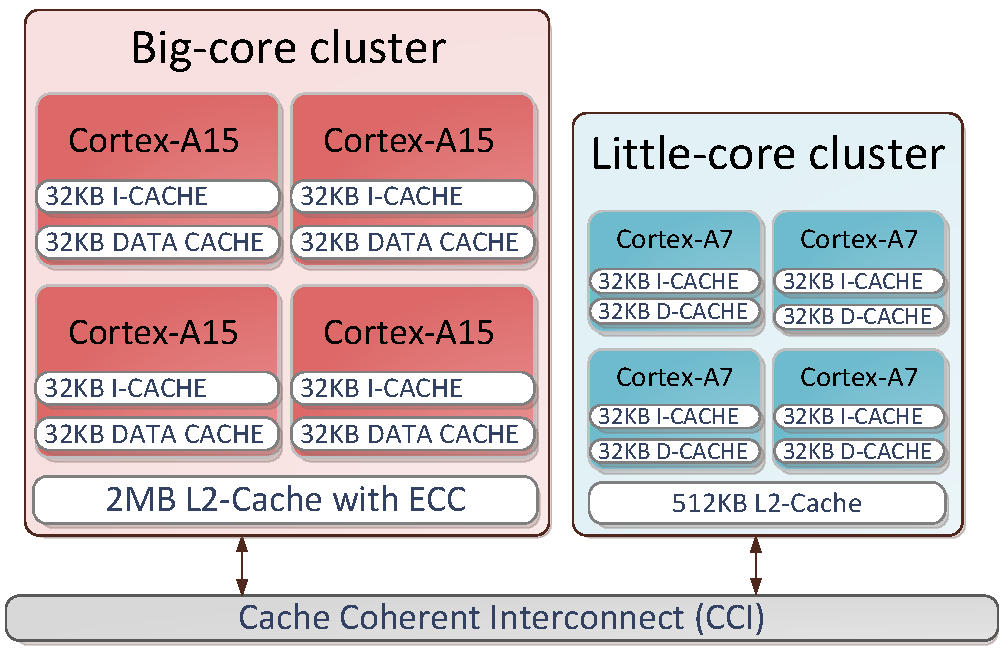
\includegraphics[width=\columnwidth]{figures/block_diagram.pdf}%
        \caption{Samsung Exynos 5422 processor with ARM big.LITTLE architecture.}%
        \label{fig:big-little-diagram}%
        \vspace{-0.56cm}
\end{figure}

In this thesis, we use of one of the commercially available development boards featuring a big.LITTLE architecture: the Hardkernel Odroid-XU3 development board. As shown in Figure~\ref{fig:big-little-diagram}, the Odroid-XU3 includes an 8-core Samsung Exynos 5422 chip with four ARM Cortex-A15 cores and four Cortex-A7 cores. The four Cortex-A15 share a 2~MB 16-way 64-byte-cache-line L2 cache, while the Cortex-A7 cores share a 512~KB L2 cache. A single memory controller provides access to 2~GB of LPDDR3 RAM with dual 32-bit channels at 1866~MT/s. The reason we use this platform instead of the more up-to-date Juno platform~\cite{Juno} is that even if the latter features the more advanced Cortex~A53 and Cortex~A57 cores, it is limited to six cores instead of the 8 cores in Odroid-XU3.


%Odroid gives us the opportunity to evaluate up to eight cores while Juno, even if it features the more advanced Cortex~A53 and Cortex~A57 cores, is limited to only six total cores. 

The Cortex-A7 cores in this SoC support dual-issue of instructions and their pipeline length is between 8 and 10 stages. The L1 instruction cache is 32KB two-way set associative, with virtually indexed and physically tagged cache-lines that can hold up to 8 instructions. The core supports instruction prefetch by predicting the outcome of branches; the prefetch unit can fetch up to a maximum of four instructions per cycle. The L1 data cache is four-way set associative with physically-indexed and physically-tagged cache lines and uses a pseudo-random replacement policy \cite{TRM_A7}. Dynamic Voltage and Frequency Scaling (DVFS) techniques adjust the frequency of the little cores from 200MHz up to 1.4GHz.

The Cortex-A15 cores in this SoC support triple-issue of instructions and their pipeline length is 
between 15 and 24 stages~\cite{MPR_A15}. The L1 instruction and data caches of the Cortex-A15 are 
both 32~KB and 2-way set-associative with 64~byte cache lines. The processor supports speculative 
instruction execution by maintaining a 2-level global history-based dynamic predictor 
with a branch target buffer~\cite{TRM_A15}. The instruction decode unit performs register renaming 
to remove the Write-After-Write and the Write-After-Read hazards, and promote 
instruction reordering~\cite{TRM_A15}. The instruction dispatch unit analyzes instruction dependences 
before issuing them for execution.  The integer execute unit includes 2 
Arithmetic Logical Units with support for operand forwarding. DVFS techniques vary the 
frequency of the big cores from 200~MHz up to 2~GHz.
For the rest of the thesis, we refer to Cortex-A15 cores as \textit{big} and to Cortex-A7 cores as \textit{little}.

All the real machine experiments in this thesis are performed on the Hardkernel Odroid XU3 that features the ARM big.LITTLE architecture. 
To avoid machine overheating, we make use of the \texttt{cpufreq} driver to set big cores at 1.6GHz and little cores at 800MHz. 

%\mm{Explain different pipelines.} \mm{Number of execution units per pipeline?} \mm{ROB size? Maximim number of in-flight instructions?}.  As in the little cores, the data and instruction L1 caches are 32KB each. \mm{FLOPS single and double precision?}.

%In the big.LITTLE processor, the four Cortex-A15 cores form a \emph{cluster} with a shared L2 cache (16-way set-associative with 64 bytes line size), while the Cortex-A7 form a second cluster with a smaller shared L2 cache (8-way 64 bytes cache-line size). This asymmetric multi-core implements the ARMv7 instruction set architecture on all the cores. The two clusters are coherent, so a single shared memory application can run on both clusters, using up to eight cores simultaneously. For the cluster-to-cluster communication, the processor features a cache coherent interconnect. This mechanism allows big and little cores to exchange data at low cost as if they were effectively in the same cluster. Figure~\ref{fig:big-little-diagram} shows a block diagram of such processor.




%%%%%%%%%%%%%%%%%%%
%%%%%%%%%%%%%%%%%%%
% \subsection{Challenges in Scheduling}
% 
% Scheduling a set of processes on an asymmetric multi-core system with big.LITTLE architecture is trickier than the traditional process scheduling on homogeneous multi-cores. 
% An efficient OS scheduler has to take into account the different characteristics of the core types of the system.
% ARM supports two different approaches on scheduling chips with big.LITTLE architecture: the \textit{cluster switching}, and the \textit{global task scheduling}. In this paper we evaluate a different approach which is the \textit{dynamic runtime scheduling} and is not currently used by industry for scheduling such systems. The following subsections describe these different approaches.
% 
% \subsubsection{Cluster Switching}
% In the cluster switching (CS) approach the cores are grouped into two clusters:
% the big-core cluster, that consists of the Cortex-A15 cores of the system and the 
% little-core cluster that consists of the Cortex-A7 cores. 
% At each given time, only one of the clusters is activated; the activated cluster is the one responsible for the execution of the tasks. 
% Thus, the linux OS scheduler does not require any modification and is operating on 4 homogeneous cores each time namely, 
% the cores of the current activated cluster.
% %The deactivated cluster is not processing any task.
% The entire workload of tasks is being managed as a unique entity and the operating system is keeping track of its operational intensity. 
% If the workload reaches a pre-defined threshold, then the entire workload is moved to the other cluster, 
% and the current cluster gets deactivated. 
% %So, the entire workload of tasks is being managed as a unique entity and according to 
% %its operational intensity the OS chooses the appropriate cluster for execution.
% The cluster switching is performed by the CPU frequency framework.
% 
% \subsubsection{Global Task Scheduling (GTS)}
% The second approach is the one that we evaluate in this paper. 
% With the global task scheduling (GTS), all cores are available and visible to the OS scheduler. 
% The OS scheduler is aware of the characteristics and the type of each one of the cores. 
% Moreover, the workload is being managed as a set of tasks, which are practically threads. 
% Each task is characterized by its intensity.
% The OS linux scheduler is modified so that it schedules the high intensity tasks to the big cores (A15 cores)
% and the low intensity tasks to the little cores (A7 cores). 
% This way, the activated cores are chosen according to the tasks of the workload. 
% This is characterized as the most sophisticated method of scheduling tasks on big.LITTLE \cite{samsung}.
% 
% The key benefits of GTS over CS are:
% \begin{itemize}
%  \item Tasks are directly migrated to cores instead of workload being migrated to clusters. This makes the scheduling more flexible and helps on the more effective utilization of the system according to the workload.
% % \item Finer grained control of workloads that are migrated between cores. Because the scheduler is directly migrating tasks between cores, kernel overhead is reduced and power savings can be correspondingly increased.
%  \item Implementation in the scheduler also makes switching decisions faster than in the cpufreq framework, and ARM have reported around 10\% improvements in performance/watt over CS on a range of benchmarks. Samsung reported 20\% improvement in performance.
%  \item GTS can easily support non-symmetrical SoCs (e.g. with 2 Cortex-A15 cores and 4 Cortex-A7 cores)
%  \item The ability to use all cores simultaneously to provide improved peak performance throughput of the SoC compared to CS.
% \end{itemize}
% 
% 
% 
% %Also, interesting slides: http://events.linuxfoundation.org/ sites/events/files/slides/GTS\_Anderson.pdf
% 
% %%%%%%%%%%%%%%%%%%%%%%%%%%%%%%%%%%%%%%%%%%
% %%%%%%%%%%%%%%%%%%%%%%%%%%%%%%%%%%%%%%%%%%
% 
% \subsubsection{Dynamic Scheduling at Runtime Level (task-based)}
% The use of parallel programming models on such systems could increase performance and energy efficiency.
% The increased task granularity that the runtime system can offer has a positive effect on their most effective execution with the minimum possible energy consumption.
% To evaluate this approach we use the OmpSs programming model.
% 
% \textit{OmpSs Programming Model:  }
% OmpSs~\cite{OmpSs} is a task-based programming model conceived as a forerunner of OpenMP. 
% While both OmpSs and OpenMP 4.0 allow the programmers to express tasks and data-dependences between them, OmpSs provides some extra feaatures like runtime support for NUMA-aware allocation or task priorities. 
% OmpSs conceives the parallel execution as a graph where the nodes are sequential pieces of code, the tasks, and the edges are control or data dependences between them.
% 
% The OmpSs runtime is Nanos++, which provides device support for heterogeneity and includes different plug-ins for implementations of scheduling policies, throttling policies, thread barriers, dependency tracking mechanisms, work-sharing and instrumentation. 
% This design allows to maintain the runtime features by adding or removing plug-ins. Thus, the implementation of a new scheduler, or the support of a new architecture becomes simple.
% The implementations of the different scheduling policies in Nanos++ perform various actions on the states of the tasks. A task is \textit{created} if a call to this task is discovered but it is waiting until all its inputs are produced by other previous tasks. When all the input dependencies are satisfied, the task becomes \textit{ready}. The ready tasks of the application at a given point in time are inserted in the \textit{ready queues} as stated by the scheduling policy. Ready queues can be thread-private or shared among multiple threads. When a thread becomes idle, the scheduling policy picks a task from the ready queues for that thread to execute. 
% 
% %\kc{Adding description of fifo scheduler:}
% The default OmpSs scheduling policy is processing the tasks in a first-come first-served manner (FIFO). 
% It maintains a single ready FIFO queue shared among threads for keeping the ready tasks. 
% Whenever a task becomes ready it is pushed to the tail of the ready queue;
% the first available processor, pops the ready task that resides at the head of the ready queue. 
% Simultaneous pushes and pops are protected by the OmpSs locking mechanisms.
% Because the tasks are scheduled dynamically to the available cores, this scheduler achieves automatic load balance without the need of work stealing. 
% Finally, the scheduler is not aware of the task intensity or the core type and its characteristics, but only relies on the availability of tasks and resources.

\iffalse
\mm{Describe only FIFO. In my opinion, extending the evaluation to CATS should be done in an extension paper for a journal.}

Maybe:
\begin{itemize}
 \item Asymmetric Multicores? HW support (Onur Mutlu's ISCAs).
 \item Current processors -- big.LITTLE. Synergistic cores -- Cell.
 \item Other heterogeneous systems: CPU+GPUs, KNL, other accelerators.
\end{itemize}

Hardware support for identifying the most likely critical code segments of parallel applications has been explored. BIC~\cite{Joao:ASPLOS2012} proposes hardware-based tracking of \emph{thread waiting cycles} in parallel regions for bottleneck identification. 
UBA~\cite{Joao:ISCA2013} provides a comprehensive approach for both lagging threads and bottlenecks.


\textbf{Symbiotic cores.}
The ambition of the heterogeneous architecture studies following the nature model of symbiotic relationships
(e.g. water buffalos and birds) is a good approach to optimize overall efficiency of a system. The idea is that
a bunch of less performant cores can take care of a few very performant cores, feeding them with a large
throughput oriented load, minimizing the need to distract their attention to other bookkeeping activities. The
ambition of the project is find out what is the proper dimensioning of such a symbiotic in the development of
highly efficient HPC platforms.

\textbf{From MB3 proposal.}
One of the most widespread approaches to energy efficiency is the use of different computing elements in the
same system. In this task, in particular, we will explore the use of different types of computing cores in an
SoC following a co-design approach between the runtime and architecture. The focus will be on exploring a
symbiotic relationship between small and large cores:

\begin{itemize}
 \item Small cores: Not thought of as the source of computing capacity based on using a large number of
them, but rather seen as support of independent control flows to generate throughput without
perturbing the large/powerful cores, by synchronously executing functions of the runtime that can be
taken out of the critical path and carrying out non-compute bound tasks consuming little power. The
aim is to maximise the efficiency of large cores.

  \item Large cores: Perform bulk of computation task and provide the raw computing power, being
“served” by the small cores. Different variants of the powerful cores will be considered. A first class
of such powerful cores to be considered is the ongoing implementations of the ARM architecture by
multiple companies targeting high performance mobile computing (game-/computer vision-targeted
devices), servers and high capacity systems.

\end{itemize}

We will evaluate different architectural configurations looking at how to integrate large and small cores and
how the runtime can take benefit of such a configuration. We will use the models developed in T5.1 for
conducting actual performance estimation of various architectural configurations. Some of the power models
will also be embedded at this level so as to perform comparative power efficiency assessment of various
configurations.
\fi



\section{The TaskSim Simulator}
\label{sec.background.simulation}
\label{sec.background.simulation}
To evaluate our contributions on larger systems we make use of the TaskSim simulator~\cite{AbstrLevels_TACO12,MUSA}. 
TaskSim is a trace driven simulator, that supports the specification of homogeneous or heterogeneous systems with many cores. 
The tracing overhead of the simulator is less than 10\% and the simulation is accurate as long as there is no contention in the shared memory resources on a real system~\cite{MUSA}.
By default, TaskSim allows the specification of the amount of cores and supports up to two core types in the case of heterogeneous asymmetric systems. 
This is done by specifying the number of cores of each type and their difference in performance between the different types (performance ratio) in the TaskSim configuration file.

Our evaluation consists of experiments on both symmetric and asymmetric platforms with the number of cores varying from 8 to 512.
In the case of asymmetric systems, we simulate the behaviour of an ARM big.LITTLE architecture~\cite{ARM}.


%To set the correct performance ratio between big and little cores, we measure the sequential execution time of each application on a real ARM big.LITTLE platform when running on a little and on a big core. 
%We use the Hardkernel Odroid~XU3 board that includes a Samsung Exynos 5422 chip with ARM big.LITTLE.
%The big cores run at 1.6GHz and the little cores at 800MHz.
%We compare its performance when they run on a little and on a big core.

%% This is TaskGenX specific!!
%Table~\ref{tab.apps} shows the measured performance ratio for each case.
%The average performance ratio among our 13 workloads is 3.8.
%Thus in the specification of the asymmetric systems we use as performance ratio the value 4.

To simulate our approaches using TaskSim we first run each application/input in the TaskSim trace generation mode.
This mode enables the online tracking of task duration and synchronization overheads and stores them in a trace file. 
To perform the simulation, TaskSim uses the information stored in the trace file and executes the application by providing this information to the runtime system.
For our experiments we generate three trace files for each application/input combination on a Genuine Intel 16-core machine running at 2.60GHz.

\section{Task-Based Parallel Programming Models}
\label{sec.background.taskbased}


Parallel programming models ~\cite{Blumofe:PPoPP1995, Reinders2007, Bauer2012, OmpSs},  are widely used to facilitate the programming of parallel codes for multi-core systems.
These programming models offer an abstraction layer to the programer so that multi-threaded programming of an application becomes easier.
They support code annotations that the programmer can add to the application's sequential code and transform it into parallel.
These annotations include the specification of parallel loops, atomic operations, critical regions or task clauses.

Our main focus in this thesis is the task annotation with dependency tracking which OpenMP~\cite{OpenMP} supports since its 4.0 release~\cite{OpenMP4.0:Manual2015}.
A task is a piece of code{\footnote{A piece of code can be a function or a code block.} in the application that can execute simultaneously to other tasks and cooperatively produce results.
In a parallel application there can be many tasks that perform the same computations on different data or tasks that perform different computations on the same data.
By using task annotations, the programmer decomposes the application into tasks and specifies the input and output data dependencies between them.
Parallel programming models typically consist of two parts; a compiler and a runtime system.
The compiler is responsible to parse the code annotations and translate them to code by adding calls to the programming model's runtime system.
The runtime system consists of software threads and is responsible for the efficient execution of the tasks with respect to the data dependencies as well as the availability of resources.
This thesis mainly focuses on enhancements of the runtime system in parallel programming models.

The runtime system creates and manages the software threads for the execution of the tasks. 
Typically one software thread is being bound to each core. 
One of the threads is the \textit{master thread}, and the rest are the \textit{worker threads}. 
The master thread starts executing the compiler generated application's code sequentially and creates the tasks as it encounters them. 
Following task creation, is the analysis of the dependencies of the created task and the insertion of it in the Task Dependency Graph (TDG).

A TDG is a distributed graph structure that connects each task of the application with the rest of the tasks according to their existing input and output data dependencies.
A dependency tracking mechanism is responsible for the maintenance of the input and output data of a task.
Within this mechanism, the runtime system tracks the memory addresses that tasks write or read and according to this, it manages the tasks that are ready for execution\footnote{When the input data of a task is produced, the task can start execution.}.
Tasks that their input data have been produced are marked as \textit{ready} and can start execution, while tasks that are still waiting for input are postponed until their inputs are produced by other executing tasks.

To enable the efficient parallel execution of the tasks, the scheduler of the runtime system keeps track of the available tasks to be executed and manages the task-to-thread allocation.
To do this, the scheduler maintains a \textit{ready queue} and when all of a tasks dependencies are satisfied (i.e., the task becomes \textit{ready}) it is inserted in the \textit{ready queue}. 
All threads have access to this queue which is a first-in-first-out data structure; whenever a thread becomes idle, it pops the next task from the queue and executes it. 
In this thesis we make use of OmpSs~\cite{OmpSs}, a mainstream task-based programming model and the main influence of the updated OpenMP~4.0~\cite{OpenMP}.

\subsection{OmpSs Programming Model}
\label{sec.background.taskbased.ompss}

The OmpSs programming model is a task-based programming model that offers a high level abstraction to the implementation of parallel applications for various homogeneous and heterogeneous architectures~\cite{OmpSs_PPL11,OmpSs}. 
As a task-based programming model, OmpSs enables the annotation of function declarations with the task directive, which declares a task. 
Every invocation of a such function creates a task that is executed concurrently with other tasks or parallel loops. 
OmpSs also supports task dependencies and it uses the StarSs~\cite{StarSs} dependency tracking mechanisms. 
OmpSs is built with the support of the Mercurium compiler, responsible for the translation of the OmpSs annotation clauses to source code, and the Nanos++ runtime system~\cite{nanos}, responsible for the internal creation and execution of the tasks.

As a task-based parallel programming model, OmpSs enables the annotation of function declarations with the task directive. 
If a function is declared as a task, then every invocation of this function creates a task that is executed concurrently with other tasks or parallel loops. 
The accessible data to each task are the arguments of the function. 
OmpSs uses the StarSs~\cite{StarSs} dependency tracking mechanisms and each task may be annotated with the \textit{in}, \textit{out}, \textit{inout} clauses. 
These clauses allow the specification of scalars, arrays and pointers as input, output or input and output data of a task. 
The implementation of a barrier is supported under the \textit{taskwait} clause, and it can also be used with the addition of the \textit{on} clause, to declare a barrier for the group of tasks that produce a specific piece of data. 
These original OmpSs features can now be found in OpenMP 4.0~\cite{OpenMP}.

Nanos++ is an environment designed to serve as the runtime platform of OmpSs. 
It provides device support for heterogeneity and includes different plug-ins for implementations of scheduling policies, throttling policies, thread barriers, dependency tracking mechanisms, work-sharing and instrumentation. 
This design allows to maintain the runtime features by adding or removing plug-ins. 
Thus, the implementation of a new scheduler, or the support of a new architecture becomes simple.

The implementations of the different scheduling policies in Nanos++ perform various actions on the states of the tasks. 
A task is \textit{created} if a call to this task is discovered but it is waiting until all its inputs are produced by other previous tasks. 
When all the input dependencies are satisfied, the task becomes \textit{ready}. 
The ready tasks of the application at a given point in time are inserted in the \textit{ready queues} as stated by the scheduling policy. 
Ready queues can be thread-private or shared among multiple threads. 
When a thread becomes idle, the scheduling policy picks a task from the ready queues for that thread to execute. 

The Nanos++ internal data structures support task prioritization. 
The task priority is an integer field inside the task descriptor that rates the importance of the task. 
If the scheduling policy supports priorities, the ready queues are implemented as \textit{priority queues}. 
In a priority queue, tasks are sorted in a decreasing order of their priority. 
The insertion in a priority queue is always ordered and the removal of a task is always from the head of the queue, i.e., the task with the highest priority. 
The priority of a task can be either set in user code, by using the \textit{priority} clause, which accepts an integer priority value or expression, or dynamically  by the scheduling policy, as is described in the next section.



%%%%% This should be in the TaskGenX Chapter background. It is more specific to this implementation %%%%%%%

%\texttt{Memalloc} is performing the memory allocation for the task and its arguments.
%Next is a runtime call, which is the \texttt{createTask}, responsible for the linking of the task with the runtime system.
%At this point a task is considered \textit{created} and below are the three possible states of a task inside the runtime system:
%\begin{itemize}
%\item \textit{Created:} A task is initialized with the appropriate data and function pointers and it is inserted in the Task Dependency Graph (TDG). The insertion of a task in the TDG implies that the data dependencies of the tasks have been identified and the appropriate data structures have been created and initialized. 
%\item \textit{Ready:} When all the data dependencies of a created task have been satisfied, the task is ready and it is inserted in the \textit{ready queue} where it waits for execution. 
%\item \textit{Finished:} When a task has finished execution and has not been deleted yet.
%\end{itemize}

%Listing~\ref{taskCreation} shows the pseudo-code for the task creation step within the runtime.
%The \texttt{createTask} function is first initializing the task by copying the corresponding data to the allocated memory as well as connecting the task to its parent task (\texttt{initAndSetupTask}).
%After this step, the task is ready to be inserted in the TDG. 
%The TDG is a distributed and dynamic graph structure that the runtime uses to keep the information about the current tasks of the application. 
%The insertion of a task in the TDG is done by the \texttt{insertToTDG} function.
%This function takes as arguments a list with all the memory addresses that are to be written or read by the task (\texttt{dList}), and the task itself.
%Listing~\ref{insertTDG} shows the pseudo-code for the TDG insertion. 
%If for a task the \texttt{dList} is empty (line 2), this means that there are no memory addresses that need to be tracked during the execution; thus, the task is marked as \textit{ready} by pushing it to the \textit{ready queue} (line 3).
%Each entry of \texttt{dList} contains the actual memory address as well as the access type (read, write or read-write).
%The runtime keeps a distributed unified dependency tracking structure, the \texttt{depMap} where it stores all the tracked memory addresses together with their writer and reader tasks.
%For each item in the \texttt{dList} the runtime checks if there is an existing representation inside the \texttt{depMap} (line 8).
%If the memory address of an entry of the \texttt{dList} is not represented in the \texttt{depMap}, it is being added as shown in line 9.
%If the address of a \texttt{dList} item exists in the \texttt{depMap}, this means that a prior task has already referred to this memory location, exhibiting a data dependency.
%According to the access type of \texttt{d}, the readers and the writers of the specific address are updated in the \texttt{depMap} (lines 10-15).
%
%To reduce the lookup into the \texttt{depMap} calls, every time the contents of a memory address are modified, the tasks keep track of their \textit{successors} as well as the number of \textit{predecessors}.
%The \textit{successors} of a task are all the tasks with inputs depending on the output of the current task.
%The \textit{predecessors} of a task are the tasks whose output is used as input for the current task.
%When a \texttt{read} access is identified, the task that is being created is added to the list of successors of the last writer task, as shown on line 20 of Listing~\ref{taskCreation}.
%
%As tasks are executed, the dependencies between them and their successors are satisfied. 
%So the successor tasks that are waiting for input, eventually become \textit{ready} and are inserted to the ready queue.
%When a task goes to the \textit{finished} state, the runtime has to perform some actions in order to prepare the successor tasks for execution.
%These actions are described in Listing~\ref{taskFinish}.
%The runtime first updates the \texttt{depMap} to remove the possible references of the task as reader or writer (line 2).
%Then, if the task does not have any successors, it can safely be deleted (line 3).
%If the task has successors, the runtime traverses the successor list and for each successor task it decreases its predecessor counter (lines 5-6).
%If for a successor task its predecessor counter reaches zero, then this task becomes \textit{ready} and it is inserted in the \textit{ready queue} (lines 7-8).
%\begin{lstlisting}[float, emph={is, void,if,return,Dependency,DepList,Data,Task,not,for,true,and,break}, captionpos=b, caption={Pseudo-code for TDG insertion},label=insertTDG, emph={[2]mat}, emphstyle={[2]}, aboveskip={0\baselineskip}, frame=tb, belowskip={0\baselineskip}]
%void insertToTDG(DepList dList, Task t) {
% if( dList is empty ) {
%   readyQ->push(t);
%   return;
% }
% Dependency entry;
% for( d in dList ) {
%   entry = depMap[d.address()];
%   if(entry==NULL) depMap.add(entry, t);
%   if(d.accessType() == "write")
%     entry.addLastWriter(t);
%   if(d.accessType() == "read") {
%     entry.addReader(t);
%     entry.lastWriter()->addSuccessor(t);
%   }
% }
%}
%\end{lstlisting}
%The runtime activity takes place at the task state changes. 
%One state change corresponds to the task creation, so a task from being just allocated it becomes \textit{created}. 
%At this point the runtime prepares all the appropriate task and dependency tracking data structures as well as inserts the task into the TDG.
%The second change occurs when a task from being \textit{created} it becomes \textit{ready};
%this implies that the input dependencies of this task are satisfied so the runtime schedules and inserts the task into the ready queue.
%The third change occurs when a running task finishes execution. 
%In this case, following our task states, the task from being \textit{ready} it becomes \textit{finished}; this is followed by the runtime updating the dependency tracking data structures and scheduling possible successor tasks that become ready. 
%For the rest of the paper we will refer to the first state change runtime activity as the task creation overheads (\textit{Create}).
%For the runtime activity that takes place for the following two state changes (and includes scheduling and dependence analysis) we will use the term runtime overheads (\textit{Runtime}).

%\subsection{Motivation}
%
%\begin{figure}[t!]%
%	\centering
%	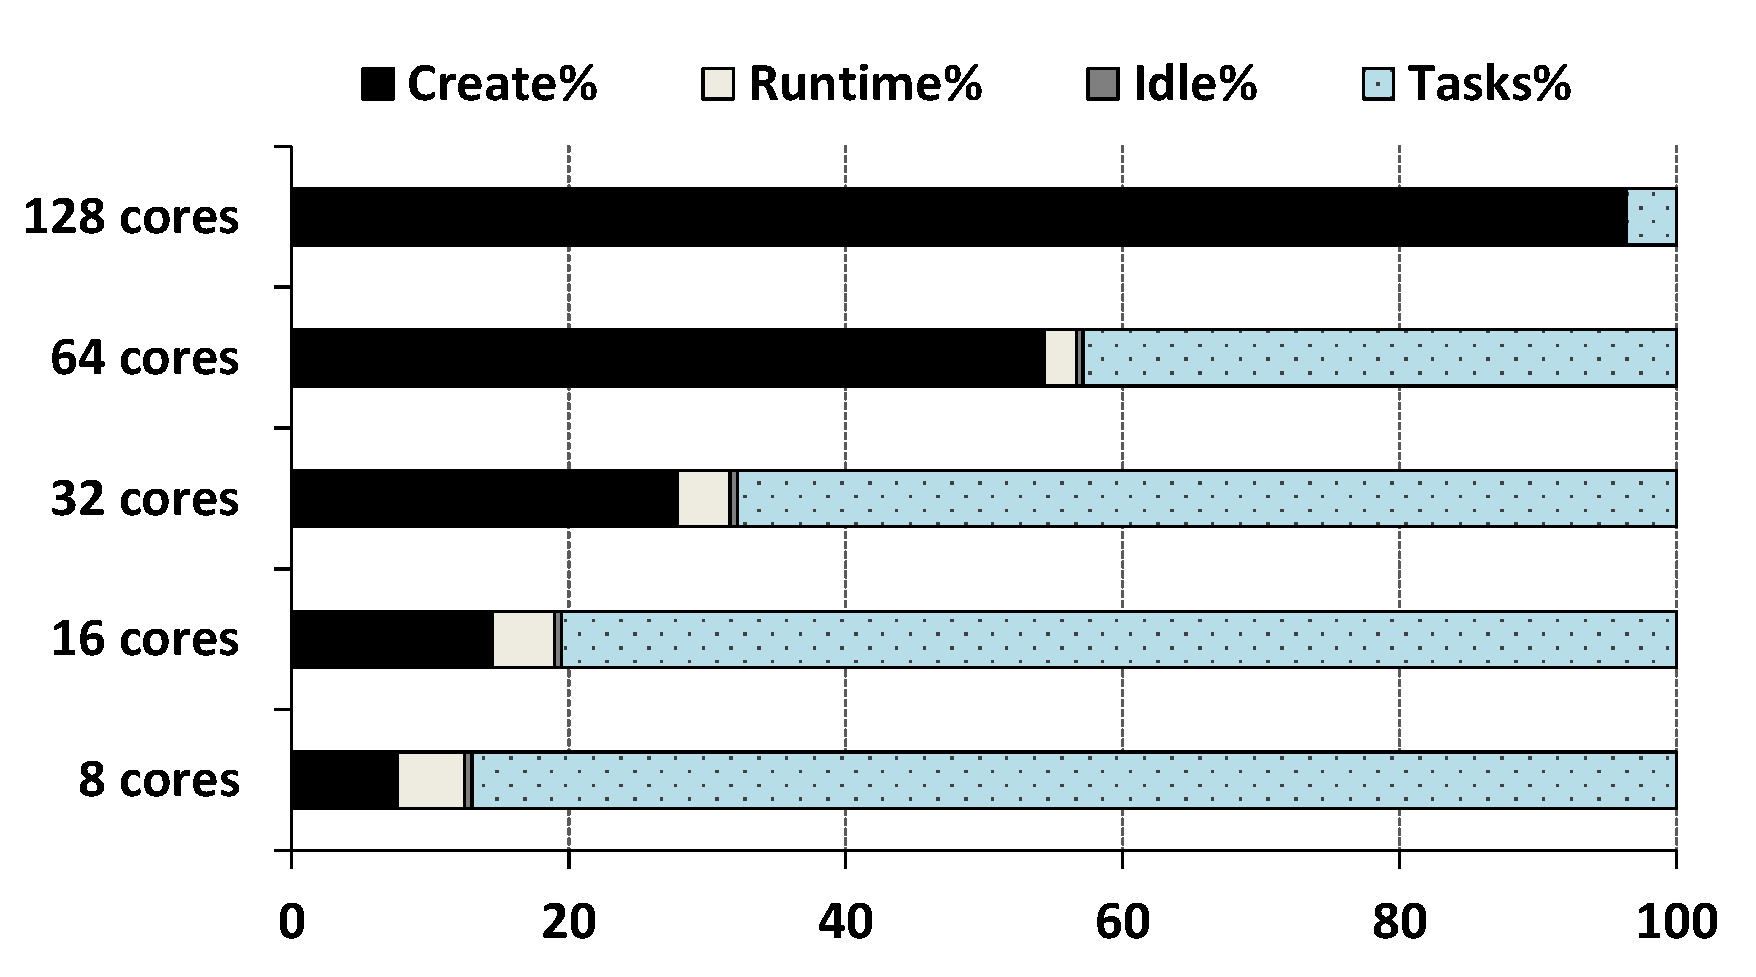
\includegraphics[width=0.75\columnwidth]{figures/master_thread.pdf}
%	\caption{Master thread activity for Cholesky as we increase the number of cores.}
%	%\caption{Performance improvements on a big.LITTLE processor with different $(F,N)$ configurations, where $F$ is the total number of big cores and $N$ the total number of cores. Results are normalized to running on four little cores with pinned Pthreads.}%
%	\label{fig:master_thread}%
%\end{figure}
%
%Figure~\ref{fig:master_thread} shows the runtime activity of the master thread during the execution of the Cholesky{\footnote{Details about the benchmarks used are in Section~\ref{sec:experimental}} benchmark on 8, 16, 32, 64 and 128 cores\footnote{The experimental set-up is explained in Section~\ref{sec:experimental}}.
%The execution time represented here is the wall clock time during the parallel region of the benchmark.
%Each one of the series represents a different runtime overhead from the ones described above.
%%\textit{Create} represents the \textit{Creation} step, 
%%\textit{Runtime} refers to the \textit{Finish} step, \textit{Idle} shows the master thread's idle time and the \textit{Tasks} is the time spent on task execution. 
%The percentage of time spent on task creation is increasing as we increase the number of cores.
%This is because the creation overhead is invariant of core count: the more we reduce the application's execution time by adding resources the more important this step becomes in terms of execution time.
%In contrast, the task execution time percentage is decreased as we increase the number of cores because the computational activity is being shared among more resources.
%One way to reduce the task creation overhead is by introducing nested parallelism. 
%In this programming technique, every worker thread is able to generate tasks thus the task creation is spread among cores and its overhead is reduced.
%However, not all applications can be implemented with this parallelization technique and there are very few applications using this scheme.
%\textit{Runtime} decreases as we increase the number of cores because this activity is also shared among the resources.
%This is because this part of the runtime takes place once the tasks finish execution and new tasks are being scheduled. 
%So the more the resources, the less the runtime activity per thread, therefore less activity for the master thread.
%%\kc{explain that this is wall clock time. The \textit{Runtime} activity is actually the part of the master thread but also the worker threads are performing this activity while the Create is only within the master thread.}
%
%\begin{lstlisting}[float, emph={void,if,return,Task,for,not,true,and,break}, captionpos=b, caption={Pseudo-code for task$\_$finish runtime activity.},label=taskFinish, emph={[2]mat}, emphstyle={[5]}, aboveskip={0\baselineskip}, frame=tb, belowskip={0\baselineskip}]
%void task_finish(Task *t) {
%  depMap.removeReaderWriter(t);
%  if(t->successors.empty()) delete t;
%  else {
%    for( succ in t->successors ) {
%      succ.decreasePredecessors();
%      if(succ.numPredecessors == 0) 
%        readyQ->push(succ);
%    }
%  }
%}
%\end{lstlisting}
%
%Our motivation for this work is the bottleneck introduced by task creation as shown in Figure~\ref{fig:master_thread}.
%Our runtime proposal decouples this piece of the runtime and accelerates it on a specialized hardware resulting in higher performance.
%


\section{Applications}
\label{sec.background.applications}
%applications
In the evaluation of our contributions we use 13 scientific applications. 
With the prevalence of many-core processors and the increasing relevance of application 
domains that do not belong to the traditional HPC field, comes the need for programs 
representative of current and future parallel workloads. 
The PARSEC benchmark suite~\cite{PARSEC3,Bienia:PhD2011} features state-of-the-art, 
computationally intensive algorithms and very diverse workloads from different areas of computing.
In our experiments, we make use of the original PARSEC codes together with a task-based 
implementation of nine benchmarks of the suite~\cite{Chasapis:TACO2016}. 
Additionaly, we evaluate some representative benchmarks from the BSC Application Repository (BAR)~\cite{BAR}.
These applications are implemented using the OmpSs programming model.

Table~\ref{tab:parsec} describes the benchmarks included in the study along with their respective 
inputs and parallelization strategy. 
We are using native inputs, which are real input sets for native execution, except for \texttt{dedup}, as the entire input file of 672 MB and the intermediate data structures do not fit in the memory system of our platform. 
Instead, we reduce the size of the input file to 351 MB.

%We obtain these applications from the PARSECSs benchmark suite~\cite{Chasapis:TACO2016} as well as from the BSC Application Repository (BAR)~\cite{BAR}.
%These applications are implemented using the OmpSs programming model and/or the pthreads library.
%In our evaluations we either compare our contributions against the default OmpSs runtime or we compare the OmpSs runtime against the application-level (pthreads version) parallelism.
%Table~\ref{tab.apps} shows the applications together with a short description and the parallelization strategy followed in their task-based implementation.
%In the next Chapters, depending on the present evaluation we will update this Table with the appropriate information to facilitate the explanation of the results.


\begin{table*}[h]
	\centering
	\scriptsize
	\caption{Benchmarks used from the PARSEC benchmark suite and their measured performance ratio between big and little cores}
    %\vspace{-0.2cm}
	\setlength{\tabcolsep}{3pt}
	\begin{tabular}{|p{2cm}|p{5.7cm}|p{4.5cm}|c|}
	\hline
	\textbf{Benchmark} & \multicolumn{1}{|c|}{\textbf{Description}} & \multicolumn{1}{|c|}{\textbf{Input}} & \textbf{Parallelization} \\
	\hline \hline
	Blackscholes & Calculates the prices of a portfolio analytically with the Black-Scholes partial differential equation. & 10,000,000 options & data-parallel \\ \hline
	Bodytrack & Computer vision application which tracks a 3D pose of a marker-less human body with multiple cameras through an image sequence. & 4 cameras, 261 frames, 4,000 particles, 5 annealing layers & pipeline\\ \hline
	Canneal & Simulated cache-aware annealing to optimize routing cost of a chip design. & 2.5 million elements, 6,000 steps & unstructured\\ \hline
	Cholesky Factorization & Dense matrix operation that is used for solving linear equations in linear least square systems. & \kc{multiple} & dependencies\\ \hline
	Dedup & Compresses a data stream with a combination of global compression and local compression in order to achieve high compression ratios. & 351 MB data & pipeline\\ \hline
	Facesim & Takes a model of a human face and a time sequence of muscle activation and computes a visually realistic animation of the modeled face. & 100 frames, 372,126 tetrahedra & data-parallel\\ \hline
	Ferret & Content-based similarity search of feature-rich data (audio, images, video, etc.) & 3,500 queries, 59,695 images database, find top 50 images & pipeline\\ \hline
	Fluidanimate & Extended Smoothed Particle Hydrodynamics method to simulate an 
incompressible fluid for interactive animations. & 500 frames, 500,000 particles & 
data-parallel\\ \hline
	Heat diffusion & Computes the heat distribution on a matrix from \textit{x} heat sources using the Gaus-Seidel method. & 16$\times$16 blocks of 512$\times$512 doubles & data-parallel\\ \hline
	Integral Histogram & A method to compute a cumulative histogram for each pixel of an image represented as a Cartesian data space in constant time. & 8$\times$8 blocks of 12$\times$512 floats & dependencies \\ \hline
	QR Factorization & A linear algebra algorithm that is used to solve the linear least squares problem \cite{QR}.& \kc{multiple} & dependencies \\ \hline
	Streamcluster & Solves the online clustering problem. & 200K points per block, 5 block & 
data-parallel\\ \hline
	Swaptions & Intel RMS workload; uses the Heath-Jarrow-Morton framework to price a portfolio of swaptions. & 128 swaptions, 1 million  simulations & data-parallel\\ \hline
%	vips & VASARI Image Processing System (VIPS), which includes fundamental image processing operations. & 18,000$\times$18,000 pixels & 127,957\\ \hline
%	x264 & H.264/AVC (Advanced Video Coding) video encoder. & 512 frames, 1,920$\times$1,080 pixels & 29,329\\ \hline 
	\end{tabular}
	\label{tab:parsec}
	%\vspace{-0.3cm}
\end{table*}



%\chapter{Study of Asymmetric Systems}
\chapter{Study of Asymmetric Systems}

%%%%%%%%%%%%%%%%%%%
%%%%%%%%%%%%%%%%%%%
\section{Introduction}
\label{sec:intro}

%%%%%%%%%%%%%%%%%%%%%%%%%%%
%%%%%%%%%%%%%%%%%%%%%%%%%%%
% \mm{Idea for the Introduction}
% 
% Heterogeneous multicores are a reality in the mobile world.
% 
% Systems composed of big and little cores can switch from low power to high responding operation modes.
% 
% Many researchers are pushing towards building future desktop and HPC systems with mobile chips.
% 
% In this paper, we explore the maturity of these platforms for parallel desktop applications, as well as of the programming models used to program them.

%The conventional wisdom in the high-performance computing (HPC) community predicts the power budget of the first exaFLOPS machines to be of a few tens of megawatts~\cite{Kogge_Exascale_TR08}. Should this prediction be correct, the energy efficiency of such machine needs to be around 20-30 times higher than that of the top supercomputers today. This makes energy efficiency, among others such as reliability, storage and networking, one of the main issues for the design of exascale computing technology.

%Using heterogeneous processing elements is one of the approaches to increase energy efficiency. Different types of processors can be specialized for different types of computation, such as the combination of chip-multiprocessors (CMP) and discrete compute-capable graphics processing units (GPUs). Another approach towards heterogeneity is the use of different processors designed targeting different performance and power optimization points, such as the combination of faster and slower cores in a CMP (e.g., ARM big.LITTLE~\cite{Greenhalgh2011}).


%Heterogeneity in supercomputing nowadays comes mainly from the use of compute accelerators. Generally, general-purpose chip multiprocessors (CMPs) made out of homogeneous cores are combined together with compute-capable graphics processing units (GPUs) that serve as accelerators for compute-intensive parts of an application. This provides a platform in which some parts of the application will run faster on the CMP, and others on the GPU.

%The STI Cell/B.E.~\cite{IntroCell_IBMRandD05} has been one of the major processors with heterogeneous processing elements on the same chip. It was targeted to the gaming market and its compute capabilities attracted HPC users and vendors. It was substantially adopted in supercomputing and was the most energy efficient HPC technology for some years before being discontinued and becoming obsolete. There are no other recent examples of heterogeneous CMPs used in supercomputing. However, heterogeneous CMPs are mainstream in embedded multimedia and mobile processing. Apart from the processor-accelerator scheme using VLIW/DSP cores~\cite{Viper_IEEEDandT01} or GPUs, some heterogeneous CMPs integrate different types of general-purpose cores~\cite{Greenhalgh2011}. Some works envision the adoption of such mobile technology in HPC for energy efficiency~\cite{ARM4HPC_SC13,Abdurachmanov2013}. In this scenario, a heterogeneous CMP with general-purpose fast and slow cores imposes several challenges regarding scheduling that are different to the current accelerator-based heterogeneous systems. Contrarily to the latter, different parts of an HPC application will constantly run faster on fast cores and slower on slow cores.

%Using heterogeneous processing elements is one of the approaches to increase energy efficiency~\cite{Fedorova2009}. Different types of processors can be specialized for different types of computation, such as the combination of chip-multiprocessors (CMP) and discrete compute-capable graphics processing units (GPUs). Another approach towards heterogeneity is the use of different processors designed targeting different performance and power optimization points, such as the combination of faster and slower cores in a CMP (e.g., ARM big.LITTLE~\cite{Greenhalgh2011}).

% <ISPASS17>
The future of parallel computing is highly restricted by energy efficiency~\cite{Kogge_Exascale_TR08}. 
Energy efficiency has become the main challenge for future processor designs, motivating prolific research to face the \emph{power wall}. 
Using heterogeneous processing elements is one of the approaches to increase energy efficiency~\cite{CompCores,hetServers}. 
%Different types of processors can be specialized for different types of computation, such as the combination of general-purpose cores with accelerators such as Graphics Processing Units (GPUs). 
%Another approach towards heterogeneity is the use of asymmetric multi-cores (AMCs).
%An interesting approach towards energy efficiency is the use of asymmetric multi-core (AMC) systems.
Asymmetric multi-core (AMC) systems is an interesting case of heterogeneous systems to utilize for energy efficiency.
These systems maintain different types of cores that support the same instruction-set architecture. 
The different core types are designed to target different (performance or power) optimization points~\cite{Kumar:ISCA2004,Balakrishnan:ISCA2005,Pangaea}. 

AMCs have been mainly deployed for the mobile market. 
Mobile processors are also utilized in HPC platforms aiming to energy savings~\cite{ARMV8}.
Asymmetric mobile SoCs combine low-power simple cores (\emph{little}) with fast out-of-order cores (\emph{big}) to achieve high performance while keeping power dissipation low.
Another area where AMCs have been successful is the supercomputing market.
The Sunway TaihuLight supercomputer topped the Top500 list in 2016 using AMCs. 
In this setup, big cores, that offer support for speculation to exploit Instruction-Level Parallelism (ILP), run the master tasks such as the OS and runtime system.
Little cores are equipped with wide Single Instruction Multiple Data (SIMD) units and lean pipeline structures for energy efficient execution of compute-intensive code. 

%Previous experiences have shown that load balancing and scheduling are fundamental challenges that must be addressed to effectively exploit all the resources in these platforms~\cite{Suleman:APLOS2009,Fedorova2009,Greenhalgh2011,Joao:ASPLOS2012,Joao:ISCA2013,ARM4HPC_SC13}. 
Like in other heterogeneous systems, load balancing and scheduling are fundamental challenges that must be addressed to effectively exploit all the resources in AMC platforms~\cite{Suleman:APLOS2009,Fedorova2009,Greenhalgh2011,Joao:ASPLOS2012,Joao:ISCA2013,ARM4HPC_SC13}. 
Mobile applications rely on multi-programmed workloads to balance the load in the system, while supercomputer applications rely on hand-tuned code to extract maximum performance. 
However, these approaches are not always suitable for general-purpose parallel applications.

In this paper, we evaluate several execution models on an AMC using the PARSEC benchmark suite~\cite{PARSEC3}. 
This suite includes parallel applications from multiple domains such as finance, computer vision, physics, image processing and video encoding. 
We quantify the performance loss of executing the applications \textit{as-is} on all cores in the system. 
These applications were developed on homogeneous platforms and are bound to suffer from load imbalance on parallel regions that statically distribute the work evenly across cores without considering their performance disparity.

To overcome this matter, we consider two possible solutions at the OS and runtime levels to exploit AMCs effectively.
The first solution delegates scheduling to the OS.
We evaluate the built-in heterogeneity-aware OS scheduler currently used in existing mobile platforms that automatically assigns threads to different core types based on CPU utilization. 
%This approach does not require modifying the application, but is limited for high-utilization multithreaded applications.

The second solution is to transfer the responsibility to the runtime system so it dynamically schedules work to different core types based on work progress and core availability. 
%The advantage is that the runtime system has knowledge of the application structure and parallel work boundaries so it can react with certain level of predictability. 
We evaluate the impact of using an inherently load-balanced execution model such that of task-based programming models. 
Recent examples~\cite{Ayguade:TPDS2009, OpenMP4.0:Manual2013, OmpSs_PPL11, vectorMulticore, Bauer.2012.SC,rollback,Vandierendonck:PACT2011, Vandierendonck:Hyperq,spawn} include clauses to specify inter-task dependencies and remove most barriers which are the major source of load imbalance on AMCs.
Another approach of scheduling in the runtime system is to change the existing statically-scheduled work-sharing constructs for the applications implemented in OpenMP to use dynamic scheduling. 

This paper provides the first to our knowledge comprehensive evaluation of representative parallel applications on a real AMC platform: the Odroid-XU3 development board with ARM big.LITTLE architecture.
We analyze the effectiveness of the aforementioned scheduling solutions in terms of performance, power and energy.
We show why parallel applications are not ready to run on AMCs and how OS and runtime schedulers can overcome these issues depending on the application characteristics.
Further we point out in which aspects the built-in OS scheduler falls short to effectively utilize the AMC.
Finally, we show how the runtime system approach overcomes these issues, and improves the OS and static threading approaches by 13\% and 23\% respectively.

%that the commonly used OS scheduler for AMCs 
%how a runtime-based approach outperforms a commercially available product 

% the effectiveness of these solutions at different levels of the software stack with a comprehensive evaluation of representative parallel applications on a real AMC platform: the Odroid-XU3 development board. 
%This platform features an eight-core Samsung Exynos 5422 chip with ARM big.LITTLE architecture with four out-of-order Cortex-A15 and four in-order Cortex-A7 cores.

The rest of this document is organized as follows: Section~\ref{sec:background} describes the evaluated AMC processor, while Section~\ref{sec:scheduling} provides information on 
scheduling at the OS and runtime system levels. 
Section~\ref{sec:experimental} describes the experimental framework. 
Section~\ref{sec:evaluation} shows the performance and energy results and associated insights.% of our experiments. 
Finally, Section~\ref{sec:related} discusses related work and Section~\ref{sec:conclusions} concludes this work. 

\iffalse
% <PACT16>

The future of parallel computing is highly restricted by energy 
efficiency~\cite{Kogge_Exascale_TR08}. Energy efficiency has become the main 
challenge for future processor designs, motivating prolific research to face the 
\emph{power wall}. Using heterogeneous processing elements is one of the 
approaches to increase energy efficiency. Different types of processors can 
be specialized for different types of computation, such as the combination of 
general-purpose cores with accelerators such as Graphics Processing Units (GPUs). 
Another approach towards heterogeneity is the use of asymmetric multi-cores 
with different types of cores with the same instruction-set architecture. Different core types 
target different performance and power optimization points for energy
efficiency~\cite{Kumar:ISCA2004,Balakrishnan:ISCA2005}. 

Asymmetric multi-cores have been successfully deployed in the mobile market, where 
low-power simple cores (\emph{little}) are combined with 
high-performance out-of-order cores (\emph{big}). Low demand applications
run on little cores for low power operation and prolong battery life. Demanding
applications, such as games, run on the big cores providing high performance
when needed.

Supercomputing is another market where asymmetric multi-cores have been successful. 
The Sunway TaihuLight supercomputer topped the Top500 list in 2016 using asymmetric multi-cores. 
In this setup, big cores, that offer support for speculation and Instruction-Level Parallelism (ILP), run the master tasks such as the OS and runtime system.
%system, as these tasks require support for speculation and Instruction-Level Parallelism (ILP) 
%exploitation of codes with complex control flow.
Little cores are equipped with wide Single Instruction Multiple Data (SIMD) units and lean pipeline structures for energy efficient execution of compute-intensive codes. 

Previous experiences have shown that load balancing and scheduling are fundamental challenges that 
must be addressed to effectively exploit all the resources in these 
platforms~\cite{Suleman:APLOS2009,Fedorova2009,Greenhalgh2011,Joao:ASPLOS2012,Joao:ISCA2013,
ARM4HPC_SC13}. 
Mobile applications rely on multi-programmed workloads to balance the load in the 
system, while supercomputer applications rely on hand-tuned code to extract maximum 
performance. However, these approaches are not always suitable for general-purpose parallel 
applications.
%In a first generation of asymmetric multi-cores, the system could switch from low power to high responding operation modes, activating or de-activating the cluster of big or little cores accordingly~\cite{ARM}. In a second generation of asymmetric multi-core processors, all the cores can run simultaneously to further improve the peak performance of these systems~\cite{samsung}.

%Many researchers are pushing towards building future parallel systems with asymmetric multi-cores~\cite{Suleman:APLOS2009,Fedorova2009, Greenhalgh2011, Joao:ASPLOS2012,Joao:ISCA2013} and even mobile chips~\cite{ARM4HPC_SC13}. However, it is unclear if current parallel applications will benefit from these asymmetric platforms. Load balancing and scheduling are two of the main challenges in utilizing such heterogeneous platforms, as the programmer has to consider them from the very beginning to obtain an efficient parallelization.

%In this paper, we evaluate for the first time the suitability of currently available mobile asymmetric multi-core platforms for general purpose computing. First, we demonstrate that out-of-the-box parallel applications do not run efficiently on asymmetric multi-cores. Fully exploiting the computational power of these processors is challenging as the asymmetry in the system can lead to load imbalance, undermining the scalability of the parallel application. Consequently, only applications that incorporate user-defined load balancing mechanisms can benefit immediately from asymmetric multi-cores.

In this paper, we evaluate several execution models on an asymmetric multi-core
using the PARSEC benchmark suite. This suite includes parallel applications from multiple domains 
such as finance, computer vision, physics, image processing and video encoding. We first quantify 
the performance loss of executing the applications \textit{as-is} on all cores 
in the system. These applications were developed on homogeneous platforms and are bound to suffer from
load imbalance on parallel regions that statically distribute the work
evenly across cores without considering their performance disparity.

Then, we evaluate several solutions at the OS and runtime level that require different
levels of user intervention to exploit asymmetric multi-cores effectively. The first
solution delegates scheduling to the OS. We evaluate the heterogeneity-aware
OS scheduler used in existing mobile platforms that assigns threads to different
core types based on CPU utilization. This requires no modification of the
application, but has limited capability for high-utilization multithreaded applications.

%on an ARM big.LITTLE asymmetric multi-core platform 

%When load-balancing techniques are not included in the original application, we evaluate alternative solutions that, without relying on the programmer, can leverage the opportunities that asymmetric systems offer. In particular, we evaluate a state of the art dynamic scheduler at the Operating System (OS) level that is aware of the characteristics of each core type. This scheduler effectively exploits the system by running high CPU utilization processes on the big cores and low CPU utilization processes on the little cores.

The second solution is to transfer the responsibility to the runtime system so it 
dynamically schedules work to different core types based on work progress and core 
availability. The advantage is that the runtime system has knowledge of the application 
structure and parallel work boundaries so it can react with certain level of predictability. 
We evaluate dynamic scheduling on top of the existing work-sharing constructs in the applications 
with an OpenMP statically-scheduled implementation available. This requires code transformations 
that are straightforward in many cases.

Finally, we evaluate the impact of using an inherently load-balanced execution model such 
that of task-based programming models. 
Recent examples~\cite{Ayguade:TPDS2009, OpenMP4.0:Manual2013, OmpSs_PPL11, Zuckerman:EXADAPT2011, Bauer.2012.SC, Vandierendonck:PACT2011, Vandierendonck:Hyperq} 
include clauses to specify inter-task dependences and remove most barriers which are the major 
source of load imbalance on asymmetric multi-cores.

%and let the runtime system to track dependences between tasks. When these dependences are satisfied, tasks are dynamically scheduled, effectively balancing the workload.

This paper quantifies the effectiveness of these solutions at different levels of the software stack
with a comprehensive evaluation of representative parallel applications on a real 
asymmetric multi-core platform: the Odroid-XU3 development board. This platform features an 
eight-core Samsung Exynos 5422 chip with ARM big.LITTLE architecture with 
four out-of-order Cortex-A15 and four in-order Cortex-A7 cores.

The rest of this document is organized as follows: Section~\ref{sec:background} describes the 
evaluated asymmetric multi-core processor, while Section~\ref{sec:scheduling} offers information on 
dynamic schedulers at the OS and runtime system levels. Section~\ref{sec:experimental} 
describes the experimental framework. Section~\ref{sec:evaluation} shows the performance 
and energy results and associated insights of our experiments. Finally, 
Section~\ref{sec:related} discusses related work and Section~\ref{sec:conclusions} concludes 
this work. 
\fi
%\begin{itemize}
% \item Out-of-the-box applications obtain the best average performance when running only on the aggressive out-of-order cores. Many of these applications are not ready to fully exploit asymmetric multi-cores as they suffer from load imbalance due to the system's heterogeneity. As a result, an average 12\% performance degradation is obtained when using all the cores in the system instead of the four out-of-order cores. 
% \item For the OS scheduler it takes three additional little cores on average to reach the performance obtained with four out-of-order cores. This is observed in most evaluated applications; the addition of little cores to a homogeneous big-core system is degrading performance. Specifically, this slowdown is observed to be 22\% on average when one little core is added to a system that consists of four big cores.
%% applications have 22\% better performance on four big cores compared to their performance on a system with four big and one little cores. 
%When adding four little cores the OS scheduler reduces total execution time by 5.3\% but contrarily to this, it is shown how the runtime system scheduling constantly improves performance by up to 16\%.
%  
%% \item Dynamic scheduling techniques at OS level can turn the tables, reducing the total execution time by 5.3\% when adding four little cores to a system with four big cores. The dynamic scheduler in the runtime system can further improve the final performance by fully utilizing all the resources in the system. This approach reaches an average 13\% speedup, and leads to the most energy efficient solution, as the Energy-Delay Product (EDP) is reduced by 40\% in this configuration.
% \item Moreover, the energy delay product (EDP) results show that the optimal solution taking into account both energy and performance remains the runtime system scheduling.
%%  In systems with a given number of out-of-order cores, adding extra in-order cores can further boost the performance of the application with the appropriate software support (at the application, runtime or OS level). As a result, the energy consumption of parallel applications running on those systems can be reduced by XXX\% on a system with four in-order and four out-of-order cores.
% \item Finally, we evaluate the usefulness of little cores to off-load runtime system activities. Similarly to the assistant core in the IBM Blue Gene Q and the Fujitsu SPARC64 XIfx processors~\cite{BG-Q:HotChips2011, Fujitsu:HotChips2014}, we explore the possibilities of devoting a little or big core to the runtime system activity. In general, we observe that the noise introduced by the runtime system does not degrade the performance of the parallel application. Thus, we can make use of this assistant core to also run user tasks, increasing the final performance of the system.
%\end{itemize}


% </PACT16>

% We describe a set of configurations for our scheduler regarding the work stealing capabilities of the different core types and the flexibility to define a task as critical or non-critical. 
 
% We implement this scheduler in OmpSs and evaluate its effectiveness on different numbers of cores and shares of fast and slow cores on a real system. 
 
% We also evaluate the effectiveness of our scheduler depending on the speed ratio between fast and slow cores using simulation.  The results show that the effectiveness of our scheduler increases with larger numbers of fast cores over slow cores, and with larger differences of performance between fast and slow cores.

%Finally, we provide a set of recommendations on how to configure our scheduler to get the best results depending on the target system size and configuration.


%%%%%%%%%%%%%%%%%%%
%%%%%%%%%%%%%%%%%%%
\section{Scheduling in Asymmetric Multi-Cores}
\label{sec:scheduling}
%%%%%%%%%%%%%%%%%%%%%%%%%%%%%%%%%%%%%%%%%%
%%%%%%%%%%%%%%%%%%%%%%%%%%%%%%%%%%%%%%%%%%
Scheduling a set of processes on an AMC system is more challenging than the traditional process scheduling on SMCs. 
An efficient OS scheduler has to take into account the different characteristics of the cores and act accordingly~\cite{coolingAware}.
There have been three mainstream OS schedulers for ARM big.LITTLE systems: \textit{cluster switching}, 
\textit{in-kernel switch} and \textit{global task scheduling}, described in the next sections.
In the case of parallel applications, \textit{dynamic scheduling at the runtime system level} can be exploited to balance the workload among the different cores and is described in section~\ref{sec:runtime}.


%%%%%%%%%%%%%%%%%%%%%%%%%%%%%%%%%%%%%%%%%%
\subsection{Cluster Switching and In-Kernel Switch}
%%%%%%%%%%%%%%%%%%%%%%%%%%%%%%%%%%%%%%%%%%
In the Cluster Switching (CS) approach~\cite{samsung}, only one of the clusters is active at any given time: either the cluster with little cores or the cluster with big cores executes. Thus, the OS scheduler operates on a \emph{de-facto} symmetric multi-core with only four cores, namely the cores of the current active cluster. The policy to change the operating cluster is based on CPU utilization. When idle, background processes are executed on the little cores. When CPU utilization surpasses a threshold, all processes (foreground and background) are migrated to the big cluster. When running on the big cluster, if CPU utilization decreases below a given lower threshold, the entire workload is moved to the little cluster. 
%In this approach, all L2 cache contents are moved from one cluster to the other via the cache coherent interconnect.
%So, the entire workload of tasks is being managed as a unique entity and according to 
%its operational intensity the OS chooses the appropriate cluster for execution.
%An enhanced version of the \texttt{cpufreq} driver, which is driven by CPU utilization, makes the decision to transition from one cluster to the other without involving changes at the OS kernel level.

%%%%%%%%%%%%%%%%%%%%%%%%%%%%%%%%%%%%%%%%%%
% \subsection{In-Kernel Switch}
%%%%%%%%%%%%%%%%%%%%%%%%%%%%%%%%%%%%%%%%%%
In the In-Kernel Switch (IKS) approach~\cite{IKS}, each little core is paired with a big core and it is seen as a single core. On idle, background processes are run on little cores. When the CPU utilization on a given little core surpasses a threshold, the execution on that core is migrated to the big core. When the CPU utilization decreases on that big core below a given threshold, the execution migrates to the associated little core. Thus, at the same time, little and big cores may co-execute, but only one of each pair is active at a given point in time, effectively exploiting just half of the cores concurrently. For both CS and IKS, an enhanced \texttt{cpufreq} driver manages the switching within each core pair.

%The advantage of IKS over CS is that different types of cores can be used at the same time to more efficiently execute a mix of high and low CPU utilization processes. The drawback is that, unlike in CS, the system must have the same number of little and big cores, as they must be paired one to one.


%%%%%%%%%%%%%%%%%%%%%%%%%%%%%%%%%%%%%%%%%%
\subsection{Global Task Scheduling}

%%%%%%%%%%%%%%%%%%%%%%%%%%%%%%%%%%%%%%%%%%
The Global Task Scheduling (GTS)~\cite{samsung}
%\footnote{Different implementations of GTS exist based on the same concepts. Samsung denotes its proprietary implementation \emph{Heterogeneous Multi-Processing}} 
allows running applications on all cores in the asymmetric multi-core. In GTS, all cores are 
available and visible to the OS scheduler, and this scheduler is aware of the characteristics of 
the core types. Each process is assigned to a core type depending on its CPU utilization:
high CPU utilization processes are scheduled to big cores and low CPU utilization processes to 
little cores. GTS also migrates processes between big and little cores when their CPU utilization 
changes. As a result, cores are active depending on the characteristics of the workload. 

The key benefit of GTS is that it can use all the cores simultaneously, providing higher peak 
performance and more flexibility to manage the workload. In GTS tasks are directly migrated to cores 
without needing the intervention of the \texttt{cpufreq} daemon, reducing response time and 
minimizing the overhead of context switches. As a consequence, Samsung reported 20\% improvement in 
performance over CS for mobile benchmarks~\cite{samsung}. Also, GTS supports clusters with 
different number of cores (e.g. with 2 big cores and 4 little cores), while IKS requires to have 
the same number of cores per cluster.

% \begin{itemize}
%  \item In GTS tasks are directly migrated to cores, while in CS the entire workload is migrated to clusters. This makes the scheduling more flexible and helps on the more effective utilization of the system according to the workload.
% % \item Finer grained control of workloads that are migrated between cores. Because the scheduler is directly migrating tasks between cores, kernel overhead is reduced and power savings can be correspondingly increased.
%  %\item Since GTS is implemented in the OS scheduler instead of the \texttt{cpufreq} framework, switching decisions are boosted by 10\% according to ARM~\cite{HEXUS}. Also, 
%  \item GTS can support clusters with different number of cores (e.g. with 2 big cores and 4 little cores), while IKS requires to have exactly the same number of cores per cluster.
%  \item The ability to use all cores simultaneously provides higher peak performance and more flexibility to manage the workload.
% \end{itemize}
% As a result of these characteristics, 
% %ARM reported around 10\% improvements in performance/watt over CS for mobile benchmarks~\cite{}, while 
% Samsung reported 20\% improvement in performance over CS for mobile benchmarks~\cite{samsung}. 
% %\mm{Benefits because of faster transitions, more cores are used or a combination of both?}


%Also, interesting slides: http://events.linuxfoundation.org/ sites/events/files/slides/GTS\_Anderson.pdf

%%%%%%%%%%%%%%%%%%%%%%%%%%%%%%%%%%%%%%%%%%
\subsection{Dynamic Scheduling in the Runtime}
\label{sec:runtime}
%%%%%%%%%%%%%%%%%%%%%%%%%%%%%%%%%%%%%%%%%%
%In the context of parallel applications, the OS lacks knowledge about their internal structure and CPU utilization may be ineffective to schedule its threads (seen as processes in Linux). The runtime system of the parallel programming model has this knowledge and therefore seems to be the right entity in the software stack to perform the application scheduling to exploit multi-core asymmetry for better performance and energy efficiency.


%The use of parallel programming models on such systems could increase performance and energy efficiency. 
Current programming models for shared memory systems such as OpenMP rely on a 
runtime system to manage the execution of the parallel application. 
In this work, we make use of two types of programming models: loop- and task-based.
Loop-based scheduling distributes the iterations of a loop among the 
threads available in the system, following a traditional \textit{fork-join} model.
OpenMP supports loop-based scheduling through its \emph{parallel for} directives. 
This clause implies a barrier synchronization at the end of the loop\footnote{unless 
specified otherwise with the \texttt{nowait} clause}, and supports either static or dynamic loop 
scheduling. 

With static loop scheduling, the iterations of a loop are divided to as many chunks as the number of cores.
Then, every core executes the assigned chunk, leading to a low-overhead static scheduling.
% that even the compiler can generate code for it without the need of runtime intervention.
In addition, OpenMP supports dynamic loop scheduling. 
It generates more chunks than cores, and assigns them to the available cores at runtime. 
This is more suitable to asymmetric multi-core systems where the cores are not similar and a static iteration assignment would cause load imbalance.
%To evaluate this approach we use the OpenMP programming model.

Recent advances in programming models recover the use of task-based programming models to simplify parallel programming of multi-cores~\cite{OpenMP4.0:Manual2013, OmpSs_PPL11, Zuckerman:EXADAPT2011, Bauer.2012.SC, Vandierendonck:PACT2011}. 
In these models the programmer splits the code in sequential pieces of work (tasks) and specifies the data dependencies among them.  
With this information the runtime system schedules tasks and manages synchronization. These models ease programmability~\cite{OpenMP4.0:Manual2013, OmpSs_PPL11, Zuckerman:EXADAPT2011, Bauer.2012.SC, Vandierendonck:PACT2011, Vandierendonck:Hyperq},
%~\cite{clusterss,clusterss_cpe}, 
and also increase performance by avoiding global synchronization points.
%The increased task granularity that the runtime system can offer has a positive effect on their most effective execution with the minimum possible energy consumption.

%\textit{OmpSs Programming Model:}
% To evaluate this approach we use OmpSs~\cite{OmpSs_PPL11}, a task-based programming model conceived as a forerunner of OpenMP~\cite{OpenMP4.0:Manual2013}. 
To evaluate this approach we make use of OpenMP tasking support~\cite{OpenMP4.0:Manual2013}. 
OpenMP allows expressing tasks and data dependences between them using equivalent code annotations. 
It conceives the parallel execution as a \emph{task dependence graph} (TDG), where nodes are 
sequential pieces of code (tasks) and the edges are control or data dependences between them. 
The runtime system builds this TDG at execution time and dynamically schedules tasks to the available cores.
Tasks become ready as soon as their input dependencies are satisfied.
The scheduling of the ready tasks is done in a first-come-first-served manner, using a FIFO scheduler.  
Even though this scheduler is not aware of the task computational requirements or the core type and its performance and power characteristics, it can balance the load as long as there are ready tasks available thanks to the lack of global synchronization.


%\kc{maybe we should remove these details? We do not include such details for loop scheduling}A task is \textit{created} when a call to this task is discovered in the code. The runtime system adds it to the TDG using the specified input dependences. The task cannot be scheduled until all its inputs dependences are produced by other tasks previously created. When all dependences are satisfied, the task becomes \textit{ready} and is inserted in a \textit{ready queue}. At this point, the task can be executed according to the scheduling policy of the runtime. Ready queues can be thread-private or shared among multiple threads. When a thread becomes idle, the scheduling policy selects a task from a ready queue and it is executed in that particular thread.

%\kc{do we need to explain the fifo scheduler? }%\kc{Adding description of fifo scheduler:}
%The default scheduling policy is processing the tasks in a \emph{first in, first out} manner (FIFO). 
%This policy is implemented with a single ready FIFO queue shared among all threads for keeping the ready tasks. 
%Whenever a task becomes ready it is pushed to the tail of the ready queue;
%the first available processor, pops the ready task that resides at the head of the ready queue. 
%Simultaneous pushes and pops are protected by locking mechanisms.
%Because tasks are scheduled dynamically to available cores, this scheduler automatically balances the load without the need of work stealing. This FIFO scheduler is not aware of the task computational requirements or the core type and its performance and power characteristics, but only relies on the availability of tasks and resources.

%More advanced runtime features are also available, providing runtime support for NUMA-aware allocation, task priorities, device support for heterogeneity, different scheduling policies, throttling policies, dependence tracking mechanisms, work-sharing and work stealing. However, in this paper we make use of the simple FIFO scheduler and the vanilla features of the runtime system for a fair comparison with GTS.



% \subsection{Dynamic Scheduling at Operating System Level}
% 
% Scheduling a set of processes on an asymmetric multi-core system with big.LITTLE 
% architecture is trickier than the traditional process scheduling on 
% homogeneous multi-cores. An efficient OS scheduler has to take into account
% the different characteristics of the core types of the system.
% ARM supports two different approaches on scheduling chips with big.LITTLE architecture:
% the \textit{cluster switching}, and the \textit{global task scheduling}. 
% 
% In the cluster switching (CS) approach the cores are grouped into two clusters:
% the big-core cluster, that consists of the Cortex-A15 cores of the system and the 
% little-core cluster that consists of the Cortex-A7 cores. 
% At each given time, only one of the clusters is activated; the activated cluster is the one responsible for the execution of the tasks. 
% Thus, the linux OS scheduler does not require any modification and is operating on 4 homogeneous cores each time namely, 
% the cores of the current activated cluster.
% %The deactivated cluster is not processing any task.
% The entire workload of tasks is being managed as a unique entity and the operating system is keeping track of its operational intensity. 
% If the workload reaches a pre-defined threshold, then the entire workload is moved to the other cluster, 
% and the current cluster gets deactivated. 
% %So, the entire workload of tasks is being managed as a unique entity and according to 
% %its operational intensity the OS chooses the appropriate cluster for execution.
% The cluster switching is performed by the CPU frequency framework.
% 
% 
% The second approach is the one that we evaluate in this paper. 
% With the global task scheduling (GTS), all cores are available and visible to the OS scheduler. 
% The OS scheduler is aware of the characteristics and the type of each one of the cores. 
% Moreover, the workload is being managed as a set of tasks, which are practically threads. 
% Each task is characterized by its intensity.
% The OS linux scheduler is modified so that it schedules the high intensity tasks to the big cores (A15 cores)
% and the low intensity tasks to the little cores (A7 cores). 
% This way, the activated cores are chosen according to the tasks of the workload. 
% This is characterized as the most sophisticated method of scheduling tasks on big.LITTLE \cite{samsung}.
% 
% The key benefits of GTS over CS are:
% \begin{itemize}
%  \item Tasks are directly migrated to cores instead of workload being migrated to clusters. This makes the scheduling more flexible and helps on the more effective utilization of the system according to the workload.
% % \item Finer grained control of workloads that are migrated between cores. Because the scheduler is directly migrating tasks between cores, kernel overhead is reduced and power savings can be correspondingly increased.
%  \item Implementation in the scheduler also makes switching decisions faster than in the cpufreq framework, and ARM have reported around 10\% improvements in performance/watt over CS on a range of benchmarks. Samsung reported 20\% improvement in performance.
%  \item GTS can easily support non-symmetrical SoCs (e.g. with 2 Cortex-A15 cores and 4 Cortex-A7 cores)
%  \item The ability to use all cores simultaneously to provide improved peak performance throughput of the SoC compared to IKS.
% \end{itemize}
% 
% 
% 
% %Describe OS process scheduler developed by ARM for the big.LITTLE.
% 
% %GNU/Linux based, Ubuntu 14.04 LTS
% 
% %Vanilla Linux kernel with an additional scheduler. Developed by ARM for their big.LITTLE platform: the Global Task Scheduler
% 
% %Assigns processes/threads to slow or big cores based on the load the process generates
% 
% %An upper and lower threshold, average load to decide when to move from one cluster of cores to the other.
% 
% %From: https://www.linaro.org/blog/hardware-update/big-little-software-update/
% 
% %The second is the Global Task Scheduling (GTS) software developed (and now named) by ARM. This is known in Linaro as big.LITTLE MP. Using GTS all of the big and LITTLE cores are available to the Linux kernel for scheduling tasks. We are very proud that Linaro has contributed to ARM’s development of the GTS software, and that it is now publicly available in Linaro builds. ARM and Linaro recommend GTS for new products, and Linaro members are actively planning product deployments using this solution.
% 
% %Core Software Configuration for GTS (4+4)
% 
% 
% %The key benefits of GTS over IKS are:
% 
% %\begin{itemize}
% % \item Finer grained control of workloads that are migrated between cores. Because the scheduler is directly migrating tasks between cores, kernel overhead is reduced and power savings can be correspondingly increased.
% % \item Implementation in the scheduler also makes switching decisions faster than in the cpufreq framework, and ARM have reported around 10\% improvements in performance/watt over IKS on a range of benchmarks.
% % \item The ability to easily support non-symmetrical SoCs (e.g. with 2 Cortex-A15 cores and 4 Cortex-A7 cores)
% % \item The ability to use all cores simultaneously to provide improved peak performance throughput of the SoC compared to IKS.
% 
% %\end{itemize}
% 
% %The big.LITTLE MP patch set creates a list of Cortex-A15 and Cortex-A7 cores that is used to pick the target core for a particular task. Then, using runnable load average statistics, the Linux scheduler is modified to track the average load of each task, and to migrate tasks to the best core. High intensity tasks are migrated to the Cortex-A15 core(s) and are also marked as high intensity tasks for more efficient future allocations.  Low intensity tasks remain resident on the Cortex-A7 core(s).
% 
% %Also, interesting slides: http://events.linuxfoundation.org/ sites/events/files/slides/GTS\_Anderson.pdf
% 
% %%%%%%%%%%%%%%%%%%%%%%%%%%%%%%%%%%%%%%%%%%
% %%%%%%%%%%%%%%%%%%%%%%%%%%%%%%%%%%%%%%%%%%
% \subsection{Dynamic Scheduling at Runtime Level}
% 
% \subsubsection{OmpSs Programming Model}
% %OmpSs is a task-based programming model that offers a high level abstraction to the implementation of parallel applications for various homogeneous and heterogeneous architectures~\cite{OmpSs_PPL11,OmpSs}. It enables the annotation of function declarations with the task directive, which declares a task. Every invocation of a such function creates a task that is executed concurrently with other tasks or parallel loops. OmpSs also supports task dependencies and it uses the StarSs~\cite{StarSs} dependency tracking mechanisms. OmpSs is built with the support of the Mercurium compiler, responsible for the translation of the OmpSs annotation clauses to source code, and the Nanos++ runtime system, responsible for the internal creation and execution of the tasks.
% 
% %As a task-based parallel programming model, OmpSs enables the annotation of function declarations with the task directive. If a function is declared as a task, then every invocation of this function creates a task that is executed concurrently with other tasks or parallel loops. The accessible data to each task are the arguments of the function. OmpSs uses the StarSs~\cite{StarSs} dependency tracking mechanisms and each task may be annotated with the \textit{in}, \textit{out}, \textit{inout} clauses. These clauses allow the specification of scalars, arrays and pointers as input, output or input and output data of a task. The implementation of a barrier is supported under the \textit{taskwait} clause, and it can also be used with the addition of the \textit{on} clause, to declare a barrier for the group of tasks that produce a specific piece of data. These original OmpSs features can now be found in OpenMP 4.0~\cite{OpenMP}.
% 
% OmpSs~\cite{OmpSs} is a task-based programming model conceived as a forerunner of OpenMP. 
% While both OmpSs and OpenMP 4.0 allow the programmers to express tasks and data-dependences between them, OmpSs provides some extra feaatures like runtime support for NUMA-aware allocation or task priorities. 
% OmpSs conceives the parallel execution as a graph where the nodes are sequential pieces of code, the tasks, and the edges are control or data dependences between them.
% 
% The OmpSs runtime is Nanos++, which provides device support for heterogeneity and includes different plug-ins for implementations of scheduling policies, throttling policies, thread barriers, dependency tracking mechanisms, work-sharing and instrumentation. 
% This design allows to maintain the runtime features by adding or removing plug-ins. Thus, the implementation of a new scheduler, or the support of a new architecture becomes simple.
% The implementations of the different scheduling policies in Nanos++ perform various actions on the states of the tasks. A task is \textit{created} if a call to this task is discovered but it is waiting until all its inputs are produced by other previous tasks. When all the input dependencies are satisfied, the task becomes \textit{ready}. The ready tasks of the application at a given point in time are inserted in the \textit{ready queues} as stated by the scheduling policy. Ready queues can be thread-private or shared among multiple threads. When a thread becomes idle, the scheduling policy picks a task from the ready queues for that thread to execute. 
% 
% \kc{The task priorities do not need to be described in my opinion}
% The Nanos++ internal data structures support task prioritization. The task priority is an integer field inside the task descriptor that rates the importance of the task. If the scheduling policy supports priorities, the ready queues are implemented as \textit{priority queues}. In a priority queue, tasks are sorted in a decreasing order of their priority. The insertion in a priority queue is always ordered and the removal of a task is always from the head of the queue, i.e., the task with the highest priority. The priority of a task can be either set in user code, by using the \textit{priority} clause, which accepts an integer priority value or expression, or dynamically  by the scheduling policy, as is described in the next section.
% 
% \kc{Adding description of fifo scheduler:}
% The default OmpSs scheduling policy is processing the tasks in a first-come first-served manner (FIFO). 
% It maintains a single ready FIFO queue shared among threads for keeping the ready tasks. 
% Whenever a task becomes ready it is pushed to the tail of the ready queue;
% the first available processor, pops the ready task that resides at the head of the ready queue. 
% Simultaneous pushes and pops are protected by the OmpSs locking mechanisms.
% Because the tasks are scheduled dynamically to the available cores, this scheduler achieves automatic load balance without the need of work stealing. 
% Finally, the scheduler is not aware of the task intensity or the core type and its characteristics, but only relies on the availability of tasks and resources.
% 
% 
% \mm{Describe only FIFO. In my opinion, extending the evaluation to CATS should be done in an extension paper for a journal.}


%%%%%%%%%%%%%%%%%%%
%%%%%%%%%%%%%%%%%%%
\section{Experimental Methodology}
\label{sec:experimental}
\begin{table*}[!t]
	\centering
	\scriptsize
	\caption{Benchmarks used from the PARSEC benchmark suite and their 
measured performance ratio between big and little cores}
    %\vspace{-0.2cm}
	\setlength{\tabcolsep}{3pt}
	\begin{tabular}{|p{2cm}|p{2.5cm}|c|c|}
	\hline
	\textbf{Benchmark} & \multicolumn{1}{|c|}{\textbf{Input}} & \textbf{Parallelization} & \multicolumn{1}{|c|}{\textbf{Perf ratio}} \\
	\hline \hline
	blackscholes & 10,000,000 options & data-parallel &2.18 \\ \hline
	bodytrack & 4 cameras, 261 frames, 4,000 particles, 5 annealing layers & pipeline & 4.16 \\ \hline
	canneal & 2.5 million elements, 6,000 steps & unstructured & 1.73 \\ \hline
	dedup & 351 MB data & pipeline & 2.67 \\ \hline
	facesim & 100 frames, 372,126 tetrahedra & data-parallel & 3.40 \\ \hline
	ferret & 3,500 queries, 59,695 images database, find top 50 images & pipeline & 3.59 \\ \hline
	fluidanimate & 500 frames, 500,000 particles & data-parallel & 3.32 \\ \hline
	streamcluster & 200K points per block, 5 block & data-parallel & 3.48 \\ \hline
	swaptions & 128 swaptions, 1 million  simulations & data-parallel & 2.78 \\ \hline
	\end{tabular}
	\label{tab.AMC.apps}
	%\vspace{-0.3cm}
\end{table*}


%%%%%%%%%%%%%%%%%%%%%%%%%%%%%%%%%%%%%%%%%%
%%%%%%%%%%%%%%%%%%%%%%%%%%%%%%%%%%%%%%%%%%
% All the experiments in this paper are performed on the Hardkernel ODROID XU3 described in Section~\ref{sec:background}. In this platform, there are four separated current sensors to measure in real time the power consumption of the cluster of A15 cores, the cluster of A7 cores, the GPU and DRAM.
% 
% We measure the execution time and power of nine applications from the PARSEC benchmark suite~\cite{Bienia:PhD2011}.
% We compare performance and energy of three different scheduling approaches:
% \begin{itemize}
% \item \textit{Static threading}: the OS is not allowed to migrate threads between the clusters of big and little cores. Scheduling decisions are made at the application level.
% \item \textit{GTS}: dynamic coarse-grained OS scheduling with the integrated in the Linux kernel Global Task Scheduler~\cite{samsung, ARM} using the default version of PARSEC benchmarks.
% \item \textit{Task-based}: dynamic fine-grained runtime scheduling with OmpSs programming model using the PARSECSs~\cite{Chasapis:TACO2016} suite for the OmpSs implementations of the applications.
% \end{itemize}



%OmpSs which is representing the \textit{task-based} runtime scheduling approach, the default pthreads version of PARSEC where the  operating system's Global Task Scheduler (GTS) is used for scheduling, and finally, the modified pthreads version that pins the threads on cores, which disables every kind of scheduling on the chip thus enables \textit{static threading}.

%\subsection{Evaluated Platform}

%The Hardkernel ODROID-XU3 development board has an 8-core Samsung Exynos 5422 chip with an ARM big.LITTLE architecture and 2GB of LPDDR3 RAM at 933MHz. The chip has four Cortex-A15 cores at 1.6GHz and four Cortex-A7 cores at 800MHz. The four Cortex-A15 cores form a \textit{cluster} with a shared 2MB L2 cache, and the Cortex-A7 share a 512KB L2 cache. The two \textit{clusters} are coherent, so a single shared memory application can run on both clusters, using up to eight cores simultaneously. In our experiments, we evaluate a set of possible combinations of fast and slow cores varying the total number of cores from four to eight. For the remainder of the paper, we refer to Cortex-A15 cores as \textit{big} and to Cortex-A7 cores as \textit{little}.




%%%%%%%%%%%%%%%%%%%%%%%%%%%%%%%%%%%%%%%%%%
%%%%%%%%%%%%%%%%%%%%%%%%%%%%%%%%%%%%%%%%%%
%\subsection{Metrics}
%\label{sec:metrics}

All the experiments in this chapter are performed on the Hardkernel Odroid XU3 described in Section~\ref{sec:background}. 
To avoid machine overheating, we make use of the \texttt{cpufreq} driver to set big cores at 1.6GHz and little cores at 800MHz. \kc{repeating the frequencies...}
Table~\ref{tab:AMC.apps} shows the applications used in this chapter as well as their corresponding inputs, parallelization technique and performance ration between big and little cores.

%To estimate the impact of the different kinds of cores, 
We evaluate seven configurations with different numbers of \textit{little} (L) and \textit{big} (B) cores, denoted \texttt{L+B}.
For each configuration and benchmark, we report the average performance of five executions in the application parallel region. Then, we report the application speedup over its execution time on one little core.
Equation~\ref{eq.speedup} shows the formula to compute this speedup.
\begingroup\makeatletter\def\f@size{9}\check@mathfonts
\begin{equation}
  \text{Speedup(L, B, method)} = \frac{\text{Exec. time(1, 0, method)}}{\text{Exec. time(L, B, 
method)}}
\label{eq.speedup}
\end{equation}
\endgroup

%Each set-up has a given number of \textit{little} (L) and \textit{big} (B) cores, denoted (L+B). Each benchmark is run on the target set-up seven times measuring performance, 
%power and energy of the specified region of interest\footnote{The parallel region of the benchmark, which is marked in the distributed codes}. %We select the repetition with the best performance and report all the metrics corresponding to this execution.

In this platform, there are four separated current sensors to measure, in real time, the power consumption of the A15 cluster, the A7 cluster, the GPU and DRAM. 
To gather power and energy measurements, a background daemon reads the machine power 
sensors periodically during the application execution with negligible overhead. Sensors are read 
at their refresh rate, every 270ms, and the values of A7 and A15 clusters' sensors are collected.
%and their values are written in a file. 
With the help of timestamps, we 
correlate the power measurements with the application parallel region in a  
\emph{post-mortem} process\footnote{The parallel region duration is several orders of magnitude longer than the reading frequency of power sensors}. 
The reported power consumption is the average power tracked during five executions of each configuration, considering the application parallel region only. 
We then report average power in Watts along the execution. 

Finally, in terms of energy and Energy Delay Product (EDP), we report the total energy and EDP of 
the benchmarks region of interest normalized to the run on four 
little cores with static threading.
Equations~\ref{eq.energy} and~\ref{eq.edp} show the formulas for these calculations.
\begingroup\makeatletter\def\f@size{8}\check@mathfonts
\begin{equation}
  \text{Normalized Energy(L, B, method)} = \frac{\text{Energy(L, B, method)}}{\text{Energy(4, 0, static-threading)}}
  \label{eq.energy}
\end{equation}
\begin{equation}
  \text{Normalized EDP(L, B, method)} = \frac{\text{EDP(L, B, method)}}{\text{EDP(4, 0, static-threading)}}
  \label{eq.edp}
\end{equation}
\endgroup




%%%%%%%%%%%%%%%%%%%%%%%%%%%%%%%%%%%%%%%%%%
%%%%%%%%%%%%%%%%%%%%%%%%%%%%%%%%%%%%%%%%%%
%\subsection{Applications}
%

\begin{figure}[t]%
	\centering
	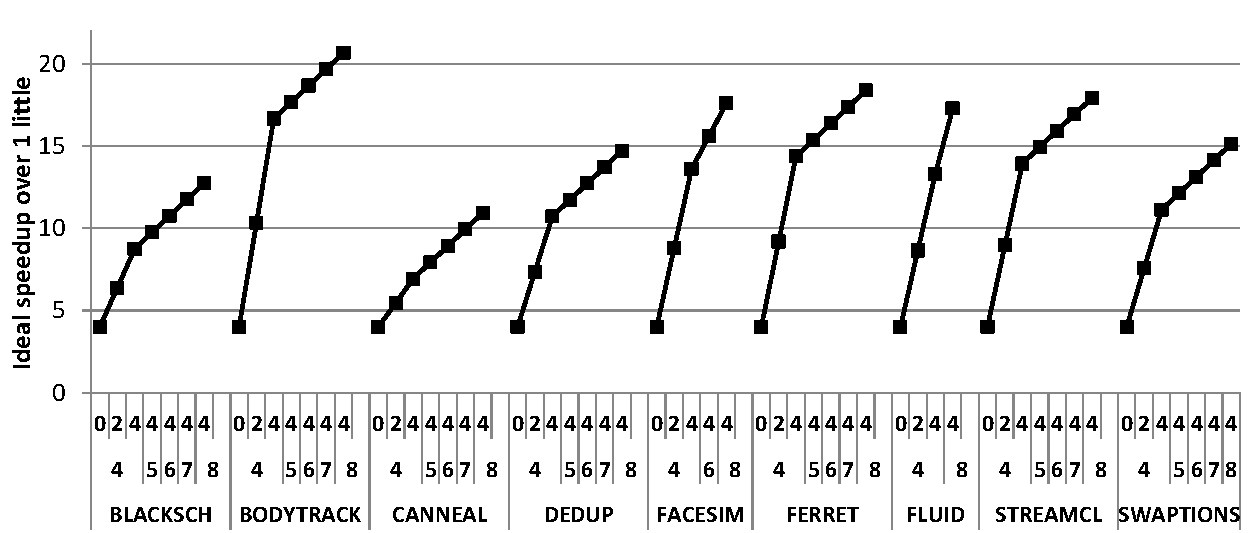
\includegraphics[width=1\columnwidth]{figures/ideal_speedup.pdf}
	\vspace{-0.5cm}
	\caption{Ideal speedup over 1 little core according to Equation~\ref{eq.ideal}. Numbers at the bottom of x axis show the total number of cores, numbers above it show the number of big cores}
	%Results are reported for systems with 0, 2 and 4 big cores, and a total number of cores between 4 and 8.}	
	\label{fig:ideal}%
	\vspace{-0.7cm}
\end{figure}

The original codes make use of the \texttt{pthreads} parallelization model for all the selected benchmarks. The taskified applications follow the same parallelization strategy implemented with OpenMP~4.0 task annotations.
The task-based implementation is done following two basic ideas: i) remove barriers where possible, by adding explicit data-dependencies; and ii) remove application-specific load balancing mechanisms, such as application-specific pools of threads implemented in \texttt{pthreads} and delegate this responsibility to the runtime.
%As a result, both codes achieve the same performance on homogeneous processors with a reduced number of cores~\cite{Chasapis:TACO2016}, while significantly reducing the total number of lines of code for benchmarks with application-specific load balancing mechanisms (bodytrack, dedup and ferret).

%%%%%%%%%%%%%%%%%%%%%%%%%%%%%%%%%%%%%%%%%%
%%%%%%%%%%%%%%%%%%%%%%%%%%%%%%%%%%%%%%%%%%
%\subsection{Performance Ratio Characterization}

When running on the big.LITTLE processor, each benchmark exhibits different performance ratios between big and little cores. These ratios tell us how many times faster a big core is compared to a little core. We measure the performance ratio of each application by executing it first on one big core and then on one little core, which corresponds to Speedup(0, 1, task-based) in Equation~\ref{eq.speedup}. 
% The equation for the performance ratio is the following:
% \begingroup\makeatletter\def\f@size{8}\check@mathfonts
% \begin{equation}
%   \text{Perf\_ratio(workload)} = \frac{\text{Exec. time(workload, 1little)}}{\text{Exec. time(workload, 1big)}}
%   \label{eq.perf_ratio}
% \end{equation}
% \endgroup
Table~\ref{tab:parsec} also includes the observed performance ratio for each application. Bodytrack is the application that benefits the most from running on the big core with a performance ratio of 4.16$\times$. The out-of-order execution of the big core together with an increased number of in-flight instructions significantly improves the performance of this application. In contrast, canneal is the benchmark with the lowest performance ratio, 1.73$\times$, as this is a memory-intensive benchmark that does not benefit as much from the extra computation power of the big core. In general, performance ratios are above 2.5$\times$ for seven out of nine benchmarks, reaching 3.03$\times$ on average. 

% In terms of power, the average ratio is significantly higher, 5$\times$, while the observed values vary between X and Y. \mm{Explain a bit more}.

Taking into account these performance ratios, we can estimate the ideal speedup of the platform for 
each workload assuming a perfect parallelization strategy. Equation \ref{eq.ideal} shows the 
equation for the ideal speedup over 1 little core computation according to the number of big (B) and 
little (L) cores.
\begingroup\makeatletter\def\f@size{8}\check@mathfonts
\begin{equation}
  \text{Ideal speedup(workload, B, L)} = \text{B $\times$ Perf\_ratio(workload) $+$ L}
\label{eq.ideal}
\end{equation}
\endgroup


Figure~\ref{fig:ideal} shows the ideal speedup of the system for each application for the varying 
numbers of cores. This speedup assumes that the applications are fully parallel with no barriers or 
other synchronization points. Thus, these speedups are an upper bound of the achievable application performance.
%As expected, benchmarks with higher performance ratios exhibit potentially higher speed-ups on the asymmetric multi-core.


%%%%%%%%%%%%%%%%%%%
%%%%%%%%%%%%%%%%%%%
\section{Evaluation}
\label{sec:evaluation}
\begin{figure*}[t]%
	\centering
	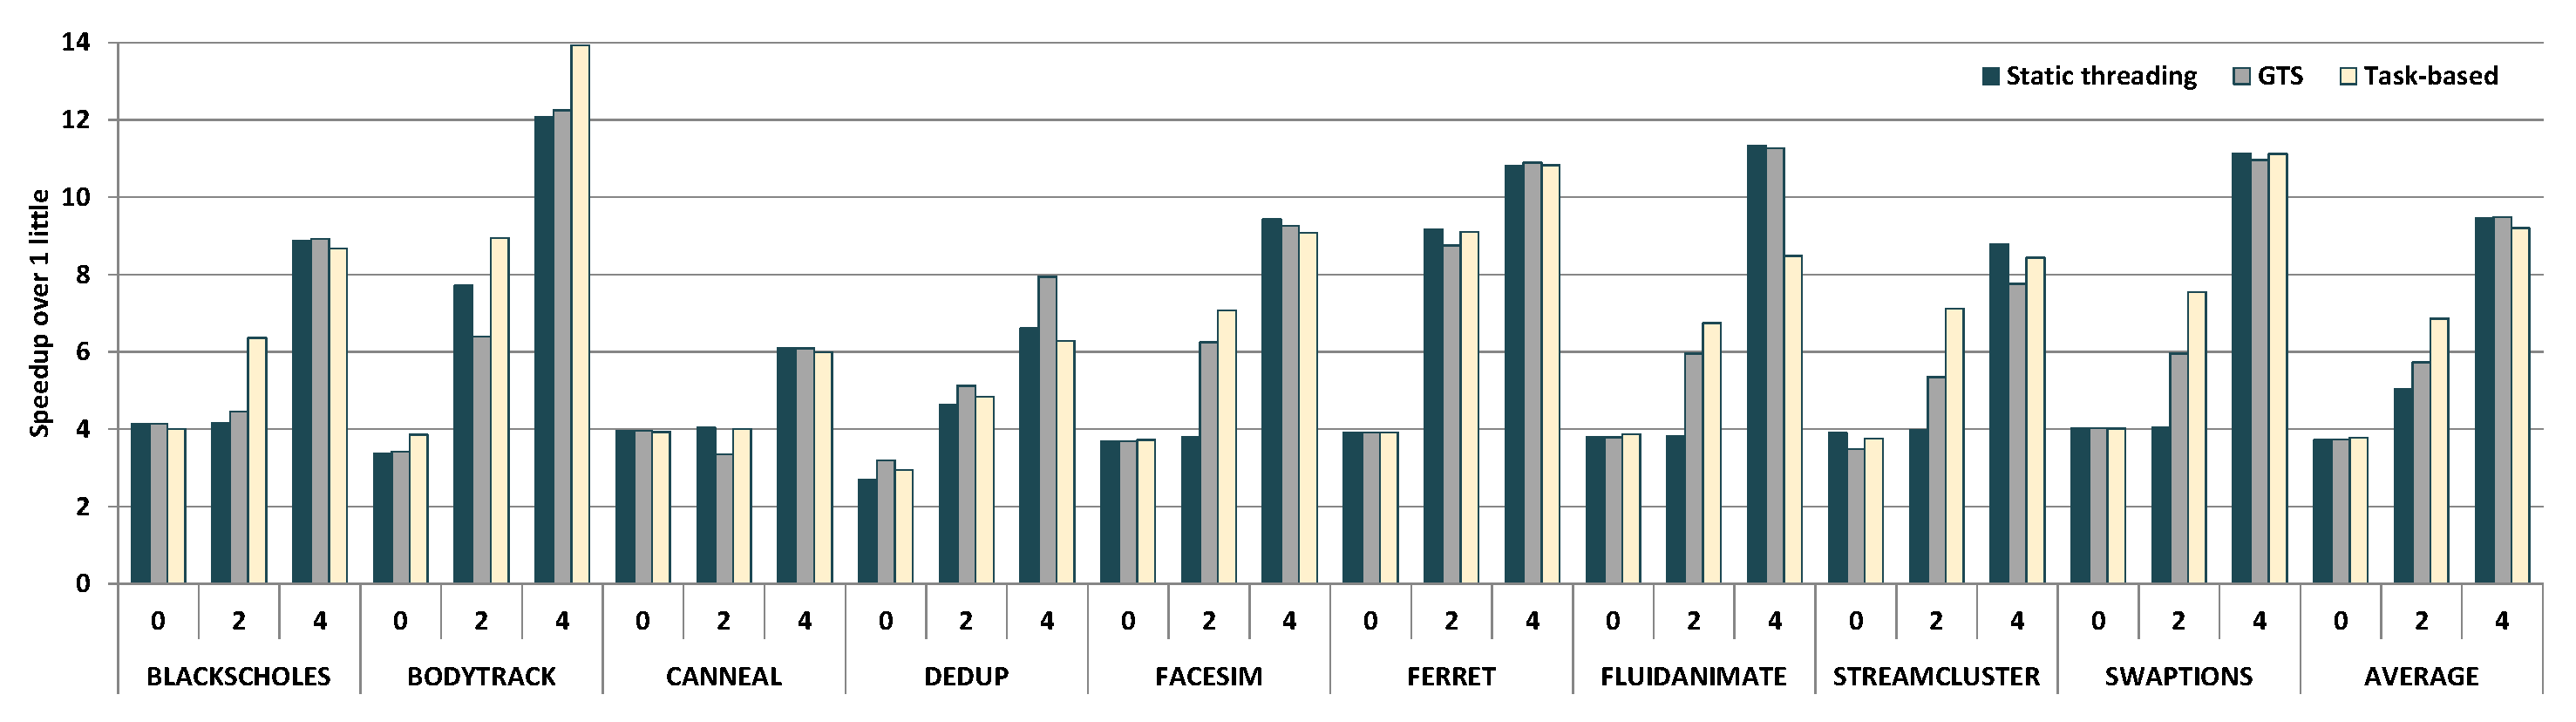
\includegraphics[width=1.0\textwidth]{figures/speedup-4.pdf}
	\vspace{-0.5cm}
	\caption{Execution time speedup over 1 little core for systems that consist of 4 cores in 
total with 0, 2 and 4 big cores. Different schedulers at the application (\textit{static 
threading}), OS  (\textit{GTS}) and runtime (\textit{task-based}) levels are considered.}
	%\caption{Performance improvements on a big.LITTLE processor with different $(F,N)$ configurations, where $F$ is the total number of big cores and $N$ the total number of cores. Results are normalized to running on four little cores with pinned Pthreads.}%
	\label{fig:speedup4}%
	\vspace{-0.3cm}
\end{figure*}



\begin{figure*}[t]%
	\centering
	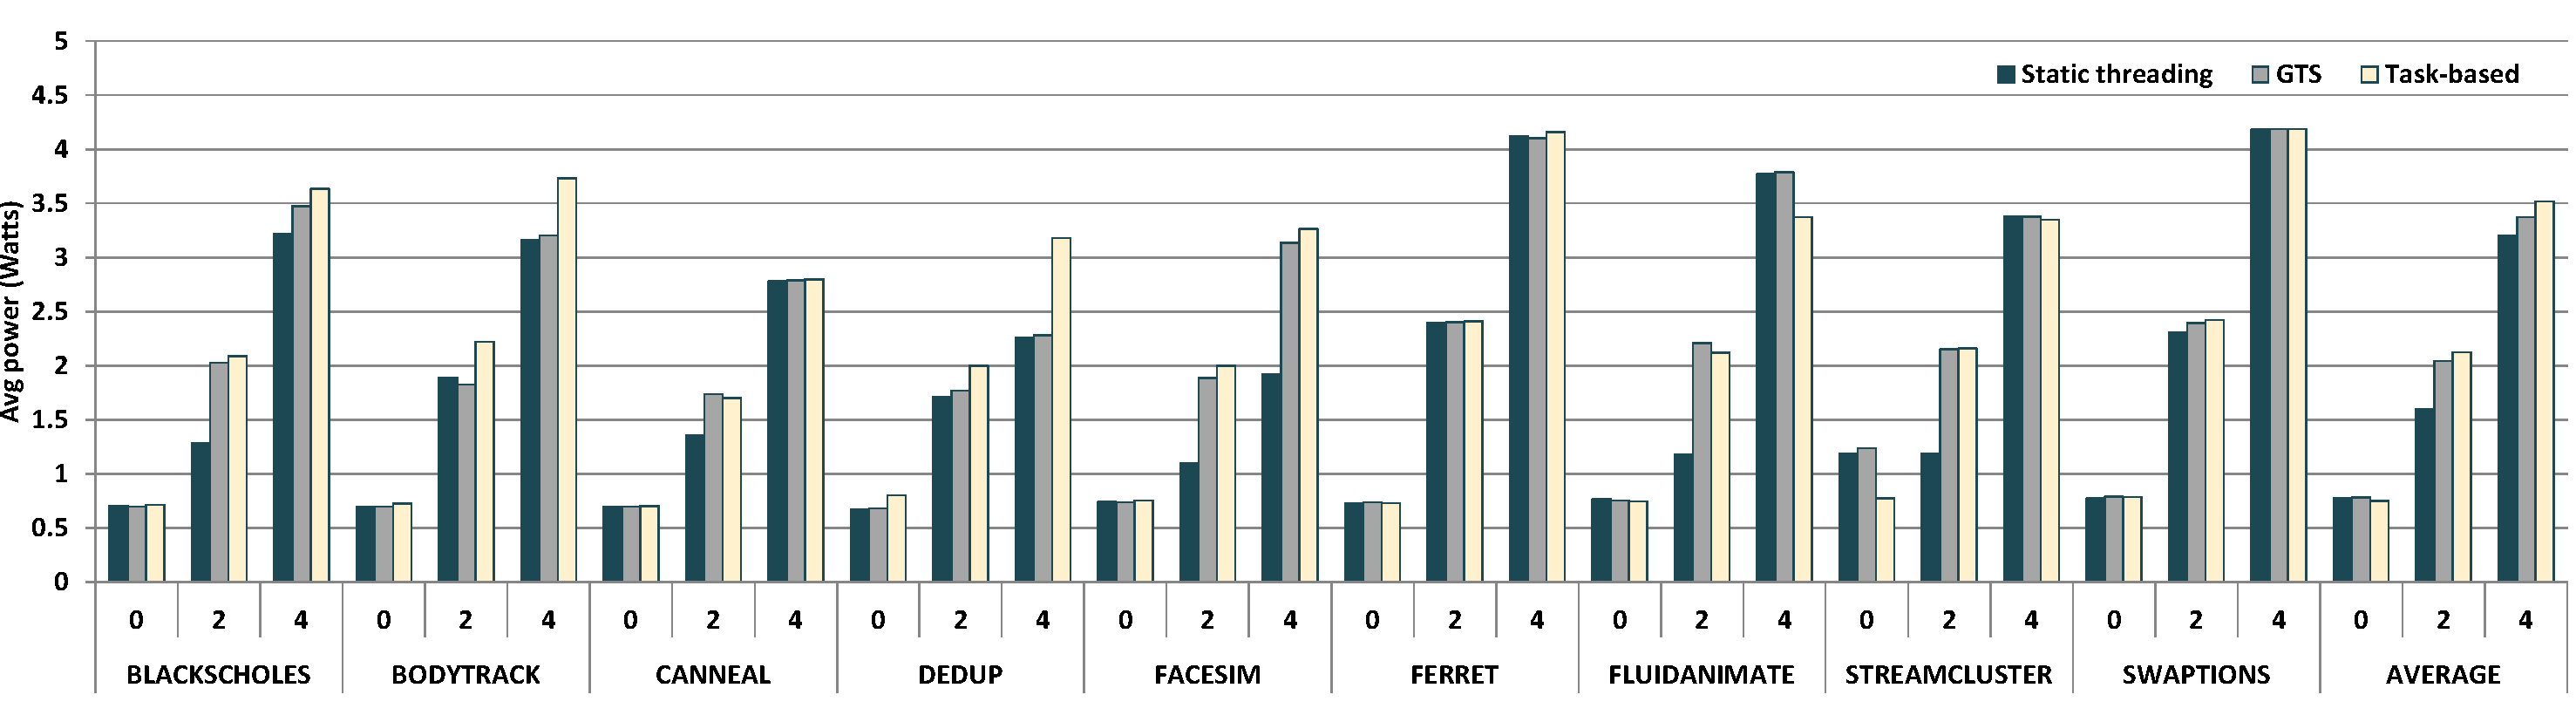
\includegraphics[width=1.0\textwidth]{figures/power4.pdf}
	\vspace{-0.5cm}
	\caption{Average power measurements on a 4-core system with 0, 2, and 4 big cores.}
	%\caption{Performance improvements on a big.LITTLE processor with different $(F,N)$ configurations, where $F$ is the total number of big cores and $N$ the total number of cores. Results are normalized to running on four little cores with pinned Pthreads.}%
	\label{fig:power4}%
	\vspace{-0.3cm}
\end{figure*}

\begin{figure*}[t]%
	\centering
	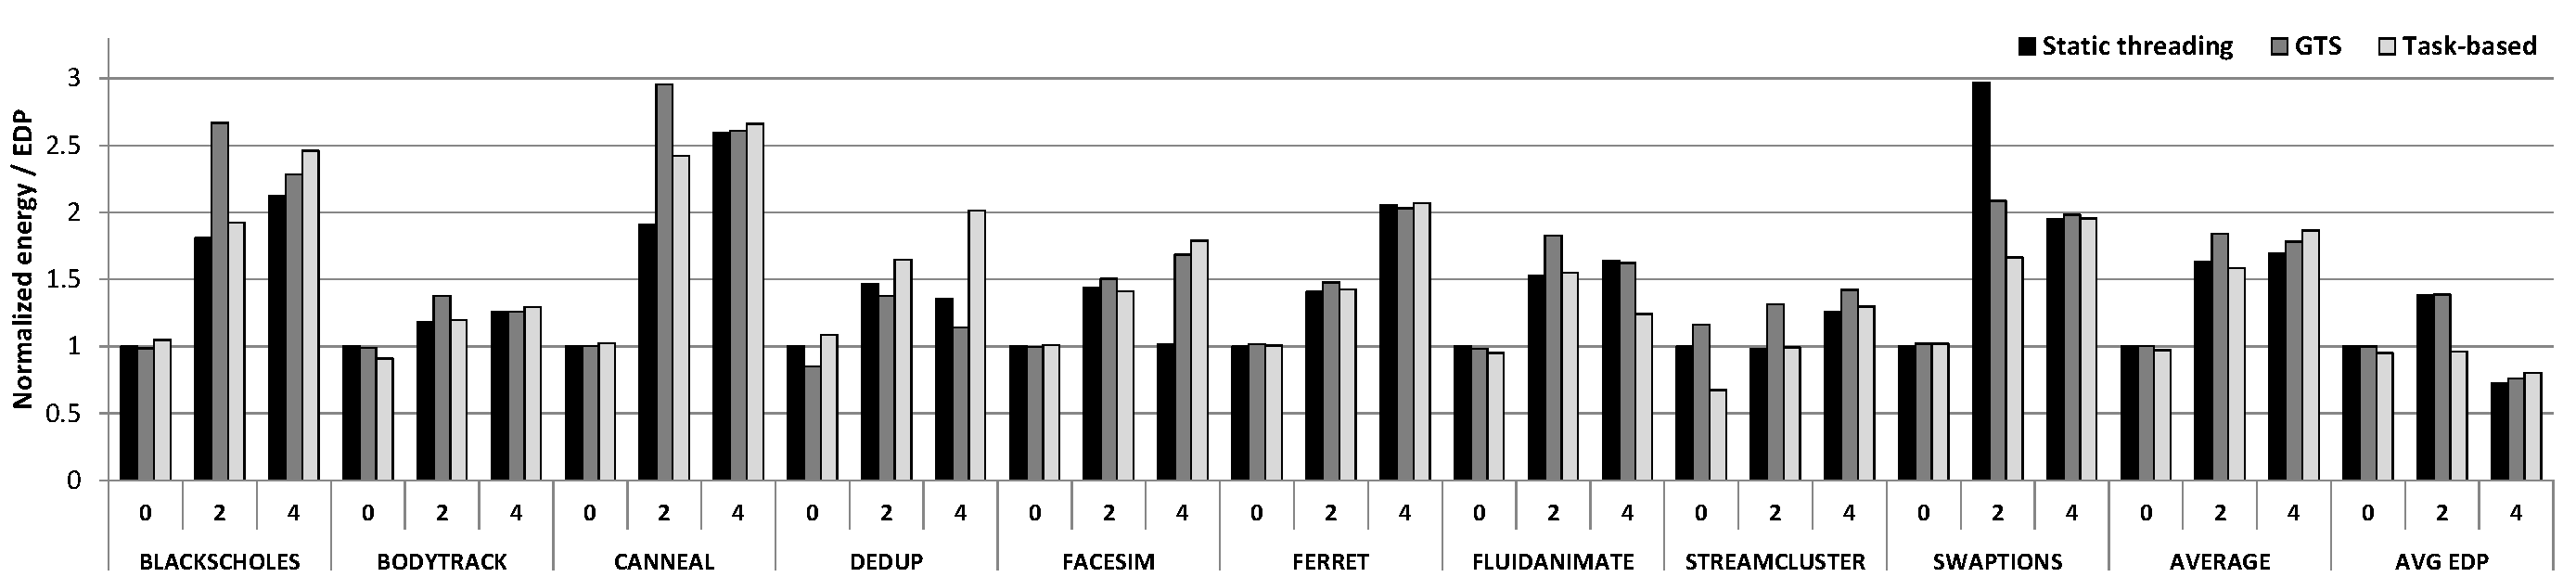
\includegraphics[width=1.0\textwidth]{figures/energy_EDP-4.pdf}
	\vspace{-0.5cm}
	\caption{Normalized energy consumption and average EDP on a 4-core system with 0, 2, and 4 big cores. Static threading on 4 little cores is the baseline in both cases. }
	%\caption{Performance improvements on a big.LITTLE processor with different $(F,N)$ configurations, where $F$ is the total number of big cores and $N$ the total number of cores. Results are normalized to running on four little cores with pinned Pthreads.}%
	\label{fig:energy4}%
	\vspace{-0.3cm}
\end{figure*}


% \mm{We don't need to include Figure~\ref{fig:edp4} as its average results are already in the previous figure.}
% \begin{figure*}[t]%
% 	\centering
% 	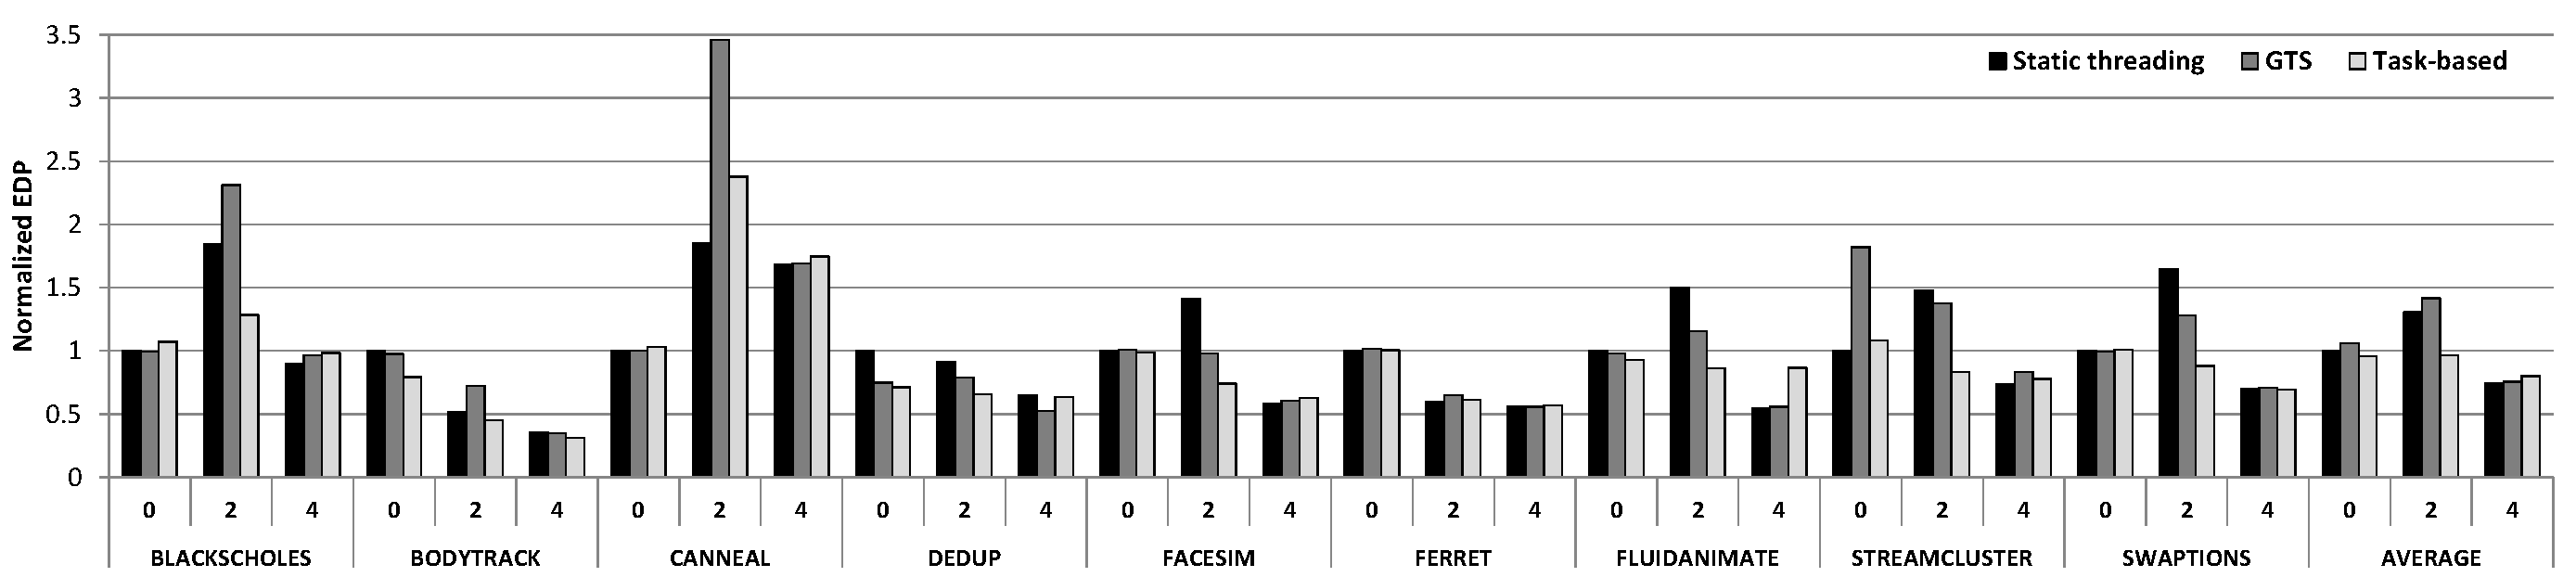
\includegraphics[width=1.0\textwidth]{figures/edp4.pdf}
% 	\vspace{-0.3cm}
% 	\caption{Normalized EDP on a 4-core system with 0, 2, and 4 big cores. Results are normalized with respect to static-threading EDP results with 4 little cores.}
% 	%\caption{Performance improvements on a big.LITTLE processor with different $(F,N)$ configurations, where $F$ is the total number of big cores and $N$ the total number of cores. Results are normalized to running on four little cores with pinned Pthreads.}%
% 	\label{fig:edp4}%
% \end{figure*}


% \begin{figure*}[t]%
% 	\centering
% 	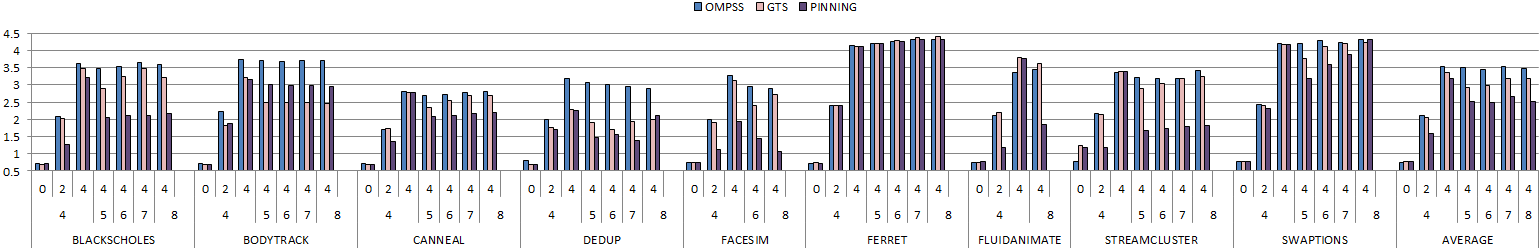
\includegraphics[width=1.0\textwidth]{figures/power-parsec}
% 	\vspace{-0.3cm}
% 	\caption{Average power consumption on a big.LITTLE processor with different $(F,N)$ configurations, where $F$ is the total number of big cores and $N$ the total number of cores.}%
% 	\label{fig:all-power}%
% \end{figure*}
% 
% \begin{figure*}[t]%
% 	\centering
% 	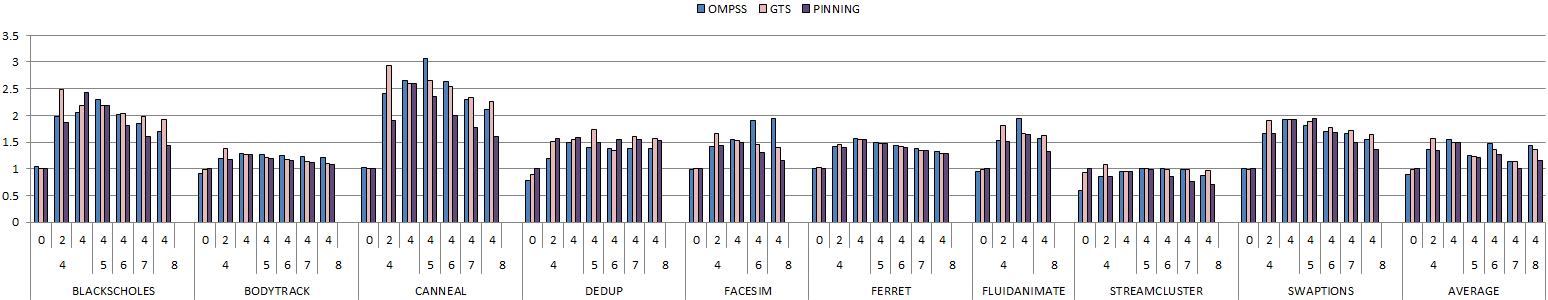
\includegraphics[width=1.0\textwidth]{figures/energy-parsec}%
% 	\vspace{-0.3cm}
% 	\caption{Energy consumption on a big.LITTLE processor with different $(F,N)$ configurations, where $F$ is the total number of big cores and $N$ the total number of cores. Results are normalized to running on four little cores with pinned Pthreads.}%
% 	\label{fig:all-energy}%
% \end{figure*}
% 
% 
% 
% \begin{figure*}[t]%
% 	\centering
% 	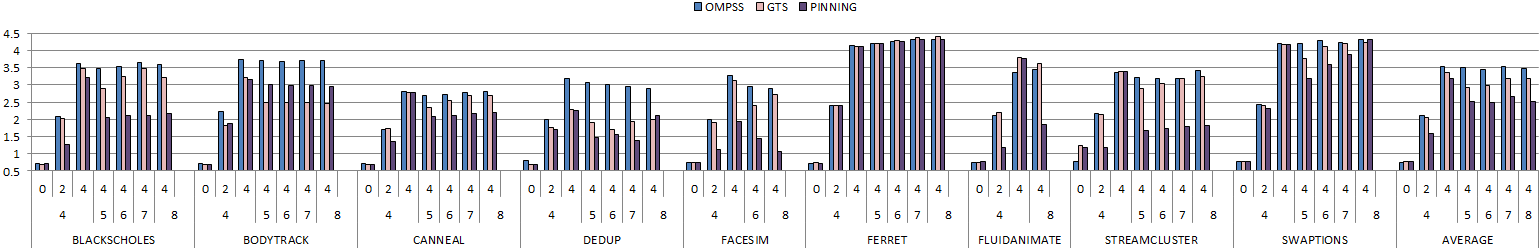
\includegraphics[width=1.0\textwidth]{figures/power-parsec}
% 	\vspace{-0.3cm}
% 	\caption{Average power consumption on a big.LITTLE processor with different $(F,N)$ configurations, where $F$ is the total number of big cores and $N$ the total number of cores.}%
% 	\label{fig:all-power}%
% \end{figure*}
% 
% \begin{figure*}[t]%
% 	\centering
% 	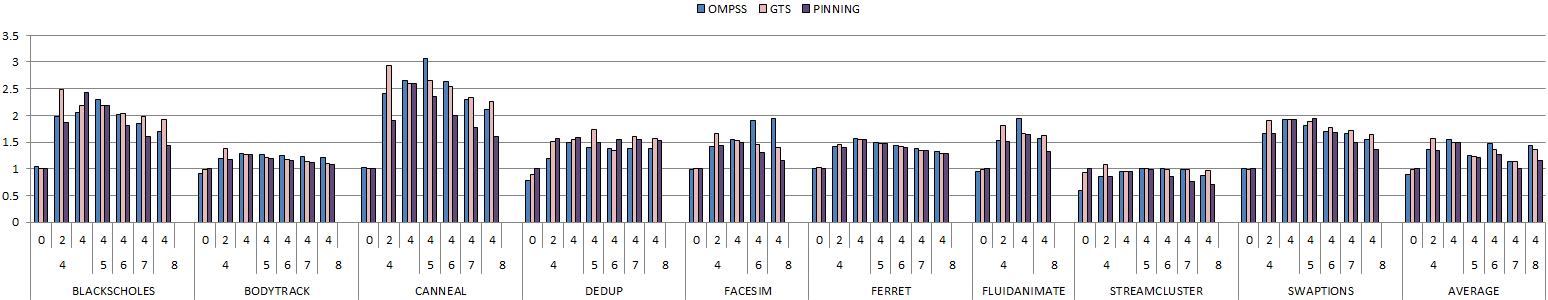
\includegraphics[width=1.0\textwidth]{figures/energy-parsec}%
% 	\vspace{-0.3cm}
% 	\caption{Energy consumption on a big.LITTLE processor with different $(F,N)$ configurations, where $F$ is the total number of big cores and $N$ the total number of cores. Results are normalized to running on four little cores with pinned Pthreads.}%
% 	\label{fig:all-energy}%
% \end{figure*}



We measure execution time, power, energy and EDP of nine 
applications from the PARSEC benchmark suite~\cite{Bienia:PhD2011}. We compare these metrics for 
three different scheduling approaches:
\begin{itemize}
\item \textit{Static threading}: scheduling decisions are made at the application level. The OS is not allowed to migrate threads between the clusters of big and little cores. 
\item \textit{GTS}\footnote{We choose to evaluate GTS instead of CS and IKS because it is the most advanced scheduling approach supported in the Linux kernel.}: dynamic coarse-grained OS scheduling 
using the GTS scheduler integrated in the Linux kernel~\cite{samsung, ARM} using the default 
PARSEC benchmarks. 
\item \textit{Task-based}: dynamic fine-grained scheduling at the runtime level with the task-based implementations of the benchmarks provided in PARSECSs~\cite{Chasapis:TACO2016}.
\end{itemize}


%%%%%%%%%%%%%%%%%%%%%%%%%%%%%%%%%%%%%%%%%%
%%%%%%%%%%%%%%%%%%%%%%%%%%%%%%%%%%%%%%%%%%
\subsection{Exploiting Parallelism in AMCs}
\label{sec:eval:A}
% \mm{This section should focus on identifying the problems that current applications have on an asymmetric/heterogeneous multicore. For example, static scheduling, homogeneous domain/workload partition. More dynamic applications, will scale better (bodytrack, dedup, ferret, freqmine, vips).}

This section examines the opportunities and challenges that current AMCs offer to emerging parallel applications. With this objective, we first evaluate a system with a constant number of four cores, changing the level of asymmetry to evaluate the characteristics of each configuration. In these experiments, all applications run with the original parallelization strategy that relies on the user to balance the application (\emph{Static threading}). We also evaluate the OS-based dynamic scheduling (\emph{GTS}) and the task-based runtime dynamic scheduling (\emph{Task-based}) for the same applications. 
% Figure~\ref{fig:ideal} shows the ideal speedup of the system for all the different combination of big and little cores. 
The system configurations evaluated in this section are:
i)~Four little cores (\texttt{0+4}); ii)~Two big and two little cores (\texttt{2+2}); and iii)~Four 
big cores (\texttt{4+0})

% \begin{itemize}
% \item Four little cores (\texttt{0+4})
% \item Two big and two little cores (\texttt{2+2})
% \item Four big cores (\texttt{4+0})
% \end{itemize}
For these configurations, Figure~\ref{fig:speedup4} shows the speedup of the PARSEC benchmarks with respect to running on a single little core. Figure~\ref{fig:power4} reports the average power dissipated on the evaluated platform. Finally, Figure~\ref{fig:energy4} shows the total energy consumed per application for the same configurations. Energy results are normalized to the energy measured with four little cores (higher values imply higher energy consumptions). Average EDP results are also included in this figure.

Focusing on the average performance results, we notice that all approaches perform similarly for the homogeneous configurations. 
Specifically, applications obtain the best performance on the configuration~\emph{4+0}, with an average speedup of 9.5$\times$ over one little core. 
When using four little cores, an average speedup of 3.8$\times$ is reached for all approaches. 
This shows that all the approaches are effective for this core count. 
In the configuration~\emph{2+2}, \emph{Static threading} slightly improves performance (5.0$\times$ speedup), while \emph{GTS} and \emph{Task-based} reach significantly higher speedups: 5.9$\times$ and 6.8$\times$, respectively.

Contrarily, in terms of power and energy, the most efficient configuration is running with four little cores, as the performance ratio between the different cores is inversely proportional to the power ratio~\cite{Greenhalgh2011}. On average, all the approaches reach a power dissipation of 0.75W for the \texttt{0+4} configuration, while \emph{Task-based} reaches 3.5W for the \texttt{4+0} configuration which is the one with the highest average power dissipation. In configuration \texttt{2+2}, average energy values for \emph{Static threading} and \emph{Task-based} are nearly the same, as the increase in power from 1.6W to 2.1W is compensated by a significant improvement in performance of 30\%.

Finally, in terms of EDP using the four big cores is the optimal, as the performance improvements compensate the increase in total energy. 
In configuration \texttt{2+2}, \emph{Task-based} achieves the same EDP results as in \texttt{0+4}, but with 81\% better performance. 
For the asymmetric configuration, \emph{Task-based} achieves the best performance-energy combination since its dynamic scheduling is effectively utilizing the little cores. 

%\texttt{0+4} reaches a power dissipation of 0.75W with all approaches, while \emph{Task-based} reaches 3.5W in configuration \texttt{4+0}.

%\kc{Consider removing this paragraph? It just mentions the obvious results that reviewers are complaining about...} Thus, if the number of cores remains constant, the best configuration in terms of performance and EDP corresponds to a symmetric configuration with big cores (e.g. \texttt{4+0}), while in terms of power and energy the best configuration corresponds to a symmetric configuration with little cores (e.g. \texttt{0+4}). 
% From the average energy-delay product (EDP) results in Figure~\ref{fig:energy4} we can approximate the configuration that achieves the highest performance with the best possible energy consumption. The configuration with the lowest EDP is the one with four big cores (\texttt{4+0}) since all the scheduling approaches manage to compensate the additional energy consumption with the speedup that can be achieved on this set-up. However, it is interesting to note that for the asymmetric configuration the \emph{Task-based} approach achieves the best combination of performance and energy since its dynamic scheduling approach is effectively utilizing the little cores. 

\begin{figure*}[t]%
	\centering
	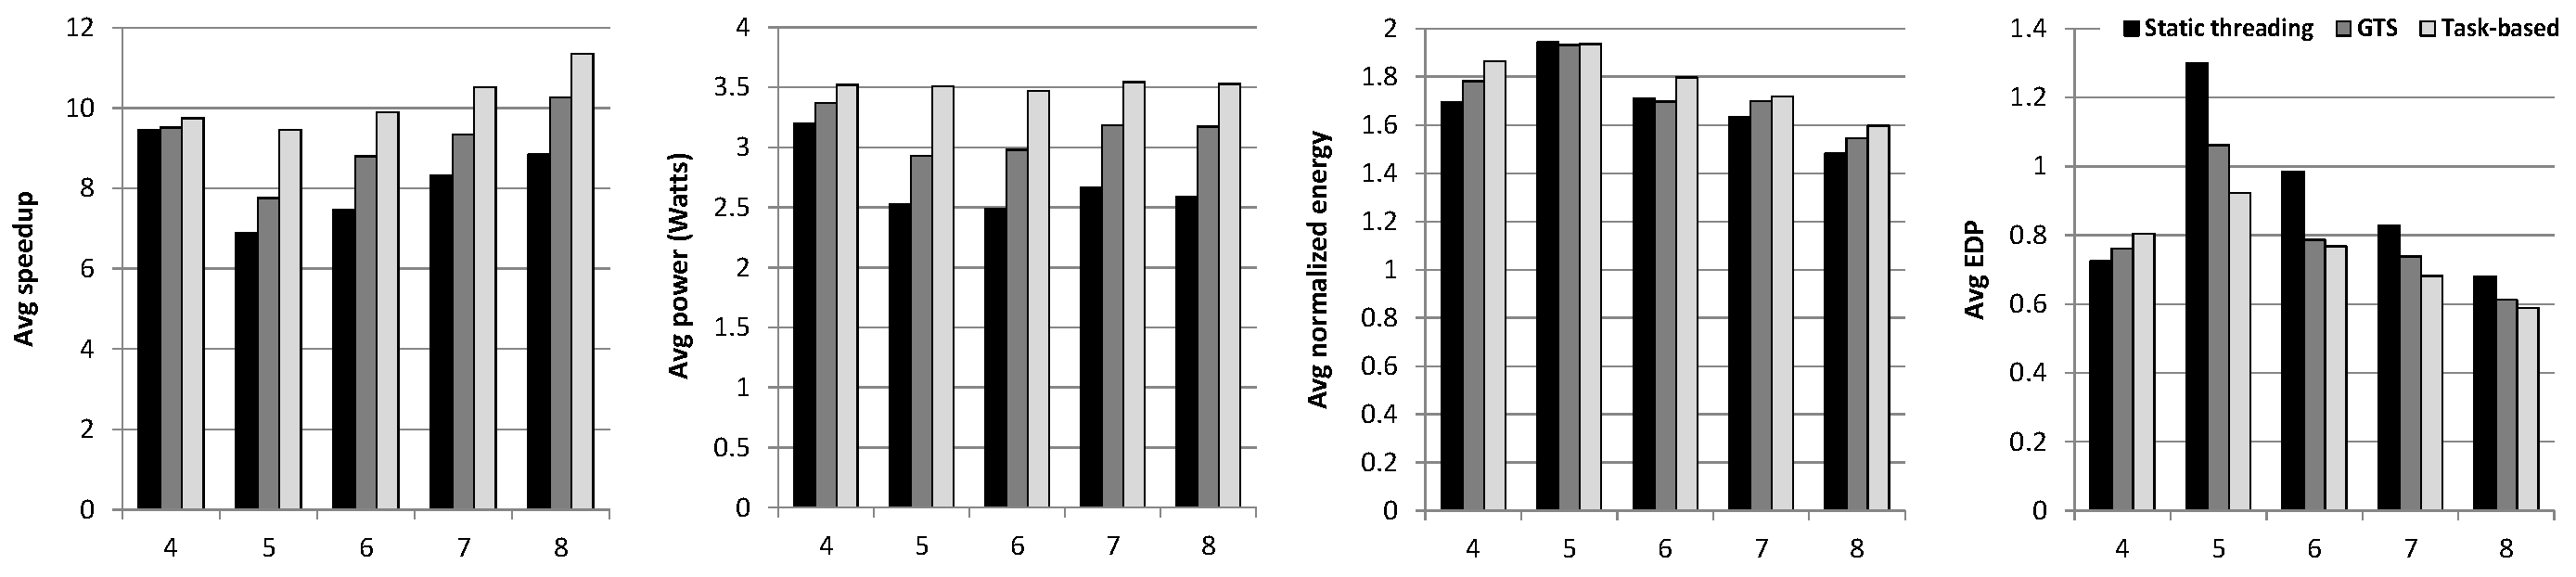
\includegraphics[width=\textwidth]{figures/averages_4plus.pdf}
	\vspace{-0.5cm}
	\caption{Average results when running on 4 to  8 cores with 4 of them big. Speedup is over 1 little core. Static threading on 4 little cores is the baseline of energy consumption and EDP}
	%\caption{Performance improvements on a big.LITTLE processor with different $(F,N)$ configurations, where $F$ is the total number of big cores and $N$ the total number of cores. Results are normalized to running on four little cores with pinned Pthreads.}%
	\label{fig:averages4plus}%
	\vspace{-0.3cm}
\end{figure*}


Next, we focus on the obtained results per benchmark. 
For applications with an extensive use of barriers (blackscholes, facesim, fluidanimate, streamcluster and swaptions) or with a memory intensive pattern (canneal), the extra computational power offered by the big cores in configuration \texttt{2+2} is not exploited. 
As a result with \emph{Static threading} performance is only slightly improved by 1\% on average when moving from \texttt{0+4} to the \texttt{2+2} configuration. 
This slight improvement comes at the cost of much more power and energy consumption (79\% and 77\% respectively).
%As a result, with \emph{Static threading} the performance equals the one of the configuration \texttt{0+4} (average 1\% improvement), but at the expense of much more power and energy consumption (79\% and 64\% increase, respectively). 
These results are explained three-fold: i) load is distributed homogeneously among threads in some 
applications; ii) extensive usage of barriers force big cores to wait until little cores reach the 
barrier; and iii) high miss rates in the last-level cache cause frequent pipeline stalls and prevent 
to fully exploit the computational power of big cores. 
To alleviate these problems, the programmer should develop more advanced parallelization strategies that could benefit from AMCs, as performed in the remaining applications, or rely on dynamic scheduling at OS or runtime levels.

The three remaining applications are parallelized using a pipeline model (bodytrack, dedup, and ferret)  with queues for the data-exchange between pipeline stages and application-specific load balancing mechanisms designed by the programmer. As a result, \emph{Static scheduling} with these applications benefits from the extra computational power of the big cores in the configuration \texttt{2+2}. These mechanisms are not needed in the \emph{Task-based} code; in this approach the code of the application is simplified and the runtime automatically allows the overlapping of the different pipeline stages. Thus, on the asymmetric configuration, \emph{Task-based} further improves the obtained performance, reaching a 13\% average improvement over \emph{GTS}. Clearly, these applications benefit in performance by the increased number of big cores, while power and energy are increasing since the big cores are effectively utilized.

%In these applications, all the approaches clearly outperform configuration \texttt{0+4}, while still increasing power and energy, as now all cores are busy (not only the little ones).

%the parallel regions to overlap more aggressively different stages of the pipeline. As a result, \emph{Task-based} further improves the obtained performance, reaching a 13\% average speedup over \emph{GTS}. In these applications, all the approaches clearly outperform configuration \texttt{0+4}, while still increasing power and energy, as now all cores are busy (not only the little ones).

Generally, relying on the programmer to statically schedule asymmetric configurations does not report good results, as it 
is very hard to predict the system's behaviour at application-level. 
Only applications that implement advanced features with user-level schedulers and load balancing techniques, can benefit from asymmetry, at the cost of programmability effort. 
Relying on the OS scheduler is a suitable alternative without code modifications, but relying on the runtime to dynamically schedule tasks on the asymmetric processor achieves much better performance, power and energy results.

%the developer did not consider it when designing the parallelization technique. When applications implement advanced features with user-level schedulers and load balancing techniques, applications can benefit from asymmetry, of course at the cost of programmability effort. A suitable alternative consists in relying on the OS system or the runtime to dynamically schedule tasks into the asymmetric processor, reaching much better performance, power and energy results in these systems.


%To estimate the best configuration when taking into account both performance and energy efficiency we have to 


%Relying on the programmer to benefit from asymmetry does not report good results, as the developer did not consider it when designing the parallelization technique. When applications implement advanced features with user-level schedulers and load balancing techniques, applications can benefit from asymmetry, of course at the cost of programmability effort. A suitable alternative consists in relying on the OS system or the runtime to dynamically schedule tasks into the asymmetric processor, reaching much better performance, power and energy results in these systems.

%, power or energy corresponds to a homogeneous configuration with in-order cores (power and energy) or big cores (performance). 

%In general relying on the programmer to benefit from asymmetry does not report good results, as the developer did not consider it when designing the parallelization technique. When applications implement advanced features with user-level schedulers and load balancing techniques, applications can benefit from asymmetry, of course at the cost of programmability effort. A suitable alternative consists in relying on the OS system or the runtime to dynamically schedule tasks into the asymmetric processor, reaching much better performance, power and energy results in these systems.
\iffalse
\mm{Figure~\ref{fig:energy4} also shows the average normalized results for EDP. In this case, lower is better. I didn't comment these results yet. With this metric, Task-based on 2+2 is as good as the others in 0+4 while we obtain better performance. This is interesting, but I'm not sure if it adds much with respect to the already presented numbers.}

\mm{I haven't commented much the results with the GTS scheduler. Maybe we should extend this part. Next, I put some sentences that might be useful, although I don't know where to put them.}

As described in Section~\ref{sec:scheduling}, the Global Task Scheduler (GTS) migrates tasks between cores in order to balance the load in the different cores of the heterogeneous processor. 

For fork-join + homogeneous load, the scheduler should be very effective, reaching the performance results of OmpSs. However, it is unaware of what it is moving around, which means that it might move a thread that is idle to a big core...

Consequently, for some benchmarks, the OS is making decisions without coordinating with the application scheduler and can worsen the performance. This should be the case of the applications with advanced load balancing techniques, but I still don't know if we will see this behavior.
\fi
\begin{figure*}[t]%
	\centering
	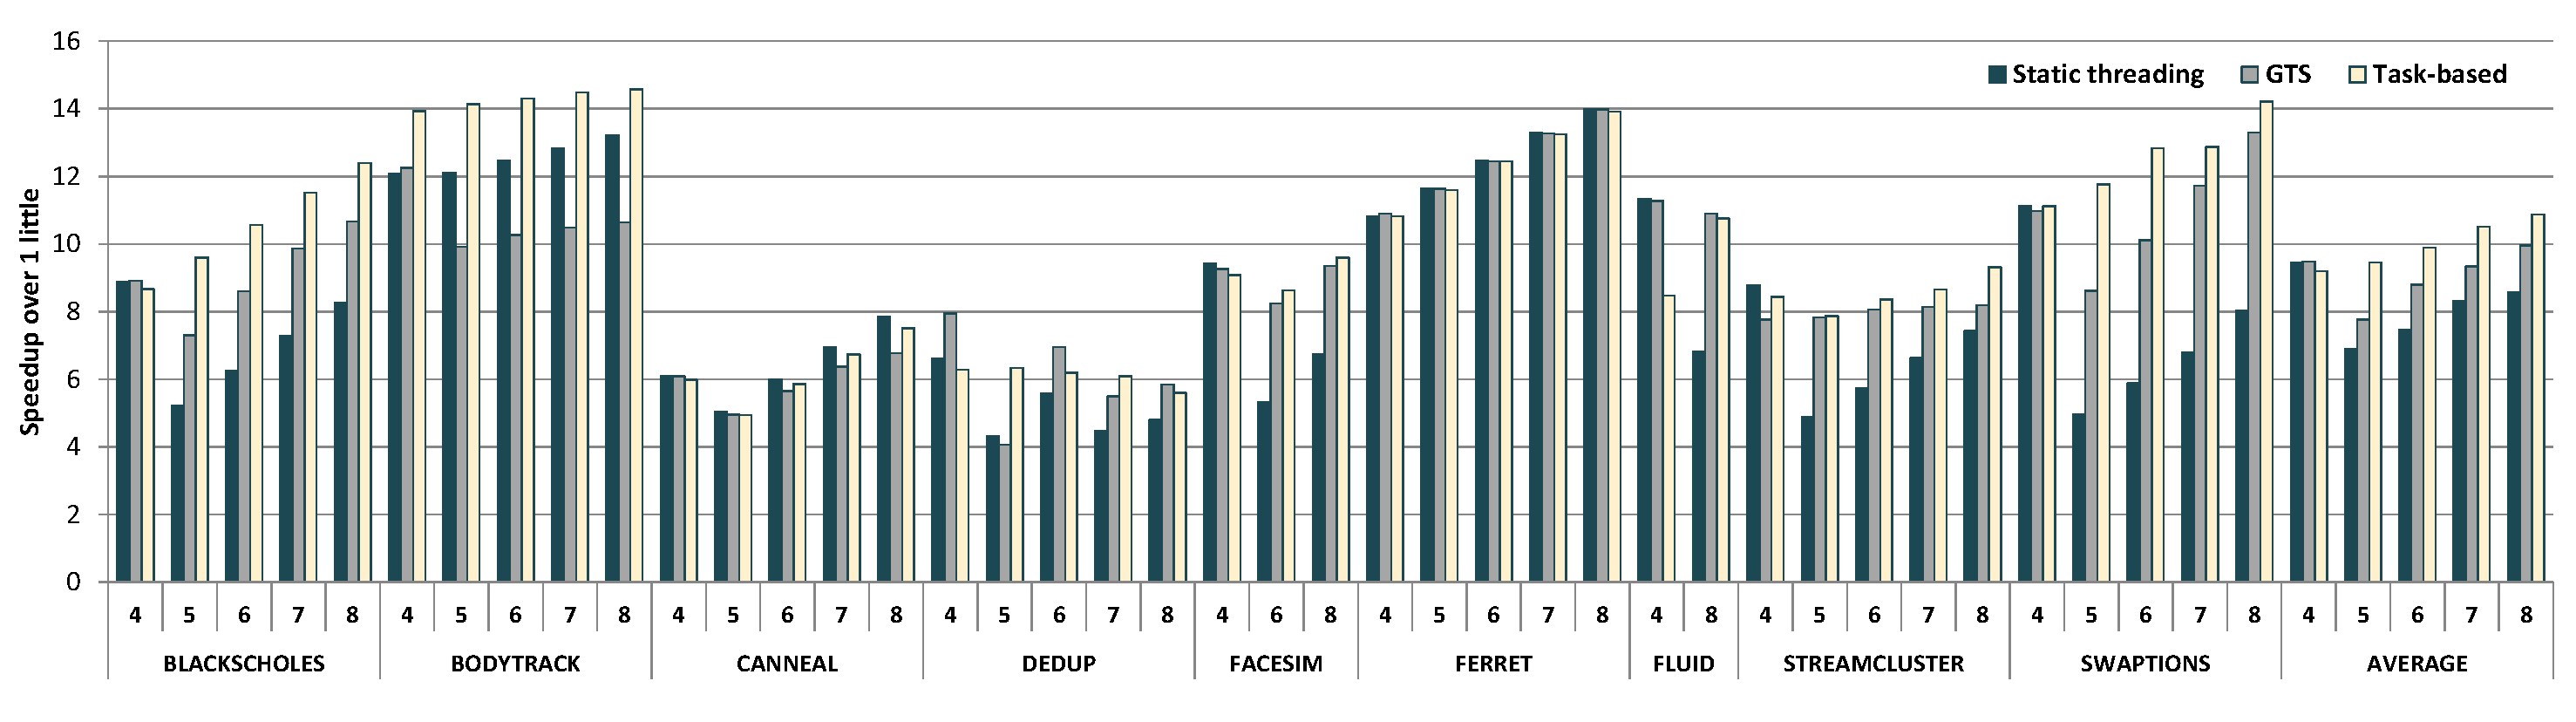
\includegraphics[width=1.0\textwidth]{figures/speedup-4plus.pdf}
	\vspace{-0.5cm}
	\caption{Speedup over 1 little core when running on 4 to 8 cores and 4 of them are big}
	%\caption{Performance improvements on a big.LITTLE processor with different $(F,N)$ configurations, where $F$ is the total number of big cores and $N$ the total number of cores. Results are normalized to running on four little cores with pinned Pthreads.}%
	\label{fig:speedup4plus}%
	\vspace{-0.3cm}
\end{figure*}

\begin{figure*}[t]%
	\centering
	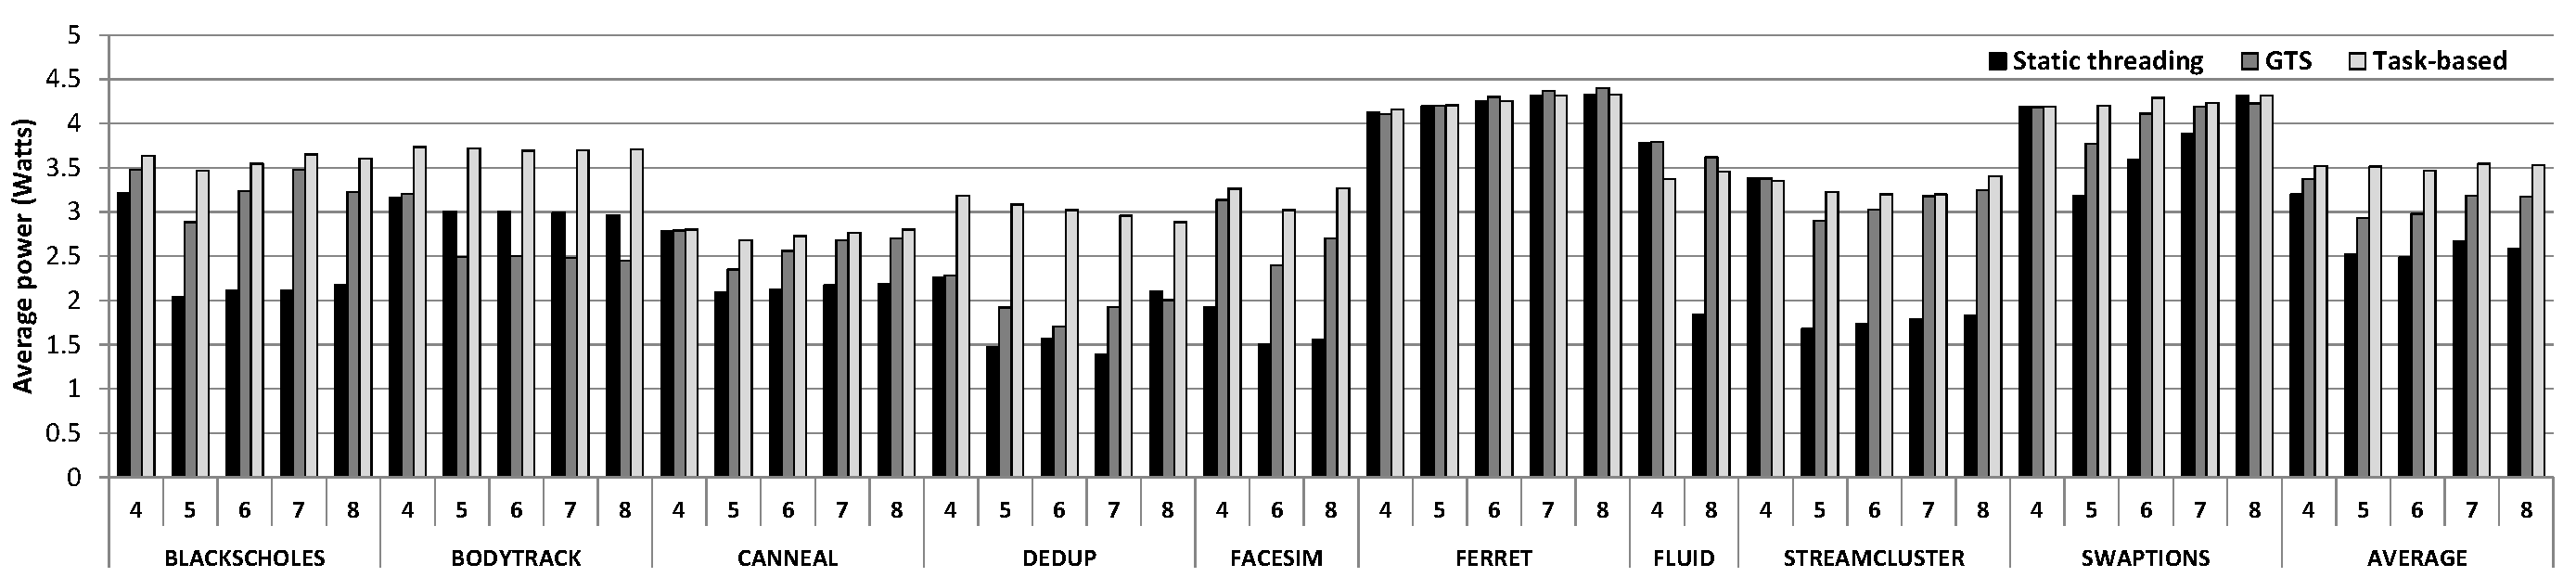
\includegraphics[width=1.0\textwidth]{figures/power4plus.pdf}
	\vspace{-0.5cm}
	\caption{Average power when running on 4 to 8 cores and 4 of them are big}
	%\caption{Performance improvements on a big.LITTLE processor with different $(F,N)$ configurations, where $F$ is the total number of big cores and $N$ the total number of cores. Results are normalized to running on four little cores with pinned Pthreads.}%
	\label{fig:power4plus}%
	\vspace{-0.5cm}
\end{figure*}

% \begin{figure*}[t]%
% 	\centering
% 	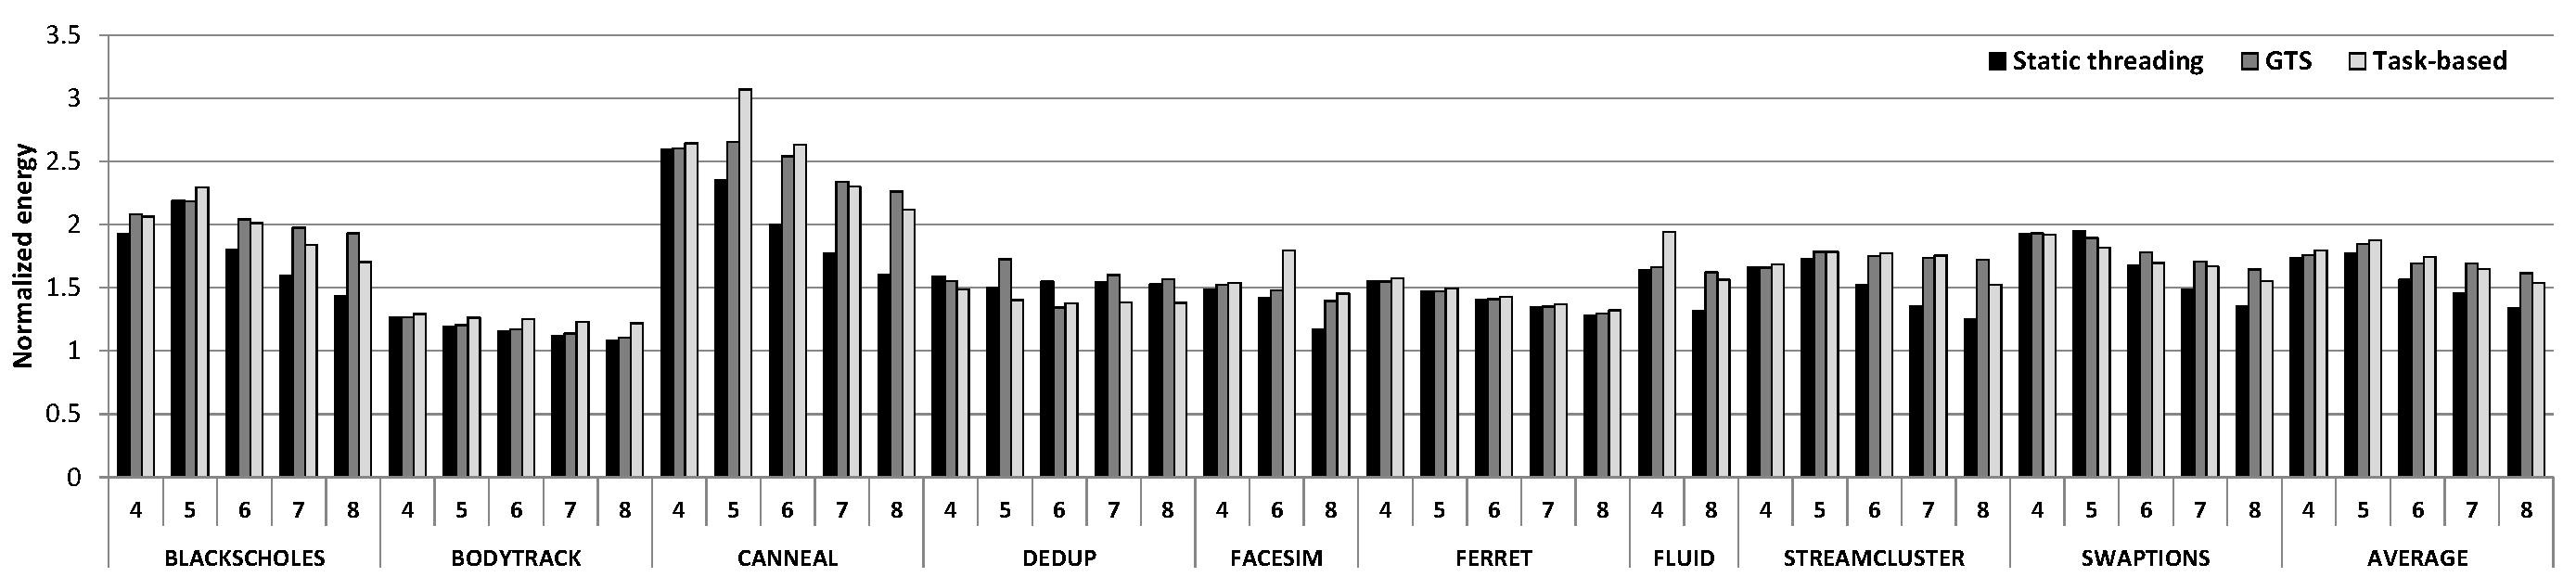
\includegraphics[width=1.0\textwidth]{figures/energy-4plus.pdf}
% 	\vspace{-0.5cm}
% 	\caption{Normalized energy consumption with respect to 4-little-static-threading energy consumption, when running on 4 to 8 cores and 4 of them are big}
% 	%\caption{Performance improvements on a big.LITTLE processor with different $(F,N)$ configurations, where $F$ is the total number of big cores and $N$ the total number of cores. Results are normalized to running on four little cores with pinned Pthreads.}%
% 	\label{fig:energy4plus}%
% 	\vspace{-0.3cm}
% \end{figure*}

% \begin{figure*}[t]%
% 	\centering
% 	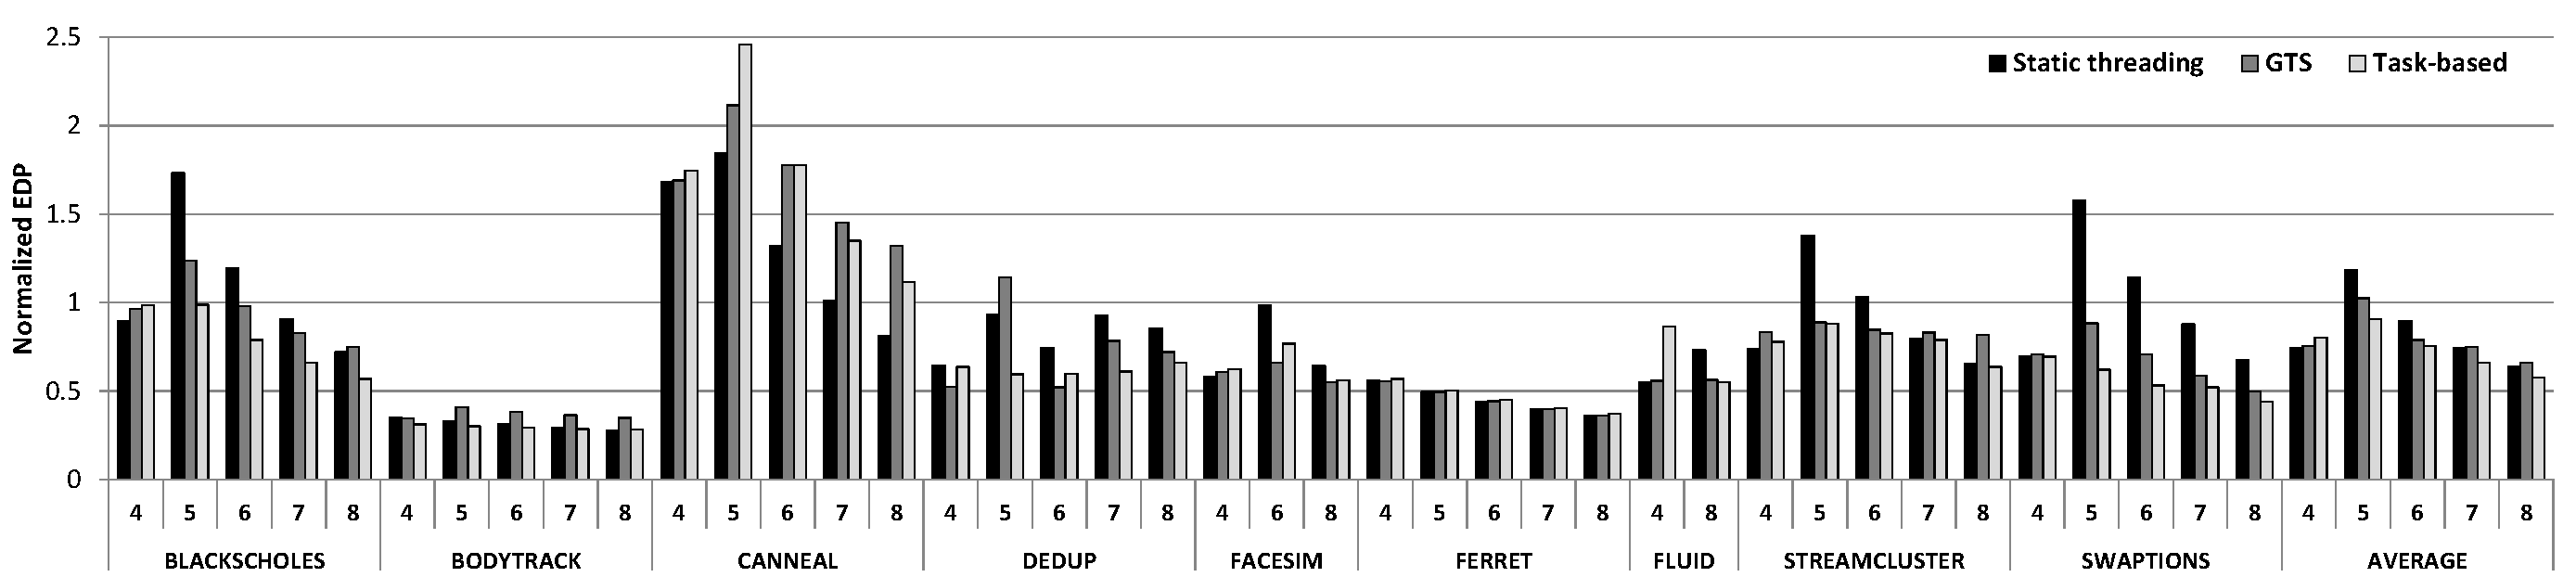
\includegraphics[width=1.0\textwidth]{figures/edp4plus.pdf}
% 	\vspace{-0.3cm}
% 	\caption{Normalized EDP when running on 5, 6, 7, or 8 cores and 4 of them are big}
% 	%\caption{Performance improvements on a big.LITTLE processor with different $(F,N)$ configurations, where $F$ is the total number of big cores and $N$ the total number of cores. Results are normalized to running on four little cores with pinned Pthreads.}%
% 	\label{fig:edp4plus}%
% \end{figure*}


%%%%%%%%%%%%%%%%%%%%%%%%%%%%%%%%%%%%%%%%%%
%%%%%%%%%%%%%%%%%%%%%%%%%%%%%%%%%%%%%%%%%%
\subsection{Adding Little Cores to an SMC}

In the following experiments, we explore if an application running on a symmetric multi-core (SMC) with big cores can benefit from adding small cores that help in its execution. Having more computational resources increases the ideal speedup a parallel application can reach, but it also introduces challenges at application, runtime and OS level. 
Thus, we examine how many small cores have to be added to the system to compensate the cons of having to deal with AMCs.

To evaluate this scenario, we explore configurations \texttt{4+0}, \texttt{4+1}, \texttt{4+2}, \texttt{4+3} and \texttt{4+4}. In these experiments, the number of big cores remains constant (four), while the number of little cores increases from 0 to 4. First we focus on the average results of speedup, power, energy and EDP, shown in Figure~\ref{fig:averages4plus}.

The speedup chart of Figure~\ref{fig:averages4plus} shows that \emph{Static threading} does not benefit from adding little cores to the system.
In fact, this approach brings an average 6\% slowdown when adding four little cores for execution (\texttt{4+4}).
This is a result of the static thread scheduling; because the same amount of work is assigned to each core, when the big cores finish the execution of their part, they become idle and under-utilized. 
GTS achieves a limited speedup of 8\% with the addition of four little cores to the \texttt{4+0} configuration. The addition of a single little core brings a 22\% slowdown (from \texttt{4+0} to \texttt{4+1}) and requires three additional little cores to reach the performance of the symmetric configuration (\texttt{4+3}).  Finally, the \emph{Task-based} approach always benefits from the extra computational power as the runtime automatically deals with load imbalance. Performance improvements keep growing with the additional little cores, reaching an average improvement of 15\% over the symmetric configuration when 4 extra cores are added. 
%An interesting observation is that according to the ideal speedup (Equation~\ref{eq.ideal} and Figure~\ref{fig:ideal}), the average ideal performance increase when moving from the \texttt{4+0} configuration to the \texttt{4+4} is 33\%, considering that the average performance ratio is 2.96$\times$ as shown in Table~\ref{tab:parsec}. Thus, the task-based approach achieves almost half of this theoretical ideal performance.

%the execution time speedup of the PARSEC benchmarks with respect to running in a single in-order core. 
%When looking at the average results, it is very interesting to see that the \emph{Static threading} approach clearly fails to benefit from the extra in-order cores. Even with four extra cores (configuration \texttt{4+4}), an average 15\% slowdown is obtained. \emph{GTS} also suffers a significant performance reduction when adding an extra little core (22\% slowdown) and requires three additional little cores to match the performance of the symmetric configuration. With an additional extra core, \emph{GTS} reaches an average 5\% speedup over the symmetric configuration. 



%In contrast, the \emph{Task-based} approach always benefits from the extra computational power as the runtime automatically deals with load imbalance. Performance improvements keep growing with the additional little cores, reaching an average improvement of 16\% over the symmetric configuration when 4 extra cores are added. Please, note that according to Table~\ref{tab:parsec} the performance ratio between big and little cores is 2.96$\times$, which means that the ideal speedup when adding 4 little cores to a system with 4 big cores is 1.33$\times$ ($\frac{2.96\cdot 4 + 4}{2.96\cdot 4}$). Thus, the \emph{Task-based} approach reaches half of the potential speedup on this asymmetric platform.

The power chart of Figure~\ref{fig:averages4plus} shows oppositional benefits among the three approaches. We can see that \emph{Static threading} and \emph{GTS} benefit from asymmetry, effectively reducing average power consumption.
\emph{Static threading} reduces power consumption when moving from the \texttt{4+0} to the \texttt{4+4} system by 23\% while \emph{GTS} does so by 6.2\%.
On the other hand, the \emph{task-based} approach keeps the big cores busy for most of the time so it maintains the average power nearly constant.



%In terms of power, the tradeoffs completely change. As shown in Figure~\ref{fig:power4plus}, \emph{Static threading} and \emph{GTS} always benefit from asymmetry, effectively reducing average power consumption. On average in configuration \texttt{4+4}, \emph{Static threading} and \emph{GTS} reduce power 23\% and 6.2\%, respectively, with respect to the symmetric multi-core. In contrast, the \emph{Task-based} approach always has all big cores busy and maintains overall power nearly constant. 

%In terms of energy, the third chart of Figure~\ref{fig:averages4plus} shows that the \emph{Static threading} significantly reduces energy consumption by 31\% when moving from \texttt{4+0} to the \texttt{4+4} configuration. As shown in the previous section, little cores are more energy efficient than big cores, at the cost of reduced performance. In the case of \emph{GTS} and \emph{Task-based}, at least two extra cores are needed to reduce energy. 
% In configuration \texttt{4+4}, energy is reduced by 31\% for \emph{Static threading}, 9.3\% for \emph{GTS}, and 16\% for \emph{Task-based}. Consequently, we can state that asymmetry reduces overall energy consumption, although the best configuration in terms of energy consists in using only four little cores.


The reduction in power, results to reduced average energy in the case of 
\emph{Static threading} in configuration \texttt{4+4}, as shown on the energy chart of 
Figure~\ref{fig:averages4plus}. As discussed in Section~\ref{sec:eval:A}, little cores are more energy 
efficient than big cores, at the cost of reduced performance. In all the approaches, at least two 
extra little cores are needed to reduce energy. In configuration \texttt{4+4}, energy is reduced by 
14\% for \emph{Static threading}, 15\% for \emph{GTS}, and 16\% for \emph{Task-based}. Consequently, we can state that asymmetry reduces overall energy consumption.
%, although the best configuration in terms of energy consists in using only four little cores (as average normalized energy is always above 1).

%--- ADD EDP results comments on average EDP
To see the impact on both performance and energy efficiency we plot the average EDP on the 
rightmost chart of Figure~\ref{fig:averages4plus}. In this chart the lower values are the better. The \emph{task-based} approach is the one that has the best performance-energy 
combination for the asymmetric configurations since it maintains the lowest EDP for all cases. 
\emph{Static threading} manages to reduce the average EDP by 6\% while \emph{GTS} and \emph{task 
based} approaches do so by 24\% and 36\% respectively.
%---

Figure~\ref{fig:speedup4plus} shows a more detailed exploration of the performance results. 
As Table~\ref{tab:parsec} shows, the applications with barrier synchronization are blackscholes, facesim, fluidanimate, streamcluster and swaptions. 
For these applications the most efficient system configuration with the \emph{Static threading} approach is the \texttt{4+0}. Little cores increase execution time due to load imbalance effects. 
Since the big cores reach barriers earlier, power is reduced for these applications, as shown in Figure~\ref{fig:power4plus}. Energy reduction is less 
significant with a few extra little cores as the performance degradation is higher, but as the 
number of little cores increases, energy is reduced. 

Applications with more advanced load balancing techniques like pipelined parallelism (bodytrack, dedup and ferret), benefit of the asymmetric hardware and balance the load among all the cores. 
As a result, performance improves as we increase the number of little cores. 
In the case of bodytrack, \emph{GTS} reduces performance by 15\% when 
adding four little cores. We attribute this to the cost of the thread migration from one core to the 
other in contrast to the \emph{Static threading} approach that does not add such overheads. 
%\kc{Please check this and let me know if makes sense. I had to write a comment for bodytrack.} 
In the case of dedup, results show more variability. This benchmark is very I/O intensive and, depending on the type of core that executes these I/O operations, performance drastically changes. In order to deal with this problem, a smarter dynamic scheduling mechanism would be required. Finally, canneal does not 
scale according to its ideal speedup reported on Figure~\ref{fig:ideal} as it has a memory intensive 
pattern that limits performance.

Figure~\ref{fig:power4plus} shows the average power. The barrier-synchronized 
applications (blackscholes, facesim, fluidanimate, streamcluster and swaptions) reduce power because 
of their imbalance; since big cores have long idle times with the \emph{Static threading} approach, 
they do not spend the same power as \emph{GTS} and \emph{Task-based}.
%the big cores reach barriers earlier and remain idle, so power is reduced for the \emph{Static threading} approach compared to \emph{GTS} and \emph{Task-based}. 
For pipeline-parallel applications, both bodytrack and ferret maintain nearly the same 
power levels among the configurations for each scheduling approach. Dedup is an exception, as the 
results highly depend on the core that executes the aforementioned I/O operations. Yet, the 
effect of the lower power for \emph{Static threading} is observed in all the benchmarks and is 
because the big cores are under-utilized. %' long idle times.

%Each one of the pipeline-parallel applications (bodytrack, dedup, ferret) maintains nearly the same power levels among the configurations for each scheduling approach. 

%In these cases, the big cores do not remain as  Canneal also spends constant power among system configurations for the same reason.

%, while power consumption remains approximately the same. Consequently, total energy is reduced benefits in these asymmetric configurations.

%When focusing on the individual results per benchmark, the best configuration in terms of performance for applications with barriers (blackscholes, facesim, fluidanimate, streamcluster and swaptions) and with a memory intensive pattern (canneal) is \texttt{4+0}. Simple in-order cores increase execution time due to load imbalance effects. Since the big cores reach barriers earlier, power is reduced as a result for these applications, as shown in Figure~\ref{fig:power4plus}. Energy reduction is less significant with few extra little cores as the performance degradation is too high, but as the number of little cores increases, energy is reduced. 



%For applications with advanced load balancing techniques (bodytrack, dedup, and ferret), the application can take advantage of the asymmetric hardware and schedule load in all the cores. As a result, performance improves while we increase the number of little cores, while power consumption remains approximately the same. Consequently, total energy is reduced benefits in these asymmetric configurations. In the case of bodytrack, \emph{GTS} is having problems and a 20\% reduction in performance is obtained. \mm{Any idea why?}. In the case of dedup, results show more variability. This benchmark is very I/O intensive and, depending on which core executes these I/O operations, performance drastically changes. In oder to deal with this problem, a smarter dynamic scheduling mechanism would be required.

This section proves that adding little cores to an SMC with big cores presents significant challenges for the application, OS and runtime developers. 
Little cores increase load imbalance and can degrade performance as a result. 
Relying on the programmer to deal with this asymmetry is complex, but a dynamic OS scheduler such as \emph{GTS} helps in mitigating these problems, providing an average performance increase of 10\%. 
However, the optimal performance results are obtained with the \emph{Task-based} approach, as they improve static threading by 23\% on average. 
In terms of power and energy, the AMC provides significant benefits, although the SMC with little cores remains the most energy-efficient configuration. 
The answer to the question of which system configuration provides the best power-performance balance, can be found on the average EDP chart of Figures~\ref{fig:energy4} and \ref{fig:averages4plus}, and is the use of the entire 8-core system with the \emph{Task based} approach.

%%%%%%%%%%%%%%%%%%%%%%%%%%%%%%%%%%%%%%%%%%
%%%%%%%%%%%%%%%%%%%%%%%%%%%%%%%%%%%%%%%%%%
\subsection{Programming Models for AMCs}

\begin{figure}
        \centering
        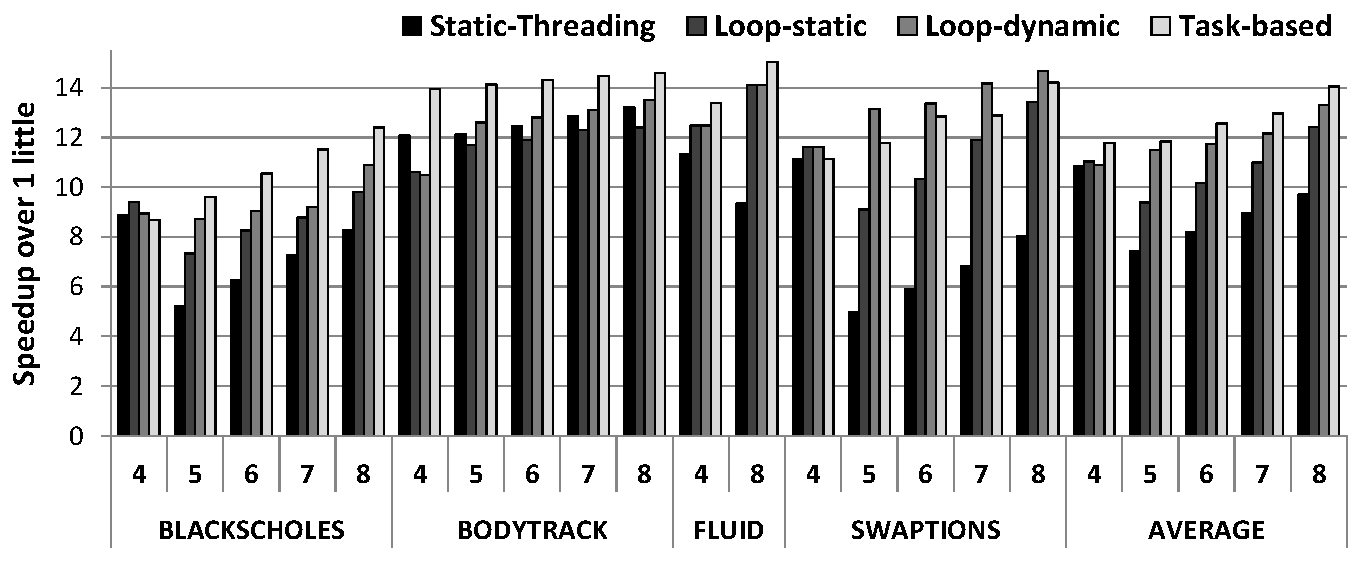
\includegraphics[width=\columnwidth]{figures/speedup-ompssVSopenmp}
        \vspace{-0.5cm}
        \caption{Speedup over 1 little core when running on 4 to 8 cores and 4 of them are big. 
Four different programming models are considered: Static threading using \texttt{pthreads}, 
parallel loops with static scheduling (loop static), parallel loops with dynamic scheduling (loop 
dynamic), and a task-based solution with dynamic scheduling (task-based).}%
        \label{fig:prog_models}%
        \vspace{-0.5cm}
\end{figure}

As we saw in the previous section, current implementations of parallel applications are not ready to fully take advantage of an AMC system.
Applications that are statically threaded using the low-level \texttt{pthreads} library usually suffer from load imbalance since their implementations assume that the work has to be equally distributed among the available cores. 
Implementing advanced load balancing schemes, such as
work pools, in \texttt{pthreads} requires a significant development effort.

As an alternative, many parallel applications are implemented using loop-based scheduling with the 
OpenMP \emph{parallel for} directives. 
In this case, the runtime library is in charge of scheduling work to the available threads in the system, either statically or dynamically, as described in Section~\ref{sec:runtime}.

We compare these solutions to the task-based approach evaluated in the previous sections. 
%Our goal is to evaluate the suitability of each programming model for asymmetric multi-cores. 
Figure~\ref{fig:prog_models} shows the results obtained from running blackscholes, bodytrack, fluidanimate and swaptions on all the scheduling models: static threading, static loop scheduling, dynamic loop scheduling and task-based scheduling. 
We chose these applications as they are the only ones implemented using the OpenMP loop directives.
%available in all the programming models under evaluation: \texttt{pthreads}, OpenMP loop directives and OpenMP tasks.

Looking at the average results in Figure~\ref{fig:prog_models}, we can observe that the task-based solution 
achieves the best results when the system is asymmetric. Task-based improves the static 
threading by up to 59\% on 5 cores, while dynamic loop scheduling improves by up to 54\%.
The OpenMP version with static scheduling reaches an average 26\% improvement over the static-threading approach with pthreads.

Taking a closer look to the results we observe that for bodytrack, an application with sophisticated parallelization techniques, static-threading achieves better results than loop-static.
This is because the static-threading implementation contains specific parallelization techniques that cannot be completely expressed using the loop-static method.
The loop-dynamic method improves performance for bodytrack by up to 4\% due to the runtime decisions of the iteration execution, but the optimal solution is offered by the task-based approach that achieves up to 16\% improvement over static-threading, due to the flexibility in expressing irregular parallelization strategies.
  
Blackscholes, fluidanimate and swaptions, consist of independent tasks and are a good fit for loop parallelism. 
The first observation is that both applications benefit from the loop-static approach on an SMC with 4 big cores. 
Moreover, the task-based approach is still the optimal for blackscholes and fluidanimate, reaching up to 83\% improvement over static threading for 5 cores, while for swaptions loop-dynamic is the most appropriate, improving the baseline by up to 2.6$\times$.
The difference in the benefits of these applications relies on the task granularity; blackscholes consists of 6400 tasks that are about a hundred times smaller than each one of the 128 tasks of swaptions. 
This shows that loop-dynamic is more efficient on coarse-grained applications.
Finally, fluidanimate, that is also a fine-grained application that consists of 128\,500 tasks, also benefits from the task-based approach. 
For this benchmark, static and dynamic loop scheduling achieve similar performance; this is due to the limited parallelism per parallel region, as the loop-based implementation consists of multiple barriers between small parallel regions, fact that diminishes the effect of dynamic vs static scheduling. 
%Thus, if the loops have a small number of iterations, it makes no difference whether these iterations will be scheduled dynamically or statically as the resulting schedule will be the same.

% AR - this sounds wrong, no runtime activity in OMP static sched iteration distribution - This is because the static-scheduling overheads are inside the optimized OpenMP runtime system instead of the application's code. 


  \iffalse
However, 

The second solution is to transfer the responsibility to the runtime system so it dynamically 
schedules work to different core types based on work progress and core availability. The advantage 
is that the runtime system has knowledge of the application structure and parallel work boundaries 
so it can react with certain level of predictability. We evaluate dynamic scheduling on top of the 
existing work-sharing constructs in the applications with an OpenMP statically-scheduled 
implementation available. This requires code transformation that are straightforward in many cases.

We finally evaluate the impact of using a inherently load-balanced execution model such that of 
task-based programming models. Recent examples~\cite{Ayguade:TPDS2009, OpenMP4.0:Manual2013, 
OmpSs_PPL11, Zuckerman:EXADAPT2011, Bauer.2012.SC, Vandierendonck:PACT2011, Vandierendonck:Hyperq} 
include clauses to specify inter-task dependences and remove most barriers which are the major 
source of load imbalance on AMCs.

Comment new figure: Figure~\ref{fig:prog_models}.
Figure~\ref{fig:prog_models} shows the speedup over one little core of blackscholes, bodytrack and swaptions for task-based and static threading solutions compared to loop scheduling solutions. 
The applications are implemented using the OpenMP 2.0 directives for loop scheduling. 
We compare both dynamic and static loop scheduling and the results show that the task-based approach on average outperforms this programming model.
Bodytrack, that consists of highly sophisticated parallel programming techniques performs better with the task-based model as the freedom of task creation and the specification of dependencies helps on a more efficient implementation. 
On the other hand we can observe different behaviour between the highly parallel benchmarks blackscholes and swaptions.
These two benchmarks consist of independent tasks but they show oppositional benefits in terms of the optimal programming model.
Swaptions consists of 128 tasks each of them taking 100$\times$ more time than the blackscholes tasks. 
Blackscholes on the other hand consists of 6400 tasks. 
So, blacksholes is a more fine grained benchmark that lets the task-based programming model to overcome the overheads and increase performance in return.
The loop scheduling work better when the number of tasks is limited and the parallelization is regular.
\fi

%%%%%%%%%%%%%%%%%%%%%%%%%%%%%%%%%%%%%%%%%%
%%%%%%%%%%%%%%%%%%%%%%%%%%%%%%%%%%%%%%%%%%
\if 0 
\subsection{Power Consumption Analysis over Time}

%To understand in detail some of the behaviours pointed out in the last sections, we provide detailed power measurements during the whole execution of the streamcluster benchmark. 

This section provides a detailed analysis of the power consumption over time for one of the evaluated applications, streamcluster.
We choose this application as an illustrative example of the utilization of the processor resources 
(performance and power) with the different evaluated approaches.
Figure~\ref{fig:streamcluster_consumption_evolution} shows the power samples measured over the 
execution time of streamcluster when running on 8 cores (\texttt{4+4} configuration).
On the left part of the figure we plot the power samples of only the 4 big cores, while on the right part we plot the total power samples of all the big and the little cores.
Both charts contain this information for the three scheduling approaches evaluated in this paper (\emph{Static threading}, \emph{GTS} and \emph{Task-based}).
As expected, all the approaches display the same five execution phases throughout the execution, as this benchmark is processing five large chunks of points.
Seemingly the power samples of the big-core cluster slightly outreach 3W for the \emph{GTS} and \emph{Task-based} approaches, while for \emph{Static threading} they remain close to 1.5W. As shown in Figure~\ref{fig:power4}, steamcluster dissipates 1.2W when running on 4 little cores.
Thus, this proves that the \emph{GTS} and \emph{Task-based} approaches better utilize the big cores and, in contrast, the big cores remain idle for a significant amount of time with the \emph{Static threading} strategy.

On the right of Figure~\ref{fig:streamcluster_consumption_evolution}, where the power samples of the whole chip are plotted, the \emph{Task-based} approach has power samples slightly higher than the \emph{GTS} approach:
with the \emph{Task-based} approach, measured power is around 4.0W, while with \emph{GTS} observed power is around 3.6W.
The main difference between these measurements and the ones on the left chart of the same figure is the power consumption of the little cores. 
Thus we derive that both \emph{GTS} and \emph{Task-based} fully utilize the big cores in the system, but the \emph{Task-based} approach utilizes the little cores better than \emph{GTS}. In contrast, \emph{Static threading} does not take advantage of the computational power of this AMC for the streamcluster benchmark.

Despite the fact that performance and power consumption of the little cores are much smaller than the ones of the big cores, the \emph{Task-based} approach significantly reduces the execution time of streamcluster from 374 seconds to 312 seconds. A more effective usage of the little cores at the cost of slightly higher power consumption leads to these results. This clearly demonstrates the benefits of runtime system-based programming models against thread-based approaches in AMC systems.
\fi
%fully using the little cores is extremely important since the task-based approach reduces execution time from 374 to 312 
%without spending much more power by fully exploiting the little cores.


%Figure~\ref{fig:streamcluster_consumption_evolution} contains the measured power consumption per time when streamcluster runs on the 8 cores of the octodroid platform.
%On the left of figure~\ref{fig:streamcluster_consumption_evolution}, we can see the power consumption of just the big cores and on the right the consumption of the whole chip.
%\mc{We need to understand and explain the power dissipation of what hw components (private caches, cores, ...) is being measured.}
%Measurements are shown for the three parallel strategies considered in this paper: \emph{Static Threading}, \emph{GTS} and \emph{task-based}.
%Interestingly, the three considered strategies display the same 5 execution phases, which is obviously expected.
%In terms of power consumption of just the big cores, we can see how these cores dissipate slightly more than 3 Watts when run streamcluster either with the \emph{GTS} or the \emph{Task-based} approaches.
%The \emph{Static threading} approach makes the big cores to dissipate much less power, around 1.5 Watts. 


%This means that the GTS and the task-based approaches use extensively the big cores and, in contrast, the big cores spend a significant amount of idle time under the static threading regime.

%Right of Figure~\ref{fig:streamcluster_consumption_evolution} shows the power consumption when the whole chip is measured.
%In this scenario, things slightly change since the task-based approach spends more power (around 4 Watts most of the time) than the GTS technique (around 3.6 Watts).

%Since the only difference between these measurements and the ones on top of Figure~\ref{fig:streamcluster_consumption_evolution} is the power consumption of the little cores, we can derive that
%the task-based approach uses the little cores much more intensely than the GTS policy, since these cores dissipate much more
%power under the task-based regime than the GTS one. 


%Despite the fact that performance and power consumption of the little cores are much smaller than the ones of the big cores, fully using the little cores is extremely important since the task-based approach reduces execution time from 374 to 312 without spending much more power by fully exploiting the little cores. 

%These results clearly demonstrate the benefits of task-based programming models against thread-based approaches in asymmetric multi-core systems.



%%%%%%%%%%%%%%%%%%%
%%%%%%%%%%%%%%%%%%%
\section{Conclusions}
\label{sec:conclusions}
In this extensive evaluation of highly parallel applications on an ARM big.LITTLE AMC system 
%Our findings include the system's behaviour when modifying the asymmetry level as well as changing the scheduling scheme.
%These results are explained along with the application characteristics which gives another dimension to this study.
we showed that current implementations of parallel applications using pthreads are not ready to fully utilize an AMC.
Implementing highly sophisticated parallelization strategies such as parallel pipelines (ferret) to exploit AMCs at the application level requires a significant programming effort and is not applicable to all workloads.
The built-in GTS heterogeneity-aware OS scheduler only partially mitigates the slowdown of static threading when using both big and little cores.
%Dynamically-scheduled loops achieve better results by distributing the load as iteration chunks. A task-based implementation of the applications achieves even better results by removing barrier synchronizations in many cases.
%When adding little cores to a homogeneous system with big cores we showed that scheduling at the application or at the OS level is not able to always utilize the additional little cores. 
%Contrarily, the task-based approach, due to the dynamic and fine grained scheduling, manages to evenly divide the work to the asymmetric resources.
Both dynamically-scheduled loop- and task-based versions achieve higher performance with increased utilization which results in increased power. This leads to similar energy consumption as static threading and GTS, which ends up with better results in EDP.
%In terms of power, the task-based approach keeps the power dissipation stable even if we add little cores to the system, while at the same time performance is increased. 
%We consider that this is the idea behind such AMC systems and this is a proof that the task-based approach achieves this goal overcoming the GTS scheme.
%In terms of energy, there is some room for improvement on the task-based approach as on average it consumes approximately 3\% more energy than GTS and 5\% more than static threading on 8 cores.
%However, the EDP results show that the optimal solution when taking into account both energy and performance is the task-based. 

Overall, GTS and static threading are not suitable solutions to run intensive multithreaded applications on AMCs. Dynamic scheduling is essential to distribute the load across different core types. A loop-based implementation with dynamic scheduling is appropriate when the parallel work granularity is large and the potential imbalance at the tail of the loop is insignificant compared to the overall parallel region duration. A task-based implementation with inter-task dependencies allows removing barriers, which is the preferred solution, especially when the granularity of parallel regions is small.

%Finally, we further explored the available runtime scheduling options.
%We compared the performance of the task-based approach with two types of loop-based scheduling: static and dynamic. 
%From our available loop-scheduled applications we can conclude that the loop-dynamic approach can outperform task-based only in the case of coarse grained applications. 
%For applications that consist of a very high number of small tasks (blackscholes) or with intensive dependencies between them (bodytrack) the task-based approach is the optimal solution. 



\iffalse 
%removing conclusion of hpca and rewriting it...
AMCs are a successful architectural solution for mobile and supercomputing systems. 
Our evaluation shows how they perform for other domains and how the several existing execution models for AMCs behave in terms of performance and power. 

We compared the statically-threaded out-of-the-box implementation, the GTS OS scheduler, and dynamic scheduling at the runtime level, both for OpenMP loops and a task-based implementation. 
When using all the cores in the system, it stands out that the task-based better balances the load and avoids having big cores waiting for little cores to reach synchronization points.

We confirm that the out-of-the-box implementation, for most applications, does not effectively utilize the asymmetric system.
%does not work for most applications. 
This confirms the well-known problem of load imbalance when evenly distributing work among diverging core types. 
On average, static threading, when using eight cores, is 12\% less efficient than when using just four big cores.
%performs 12\% worse will all cores than with just big cores.
An exception is the case of ferret, due to its pipelined parallelism that helps on the effective utilization of the little cores when they are added to the system.
%makes the
%addition of little cores to provide additional throughput without imbalances.

The OS scheduler partially increases load balance. 
However, as it migrates threads based on CPU utilization, its behaviour is mostly reactive. 
It migrates threads when they become inactive and, at that point, the thread has already been spinning for some time. 
Using all cores in the system is 5\% better than using big cores only.

Finally, using dynamic scheduling on OpenMP work-sharing constructs reduces load imbalance and helps to better exploit all resources.
Task-based parallelism further reduces imbalance achieving 13\% performance uplift with all cores. 
The fundamental factors for this improvement are the removal of fork-join schemes and barriers
thanks to inter-task dependencies.

These solutions provide different levels of application refactoring. 
Our performance and power discussion and quantification becomes a useful resource to select the right execution model for a given performance-effort point and satisfactorily exploit AMCs. 
\fi
%In this paper we examine the maturity of asymmetric multi-core systems to support emerging parallel applications, showing an extensive and comprehensive evaluation in terms of performance, power, energy and EDP. We compare three major scheduling approaches each of them taking place at a different level of the software stack: \emph{Static threading} for application-level parallelism, \emph{GTS} for OS level parallelism, and \emph{Task-based} that takes place at the runtime level.

%An interesting finding of this work is that out-of-the-box emerging parallel applications are not ready to exploit the energy efficient features of asymmetric multi-cores. Many applications assume that the underlying hardware will be symmetric and suffer from load imbalance in the presence of asymmetry. Only applications that implement advanced load balancing techniques can benefit from the enhanced performance and energy efficiency of these systems.
%
%A second important finding of this work is that, depending on the target metric that we want to achieve, asymmetric multi-cores offer different possibilities and tradeoffs. In a system with four \emph{big} and four \emph{little} cores, we evaluated seven different combinations of cores with the described three different scheduling policies, achieving the following conclusions:
%\begin{itemize}
% \item In terms of \emph{power}, the best solution is to use a symmetric configuration with only little cores, as they dissipate much less power than the big cores.
% \item In terms of \emph{performance}, if the system software stack does not provide a dynamic scheduler at some level, the best solution is to use the symmetric multi-core with four big cores. However, if a dynamic scheduler is available at application, runtime or OS level, the best configuration turns to be the asymmetric multi-core with four big and four little cores. The runtime system approach delivers the highest performance in this configuration, reaching a 13\% improvement over the symmetric configuration.
% \item In terms of \emph{energy}, the best configuration is again a symmetric multi-core with four little cores. The enhanced performance that big cores deliver does not compensate the extra power they dissipate.
% \item Finally, in terms of \emph{energy-efficiency}, we show that the best EDP results are obtained in the asymmetric configuration with four big and four little cores and the dynamic scheduler in the runtime system.
%\end{itemize}
%To conclude, in energy-limited environments, it is clear that a multi-core with only little cores is the best solution. However, if we want to reach higher performance and energy efficiency, asymmetric multi-cores offer an interesting solution when combined with a dynamic scheduler in the runtime system.


% \textbf{Kallia:: First draft}
% In this paper we examined the maturity of the asymmetric systems to support emerging parallel applications in terms of performance, energy and power.
% We compared three major scheduling approaches each of them taking place at a different level of the software stack: \emph{Static threading} for application-level parallelism, \emph{GTS} for operating system level parallelism and \emph{Task-based} that takes place at runtime level.
% Moreover, we investigated seven different combinations of big and little cores and we showed the impact of adding little cores on a homogeneous system with big cores.
% Finally, we presented a detailed power analysis of streamcluster and an evaluation of the three possibilities regarding the main thread migration on a task-based programming model.
% 
% Our conclusions can be summarized in two cases; 
% first, is the conclusions for a constant number of cores, and then the conclusions for an increasing number of cores.
% For a static number of cores, the most efficient configuration in terms of performance, would be a homogeneous system with big cores.
% On the other hand, a homogeneous system with little cores would be the most energy efficient set-up of the system.
% For these homogeneous systems all the approaches achieve the same performance.
% If we introduce asymmetry and we make half of the cores big and half of them little, the optimal way to perform scheduling is the \emph{Task-based} approach, due to the dynamic fine-grained parallelism. 
% At the same time this approach is the less energy efficient one on the asymmetric system.
% However, if we take into account performance and energy consumption (namely EDP results) the best combination of the two is given by the use of the \emph{Task-based} approach.
% 
% The second part of the results of this paper focuses on the efficient utilization of the little cores.
% Specifically, we explored the performance, energy, power and EDP improvements when adding four little cores on a system that initially consists of four big cores.
% We observed that the \emph{Static threading} approach fails to efficiently utilize the assistant-little cores since the available parallelized applications assume a homogeneous system and divide the workload on equal units.
% The \emph{GTS} and \emph{Task-based} approaches take more advantage of the little cores since their dynamic approach is more flexible.
% As the \emph{Task-based} approach works on tasks rather than threads (compared to \emph{GTS}) it provides higher flexibility, thus it achieves an additional 10\% performance over \emph{GTS}.
% All the approaches manage to reduce total energy while keeping the power constant.
% Taking into account both energy and performance (EDP), the optimal approach is the \emph{Task-based} and the most efficient system configuration is when adding four little cores to the homogeneous system with four big cores. 
% 
% From the power analysis, we found that the \emph{Task-based} approach utilizes the little cores better than \emph{GTS} and both of them use little cores in a higher intensity than the \emph{Static threading}.
% In the last part we showed that for a task-based programming model the effect of changing the migration of the main thread makes only slight differences and this slight improvements of slowdowns are mostly application-specific.
% On average all the main thread migration options achieve the same results.

\iffalse


Our findings answer these questions:
1. which is the best configuration of big/little cores
-for performance?
-for power?
-for both?
2. which scheduling approach is the best?
3. where should the main thread migrate?



The advantages of asymmetric multi-cores for mobile applications have been proved in the past. 
In this paper, we showed that these systems can also be useful for emerging parallel applications and evaluated three possible ways of utilizing them. 
We found that for a constant number of four cores, the most efficient configuration in terms of performance, power and energy is a homogeneous system consisted of big cores.

If the number of cores remains constant, the best configuration in terms of performance, power and energy is always homogeneous. 
However, asymmetric configurations offer an intermediate solution that can be interesting in some scenarios. Furthermore, if the number of big cores remains constant, having an increasing number of little cores in an asymmetric multi-core can help increasing performance while reducing final energy. 

However, more advanced techniques are required at the application, runtime or OS levels to balance the load across all cores and fully exploit the available resources. Relying on the programmer to develop an application that adapts to asymmetric multi-cores complicates the design and deployment of the application. For this reason, many current parallel applications do not adapt well to these systems. OS-based dynamic schedulers can help mitigating the problems of such applications. However, our results suggest that it is critical to use a flexible parallel programming model to allow the runtime system layer to make decisions dynamically. Having application-agnostic mechanisms to properly balance the load or to perform heterogeneity-aware domain decomposition (i. e. assign more load to more powerful hardware components), allows to fully exploit the potential of asymmetric multi-core processors.

When applying these techniques, average performance benefits of XX\% are obtained, with XX\% reduction in final energy consumption. Taking into account these results, we envision that future desktop and server processors will incorporate heterogeneous cores in their designs.


% Also, all these optimizations must be carried out without increasing the programming complexity as our techniques would be hardly applicable otherwise.
% The runtime system has the responsibility of optimally mapping the tasks to the available cores taking into account hardware components' heterogeneity and availability.

\fi


%\bibliographystyle{elsarticle-num} 
%\section*{References}
%5\bibliography{references}


%\chapter{Task-based Scheduling Solutions}
\chapter{Task-Based Scheduling Solutions}
%%%%%%%%%%%%%%%%%%%
%%%%%%%%%%%%%%%%%%%
\section{Introduction}
\label{sec:intro}
%Too generig... this should be in the main introduction
%The use of asymmetric multi-core architectures forms an appealing solution in high-performance computing to tackle the power wall.
%These architectures increase energy efficiency~\cite{Fedorova2009,Greenhalgh2011,Casas2015} by featuring different types of processing cores designed to target performance or power optimization.

\section{Introduction}
\label{sec.scheduling.intro}

To effectively utilize AMC systems taking into account their heterogeneity, load balancing and scheduling become two of the main challenges~\cite{Li4}.
An approach towards these challenges is the use of task-based programming models~\cite{OmpSs_PPL11,OpenMP,StarSs,starpu}.
The modern task-based programming models schedule tasks dynamically according to the availability of resources. They also allow the specification of dependencies between tasks, enabling the runtime system to automatically perform scheduling and synchronization decisions.

Even though task-based programming models is a powerful mechanism, the efficient mapping of ready tasks to different types of cores on an asymmetric system remains a challenge when considering the reduction of the total execution time. 
Task-based parallel applications expose different characteristics that can affect the total application duration such as complex task dependency graphs (TDGs) with long critical paths or different levels of task cost variability.
In such cases it is very common that the tasks in the critical path determine the total application duration. 
These characteristics influence researchers to develop smart scheduling techniques within a task-based programming model and accelerate the overall application.
%This opens an opportunity to accelerate the overall application 
The criticality-aware schedulers detect the critical tasks of an application and increase performance by running critical tasks on fast cores. 
Some previous works~\cite{DCPS, LDCP, HEFT, CrPathDup} tackled this issue using static scheduling over the whole TDG to statically map tasks to processors on a heterogeneous system. 
However, they required the knowledge of profiling information and most of them were evaluated on synthetic randomly-generated TDGs. 
%More recent works~\cite{Chronaki:ICS2015} tackle this issue through dynamic task scheduling.

%However, there are no previous works on exploring this possibility in a dynamically scheduled environment.

%There are previous works~\cite{xx} on scheduling of task-based applications onto heterogeneous systems. Their approach is to schedule tasks in the critical path to fast cores but all of them target statically-scheduled applications.

This chapter presents three novel dynamic task schedulers that detect the critical path of the in-flight dynamic snapshot of the TDG. 
Furthermore, this chapter shows the potential of the proposed dynamic scheduling techniques compared to a state-of-the-art dynamic heterogeneous scheduler~\cite{HEFT}.
Specifically we compare our approaches against the a dynamic implementation of the heterogeneous earliest finish time scheduler (HEFT)~\cite{HEFT}.
We implement these scheduling policies in the OmpSs~\cite{OmpSs_PPL11,OmpSs} programming model that supports dynamic scheduling and dependency tracking as described in Section~\ref{sec.background.taskbased}.


%we make a study of the potential of dynamic task scheduling techniques such as the criticality aware task scheduler (CATS)~\cite{Chronaki:ICS2015} and a dynamic implementation of the heterogeneous earliest finish time scheduler (HEFT)~\cite{HEFT} as well as we propose two novel dynamic task schedulers that detect the critical path of the task dependency graph.

%propose a criticality-aware \textit{dynamic} task scheduler that dynamically assigns critical tasks to fast cores to improve performance in a heterogeneous system with fast and slow cores. Compared to previous proposals, this scheduler is based on information discoverable at runtime, is implementable and works without the need of an oracle or profiling. Furthermore, our evaluation is based on a real heterogeneous multi-core platform with real applications and, therefore, using real TDGs.
Compared to previous works, all the scheduling policies described and evaluated in this chapter are based on information discoverable at runtime, are implementable and work on a real asymmetric multi-core platform with real applications and therefore, using real TDGs.
The contributions of this chapter are the following: 
\begin{itemize}
 \item{The Criticality-Aware Task Scheduler (CATS) that dynamically assigns critical tasks to fast cores in an AMC system. Tasks are defined to be critical if they are part of the \textit{longest path} in the in-flight dynamic state of the dependency graph. The flexibility and work stealing policy of this scheduler are configurable. Flexibility increases the number of tasks considered critical. Work stealing may be uni- or bi-directional: only fast cores can steal from slow cores, or slow cores can also steal from fast cores.}
 \item{The Critical Path scheduler (CPATH) that dynamically assigns the tasks that belong to the \textit{critical path} of the TDG to the fast cores of the system. To do so, CPATH tracks the execution time of the tasks, assigns cost-based priorities and, according to these priorities it detects the critical tasks.}
 \item{The Hybrid Criticality scheduler (HYBRID) that incorporates the features of CATS and CPATH by assigning to the fast cores tasks that belong \textit{either to the critical path or to the longest path} of the TDG, depending on the runtime circumstances. HYBRID uses mixed priorities that are cost-based or level-based. This technique also keeps track of the task costs but if this information is not available it uses the mechanisms of CATS that dynamically detects the longest dependency chain of the in-flight dynamic state of the TDG}
 
% Two novel critical path based task schedulers that dynamically assign the tasks that belong to the critical path to the fast cores in a heterogeneous multi-core. First, is the Critical Path scheduler (CPATH scheduler) that keeps track of the task costs and discovers the critical path of the TDG according to these costs. In addition, the Hybrid criticality scheduler (HYBRID) also keeps track of the task costs but if this information is not available it uses the mechanisms of CATS~\cite{Chronaki:ICS2015} that dynamically detects the longest dependency chain of the in-flight dynamic state of the dependency graph.}
 % \item{A novel criticality-aware task scheduler (CATS) that dynamically assigns critical tasks to fast cores in a heterogeneous multi-core. Tasks are defined to be critical if they are part of the longest path in the in-flight dynamic state of the dependency graph. The flexibility and work stealing policy of our scheduler are configurable. Flexibility increases the number of tasks considered critical. Work stealing may be uni- or bi-directional: only fast cores can steal from slow cores, or slow cores can also steal from fast cores.}
 \item{An evaluation of CATS, CPATH and HYBRID schedulers compared to the state of the art heterogeneous scheduler HEFT~\cite{HEFT}, all of them implemented in the OmpSs programming model. Moreover we evaluate these approaches next to the default FIFO scheduler that serves as our baseline.
%We use five scientific benchmarks and we perform our experiments on an Odroid-XU3 development board that features an eight-core Samsung Exynos 5422 chip with ARM big.LITTLE architecture including four Cortex-A15 and four Cortex-A7 cores.
%In addition, our evaluation contains the results on simulated heterogeneous systems that consist of 16 or 32 cores. 
The results show that all heterogeneous schedulers improve overall performance reaching up to 45\% improvement. Furthermore, we describe their features such as the high per-task overheads of CPATH, the inability of dHEFT to improve performance when the task number increases as well as the benefit of HYBRID scheduler compared to CATS when task cost variability increases.
}

% An evaluation of a set of heterogeneous schedulers implemented in the OmpSs programming model and the default OmpSs scheduler. Specifically, we use four heterogeneous schedulers: CATS~\cite{Chronaki:ICS2015}, dHEFT, that is a dynamic implementation of HEFT scheduler~\cite{HEFT}, CPATH, which is the Critical-Path scheduling algorithm proposed in this paper, HYBRID, the second heterogeneous scheduling proposal presented in this paper that uses HYBRID criticality of tasks and BF, which is the default OmpSs scheduler and is used as our baseline. We evaluate the effectiveness of these approaches on different numbers of cores and shares of fast and slow cores on an Odroid-XU3 development board featuring an eight-core Samsung Exynos 5422 chip with ARM big.LITTLE architecture including four Cortex-A15 and four Cortex-A7 cores. We also evaluate the effectiveness of these approaches on larger heterogeneous systems of 16 and 32 cores using simulation. The results show that all heterogeneous schedulers improve overall performance reaching up to 45\% improvement. However we describe their features such as the high per-task overheads of CPATH, the inability of dHEFT to improve performance when the task number increases as well as the benefit of HYBRID scheduler compared to CATS when task cost variability increases.}
 
 %The results show that CATS constantly improves overall performance reaching up to 38\% improvement over the baseline. Moreover, dHEFT also improves the baseline by up to 45\% but the results show that by increasing the number of tasks, the performance of dHEFT decreases. The CPATH scheduler, struggles to improve the baseline by up to 23\% due to the increased per task overheads during the critical path exploration process. Finally, HYBRID 
 
% and in some cases HYBRID scheduler outperforms CATS showing improvement of 17\%. On the other hand, CPATH scheduler suffers }

% \item{An evaluation of our implementation of CATS in the OmpSs programming model compared to a dynamic implementation of Heterogeneous Earliest Finish Time \cite{HEFT} and the default OmpSs scheduler. We evaluate the effectiveness of CATS on different numbers of cores and shares of fast and slow cores on an Odroid-XU3 development board featuring an eight-core Samsung Exynos 5422 chip with ARM big.LITTLE architecture including four Cortex-A15 and four Cortex-A7 cores. We also evaluate the effectiveness of CATS on different speed ratios between fast and slow cores using simulation of heterogeneous multi-cores with up to 128 cores. The results show that CATS improves overall performance up to 1.3$\times$ on the real eight-core platform, and up to 2.7$\times$ on a simulated 128-core~system.}
\end{itemize}
Table~\ref{tab.acronyms} shows the acronyms that we use in the next sections.
% We describe a set of configurations for our scheduler regarding the work stealing capabilities of the different core types and the flexibility to define a task as critical or non-critical. 
 
% We implement this scheduler in OmpSs and evaluate its effectiveness on different numbers of cores and shares of fast and slow cores on a real system. 
 
% We also evaluate the effectiveness of our scheduler depending on the speed ratio between fast and slow cores using simulation.  The results show that the effectiveness of our scheduler increases with larger numbers of fast cores over slow cores, and with larger differences of performance between fast and slow cores.

%Finally, we provide a set of recommendations on how to configure our scheduler to get the best results depending on the target system size and configuration.
\begin{table}
\begin{center}
\caption{Acronyms used in the paper \kc{Move all acronyms at the beginning of the thesis? Or remove them totally?}}
\label{tab.acronyms}
\begin{tabular}{|c|c|}
\hline
 \textbf{Acronym} & \textbf{Meaning}\\\hline\hline
TDG & Task Dependency Graph \\
CATS & Criticality-Aware Task Scheduler\\
CPATH & Critical Path-Aware Scheduler\\
HEFT & Heterogeneous Earliest Finish Time\\
dHEFT & Dynamic Heterogeneous Earliest Finish Time\\
BF & Breadth-First\\
HYBRID & Hybrid Criticality-Aware Scheduler\\
FIFO & First-In First-Out\\
\texttt{plist} & Predecessors' List\\
\texttt{slist} & Successors' List\\
tt-is & Task Type - Input Size\\
\hline
\end{tabular} 
\end{center}
\vspace{-0.4cm}
\end{table}


%%%%%%%%%%%%%%%%%%%
%%%%%%%%%%%%%%%%%%%
\section{Background}
\label{sec:background}\label{sec:suitability}
The OmpSs programming model is a task-based programming model that offers a high level abstraction to the implementation of parallel applications for various homogeneous and heterogeneous architectures~\cite{OmpSs_PPL11,OmpSs}. It enables the annotation of function declarations with the task directive, which declares a task. Every invocation of such a function creates a task that is executed concurrently with other tasks or parallel loops. OmpSs also supports task dependencies and dependency tracking mechanisms~\cite{StarSs}. OmpSs is built with the support of the Mercurium compiler, responsible for the translation of the OmpSs annotation clauses to source code, and the Nanos++ runtime system, responsible for the internal creation and execution of the tasks.

%As a task-based parallel programming model, OmpSs enables the annotation of function declarations with the task directive. If a function is declared as a task, then every invocation of this function creates a task that is executed concurrently with other tasks or parallel loops. The accessible data to each task are the arguments of the function. OmpSs uses the StarSs~\cite{StarSs} dependency tracking mechanisms and each task may be annotated with the \textit{in}, \textit{out}, \textit{inout} clauses. These clauses allow the specification of scalars, arrays and pointers as input, output or input and output data of a task. The implementation of a barrier is supported under the \textit{taskwait} clause, and it can also be used with the addition of the \textit{on} clause, to declare a barrier for the group of tasks that produce a specific piece of data. These original OmpSs features can now be found in OpenMP 4.0~\cite{OpenMP}.

Nanos++ is an environment that serves as the runtime platform of OmpSs. It provides device support for heterogeneity and includes different plug-ins for implementations of schedulers, throttling policies, barriers, dependency tracking mechanisms, work-sharing and instrumentation. This design allows to maintain the runtime features by adding or removing plug-ins, facilitating the implementation of a new scheduler, or the support of a new architecture.

The implementations of the different scheduling policies in Nanos++ perform various actions on the states of the tasks. A task is \textit{created} if a call to this task is discovered but it is waiting until all its inputs are produced by previous tasks. When all the input dependencies are satisfied, the task becomes \textit{ready}. The ready tasks of the application at a given point in time are inserted in the \textit{ready queues} as stated by the scheduling policy. Ready queues can be thread-private or shared among threads. When a thread becomes idle, the scheduling policy picks a task from the ready queues for that thread to execute. The default OmpSs scheduler employs a \textit{breadth-first} policy~(BF)~\cite{Duran_schedulers_08} and implements a single first-in-first-out ready queue shared among all threads. When a task is ready, it is inserted in the tail of the ready queue and when a core becomes available, it retrieves a task from the head of the queue. BF does not differentiate among core types and assigns tasks in a first-come-first-served basis. We use this scheduler as our baseline.

The Nanos++ internal data structures support task prioritization. The task priority is an integer field inside the task descriptor that rates the importance of the task. If the scheduling policy supports priorities, the ready queues are implemented as \textit{priority queues}. In a priority queue, tasks are sorted in a decreasing order of their priority. The insertion in a priority queue is always ordered and the removal of a task is always from the head of the queue, i.e., the task with the highest priority. The priority of a task can be either set in user code, by using the \textit{priority} clause, which accepts an integer priority value or expression, or dynamically  by the scheduling policy, as is described in the next section.

%The default OmpSs scheduler employs a \textit{breadth-first} policy~(BF)~\cite{Duran_schedulers_08}. The BF scheduler implements a single first-in-first-out ready queue shared among all threads. When a task is ready, it is inserted in the tail of the ready queue and when a core becomes available, it retrieves a task from the head of the queue. Tasks are ordered according to their ready time: the earliest ready task resides at the head of the queue. Since the ready queue is shared, there is no need for work stealing and the load is balanced automatically. BF does not differentiate among core types and assigns tasks in a first-come-first-served basis. We use this scheduler as a baseline for the evaluation.

%%%%%%%%%%%%%%%%%%%
%%%%%%%%%%%%%%%%%%%
\section{Heterogeneous Scheduling}
\label{sec:scheduling}
The efficient scheduling problem has been intensively studied for asymmetric systems.
In this section we describe four scheduling approaches that target such systems.
The first three are based on separating the tasks into groups of critical and non-critical tasks and assign each group to one core type: the critical tasks to the fast cores and the non-critical tasks to the slow cores.
The difference between these three approaches is the way of considering a task critical.
First is the Criticality-Aware scheduler (CATS)\cite{Chronaki:ICS2015}, which detects the critical tasks based on their \textit{bottom level}.
Secondly, the Critical Path scheduler (CPATH), proposed in this paper, that detects the critical path of the dynamic (TDG) with the help of \textit{bottom cost} based priorities.
The Hybrid Criticality scheduler (HYBRID), proposed in this paper, uses both bottom level and bottom cost based priorities.
Last, we describe a dynamic implementation of HEFT scheduler (dHEFT)~\cite{HEFT}, that for every task it detects the processor that finishes its execution at the earliest possible time.
All of the described schedulers operate at runtime on the dynamic snapshots of the TDG. 
CPATH, HYBRID and dHEFT perform on-line profiling of the task execution time without considering inter-task communication costs, given the uncertainty of data movement latency that hides in the cache hierarchy of an asymmetric multi-core system with prefetching. 
%but none of these schedulers track the inter-task communication costs.


\lstset{basicstyle=\footnotesize\ttfamily,
        emphstyle=\bfseries,
        columns=fixed,
        numbers=none,
        moredelim=*[l][\textit]{//},
        moredelim=*[l][\bfseries]{\#},
        literate={...}{\dots}3
} 
\subsection{Criticality-Aware Task Scheduler}
\label{sec.cats}
The Criticality-Aware Task Scheduling generally applies to task-based programming models supporting task dependencies, but for simplicity we explain it in the context of the OmpSs programming model.
CATS uses bottom-level longest-path priorities and consists of three steps:
%\begin{itemize}

\textbf{Task prioritization}: when a task is created and added to the TDG, it is assigned a priority and the priority of the rest of tasks in the graph is updated accordingly.
 %Since the task graph is generated at runtime, there is no way to statically compute the priority that will be given to a task. 

\textbf{Task submission}: when a task becomes \textit{ready}, i.e., all its predecessors finished their execution, it is submitted to a \textit{ready queue}. At this point, the algorithm decides whether the task is considered \textit{critical} or \textit{non critical}. The task is then inserted in the corresponding ready queue: tasks in the \textit{critical ready queue} will be executed by fast cores, and tasks in the \textit{non-critical ready queue} will be executed by slow cores.

\textbf{Task-to-core assignment}: when a core becomes idle, it tries to retrieve a task from its corresponding ready queue to execute it. If the queue is empty, it might try to steal from the other queue according on the work stealing policy. %Currently, we support two work stealing mechanisms: \textit{simple} work stealing, i.e., fast cores can steal from slow cores; and \textit{bidirectional} (\textit{2DS}) work stealing, i.e., both types can steal from the other. The default policy is \textit{simple}.
%\end{itemize}

These steps are performed dynamically and potentially in parallel in different cores. Thus, while some tasks are being prioritized, previously created tasks may be submitted, and others assigned to available cores or executed.

To give an overview of the scheduling process, Figure~\ref{botlevels} shows a scheme of the operation of CATS. In the TDG on the left, each node represents a task and each edge of the graph represents a dependency between two tasks. The number inside each node is the \textit{bottom level} of the task: the length of the longest path in the dependency chains from this node to a leaf node. The priority of a task is given by its bottom level. The pattern-filled nodes indicate tasks that are considered critical. The number outside each node is the task id and is used in the text to refer to each task. Critical tasks are inserted in the critical queue, and non-critical tasks to the non-critical queue. The insertion is ordered with the highest priorities at the head of the queue and the lowest priorities at the tail. Slow cores retrieve tasks from the head of the non-critical queue and fast cores from the critical queue. The following sections describe these scheduling steps in~detail.


\begin{figure}[t]
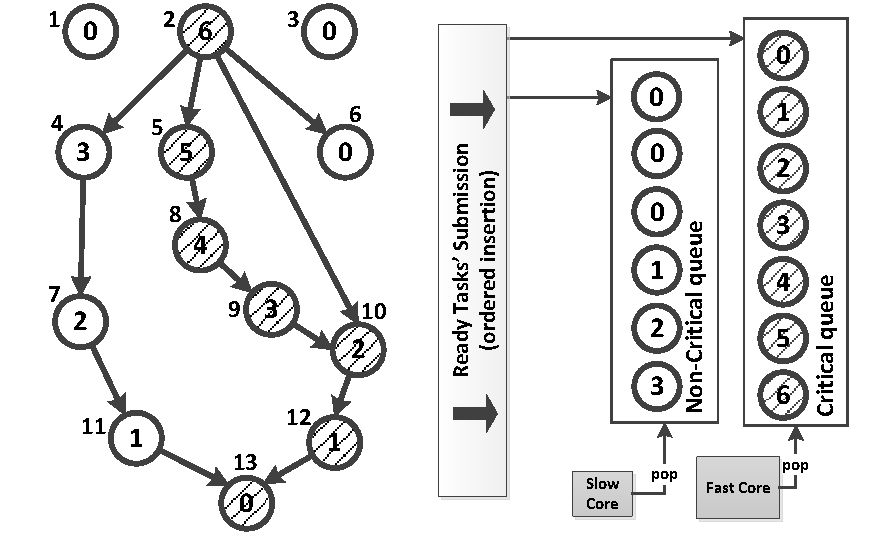
\includegraphics[width=\columnwidth]{images/fig_1.pdf} 
\centering
\caption{Task submission with CATS. Nodes are marked with the \textit{bottom level} of each task. Pattern-filled nodes mark the critical tasks.}
\label{botlevels}
\vspace{-0.5cm}
\end{figure}


\subsubsection{Task Prioritization}

Each task in the TDG has a list to include its predecessors (\textit{plist}). Every time an edge is added into the TDG on the creation of a new task, the corresponding predecessor of the dependency is added in the \textit{plist} of its successor. For example, in Figure~\ref{botlevels}, when the dependency between tasks~2 and~5 occurs, the task number~2 is inserted into the \textit{plist} of the task number~5. Thus, the \textit{plist} of task number~5 becomes $\{$2$\}$. Accordingly, the \textit{plist} of task number~10 will be $\{$2, 9$\}$ when the edge~9$\rightarrow$10 is inserted to the TDG. 

%Right after the occurrence of a dependency between two tasks, the task prioritization step takes place, once for each edge of the graph. 
%represented by the edges in the graph, that connect one predecessor task with one successor task.

The priority given to a task is the \textit{bottom level} of the task. The \textit{bottom level} is computed by traversing the TDG upwards starting from the successor that the currently created edge is pointing to. The priority of this successor is 0 because it is a leaf node of the graph, as it is the last created task. Then, using \textit{plist} for each task, the algorithm navigates to the upper levels of the TDG and updates the priority on each visited node. This way not all the graph is updated, but only the tasks that are predecessors in the paths to the new edge. The algorithm also stops going up through a path, when it finds a priority larger than the one it would be updated to.

Listing~\ref{creation} shows the algorithm for task prioritization. The complexity of this is \textit{O($n^2$)}, \textit{$n$} being the number of tasks. This function is called on the creation of a new edge with the successor as argument. The algorithm traverses the \textit{plist} of the successor task (line 5) and if the priority of the current predecessor is lower than the bottom level of the successor plus one, it updates the current predecessor's priority to that value (lines 7-8). If the updated predecessor task is ready (i.e., it sits in one of the ready queues), the scheduler reorders the ready queue so it remains ordered considering the updated priority (lines 9-10). Then, the same actions are performed recursively for each predecessor of the \textit{plist} to update all the possible upward paths from the successor. 

The terminate conditions for the TDG navigation are two: \textit{(a)} if the \textit{plist} of the current task (\texttt{currPred}) is empty, so either we reach an entry node or the predecessors of the task have finished execution; or \textit{(b)} if the priority of the current task (\texttt{currPred}) remains unchanged, which means that the successor task (\texttt{succ}) does not belong to the longest path because its predecessor already has a higher priority. 
\begin{lstlisting}[float, emph={void,if,return,non_critical_queue, critical_queue,prioritize_task}, captionpos=b, caption={Pseudo-code task prioritization with CATS.},label=creation, emph={[2]mat}, emphstyle={[2]}, aboveskip={0\baselineskip}, frame=tb, belowskip={-0.4cm}]
1 void prioritize_task(task *succ) {
2  int blev = succ->priority;
3  list plist = plistOf(succ);
4  task *currPred;
5  while( not isEmpty(plist) ) {
6    currPred = plist.next();  
7    if(priorityOf(currPred) < blev+1) {
8     currPred->priority = blev+1;
9     if(isReady(currPred)) 
10     readyQueueOf(currPred)->reorder();
11    prioritize_task(currPred);
12   }
13 }
14}
\end{lstlisting}
\subsubsection{Task Submission}

%CATS supports two task submission policies: the \textit{flexible} policy adds more task in the critical queue for the fast cores, while the \textit{strict} policy reduces the number of critical tasks.

The purpose of this step is to divide the tasks into two groups: \textit{critical} and \textit{non-critical}. Critical tasks are tasks that belong to the longest path of the dynamic TDG, namely the path  with the maximum number of tasks (or nodes). Thus, the longest path starts from the task with the maximum bottom level. At runtime, the longest path changes as tasks complete execution and new tasks are created. CATS manages to detect these changes and dynamically decide if the submitted task belongs to the longest path of the TDG.

When a task's dependencies are satisfied, the task becomes ready for execution and is to be inserted in the \textit{ready queues}. Ready queues are priority queues that keep tasks in a decreasing order of task priorities, i.e., the task with the maximum priority resides on the head of the queue. Critical tasks are inserted in the critical queue and non-critical tasks in the non-critical queue. The pattern-filled nodes in Figure~\ref{botlevels} represent the critical tasks in that graph. 

%This way, tasks in the critical queue will then be scheduled to fast cores, and non-critical tasks to slow cores.

%By keeping track of the last discovered critical task%task with the maximum priority
To determine the criticality of a task, CATS keeps track of the last discovered critical task. Then, for each task that becomes ready, CATS checks the following conditions:
%, our approach to detect critical tasks in the graph is to check the following two conditions for each task that becomes ready:
\textit{(a)} if the priority of the current ready task is higher or equal to the priority of the last discovered critical task and, \textit{(b)} if the current ready task is the highest-priority immediate successor of the last discovered critical task.

%%%%%%%%%%%%%%%%%%%%%%%%%%%%%%%%%%%%%%%%
\if 0 %flexible strict explanation
In the first case, the algorithm detects new longest paths that may have been created by the application throughout the execution of a prior longest path. In this case, the scheduler can either be \textit{strict} or \textit{flexible}:
\begin{itemize}
 \item{\textit{Strict}: marks as critical tasks with priority higher than the priority of the last critical task.}
 \item{\textit{Flexible}: marks as critical tasks with priority higher or equal to the priority of the last critical task.} 
 \end{itemize}
As a result, the flexible scheduler ends up with more critical tasks than the strict. The flexibility of the scheduler can be set by the programmer through an environment variable.
\fi % about flexible/strict explanation
%%%%%%%%%%%%%%%%%%%%%%%%%%%%%%%%%%%%%%%%%%%%
\begin{figure}[tl!]
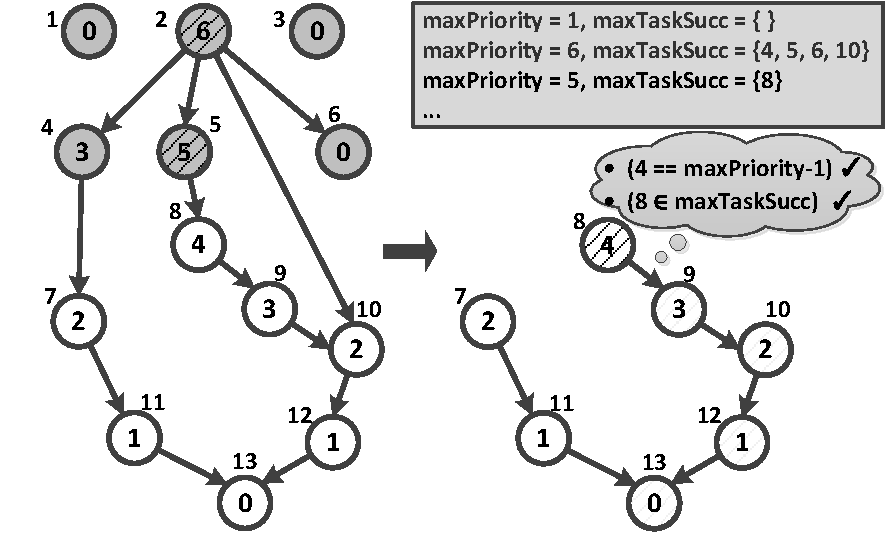
\includegraphics[width=\columnwidth]{images/fig_2.pdf} 
\centering
\caption{Task submission. Gray nodes indicate finished tasks and pattern-filled nodes indicate critical tasks.}
\label{submitFig}
\vspace{-0.5cm}
\end{figure}
The task that satisfies the second condition is a task with a lower priority than the maximum but the task belongs to the longest path because it is the highest priority immediate successor of the last detected critical task. 

Listing~\ref{submission} shows a simplified version of the task submission code, that is of complexity \textit{O($n$)} (\textit{$n$} is the number of tasks). The variable \texttt{maxPriority} (line 1) is used to store the priority of the last critical task, and \texttt{maxPriorityTask} (line 2) is used to store the last critical task. Initially, \texttt{maxPriority} is set to 1 and \texttt{maxPriorityTask} is set to \texttt{NULL}. This avoids the scheduling of independent tasks (i.e., tasks with zero priority) to fast processors at the start of the execution. On the first ready task, if its priority is higher or equal than 1 (line 5) , it is considered to be the first task of the longest path. Therefore, it is inserted in the critical queue and the variables \texttt{maxPriority} and \texttt{maxPriorityTask} are updated accordingly (lines 9-11) to determine correctly the criticality of the next submitted task.

If the priority of the submitted task is equal to \texttt{maxPriority - 1}, we check if it also belongs to the successors of the task with the maximum priority (lines 6-7) and therefore to the longest path. If these two conditions are met, the task is determined to be critical, it is inserted in the critical queue and, as before, the variables \texttt{maxPriority} and \texttt{maxPriorityTask} are updated (lines 9-11). In the rest of the cases the task is not considered critical and it is inserted in the non-critical queue.

Figure~\ref{submitFig} shows an example of a TDG during task submission. The gray nodes in the graph are tasks that have finished execution and the pattern-filled nodes are critical tasks. The numbers inside the nodes indicate their priority and the numbers outside the nodes show the task id, which is assigned in task creation order. The variable \texttt{maxPriority} corresponds to the priority of the last critical task and the \texttt{maxTaskSucc} is the list of the successors of the last critical task, filled with the task ids of the successors. Initially, \texttt{maxPriority} is set to~1 and \texttt{maxTaskSucc} is empty. When task~2 is about to be submitted, it is inserted in the critical queue because its priority is higher than the maximum, which at the beginning is~1. Then, the value of \texttt{maxPriority} is set to~6 (priority of task~2), and the \texttt{maxTaskSucc} list is updated with the successors of task~2. At the point where all the gray tasks have finished execution, the values of \texttt{maxPriority} and \texttt{maxTaskSucc} are updated as shown  in Figure~\ref{submitFig}. For every newly-ready task, the conditions listed above are evaluated. When task~7 is submitted, it is not considered as critical because it does not belong to the \texttt{maxTaskSucc} list and its priority is not equal to \texttt{maxPriority-1}. Contrarily, task 8 satisfies both conditions and so the task is inserted in the critical queue.

\begin{lstlisting}[float, emph={void,if,return,non_critical_queue, critical_queue,submit_task}, captionpos=b, caption={Pseudo-code for task submission with CATS.},label=submission, emph={[2]mat}, emphstyle={[2]}, aboveskip={0\baselineskip}, frame=tb, belowskip={-0.4cm}]
1 int maxPriority = 1;
2 task *maxPriorityTask = NULL;
3
4 void submit_task(task *t) {
5  if( t->priority >= maxPriority or
6     (t->priority == maxPriority-1 and
7      t $\in$ succListOf(maxPriorityTask)) )
8  { //the task is critical
9    critical_queue.push(t);
10   maxPriority = priorityOf(t);
11   maxPriorityTask = t;
12   return;
13 }
14 //the task is non-critical
15 non_critical_queue.push(t);     
16}
\end{lstlisting}

\subsubsection{Task-to-Core Assignment}
\label{sec.cats.assignment}
Task-to-core assignment takes place dynamically and in parallel to the previous steps and its time complexity is \textit{O($n$)}, \textit{$n$} being the number of tasks. When a core becomes idle, it checks the corresponding ready queue (depending on the core type) to get a task to execute. Fast cores retrieve critical tasks from the critical queue, while slow cores retrieve non-critical tasks from the non-critical queue. Each ready queue is shared among the cores of the same type so there is no need for work stealing among cores of the same type. 

If tasks in an application are imbalanced, i.e., the majority are non-critical and only a few tasks are critical, or vice versa, one of the types of processors would be overloaded and the other would starve for work. This can happen in applications with wide graphs and a large amount of tasks, where the ratio between critical tasks and the total amount of tasks may be small. To leverage the resources, the work-stealing mechanism for CATS lets fast cores steal work from slow cores whenever the critical queue becomes empty. 
%Also, CATS can be configured to perform \textit{bidirectional work stealing} so slow processors can also steal tasks from the critical queue if the non-critical queue is empty. 
%We evaluate these different options and show the results in the next section.

\section{Critical Path Scheduler}
\label{sec.scheduling.cpath}
\begin{figure}[tr]
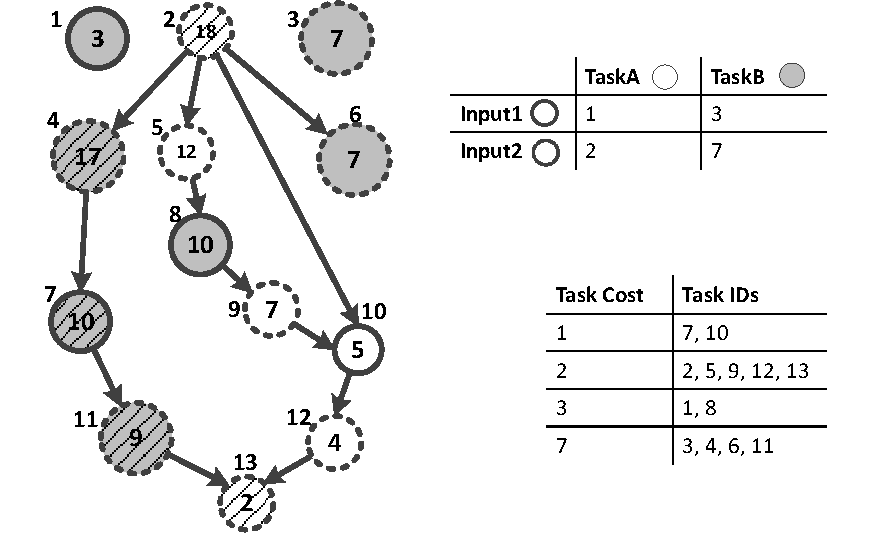
\includegraphics[width=\columnwidth]{images/cpath_priorities.pdf} 
\centering
\caption{Priority assignment taking into account the task costs. Task costs are assumed known and are shown in the tables.}
\label{cpath}
\vspace{-0.5cm}
\end{figure}


The Critical Path scheduler (CPATH) dynamically detects the critical path of the TDG.
Like CATS, CPATH separates tasks into two groups: critical and non-critical tasks.
The detected critical tasks are executed by the fast cores in the system and non-critical tasks are executed by slow cores.
The difference with CATS is the algorithm for critical path detection.
CPATH takes into account the task execution time, about which CATS is unaware.
To do so, CPATH implements a more complex and accurate critical path detection algorithm that takes into account task execution time.

CPATH scheduler consists of three steps:
%\begin{itemize}

\textbf{Task prioritization}: this step takes place when a task is finishing its execution. This is different than CATS since at the end of a task execution the algorithm may record the task execution time (task cost).
%might track a new (unknown) task cost. 
According to the discovered task cost CPATH assigns priorities to tasks by traversing the TDG from top to bottom, introducing the cost of \textit{O($2n^2$)}, where \textit{$n$} is the number of tasks.

\textbf{Task submission}: when a task becomes \textit{ready}, it is submitted to a \textit{ready queue}. At this point, CPATH decides whether or not the task is \textit{critical} and inserts it in the corresponding ready queue. This step has only slight implementation differences with CATS and complexity of \textit{O($n$)}.

\textbf{Task-to-core assignment}: this step is identical to CATS.
% and supports the same work stealing mechanisms.

%\end{itemize}

\subsection{Task Prioritization}
%explanation of the slist (successors' list)

Each task of the TDG keeps a list with its successors (\textit{slist}).
This list is being built when an edge (dependency between two tasks) is added in the TDG.
So when a task dependency occurs, the corresponding successor task is added in the \textit{slist} of its predecessor.
For example, on Figure~\ref{cpath}, when the dependency between tasks 2 and 4 occurs, the \textit{slist} of task number 2 becomes \{4\}. 
This goes on for all the added edges of the TDG, therefore when the edge~2$\rightarrow$5 is inserted in the TDG, the task number 5 is inserted in the \textit{slist} of task number 2; so the \textit{slist} of task number 2 becomes \{4, 5\}.

The goal of this step is to assign priorities based on the \textit{bottom cost} of the tasks of the TDG.
We define the \textit{bottom cost} of a node on a directed acyclic graph as the maximum estimated time in the dependency chains from this node to a leaf node.
So the main difference between the \textit{bottom level} and the \textit{bottom cost} is the consideration of the estimated time.

Figure~\ref{cpath} is used to describe the priority assignment with CPATH.
The specific TDG contains tasks of two different types and two different input sizes.
Node color shows the different task types and the outline of the circle (dashed or solid) shows the different input sizes.
The upper table in Figure~\ref{cpath} indicates the execution time of the tasks according to their type and input size.
The algorithm assumes that task instances of the same type with the same input size have the same (or very similar) execution time.
To track this information, CPATH discovers the cost of every possible task type-input size duple (tt-is duple) that appears on the TDG.
The numbers inside the nodes show the bottom cost-based priorities that CPATH assigns and the numbers outside the nodes show their task ID.


%This task type-input size duple is denoted as tt-is and the algorithm assumes that the task with the same tt-is have the same execution time.
%So the execution time of the tasks differs according to the task type-input size duple (\texttt{tt-is} duple).
%CPATH discovers the cost for all the tt-is pairs and prioritizes the tasks according to their \textit{bottom cost} as shown on Figure~\ref{cpath}.
%The bottom cost of a node is equal to the maximum estimated time in the dependency chains from this node to a leaf node.

The task prioritization step takes place every time a task finishes execution. 
CPATH uses a vector to store task costs and keeps one entry per tt-is.
Because CPATH needs to discover the unbiased critical path of the TDG, it uses one of the core types as reference to track the task costs.
%So at the beginning of the execution tasks are executed on one of the core types during this cost-learning phase.
In our experiments we chose to use as reference the fast cores since this way the learning phase (that is, the phase where CPATH discovers the task costs) becomes shorter.
To avoid wrong task cost prediction of future tasks, CPATH ignores the first execution of each tt-is because usually it takes more time. 
\begin{lstlisting}[float, emph={for,in,void,if,return,updatePriorities,non_critical_queue, critical_queue,submit_task}, captionpos=b, caption={Pseudo-code for taskExit, the function called by the cores used as reference for tracking the task costs},label=cpathExit, emph={[2]mat}, emphstyle={[2]}, aboveskip={0\baselineskip}, frame=tb, belowskip={-0.4cm}]
1 void taskExit (task* finished) {
2  if( stateOf(finished) == init ) {
3    finished->state = in_progress;
4    return;
5  }
6  if( stateOf(finished) == in_progress ) {
7    timesSet[finished] = finished->execTime;
8    finished->state = tracked;
9  }
10 task* succ;
11 for( succ in finished->successors ) 
12   if( numPredecessorsOf(succ) == 1 ) {
13     lock();
14     if( succ $\notin$ entryNodes ) 
15       entryNodes->push(succ);
16       unlock();
17   }
18 list<task>* updatedList = new list<task>();
19 for( node in entryNodes) 
20   updatePriorities(node, updatedList);
21 for( node in updatedList ) 
22    node->unsetUpdated();
23}
\end{lstlisting}

Listings \ref{cpathExit} and \ref{cpathUpdate} show how the critical path scheduler performs task prioritization.
Whenever a task finishes execution on one of the cores used as reference (here: fast cores) the runtime makes a call to the \texttt{taskExit} routine shown in Listing~\ref{cpathExit}.
At this point, the runtime is aware of the execution time of the finished task.
This function has the responsibility to update the known task costs and also perform the prioritization of the tasks on the TDG.
The prioritization is done by the \texttt{updatePriorities} function of Listing~\ref{cpathUpdate}. 
This function is responsible for TDG traversal.

The \texttt{taskExit} function in Listing~\ref{cpathExit} takes as an argument the task that has just finished. 
In order to keep track of whether the execution time of the tt-is has been discovered we implement a small finite state machine within this stage.
Every tt-is has three possible states. 
The initial state is the \texttt{init} state; this means that the specific tt-is has not yet been executed so its execution time is totally unknown.
When a tt-is is executed for the first time its state changes from \texttt{init} to 
\texttt{in$\_$progress}. 
This means that a task of this tt-is has been executed once, but CPATH ignores this cost because the first instance may not be representative due to cold start effects and one sample may not be enough history for prediction.
While the tt-is of a node is in \texttt{init} or \texttt{in$\_$progress} state its execution time is considered to be 1.
%we have to ignore this execution because usually it takes too long and is not representative.
After the second execution of a tt-is the state of it becomes \texttt{tracked} meaning that the execution time has been tracked and can be used for the computation of the priorities.
%If the node does not have a known execution cost tracked, we consider its execution time to be 1.

After the first checks of the tt-is state (lines 2-9 of Listing~\ref{cpathExit}) the algorithm traverses the \textit{slist} of the finished task and searches for the successors that become ready by the end of the execution of this task.
This is identified by the fact that the ready-to-be successors have one unique (remaining) predecessor (e.g. the just finished task).
These successors are inserted in the \texttt{entryNodes} list (lines 11-16 of Listing~\ref{cpathExit}).
For each one of the entry nodes the \texttt{updatePriorities} function is called (line 19 of Listing~\ref{cpathExit}); this performs a top to bottom traversal of the TDG and updates the priorities.

\begin{lstlisting}[float, emph={for,in,void,if,return,non_critical_queue, critical_queue,submit_task}, captionpos=b, caption={Pseudo-code for task prioritization with CPATH},label=cpathUpdate, emph={[2]mat}, emphstyle={[2]}, aboveskip={0\baselineskip}, frame=tb, belowskip={-0.5cm}]
1 int updatePriorities (task* currT, list* updated) {
2   if( currT == NULL )  return 0;
3   if( isVisited(currT) )  
4     return priorityOf(currT);
5   successors = currT->successors;
6   int maxSucc = -1;
7   bool succVisited = true;
8  
9   for(succ in successors) {
10    int succPriority;
11    //Avoid double update
12    if( !isUpdated(succ) || !isVisited(succ) ) {
13      succPriority = updatePriorities(succ, updated);
14      succ->setUpdated();
15      updated->push(succ);
16    }
17    else 
18      succPriority = priorityOf(succ);
19    if(succPriority > maxSucc)
20       maxSucc = succPriority;
21    succVisited = succVisited && isVisited(succ);   
22  }
23  if( timeIsTracked(currT) ) {
24    currT->priority = (maxSucc + timesSet[currT]);
25    if(succVisited && groupOf(currT) < twDetected) 
26      currT->setVisited();
27  }  
28  else
29    currT->priority = maxSucc + 1;
30    
31  return priorityOf(currT);  
32}
\end{lstlisting}

Due to the properties of the top-to-bottom TDG traversal, the algorithm has to make sure that every node is prioritized only once per \texttt{updatePriorities} call.
This is controlled by checking the \texttt{updated} flag of each node of the TDG.
To visualize this situation let us assume that task number 2 of the TDG on Figure~\ref{cpath} finishes.
Then the \texttt{entryNodes} list contains three tasks that will start the update: \{4, 5, 6\}.
The update that starts from task number 4 marks tasks 4, 7, 11 and 13 as updated.
Then, during the update of task number 5, the algorithm knows that task 13 has already been prioritized during the same update so there is no need to apply the algorithm at this node again.
This example does not show too much optimization because in this case the update of only one node is saved, but in real applications this node could have numerous successors for whom the priority update would be a large overhead.

The raising of the \texttt{updated} flag is something temporal and is only used for helping the prioritization of a single update.
There are cases when CPATH needs to raise a permanent flag in order to mark that the priority of the task will not change again in the future, e.g. it is the final priority.
This happens when the execution times of all the tt-is that appear on the TDG have been discovered, for the tasks that their priorities are up to date.
To mark these tasks CPATH uses the \texttt{visited} flag.
If a task is \texttt{visited}, there is no need to get prioritized again.
To clarify this, let us assume that in Figure~\ref{cpath} the task costs of the tt-is TaskA-Input2 and TaskB-Input2 are known.
During the next prioritization, tasks 11 (TaskB-Input2), 12 (TaskA-Input2) and 13 (TaskA-Input2) in the TDG will be set as visited, because their priorities consist of the sum of known task execution times and they do not have any successors (with unknown execution times).
So, an additional priority update in cases like this is redundant.
%So, the algorithm does not need to visit these nodes again on the current update, nor on a future priority update.


%Moreover, CPATH prioritization needs to make sure that the priority of a to-be-updated node is not the final priority.
%In case that the priority of a node is final then there is no need for updating this node.
%To perform this check, CPATH checks the \texttt{visited} flag of every node, which tells if the priority of the node is final.
%To understand what a final priority is, let's assume that CPATH has discovered the task costs of the tt-is TaskA-Input2 and TaskB-Input2 on the Figure~\ref{cpath}.
%This means that the tasks 11, 12 and 13 of the TDG are visited, because their priorities are not going to change since they consist of the sum of known task execution times and they don't have any successors.
%So, the algorithm does not need to visit these nodes again not on the current update, neither on a future priority update.



%For example, in Figure~\ref{cpath}


%Because one node might get updated more than once through different possible paths, we optimize the procedure by keeping the \texttt{updated} flag. 
%This flag tells whether the node has been updated during the prioritization that caused the exit of the same task. 
%This way duplicate updates on a single task exit are skipped and we make sure that the nodes are updated only once.
%At the end of this routine the updated flag is being unset because the nodes have to be updated in case a new task cost is discovered in a future task exit.

Listing~\ref{cpathUpdate} shows what happens during the the update of one entry node.
The arguments of this function are \texttt{currT}, that is the entry node being updated, and \texttt{updated}, that is the list with the updated nodes. 
This list is being filled throughout the priority update in order to unset the updated flag later.
The lines 2-4 of Listing~\ref{cpathUpdate} perform the checks that would cause the traversal to finish.
If the node is not visited, then the algorithm traverses its successors.
Note that, at this point, there is no check for updated flag, since tasks in the \texttt{entryNodes} are unlikely to be updated. 
Updated nodes can only be discovered through recursive calls and this check is performed later.
%this cannot happen from the entryNodes, only from recursive calls which is checked later.
If a successor is updated or visited, the priority update is skipped for the reasons explained above. 
Otherwise, the \texttt{updatePriorities} is called recursively for the current successor.
This happens until we detect a node that is updated, visited or is a leaf node (node with no successors) of the TDG.
When the algorithm reaches a node ready for update it calculates its priority by summing the highest priority of its successors to the execution time, if known, of the current node (lines 24, 29).
Finally, the visited flag of the task is being updated. 

There are three conditions that mark a task as visited: \textit{(a)} if its execution time is known (line 23),  \textit{(b)} if \textbf{all} of its successors are visited (line 25) or \textit{(c)} if we have encountered a taskwait (barrier) after the creation of this task (line 25).
%To mark a node as visited we have to check the following:
%\begin{itemize}
%\item If the execution time tracked of this tt-is is known (line 23)
%\item If \textbf{all} of the task's successors are visited (line 25)
%\item If we have encountered a taskwait (barrier) after the creation of this task (line 25)
%\end{itemize}
%In addition to the updated flag, the algorithm uses the \texttt{visited} flag.
%The algorithm is not using only the updated flag to mark the updates; each node in the TDG can be marked as \texttt{visited} as well.
%The \texttt{visited} flag tells to the algorithm that the node has a valid and unchangeable priority.
%This shows that the priorities of all the descendants of this task have valid execution times tracked and their priorities are computed according to these final values. 
%Thus there is no need to traverse the successors of a visited node and this is an important optimization of the algorithm.
%
%As described, the lines 2-4 of Listing~\ref{cpathUpdate} perform the checks that would cause the traversal to finish.
%If the node is not visited, then the algorithm traverses its successors.
%If a successor is updated or visited the update of priorities is skipped. 
%Otherwise, the \texttt{updatePriorities} is called recursively using the current successor as an entry node.
%This happens until we find a node that has been updated or is visited or a leaf node (node with no successors) of the TDG.
%When the algorithm reaches a node ready for update it calculates its priority by summing the highest priority of its successors with the execution time, if known, of the current node (lines 24, 29).
%If the node does not have a known execution cost tracked, we consider its execution time to be 1.
%Finally, the visited flag of the updated task is being updated. 
%To mark a node as visited we have to check the following:
%\begin{itemize}
%\item If the execution time tracked of this tt-is is valid
%\item If \textbf{all} of the task's successors are visited
%\item If we have encountered a taskwait after the creation of this task
%\end{itemize}
The last condition confirms that it is safe to mark this task as visited as there will be no future successors of this task on the current TDG. 
%The reason behind the last condition is that if we have encountered a taskwait \textbf{after} the creation of this task this means that there will be no future successors on the current TDG. 
%Thus, we do not need to worry about setting priorities on tasks that reside below the visited tasks of the TDG.
To track this information we use an atomic variable, \texttt{twDetected}, which is increased every time a taskwait is encountered.
At creation time, each task is assigned a group ID which is the value of the \texttt{twDetected} at that moment.
%This way the tasks are separated into groups according to the detected taskwaits.
%At creation time, tasks are separated into groups according to the detected taskwaits by assigning as group ID the value of the \texttt{twDetected} at that moment.
If the group ID of a task is less than the current \texttt{twDetected} value then this means that a taskwait has occurred after the creation of this task.

\subsection{Task Submission} 
The task submission is implemented using the same \texttt{critical} and \texttt{non-critical} ready queues as in CATS.
Listing~\ref{submission} can be used to describe the task submission of CPATH.
The only modification needed is in the condition of the lines 6 and 7 of Listing~\ref{submission}.
In addition to the \texttt{maxPriority}, CPATH keeps track of the \texttt{maxExecTime} which is the cost of the last discovered critical task.
CPATH extends the condition of the critical task consideration by checking whether the priority of the current task is equal to \texttt{maxPriority} - \texttt{1} or if it is equal to \texttt{maxPriority} - \texttt{maxExecTime}.
Moreover, the value of \texttt{maxExecTime} is updated accordingly to the \texttt{maxPriority}.

\subsection{Task-to-Core Assignment}
Task-to-core assignment in CPATH is identical to CATS as described in Section~\ref{sec.cats.assignment}. 
It takes place dynamically and in parallel to the previous steps.
Depending on the core type, whenever a core becomes idle it retrieves a task from its corresponding ready queue; fast cores are responsible for the execution of the tasks in the critical queue and slow cores for the tasks in the non-critical queue.
Each ready queue is shared among the cores of the same type so there is no need for work stealing among cores of the same type. 
Finally, as with CATS, the work-stealing mechanism prevents load imbalance by allowing big cores to steal work from the little cores.






\section{Hybrid Criticality Scheduler}
\label{sec.scheduling.hybrid}

The Hybrid Criticality Scheduler (HYBRID) is a combination of the CATS and CPATH scheduling policies.
HYBRID keeps the simplicity of the implementation of CATS and introduces the task execution time only if available.
This results in an efficient low-overhead scheduler that computes the critical path of a TDG more faithfully than CATS and with lower overheads than CPATH.
%The idea for this is again based on separating the critical and non-critical tasks and execute the critical tasks on the fast cores of the system.
This section describes HYBRID through its relation to CATS and CPATH described in Sections~\ref{sec.cats} and~\ref{sec.cpath}. 
We focus our description on the task prioritization, since task submission and task-to-core assignment for HYBRID are identical to CPATH.

As shown, CPATH computes priorities on task completion. 
The algorithm for priority computation is an expensive operation and is in the critical path of the execution:
on task completion the core becomes available but the start of the next task is delayed by priority computation.
Also, when multiple cores are completing tasks, there will be contention on accessing the TDG for priority computation.
On the other hand, CATS computes priorities during task creation.
The computation of priorities during task creation is more efficient because, unless there is nested parallelism, one core creates all tasks
and therefore there is no contention on priority computation. The downside is that there is potentially less information available 
on tt-is pair execution time on task creation, as some task type may have not been executed yet at the time all tasks are created.
%there is only one core involved in this procedure responsible for the creation of the tasks.
%In addition, the rest of the cores are exclusively used for executing tasks undisturbed.

%, where it is more unlikely to have information about the task execution time. 

%In an effort to reduce the scheduling overheads of CPATH, we implement HYBRID. 
HYBRID tracks task execution time on task completion and stores this information in a vector.
This means that it also implements the \texttt{taskExit} function of CPATH that is called on task completion but, in the case of HYBRID, \texttt{taskExit} is only responsible of recording the execution time of the exiting task.
This functionality is represented in lines 2-9 of Listing~\ref{cpathExit} and, after this code, the function returns.
% in HYBRID takes place during task creation because as described above this reduces the scheduling overheads.
The priority assignment, taking place on task creation, remains similar to CATS \footnote{All of the HYBRID scheduling steps have the same time complexity as CATS} with the only difference that task cost is used for priority computation only if known and, otherwise, the cost is assigned to 1 and priority is increased according to CATS (lines 7 and 8 of Listing~\ref{creation}).

%high-level differences:
%% This could be simplified, also given there is a short mention before
When comparing CPATH and HYBRID schedulers their logical operation is similar.
However the difference in their implementation may result in different task priorities potentially leading to different schedules.
For applications with small TDGs, HYBRID may not be able to compute an accurate critical path because task creation does not overlap with a sufficient amount of task exits.
%Therefore, priority computation will not have enough information about task execution time and HYBRID will prioritize based on bottom-level priorities (like CATS).
Therefore, task execution information will not be available during priority computation and HYBRID will prioritize based on bottom-level priorities (like CATS).
If the application has a large TDG and task creation overlaps with a sufficient amount of task exits, HYBRID will use bottom-cost priorities.
%CPATH on the other hand, updates priorities right after task cost is known, which leads to a more faithful critical path computation. 

\begin{figure}[tr]
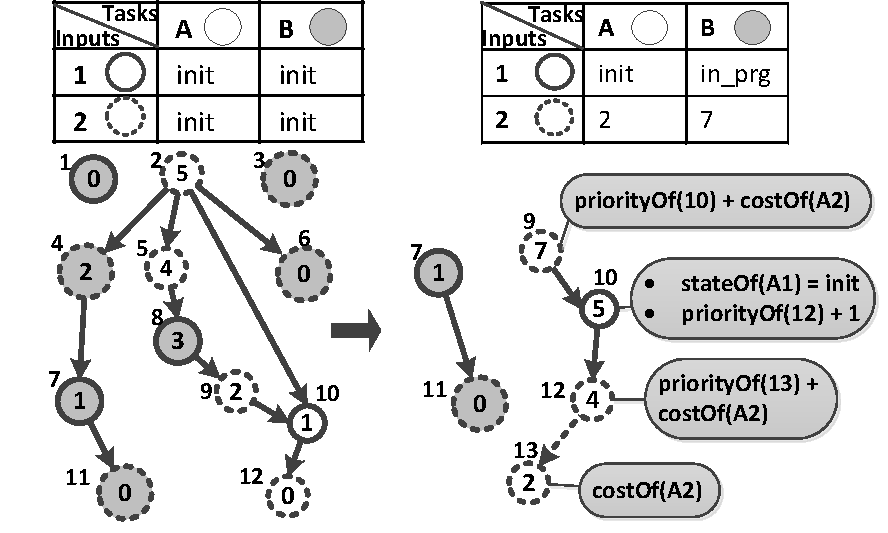
\includegraphics[width=\columnwidth]{images/hybrid_prioritization.pdf} 
\centering
\caption{Priority assignment with HYBRID scheduler. Priority update when the edge between tasks 12 and 13 is created}
\label{hybrid_priorities}
\vspace{-0.5cm}
\end{figure} 

Figure~\ref{hybrid_priorities} shows an example of task prioritization with HYBRID.
The tables show the state (or exec. time) of the tt-is pairs that appear on the TDG. Gray or white nodes indicate different task types (A or B respectively) and solid or dashed node outlines indicate task input size (1 or 2 respectively). The numbers inside the nodes show task priorities and the numbers outside the nodes show the task id.

On the leftmost TDG, the algorithm has no information about any of the tt-is costs.
As the leftmost table shows, for all the possible tt-is the state is \texttt{init} meaning no task has been executed yet.
Since the tasks of the TDG have been created, they have been prioritized using the CATS priority assignment method and the bottom level based priorities.
On the rightmost TDG, tasks 1, 2, 3, 4, 5, 6 and 8 have been executed and a new task has appeared on the TDG: task number 13.
When the edge 12$\rightarrow$13 is created, tasks begin to be prioritized.
Initially, the priority of the new task 13 is the cost of this task's tt-is, i.e., type A and input 2 (TaskA-Input2). 
Since there are no successors of this task, this becomes its initial priority.
Then, the \textit{plist} of task 13 is traversed and the priority of task 12 changes to priorityOf(13)+costOf(TaskA-Input2) since task 12 is corresponding to the TaskA-Input2 tt-is.
Moving to the upper levels, task 10 is of tt-is TaskA-Input1 that is on the \texttt{init} state, thus unknown cost.
This translates to the use of bottom level based prioritization so the priority of task 10 becomes priorityOf(12)+1.
Finally, task 9 is prioritized using the cost of the TaskA-Input2 tt-is and the TDG navigation stops since there are no other predecessors.

\if 0


Like CPATH, HYBRID prioritizes tasks according to their \textit{bottom cost} and/or their \textit{bottom level}.

HYBRID constitutes of three steps: \textit{Task Prioritization, Task Submission} and \textit{Task-to-core assignment.}


\subsubsection{Task prioritization}
The HYBRID scheduler prioritizes tasks according to their \textit{bottom cost} and/or their \textit{bottom level}.
The task prioritization step takes place during task creation.
%If when a dependency is created the execution time of the tt-is of the successor is known, then it is used for the prioritization.
If task cost information is available, HYBRID uses it to compute priorities.
Otherwise, the algorithm computes priorities the same way as CATS, that is, increasing the priority as we move to higher levels of the TDG.

%task execution time tracking:
As tasks are being executed HYBRID collects their execution times.
A vector is used to store the execution time of every tt-is discovered throughout the execution.
When a task finishes execution, HYBRID calls the \texttt{taskExit} function.
This function is responsible for tracking the execution time of the exiting task by storing it in the vector.
As in CPATH, \texttt{taskExit} ignores the first execution of every tt-is.
Therefore, the functionality of a small finite state machine is needed for each tt-is.
To start with, a tt-is is in the \texttt{init} state; when the tt-is has been executed once its state changes from \texttt{init} to \texttt{in$\_$progress} to skip the cost of the first execution.
After the second execution of the same tt-is, \texttt{taskExit} stores its execution time in the vector and its state becomes \texttt{tracked}.
This functionality is represented in the lines 2-9 of Listing~\ref{cpathExit}.
After this code, the function returns, since HYBRID does not perform any prioritization when a task is finishing execution.

The task prioritization step takes place when a new task is added to the TDG.
%Because the addition of a new task on the TDG always takes place at the (one) bottom of the graph, the use of the \textit{plist} (list of predecessors) of the tasks, is essential in order to perform a bottom-to-top TDG traversal.
HYBRID uses the \textit{plist} (list of predecessors as used in CATS) of the new task to navigate to the upper levels of the TDG and update the task priorities.

Listing~\ref{creation} shows the algorithm of the task prioritization with CATS.
Because HYBRID uses a very similar algorithm we will describe it using the same code while highlighting the differences.
When a new task is created, if its tt-is execution time is known, it is assigned as the priority of the new task. 
If there is no cost information the priority assigned to the new task is initially zero.
The \texttt{prioritize$\_$task} function is called on the creation of a new edge on the TDG between two tasks: the predecessor task and successor task.
It takes as argument the successor task and starts by traversing its \textit{plist} (line 5).
The HYBRID algorithm then checks whether the predecessor task has a tracked execution cost.
If so, it checks whether the priority of the current predecessor is lower than the priority of the successor plus the cost of the predecessor and, if this condition is met, the priority of the predecessor is updated accordingly.
In the case that the cost of the predecessor has not been tracked, the algorithm checks if the priority of the current predecessor is lower than the priority of the successor plus one (as on line 7 of Listing~\ref{creation}).
In the first case, HYBRID scheduler uses bottom cost based priorities, like CPATH, while in the latter case, it uses bottom level based priorities, like CATS.
In both cases, if the priority of the predecessor has changed and the predecessor task is a ready task (i.e. it sits on one of the ready queues) the corresponding ready queue is being reordered considering the updated priority (lines 9-10).

The same actions are performed for the predecessors of the upper levels of the TDG.
The algorithm, similarly to CATS, terminates if it encounters an empty \textit{plist} or if the priority of the current predecessor task (\texttt{currPred}) remains unchanged.


Figure~\ref{hybrid_priorities} shows an example of task prioritization with HYBRID.
The tables show the state (or the exec. time) of the tt-is pairs that appear on the TDG.
Gray or white nodes indicate different task types (type A or B respectively) and solid or dashed node outlines indicate the task input size (input 1 or 2 respectively).
The numbers inside the nodes show task priorities and the numbers outside the nodes show the task id.

On the left-most TDG the algorithm has no information about any of the tt-is costs.
As the left-most table shows, for all the possible tt-is the state is \texttt{init} meaning no task has been executed yet.
Since the tasks of the TDG have been created, they have been prioritized using the CATS priority assignment method and the bottom level based priorities.
On the right-most TDG tasks 1, 2, 3, 4, 5, 6 and 8 have been executed and a new task has appeared on the TDG: task number 13.
When the edge 12$\rightarrow$13 is created, tasks begin to get prioritized.
Initially, the priority of the new task 13 is the cost of this task's tt-is which is of type A and input 2 (A2). 
Since there are no successors of this task this becomes its initial priority.
Then, the \textit{plist} of task 13 is traversed and the priority of task 12 changes to the priorityOf(13)+costOf(A2) since task 12 is corresponding to the A2 tt-is.
Moving to the upper levels, task 10 is of tt-is A1 that is on the \texttt{init} state, thus unknown cost.
This translates to the use of bottom level based prioritization so the priority of task 10 becomes priorityOf(12)+1.
Finally, task 9 is prioritized using the cost of the A2 tt-is and the TDG navigation stops since there are no other predecessors.
\fi

\if 0
It then checks whether the priority of the current predecessor is greater than the priority of the successor





If the cost of a tt-is of a task is known at the time of the task's creation then this cost is used as priority to the task that is being created.
If the cost of the tt-is is unknown then the priority of the new task becomes \texttt{1}.

The result that we try to achieve in terms of priorities is the same as in Figure~\ref{cpath}. 
First, we need to track the task execution times.
HYBRID implements a simplified version of the function \texttt{taskExit} for doing so. 
The \texttt{taskExit} in HYBRID scheduler is responsible for tracking the execution time of each task-type/input size (tt-is) and store it to the time vector.
To simplify our description, the code of the HYBRID \texttt{taskExit} contains the lines 1-9 of Listing~\ref{cpathExit}.
While task costs are being tracked, other tasks are being prioritized.
The task prioritization step is similar to CATS shown in Listing~\ref{creation} featuring a minor difference. 
In the lines 7 and 8 of Listing~\ref{creation} HYBRID scheduler checks whether the cost of the current tt-is has been discovered; if it has been discovered, it increases the priority (\texttt{blev} in the code) by this cost, otherwise it increases the priority by 1.
This way, the tasks end up being prioritized with the bottom-cost-based priority as in the case of CPATH but only if the tt-is cost has been discovered.

%In this case this function simply checks if the execution time for the current task-type/input-size duple has been tracked.
%If not then we update the execution time of the timesSet with the elapsed time of the finished task.
%Meanwhile we use the \texttt{task$\_$prioritization} function; in this case, instead of always increasing the bottom-level by 1, the task$\_$prioritization querries the timesSet to find out whether the execution time has been computed.
%If we have a valid execution time, then the bottom level of the predecessor is increased by this value instead of 1.
\subsubsection{Task Submission and Task-to-Core Assignment}
The task submission and task-to-core assignment steps are identical to CPATH.


%For the task submission step we slightly modify the submit$\_$task function.
%In this case the scheduler has to keep track of the execution time of the last discovered critical task.
%By keeping this information available in the scheduler we can then decide if a successor belongs to the critical path by subtracting the maxExecution time instead of subtracting 1.
%Even if the execution time of the last discovered critical task is not known this returns a correct result because in case the execution time has not been tracked the lookup function returns 1 so automatically the bottom-level-based priority is taken into account.
%\subsubsection{Task-to-core assignment}
%This step is identical to the one of CATS.

The hybrid scheduler tries to compute the critical path in the most efficient way.
The critical path computation is approximate since the priorities on the TDG are not updated as soon as in the case of CPATH.
However even if the priorities do not take into account the execution time, the HYBRID manages to use the properties of CATS to perform well.
\kc{Maybe remove this sentence?:}
We expect that this scheduler will perform better if the input TDG features tasks that differ in execution time as well as if the TDG features a great number of tasks (e.g. thousands) so that their execution time is discovered before the end of their execution.

\fi

\subsection{Dynamic Heterogeneous Earliest Finish Time Scheduler}
The Heterogeneous Earliest Finish Time (HEFT) algorithm~\cite{HEFT} is a static scheduling approach for asymmetric systems.
HEFT consists of two compile-time phases that use profiling information: the \textit{task prioritizing phase} and the \textit{processor selection phase}.
In the first phase, the algorithm assigns priorities to the tasks based on their \textit{upward rank}, that is, the length of the critical path from a given task to the exit task including task computation and communication costs~\cite{HEFT}.
When task prioritizing is done, the tasks are sorted according to their priorities.
In the \textit{processor selection phase} the algorithm searches for each task the appropriate processor to execute it.
By keeping communication and computation costs, HEFT assigns each task to the processor that will finish its execution at the earliest possible time.
Topcuoglu et al. \cite{HEFT} present their results based on evaluation on synthetic TDGs and assume known task execution and communication times at compile time.
The scheduling is static, so all the decisions are taken before execution.

In this paper, since the evaluation consists of running real applications with unknown task costs, the best way to compare HEFT to our proposal is by using a dynamic version of HEFT algorithm (dHEFT).
The dHEFT is implemented in the OmpSs programming model and is based on the implementation used in the evaluation of CATS~\cite{Chronaki:ICS2015}.
This version assumes two different types of cores (fast and slow) and keeps records of the task costs in each core.
DHEFT discovers the task costs at runtime, computes the mean cost of each tt-is for each core type and then finds the core that will finish the task at the earliest possible time.

To find the earliest possible executor, dHEFT maintains
one list per core (wlist) including the ready tasks waiting
to be executed by that core. 
When a task becomes ready, dHEFT first inserts it in the ordered ready queue; then the task with the highest upward rank is selected and dHEFT checks if there are execution time records for this task. 
If the number of records is sufficient (we require a minimum of three records)
then the estimated cost of the task is considered stable. 
Using that estimated execution time, the task
is scheduled to the earliest executor by consulting the wlist
of all cores. If the number of records is not sufficient
for one of the core types, then the task is scheduled to the
earliest executor of this core type to get another record of
that task-type and core-type execution time. In all cases,
dHEFT updates the history of records on every task execution to adapt for phase changes in the application. \footnote{The time complexity of the task submission step is \textit{O($nN$)} and the task-to-core assignment is \textit{O($n$)}, where \textit{$n$} is the number of tasks and \textit{$N$} is the number of cores.}

The initial dHEFT version presented in previous work~\cite{Chronaki:ICS2015} lacks the \textit{task prioritizing phase} of the original HEFT algorithm.
This paper, uses an improved version of dHEFT that adds this functionality by prioritizing tasks according to their \textit{upward rank}.
The implementation of this is similar to the CPATH prioritization step.
%to the tasks whenever an undiscovered tt-is has finished its execution.
%The TDG is traversed from the top to the bottom and, using task execution times, the upward-rank-based priorities are assigned to tasks.
When the prioritized tasks become ready, they are inserted in a sorted ready queue in decreasing order of their priorities.
The algorithm then accesses the tasks in the order of their priorities to find the earliest executor for each of them.


%%%%%%%%%%%%%%%%%%%
%%%%%%%%%%%%%%%%%%%
%\section{Experimental Methodology}
%\label{sec:experimental}
%\begin{table*}[t]
\begin{center}
\caption{Evaluated benchmarks and relevant characteristics}
\label{tab.apps}
\resizebox{\textwidth}{!}{%
\begin{tabular}{|c|c|c|c|c|c|c|c|c|c|}
\hline
\multirow{3}{*}{\parbox{13mm}{\centering Application}} & 
\multirow{3}{*}{Problem size} & 
\multirow{3}{*}{\parbox{10mm}{\centering \#Tasks}} & 
\multirow{3}{*}{\parbox{17mm}{\centering Avg task CPU cycles (thousands)}} & 
\multicolumn{3}{|c|}{\parbox{22mm}{\centering Per task overheads (CPU cycles)}} & & &\\
\cline{5-7}
& & & & \multirow{2}{*}{\parbox{10mm}{\centering Create}} & \multirow{2}{*}{\parbox{9mm}{\centering All}} & \multirow{2}{*}{\parbox{11mm}{\centering Deps + Sched}} & \multirow{2}{*}{\parbox{15mm}{\centering Measured perf. ratio}} &
{\parbox{10mm}{\centering $r$}} &
\multirow{2}{*}{\parbox{11mm}{\centering Parallel model}} \\
& & & & & & & & & \\ %\hhline{~~~~~~}
\hline

\multirow{2}{*}{\parbox{18mm}{\centering Cholesky factorization}} & 
32K 256 & 357\,762  & 753 & 15221 &  73286 &  58065 &  \multirow{2}{*}{\parbox{9mm}{\centering 3.5}} & 10.34 & \multirow{2}{*}{\parbox{17mm}{\centering dependencies}}\\                                              & 32K 128 & 2829058 & 110 & 17992 &  58820 &  40828 & & 83.74 &\\
%& 32$\times$32 blocks of 512$\times$512 floats & 5984 & & 1\,551\,322 & 104.76 &  238.02 &  194.28  & \\ 
\hline{}
\multirow{2}{*}{\parbox{18mm}{\centering QR factorization}} & 16K 512 & 11\,442 & 518\,570  & 17595 & 63008 &   45413 & \multirow{2}{*}{\parbox{9mm}{\centering 6.8}} & 0.01 &\multirow{2}{*}{\parbox{17mm}{\centering dependencies}}\\
&  16K 128 & 707\,265 & 3\,558 & 21642 & 60777 & 39135 & & 3.11 &\\
\hline
Blackscholes & native & 488\,202 & 348  &   29141  &  85438 &  56297 & 2.3 & 42.87 & data-parallel \\
\hline
Bodytrack & native & 329\,123 & 383 &  9\,505 &  18979 & 9474 & 4.2 & 12.70 & pipeline \\ 
%Heat diffusion & Heat &  &  &  &  &  & \\ 
\hline
Canneal & native & 3\,072\,002 & 67 & 25781 & 50094 &  24313 & 2.0 & 197.01 & unstructured \\
\hline
Dedup & native & 20\,248 & 1\,532 & 1294 & 9647 &  8353 & 2.7 & 0.43 & pipeline \\
\hline 
Ferret & native$\times$2 & 84\,002 & 29\,088 & 38913 & 98457 &  59544 & 3.6 & 0.68 & pipeline \\
\hline
Fluidanimate & native & 128\,502 & 16\,734 & 30210 & 94079 &  64079 & 3.3 & 0.91 & data-parallel \\
\hline
Streamcluster & native & 3\,184\,654 & 161 & 6892 & 13693 &  6801 & 3.5 & 21.91 & data-parallel \\
\hline
\end{tabular}}
\end{center}
\vspace{-0.4cm}
\end{table*}

\subsection{Applications}
%\begin{itemize}
%\item Blackscholes
%\item Cholesky
%\item Canneal
%\item Fluidanimate
%\item QR Factorization
%\item Bodytrack
%\item Streamcluster
%\end{itemize}
Table~\ref{tab.apps} shows the evaluated applications, the input sizes used, and their characteristics. 
All applications are implemented using the OpenMP programming model~\cite{OpenMP4.0:Manual2015}. 
We obtain Cholesky and QR from the BAR repository~\cite{BAR} and we use the implementations of the rest of the benchmarks from the PARSECSs suite~\cite{Chasapis:TACO2016}.
More information about these applications can be found in~\cite{Chasapis:TACO2016} and~\cite{Chronaki:ICS2015}.
As the number of cores in SoCs is increasing, so does the need of available task parallelism~\cite{Sanchez:2010}. 
We choose the input sizes of the applications so that they create enough fine-grained tasks to feed up to 512 cores.
The number of tasks per application and input as well as the average per-task CPU cycles can be found on Table~\ref{tab.apps}.





\subsection{Simulation}
\label{TaskGenX:experimental:simulation}
To evaluate TaskGenX we make use of the TaskSim trace-driven simulator~\cite{AbstrLevels_TACO12,MUSA} as explained in Section~\ref{sec.background.simulation}. 

We evaluate both symmetric and asymmetric systes with the number of cores varying from 8 to 512.
To set the correct performance ratio between big and little cores for the asymetric systems, we measure the sequential execution time of each application on a real ARM big.LITTLE platform when running on a little and on a big core. 
We use the Hardkernel Odroid~XU3 board that includes a Samsung Exynos 5422 chip with ARM big.LITTLE.
The big cores run at 1.6GHz and the little cores at 800MHz.
Table~\ref{tab.apps} shows the measured performance ratio for each case.
The average performance ratio among our 11 workloads is 3.8.
Thus in the specification of the asymmetric systems we use as performance ratio the value 4.

We modify TaskSim so that it features one extra hardware accelerator (per multi-core) responsible for the fast task creation (the RTopt).
Apart from the task duration time, our modified simulator tracks the duration of the runtime overheads.
These overheads include: (a) task creation, (b) dependencies resolution, and (c) scheduling.
The RTopt core is optimized to execute task creation faster than the general purpose cores; 
to determine how much faster a task creation job is executed we use the analysis performed in Section~\ref{sec:hw_req}.

Using Equation~\ref{eq.create}, we compute the $C_{opt}(x)$ for each application according to their average task CPU cycles from Table~\ref{tab.apps} for $x=512$ cores.
$C_{gp}$ is the cost of task creation when it is performed on a general purpose core, namely the \textit{Create} column shown on Table~\ref{tab.apps}.
To have optimal results for each application on systems up to 512 cores, $C_{gp}$ needs to be reduced to $C_{opt}(512)$.
Thus the specialized hardware accelerator needs to perform task creation with a ratio $r = C_{gp}/C_{opt}(512) \times$ faster than a general purpose core.

We compute $r$ for each application shown on Table~\ref{tab.apps}. We observe that for the applications with a large number of per-task CPU cycles and relatively small \textit{Create} cycles (QR512, Dedup, Ferret, Fluidanimate), $r$ is very close to zero, meaning that the task creation cost ($C_{gp}$) is already small enough for optimal task creation without the need of a faster hardware accelerator.
For the rest of the applications, more powerful hardware is needed.
For these applications $r$ ranges from 3$\times$ to 197$\times$.
Comparing $r$ to the measured performance ratio of each application we can see that in most cases accelerating the task creation on a big core would not be sufficient for achieving higher task creation rate.
In our experimental evaluation we accelerate task creation in the RTopt and we use the ratio of 16$\times$ which is a relatively small value within this range that we consider realistic to implement in hardware.
%Contrarily, if RTopt is assigned a task to execute, we assume that it executes it 4$\times$ slower than a general purpose in-order core.
The results obtained show the average results among three different traces for each application-input.

%%%%%%%%%%%%%%%%%%%
%%%%%%%%%%%%%%%%%%%
\section{Evaluation}
\label{sec:evaluation}
\section{Evaluation}
\label{sec.scheduling.evaluation}


\subsection{Methodology}
\begin{figure}[t]
	\centering
	\subfloat[Cholesky 8$\times$8]{
		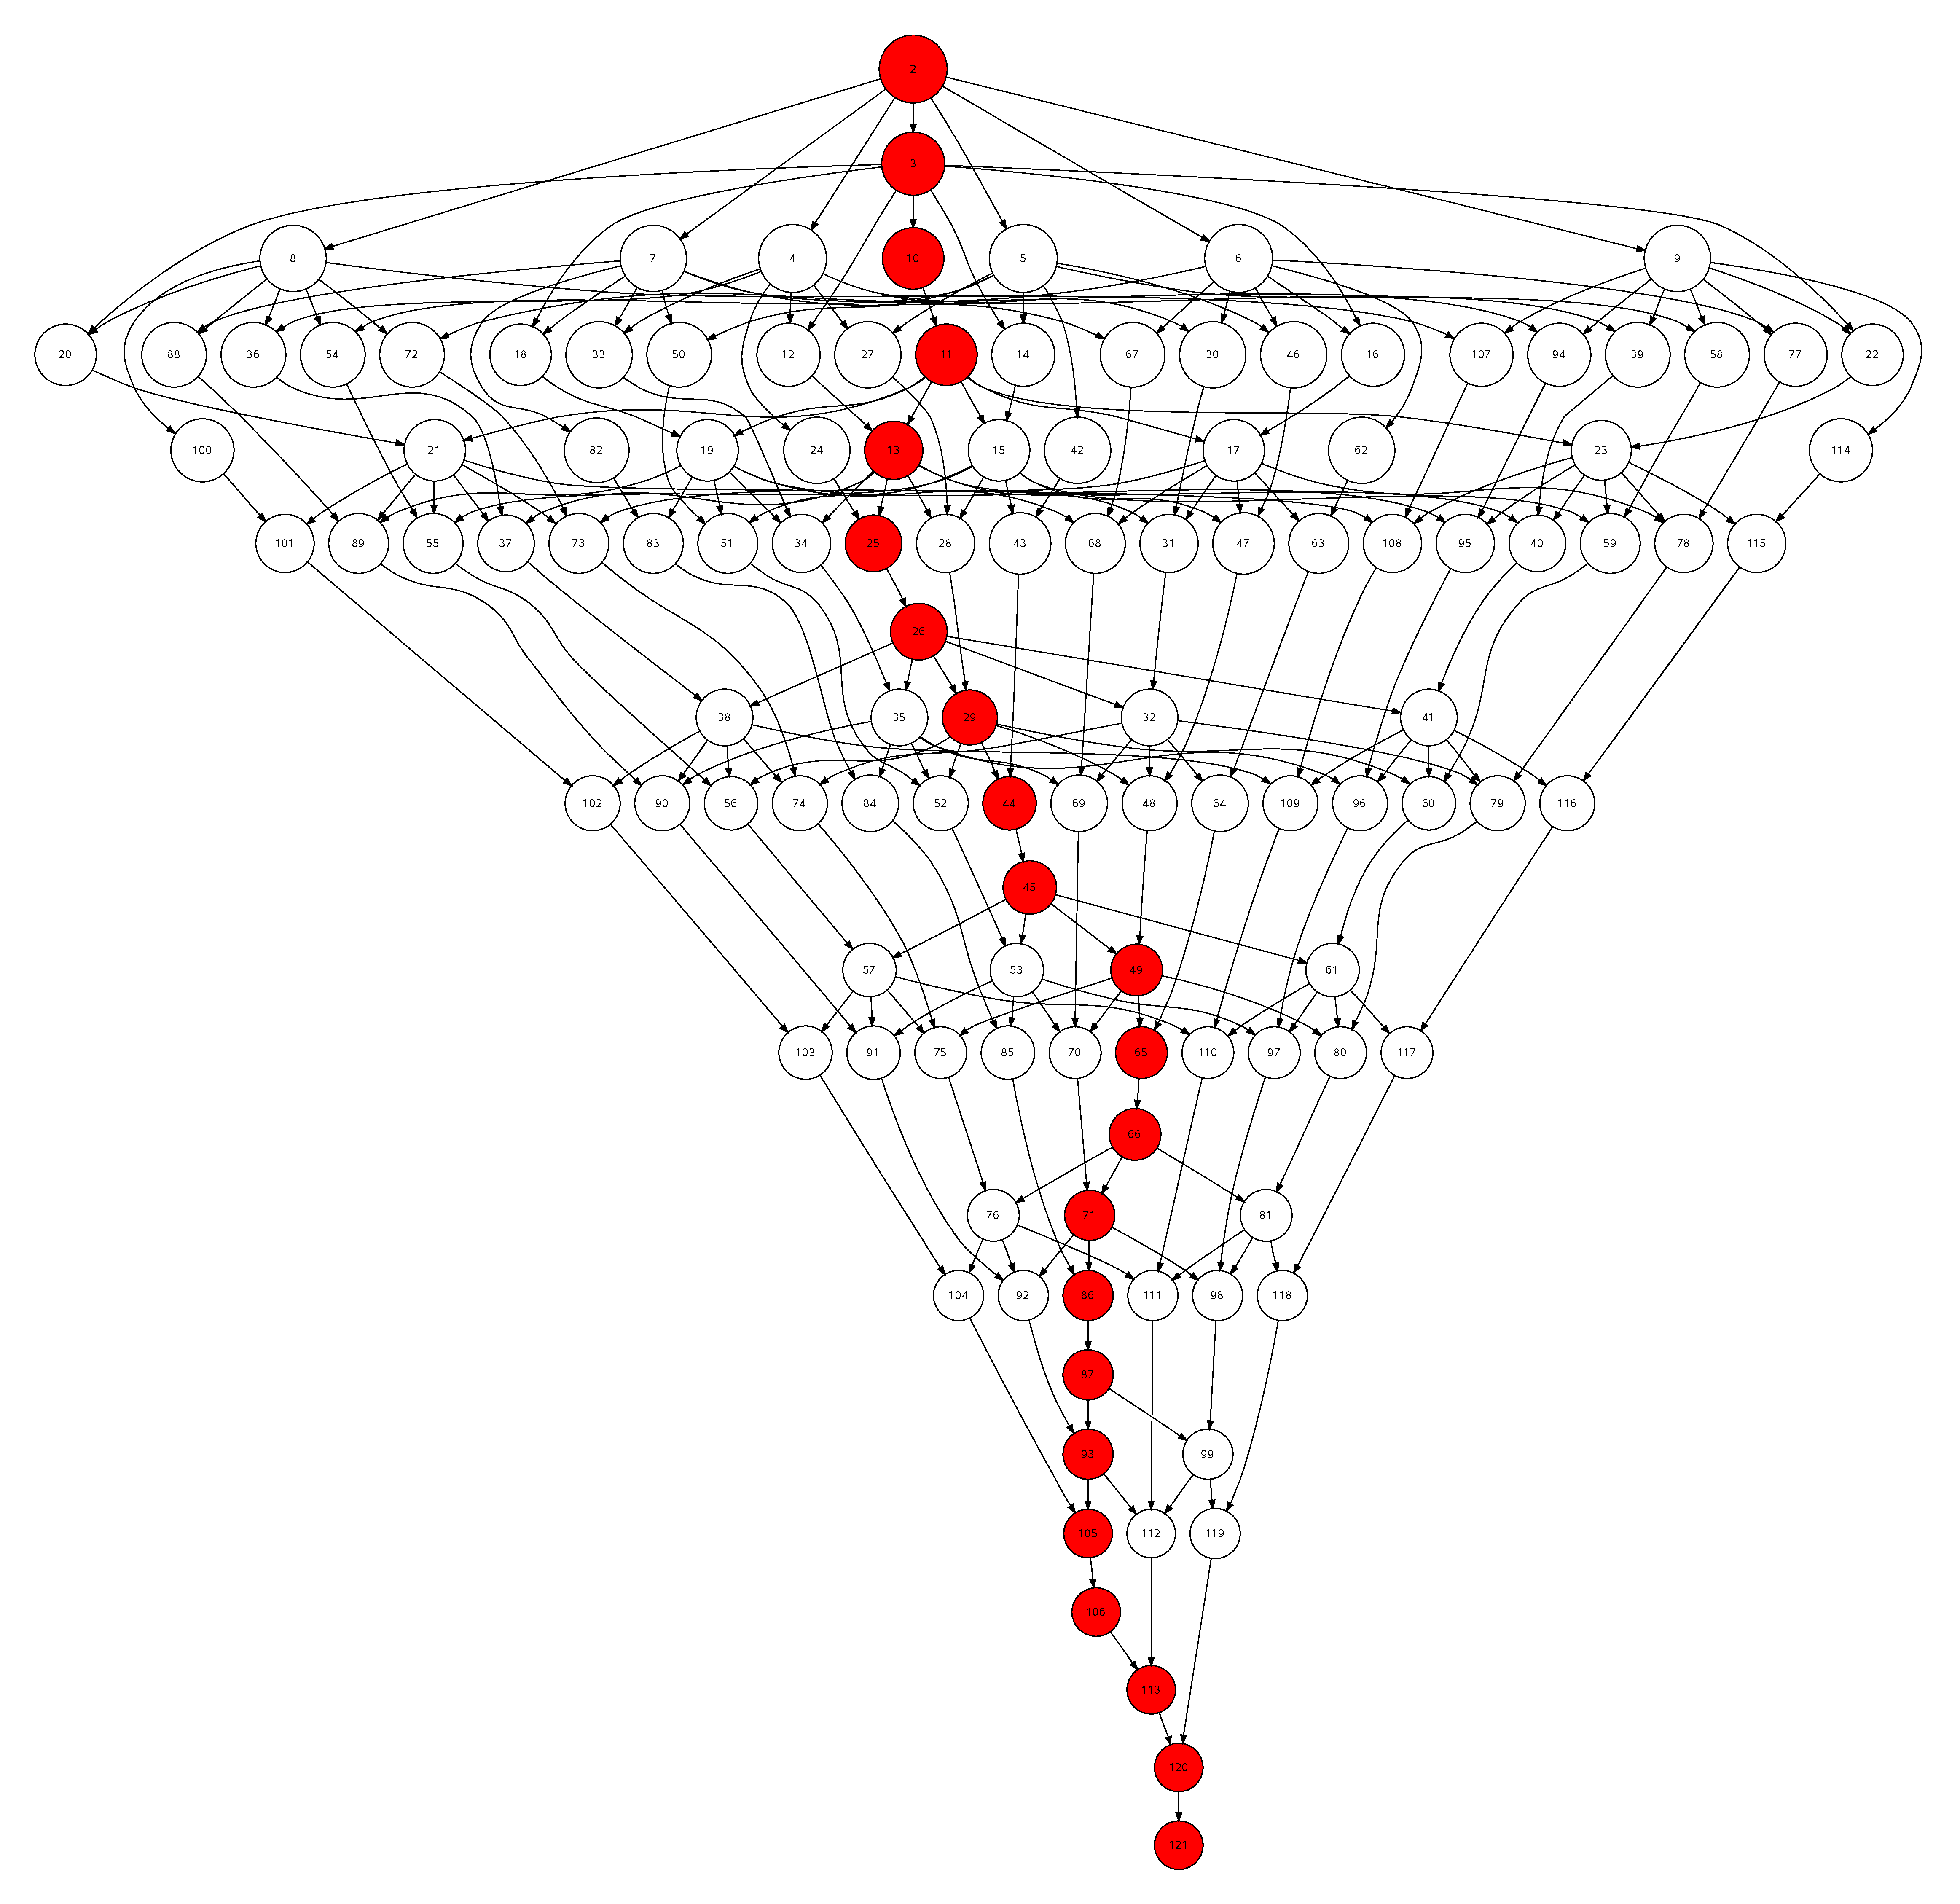
\includegraphics[width=0.26\textwidth]{images/cholesky_8_white.pdf}
		\label{cholesky8x8_TDG}
	}
	\subfloat[Cholesky 16$\times$16]{
		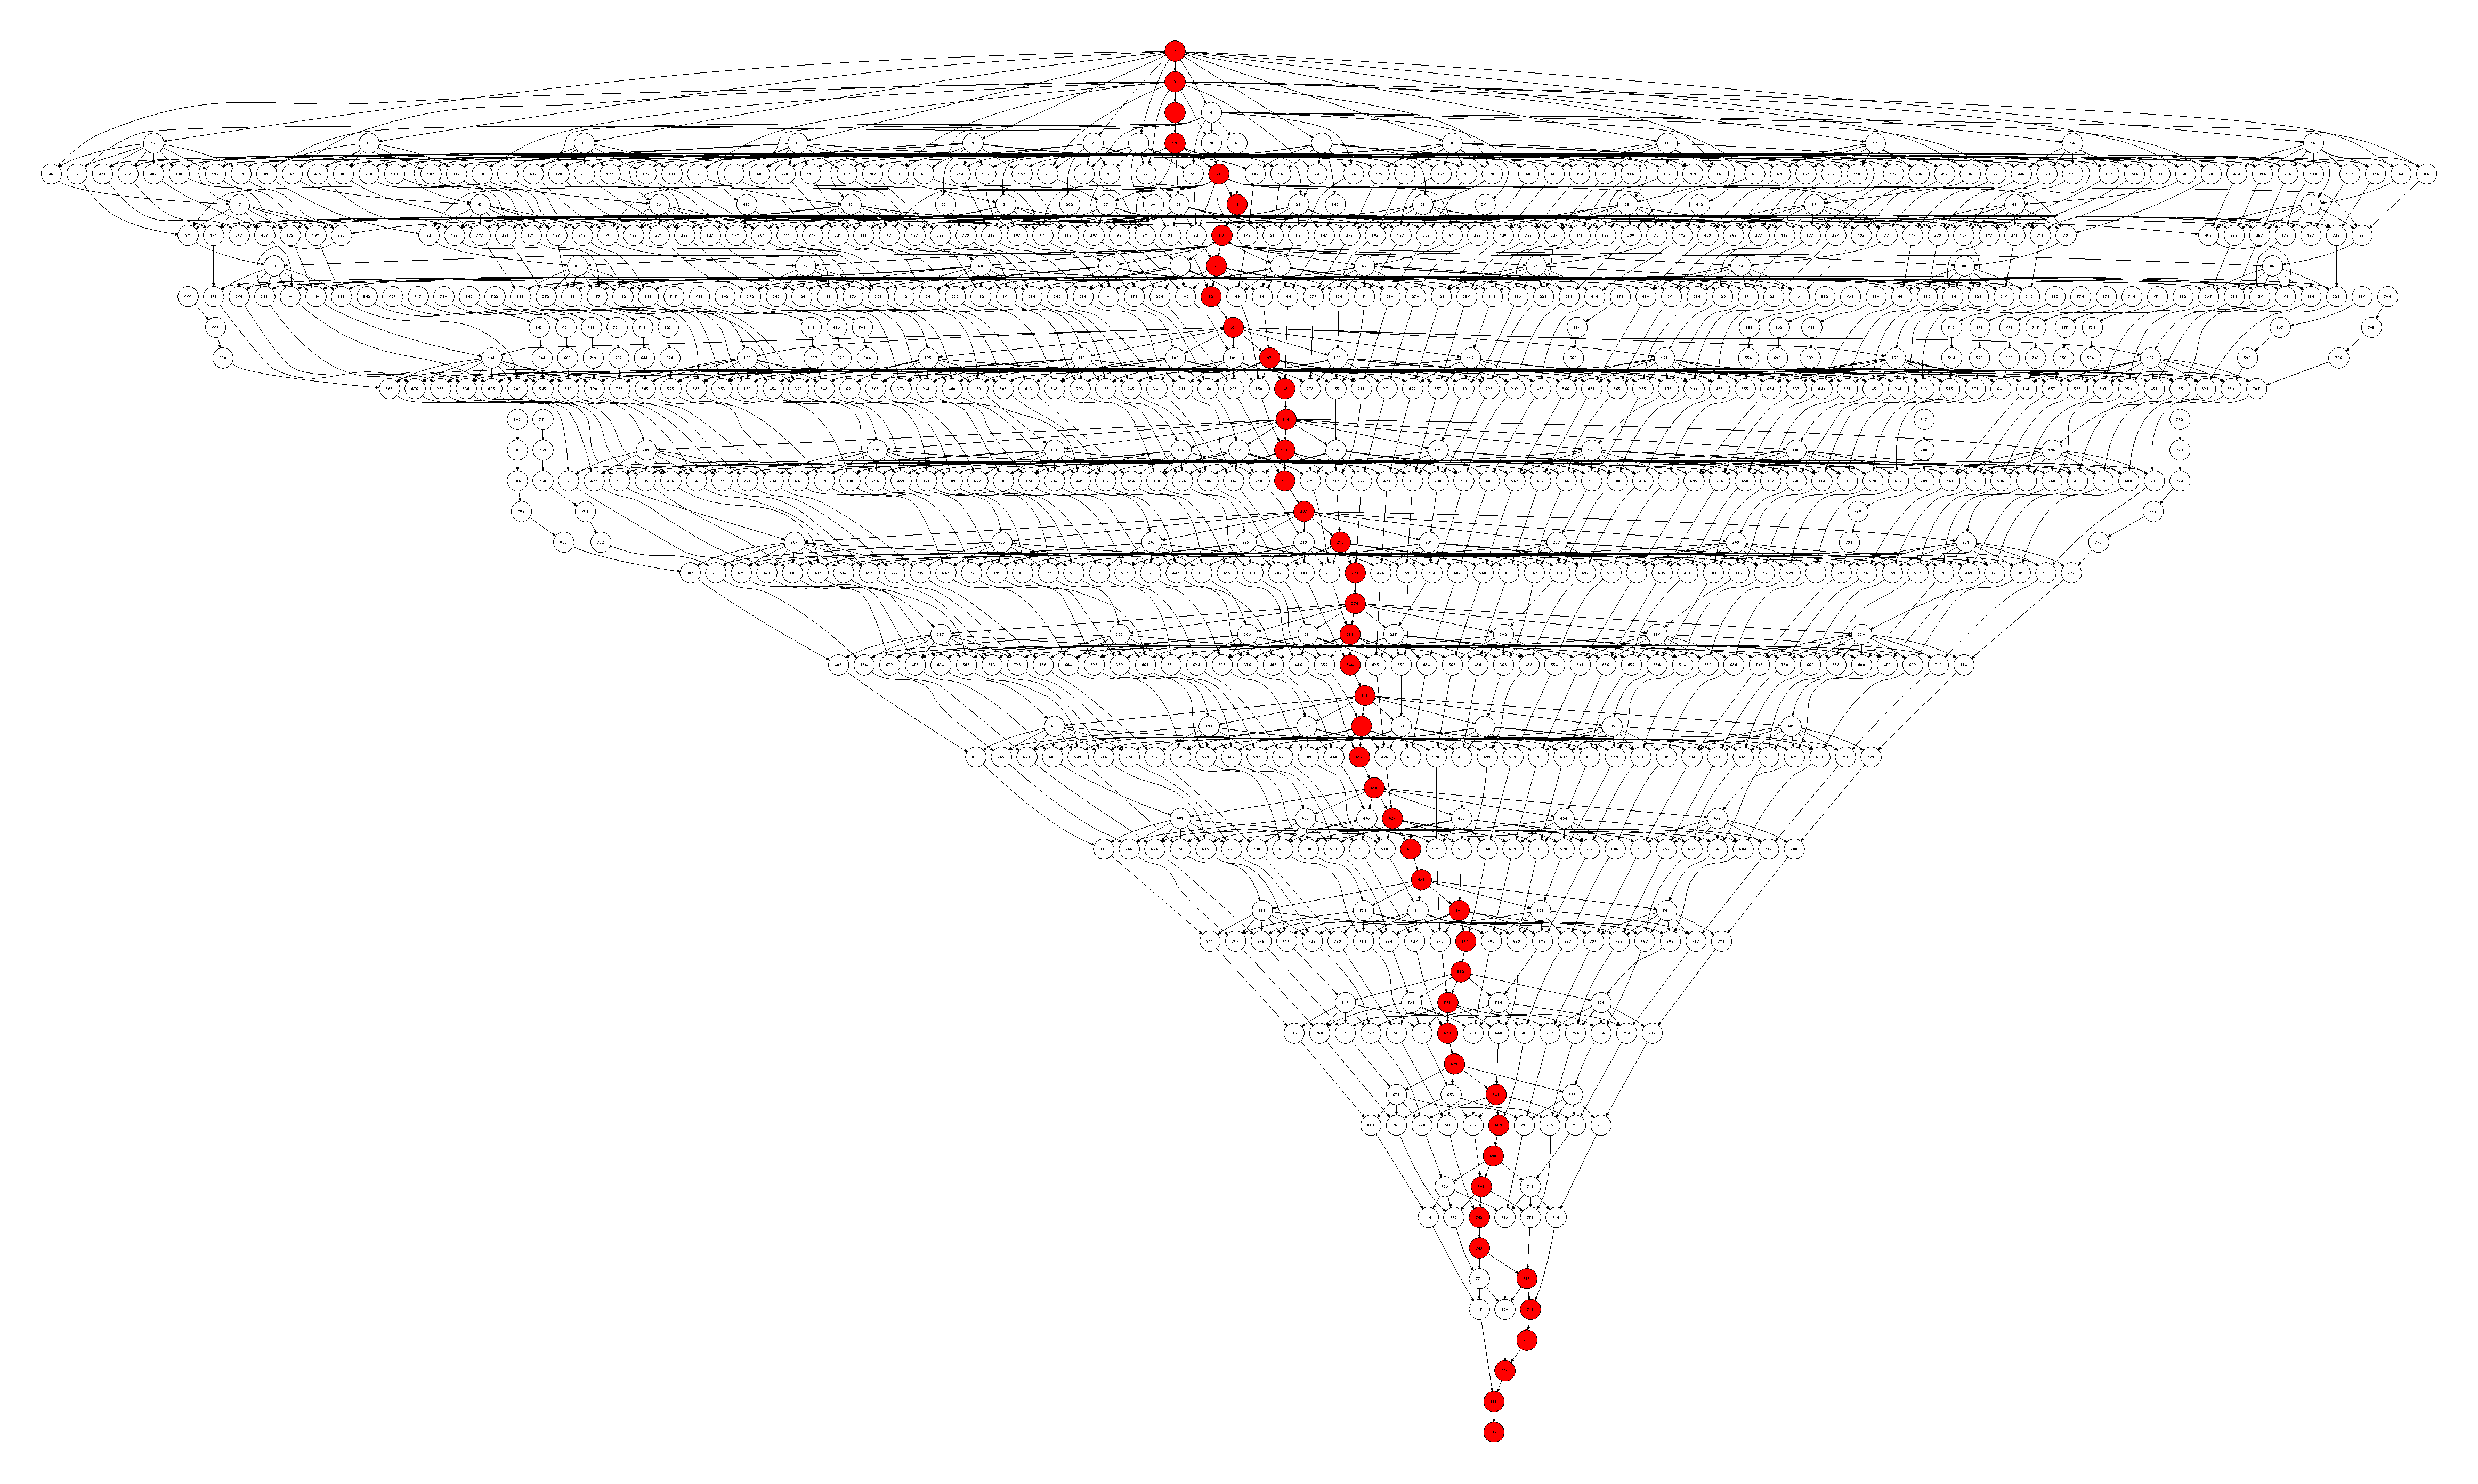
\includegraphics[width=0.6\textwidth]{images/cholesky_16_white.pdf}	
		\label{cholesky16x16_TDG}
	}
	\caption{Cholesky factorization task dependency graphs.}
	\label{fig.cholesky_graphs}
\end{figure}
% For example, a multi-core chip with some in-order cores and some out-of-order cores. The evaluation part of this paper contains real machine evaluation as well as evaluation through simulation.

%CATS targets heterogeneous multi-core systems with cores that expose different characteristics in terms of performance and power. We perform experiments on ODROID XU3 8-core platform. The ODROID XU3, features the ARM big.LITTLE technology offering heterogeneous multi-processing. Moreover, we simulate the behaviour of our design to estimate the impact of CATS on heterogeneous systems with a larger amount of cores and different performance ratios.
%On the simulated platform we are able to set up different performance ratios between fast and slow cores without a restriction.

In the first part of our real environment evaluation, we measure the execution time of four criticality-sensitive applications using CATS ad the default OmpSs scheduler. 
We evaluate four different CATS configurations based on the options explained in Section~\ref{sec.scheduling.cats} and provide a detailed comparison between them. 
The options consist of whether the task submission policy is strict or flexible, and the type of the work stealing mechanism. 
This results in the following configurations:
\begin{itemize}
	\itemsep0em
	\item Flexible with simple work stealing (SS FLEX)
	\item Flexible with bidirectional work stealing (2DS FLEX)
	\item Strict with simple work stealing (SS STRICT)
	\item Strict with bidirectional work stealing (2DS STRICT)
\end{itemize}

\kc{should it stay or should it go???:}
The default OmpSs scheduler employs a \textit{breadth-first} policy~(BF)~\cite{Duran_schedulers_08}. The BF scheduler implements a single first-in-first-out ready queue shared among all threads. 
When a task is ready, it is inserted in the tail of the ready queue and when a core becomes available, it retrieves a task from the head of the queue. Tasks are ordered according to their ready time: the earliest ready task resides at the head of the queue. Since the ready queue is shared, there is no need for work stealing and the load is balanced automatically. BF does not differentiate among core types and assigns tasks in a first-come-first-served basis.

After the analysis of the CATS configurations we measure the execution time of five applications using CATS, CPATH, HYBRID, dHEFT and the default OmpSs BF scheduler that is explained in Section~\ref{sec.background.taskbased.ompss}. 
The execution time corresponds to the average of 10 executions of the application on each machine set-up.

%%%%%%%%%%%%%%%%%%%%%%%%%%%%%%%%%%%
\if 0 % about strict/flexible
As it is already shown in previous works~\cite{Chronaki:ICS2015}, the most efficient CATS configuration is when using the simple work stealing and flexible policy (SSFLEX).
The same applies for CPATH and HYBRID schedulers, thus the results presented in this section refer to this configuration of the schedulers. 
\fi %%%%%%%%%%%%%%%%%%%%%%%%%%%%%%%%
Our test bed comprises a real big.LITTLE processor and a simulated heterogeneous system.

%The default OmpSs scheduler employs a \textit{breadth-first} policy~(BF)~\cite{Duran_schedulers_08}. The BF scheduler implements a single first-in-first-out ready queue shared among all threads. When a task is ready, it is inserted in the tail of the ready queue and when a core becomes available, it retrieves a task from the head of the queue. Tasks are ordered according to their ready time: the earliest ready task resides at the head of the queue. Since the ready queue is shared, there is no need for work stealing and the load is balanced automatically. BF does not differentiate among core types and assigns tasks in a first-come-first-served basis. We use this scheduler as a baseline for the evaluation.

%%TODO this needs to be rephrased and more structured...
%We implement a dynamic version of HEFT scheduler (dHEFT) in the OmpSs programming model. The implementation assumes two different types of cores (big and little) and keeps records of the tasks' execution times in each core. The original HEFT \cite{HEFT} implementation assumes the prior knowledge of the TDG as well as the costs of the tasks. In our case, since the evaluation consists of running benchmarks, best way to compare HEFT and the other approaches is to keep the scheduling idea of HEFT and transform it from a static scheduler to a dynamic scheduler. This means that during runtime dHEFT discovers the costs of the tasks, computes a mean value of the costs for each task-type, parameter-size duple for each type of processor and then finds the processor that will finish the task at the earliest possible time. A difference between the static HEFT and dHEFT is the order that the tasks are being submitted. In HEFT tasks are submitted in decreasing order of their upward rank, which is computed statically with the known task costs. Since dHEFT discovers the costs while tasks are executing, there is no priority in the task submission. In dHEFT tasks are submitted as soon as they become ready. To find the earliest possible executor, dHEFT maintains one list per core (\textit{wlist}) with the ready tasks that are waiting to be executed by this core. When a task is submitted, dHEFT first checks if there are records of prior execution of this task. If the number of records is sufficient (in our experiments we use 3 records at least) then the estimated execution time of the task is considered stable. So, the task is scheduled to the earliest executor by consulting the \textit{wlist} of all the processors. If the number of records is not sufficient for one of the processor types then the task is scheduled to the earliest executor of this processor type. In any case dHEFT creates history by storing every time the task cost in the appropriate records in order to maintain stable results in the next submissions.

To perform our experiments, we use the Hardkernel \textbf{Odroid-XU3} development board that has an 8-core Samsung Exynos 5422 with an ARM big.LITTLE architecture. 
This platform is described in detail in section~\ref{sec.background.arm}.
%The Hardkernel \textbf{Odroid-XU3} development board has an 8-core Samsung Exynos 5422 chip with an ARM big.LITTLE architecture and 2GB of LPDDR3 RAM at 933MHz. The chip has four Cortex-A15 cores clocked at 1.6GHz and four Cortex-A7 cores at 800MHz. The four Cortex-A15 cores form a \textit{cluster} with a shared 2MB L2 cache, and the Cortex-A7 share a 512KB L2 cache. The two \textit{clusters} are coherent, so a single shared memory application can run on both clusters, using up to eight cores simultaneously. 
In our experiments, we evaluate a set of possible combinations of fast and slow cores varying the total number of cores from two to eight. 
%For the remainder of this section, we refer to Cortex-A15 cores as \textit{big} and to Cortex-A7 cores as \textit{little}.

% Talking about the performance ratio of the applications before describing the applications sound a bit strange, let's move this to applications section
%Depending on the workload, big and little cores expose different performance ratios. For example, a double precision benchmark advances a big core to be 3$\times$ faster than a little core, while for integer operations a big core is 1.9$\times$ faster than a little one \cite{Greenhalgh2011}. To get the notion of this performance ratio, we perform an execution of each application in one big core and another identical execution in one little core. The difference in performance on these two execution defines the difference in performance for big and little cores for each specific workload. Table \ref{tab.apps} shows the performance ratios explored for the benchmarks that we use.

%According to the calculated performance ratio, we can export the upper bound on speedup over a little core for each benchmark when running on 8 cores. Equation \ref{eq.ideal} shows how the ideal speedup is computed and assumes that the workload can be fully parallelized with zero dependencies, overheads or sequential sections in the application, according to Amdahl's law \cite{Amdahl}.
%\begingroup\makeatletter\def\f@size{9}\check@mathfonts
%\begin{equation}
%  \text{IDspeedup(workload, 8) = 4 $\times$ perf\_ratio(workload) + 4}
%\label{eq.ideal}
%\end{equation}
%\endgroup


%% Replaced for anonimity
%\subsubsection{TaskSim}

%Heterogeneous platforms such as ODROID-XU3 are currently limited in terms of size. We expect that future heterogeneous platforms will grow bigger with a larger amount of cores and various performance differences between fast and slow cores. 
To evaluate heterogeneous scheduling on larger multi-core systems we use the heterogeneous multi-core TaskSim simulator~\cite{AbstrLevels_TACO12} described in section~\ref{sec.background.simulation}. TaskSim allows the specification of a heterogeneous system with two different types of cores: fast and slow. 
We can configure the amount of cores of each type and the difference in performance between the different types (performance ratio) in the TaskSim configuration file.
In our experiments, we evaluate the effectiveness of the schedulers on 8 distinct heterogeneous machine configurations. 
These comprise systems with 16 or 32 total number of cores, and the number of fast cores ranging from 1 to 16. 
We set the performance ratio between fast and slow cores to 4.5$\times$ because this is the average performance ratio observed on the real machine for the benchmarks of this evaluation.

%For all these configurations, we evaluate the following performance ratios between fast and slow cores: 2$\times$, 2.5$\times$, 3$\times$, 3.5$\times$ and 4$\times$.

%% moved here because we needed to know about the heterogeneous platforms before talking about big and little cores

%The metric used in the following charts for each pair (\textit{total number of cores, number of big cores}), is the improvement of CATS over the baseline scheduler as well as the speedup obtained for each policy over one LITTLE core. The improvement is computed as shown in Equation~\ref{eq.improvement} and the speedup is computed as shown in Equation~\ref{eq.speedup}.

%% This, we are already saying in the explanation of the platforms
%

For both real and simulated platforms, each set-up has a given number of \textit{total} and \textit{big} cores.
%Our metrics are the improvement of CATS over the baseline scheduler, and the 
For all the scheduling approaches we present their speedup over the execution on one \textit{little} core, shown in Equation~\ref{eq.sched.speedup}. 
%Equations~\ref{eq.improvement} and~\ref{eq.speedup} show the improvement and speedup calculations.
%Equation~\ref{eq.speedup} shows how speedup is calculated in this evaluation.
\begingroup\makeatletter\def\f@size{8}\check@mathfonts
%\begin{equation}
%  \text{Improv. over BF(total, big)} = \frac{\text{Exec. time BF(total, big)}}%{\text{Exec. time CATS(total, big)}}
%\label{eq.improvement}
%\end{equation}
\begin{equation}
  \text{Speedup(total, big)} = \frac{\text{Exec. time(1, 0)}}{\text{Exec. time(total, big)}}
  \label{eq.sched.speedup}
\end{equation}
\endgroup


\subsubsection{Applications}

\begin{table*}
	\scriptsize
	\begin{center}
		\caption{Evaluated benchmarks and relevant characteristics. The inputs of QR and Heat diffusion are arrays of doubles and the inputs of Cholesky and Int. Histogram are arrays of floats.}
		\label{tab.sched.apps}
		\begin{tabular}{|c|c|c|c|c|c|c|c|c|}
			\hline
			\multirow{2}{*}{\parbox{10mm}{\centering Application}} & 
			\multirow{2}{*}{\parbox{9mm}{\centering Problem size}} & 
			\multirow{2}{*}{\parbox{9mm}{\centering \#Tasks}} & 
			\multirow{2}{*}{\parbox{9mm}{\centering \#Task types}} & 
			\multirow{2}{*}{\parbox{18mm}{\centering Avg task exec. time (${\mu}s$)}} & 
			\multicolumn{3}{|c|}{Per task overheads (${\mu}s$)} &\\
			\cline{6-8}
			& & & & & {\parbox{10mm}{\centering CATS}} & {\parbox{10mm}{\centering CPATH}} & {\parbox{11mm}{\centering HYBRID}} &
			
			\multirow{2}{*}{\parbox{13mm}{\centering Measured perf. ratio}} \\
			& & & & & & & & \\ %\hhline{~~~~~~}
			\hline
			
			\multirow{3}{*}{Cholesky} 
			& 8K 1024 & 120 & & 10\,314\,660 & 81.19 &  115.29 &  112.41 & \\                                              
			& 8K 512 & 816 & 4 & 1\,551\,322 & 104.76 &  238.02 &  194.28 &3.48 \\ 
			& 16K 512 & 5984 & & 1\,551\,322 & 104.76 &  238.02 &  194.28  & \\ 
			\hline{}
			QR & 8K 512 & 1\,496 & 4 & 11\,651\,079  &   1\,419.33 & 2\,580.41 &   1\,451.74 & 6.86 \\ 
			\hline
			Heat diffusion & 8K 512 & 5\,124 & 3 & 93\,198  &   145.17  &  748.84 &  170.00& 3.68 \\
			\hline
			Int. Histogram & 8K 512 & 2\,048 & 2 & 514\,096 &  217.45 &  62.07 & 263.62  & 2.23 \\ 
			%Heat diffusion & Heat &  &  &  &  &  & \\ 
			\hline
			Bodytrack & native & 408\,525 &  6 & 41\,869 & 93.90 & 120.93 &  120.93 & 4.14 \\
			\hline
		\end{tabular} 
	\end{center}
\end{table*}
\normalsize
\begin{figure}[t]
	\centering
	\subfloat[Cholesky 8$\times$8]{
		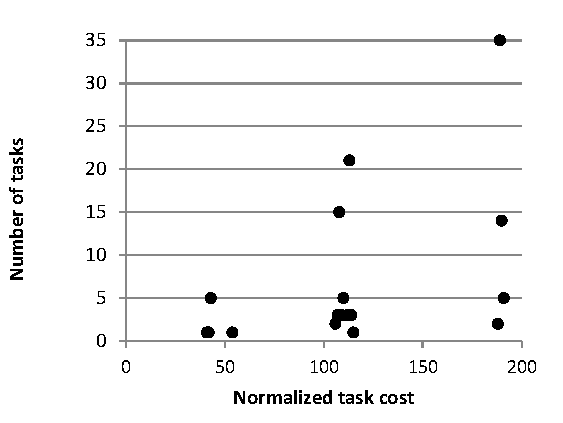
\includegraphics[width=0.3\textwidth]{images/cholesky_8x8_distribution.pdf}
		\label{cholesky8x8_dist}
	}
	\subfloat[Cholesky 16$\times$16]{
		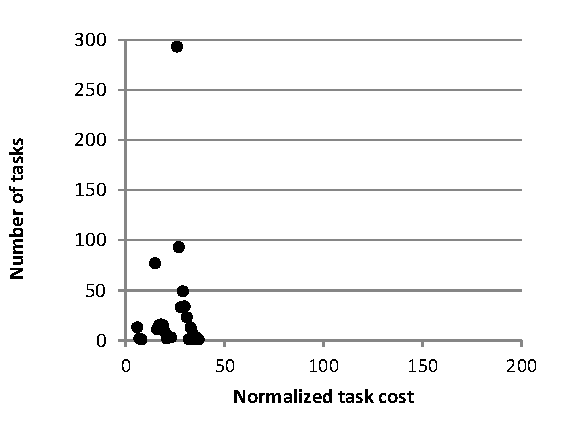
\includegraphics[width=0.3\textwidth]{images/cholesky_16x16_distribution.pdf}	
		\label{cholesky16x16_dist}
	}
	\subfloat[QR factorization]{
		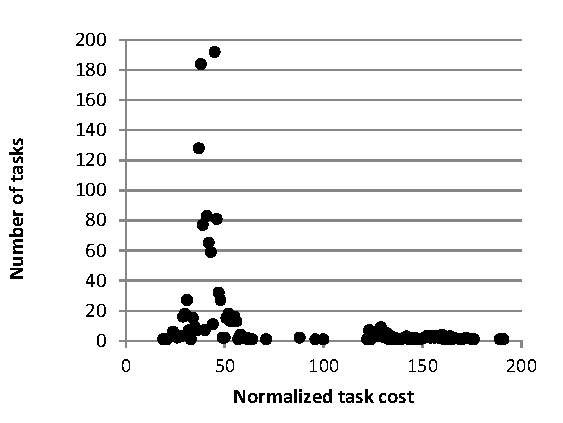
\includegraphics[width=0.3\textwidth]{images/QR_16x16_distribution.pdf}	
		\label{qr_dist}
	}
	\\
	\subfloat[Heat diffusion]{
		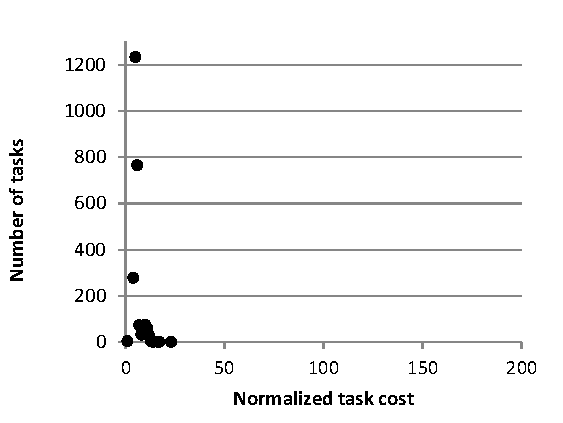
\includegraphics[width=0.3\textwidth]{images/heat_16x16_distribution.pdf}	
		\label{heat_dist}
	}
	\subfloat[Integral Histogram]{
		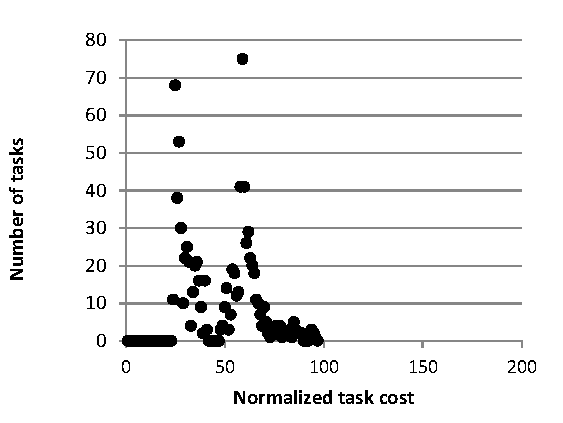
\includegraphics[width=0.3\textwidth]{images/histogram_8x8_distribution.pdf}	
		\label{histogram_dist}
	}
	\subfloat[Bodytrack]{
		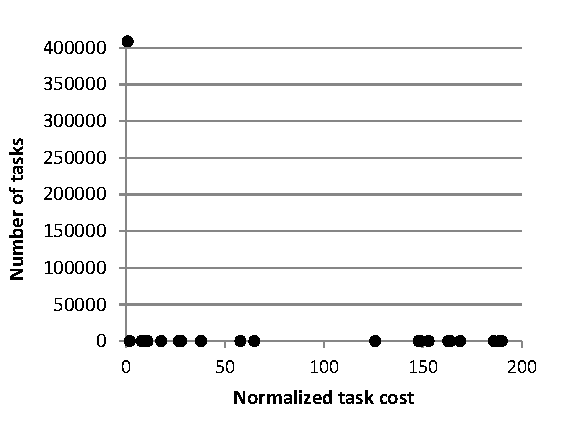
\includegraphics[width=0.3\textwidth]{images/bodytrack_native_distribution.pdf}	
		\label{bodytrack_dist}
	}
    \caption{Task cost distribution for each application. Results are based on 4BIG-core executions. $x$ axis shows the cost of the tasks and $y$ axis shows the number of tasks with the corresponding task cost.}
  \label{distributions}
  %\vspace{-0.4cm}
\end{figure}

We use five scientific applications implemented in the OmpSs programming model: Cholesky factorization, QR factorization, Heat diffusion, Integral Histogram and Bodytrack, also described in Section~\ref{sec.background}. 
These benchmarks are accessible in the BSC Application Repository~\cite{BAR} and in the PARSECSs library~\cite{Chasapis:TACO2016}. 


%\subsubsection{Bodytrack}
%\textbf{Bodytrack} is an application that tracks a marker-less human body using multiple cameras through an image sequence. 
%The OmpSs version implements a two-stage parallel pipeline for the image processing.
%%In the first stage the implementation allows the concurrent processing of all the frames of the image sequence. 
%%The second stage is the application of a particle filter to the images in order to mark the human body.
%The two stages are synchronized through the OmpSs dataflow annotations.
%By allowing the parallel processing of frames, OmpSs achieves the overlapping of the I/O and serial code with the tasks. 
%We use the native input of the benchmark suite~\cite{Chasapis:TACO2016}.

%Their different configurations and characteristics are shown in Table~\ref{tab.apps}.
%
%The applications have different sensitiveness depending on the inter-task dependencies that determine the available parallelism and the percentage of critical tasks, shown in the table. The larger proportion of critical tasks, the larger the potential improvement of CATS, as these are tasks that, once accelerated, reduce the application overall execution time. The percentage of critical tasks in Table~\ref{tab.apps} is from a single-core execution of CATS. Since CATS is dynamic, the tasks considered critical would be different for different configurations, since the algorithm runs on a partial dependency graph, including only the outstanding tasks. However, the single-core figures serve as an estimation of the percentage of critical tasks intrinsic to the overall application, that allows us to reason about the results with respect to this application characteristic.
%
%The percentage of critical tasks characterises the shape of the task dependency graph. The larger the proportion of critical tasks, the narrower the graph. These percentages, are exported from a single-core CATS execution of each kernel. So, this shows the theoretical amount of critical tasks that CATS discovers, since a multi-core execution of the application would detect the longest path dynamically. Nevertheless, it is shown experimentally that an application with a higher theoretical percentage of critical tasks has a higher number of critical tasks in practice, than an application with a small theoretical percentage of critical tasks.
%
%Depending on the workload, big and little cores expose different performance ratios. For example, a double precision benchmark advances a big core to be 3$\times$ faster than a little core, while for integer operations a big core is 1.9$\times$ faster than a little one \cite{Greenhalgh2011}. To get the notion of this performance ratio, we perform an execution of each application in one big core and another identical execution in one little core. The difference in performance on these two execution defines the difference in performance for big and little cores for each specific workload. Table \ref{tab.apps} shows the performance ratios explored for the benchmarks that we use.
%IDEAL SPEEDUP
%The performance ratios in Table~\ref{tab.apps} are computed for the real machine by comparing the execution time on one little core over the execution time on one big core. Using these performance ratios, we can estimate the ideal speedup over a little core for each application running on all eight cores. Equation~\ref{eq.ideal} is used for the ideal speedup. The ideal speedup considers a fully parallel workload, without any dependencies, overheads or sequential sections, thus unachievable by the dependency-intensive applications in our evaluation.%in the application, according to Amdahl's law \cite{Amdahl}.
%\begingroup\makeatletter\def\f@size{7}\check@mathfonts
%\begin{equation}
%  \text{ideal\_speedup(workload, 8) = 4 $\times$ perf\_ratio(workload) + 4}
%\label{eq.ideal}
%\end{equation}
%\endgroup
%END IDEAL SPEEDUP

Table \ref{tab.sched.apps} shows the different configurations and characteristics of the applications.
For cholesky, QR, heat diffusion and integral histogram the input is a square matrix divided into blocks.
The \textit{Problem size} column of Table~\ref{tab.sched.apps} shows the dimension of the input matrix and the block size.
For example cholesky 8K 1024 takes as input a matrix of 8192$\times$8192 and it is then divided to 8$\times$8 blocks of 1024 elements each.
Each task created in the parallelized versions operates on one block.
The bigger the block size, the less the number of blocks created, which leads to less tasks. 
From the applications of Table~\ref{tab.sched.apps}, QR and Heat diffusion operate on doubles while Cholesky and Integral Histogram operate on floats.
The performance ratio between big and little cores depends on the application. 
For example, the difference between the issue rate and throughput of double-precision floating point units of both types of cores is larger than the difference for single-precision floating point instructions. Therefore, applications with heavy double-precision operation (e.g. QR) get a larger benefit from running on the big cores, than single-precision dominated applications (e.g integral histogram), as shown in Table~\ref{tab.sched.apps}.

The average per task overhead for each scheduler is negligible compared to the average task execution time shown in Table~\ref{tab.sched.apps}. Specifically, CATS has the lowest per task overheads. Next is HYBRID and the least efficient is CPATH. This is because of the complexity of the CPATH algorithm that takes place whenever the TDG needs to be updated.
On the other hand, CATS and HYBRID have negligible overheads caused by the task prioritization.
For dHEFT, the search of the appropriate worker for a task becomes an obstacle in performance. 
Table~\ref{tab.sched.apps} lacks the per task overheads of dHEFT because they appear to be too high due to the fact that the most intensive computations of dHEFT take place during the cores' idle time.
Thus, the natural idle time of cores is also encountered as scheduling overhead and could not be separated, so it is unfair to present such results for comparison. 
Normally these obstacles in heterogeneous schedulers are paid off by the more effective task execution. 

Figure~\ref{fig.cholesky_graphs} shows the TDGs for input sizes of (a) 8$\times$8 and (b) 16$\times$16 blocks.
Critical tasks are denoted as red nodes. 
The TDG becomes wider as the number of blocks increases. 
This reduces the percentage of critical tasks that is 17.5\% in the case of the 8$\times$8 input and 5.51\% in the case of the 16$\times$16 input. 
The 8$\times$8 blocks case shows a narrower TDG that makes the application more criticality sensitive than the 16$\times$16 blocks case that exposes more parallelism. 
We evaluate both configurations to show the impact of scheduling on different criticality sensitiveness of the application configuration.

To more precisely characterise the benchmarks, we plot the task cost variability for each benchmark on Figure~\ref{distributions}.
We normalize the task execution time of the applications with respect to the smaller task observed among all applications so that we can easily compare the task sizes of different applications as shown on the distributions.
For each of these plots, the $x$ axis shows the normalized task cost (i.e. task execution time) and the $y$ axis the number of tasks that correspond to this task cost (e.g. how many tasks have this cost).
This is used in the next section to classify how heterogeneous each application is and explain the behavior of the heterogeneous schedulers that take into account the execution time.
%\subsubsection{Cholesky Factorization}



%\begin{figure*}[!t]
%	\centering
%	
%		\begin{subfigure}[b]{0.45\textwidth}
%		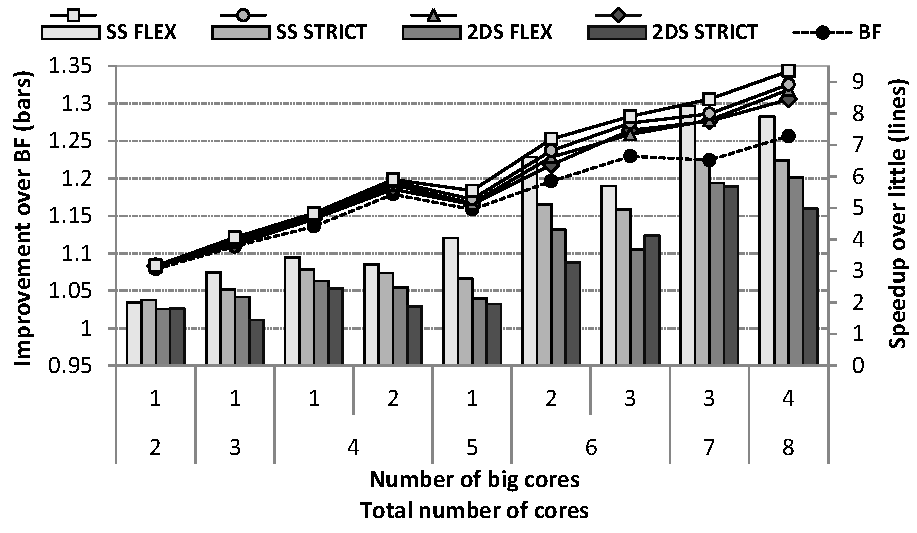
\includegraphics[width=\textwidth]{figures/cholesky_8x8_CATS.pdf}
%		\caption{Cholesky 8$\times$8}
%		\label{cholesky8x8_real}
%	\end{subfigure}
%	\begin{subfigure}[b]{0.45\textwidth}
%		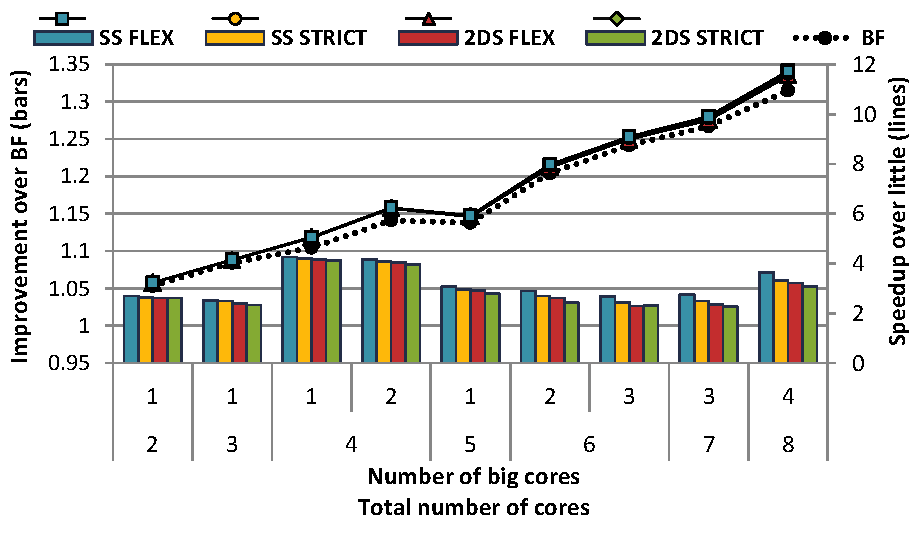
\includegraphics[width=\textwidth]{figures/cholesky_16x16_CATS.pdf}
%		\caption{Cholesky 16$\times$16}
%		\label{cholesky16x16_real}
%	\end{subfigure}
%	\begin{subfigure}[b]{0.45\textwidth}
%		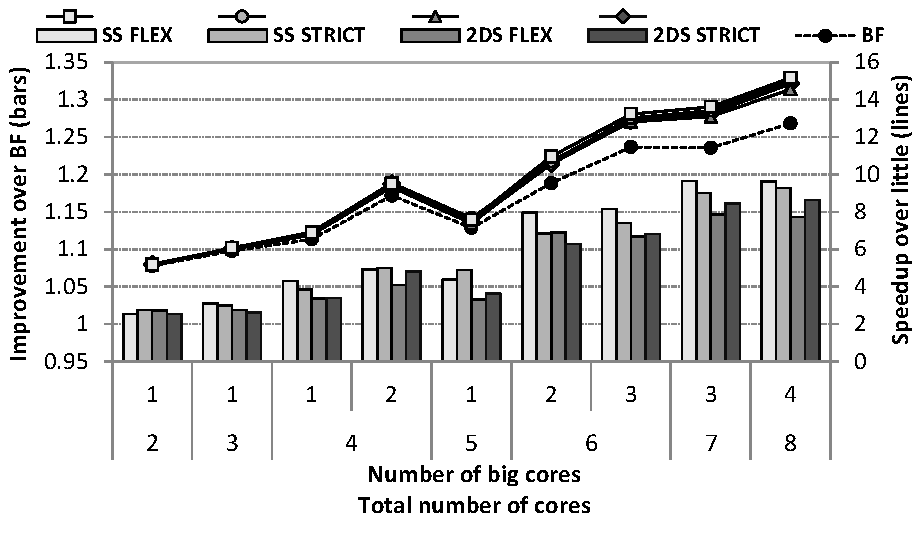
\includegraphics[width=\textwidth]{figures/QR_CATS.pdf}
%		\caption{QR}
%		\label{qr_real}
%	\end{subfigure}
%	\begin{subfigure}[b]{0.45\textwidth}
%		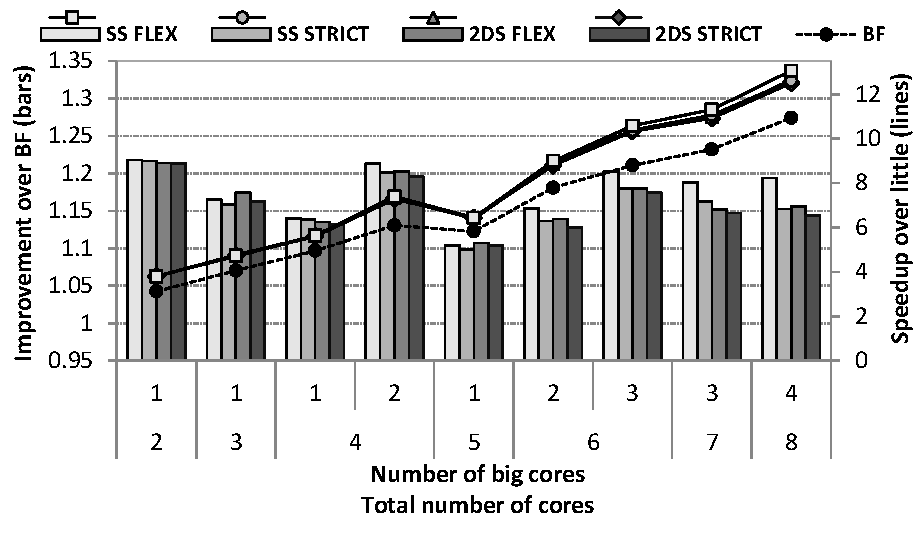
\includegraphics[width=\textwidth]{figures/heat_CATS.pdf}
%		\caption{Heat Diffusion}
%		\label{heat_ARM}
%	\end{subfigure}
%	\begin{subfigure}[b]{0.45\textwidth}
%		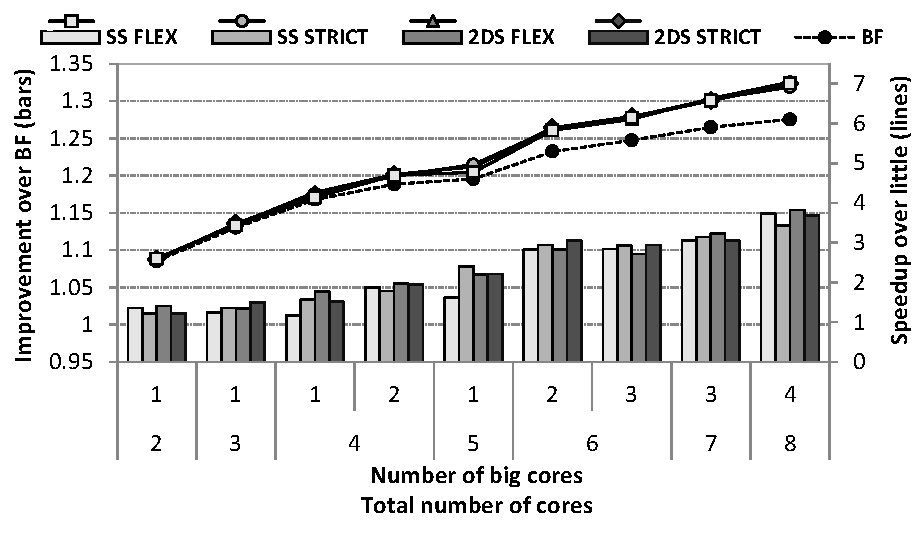
\includegraphics[width=\textwidth]{figures/intHist_CATS.pdf}
%		\caption{Integral Histogram}
%		\label{histogram_real16}
%	\end{subfigure}
%	\caption{Schedulers comparison on ODROID-XU3}
%	\label{eval_ARM}
%	\vspace{-0.4cm}
%\end{figure*}

\subsection{Real Environment Evaluation}
This subsection includes all the experiments and results obtained from the real asymmetric system ODROID-XU3.
It includes one section that explores the different CATS configurations and another section that compares the best CATS configuration among the rest of the schedulers.

\subsubsection{Evaluation of CATS Configurations}
\label{sec.cats_eval}
\begin{figure}[!t]
	\centering
		\subfloat[Speedup of CATS and BF compared to the ideal]{
		\includegraphics[width=0.45\textwidth]{figures/ideal_CATS.pdf}
		\label{BFlinear}
	}
	\subfloat[Cholesky 8$\times$8]{
		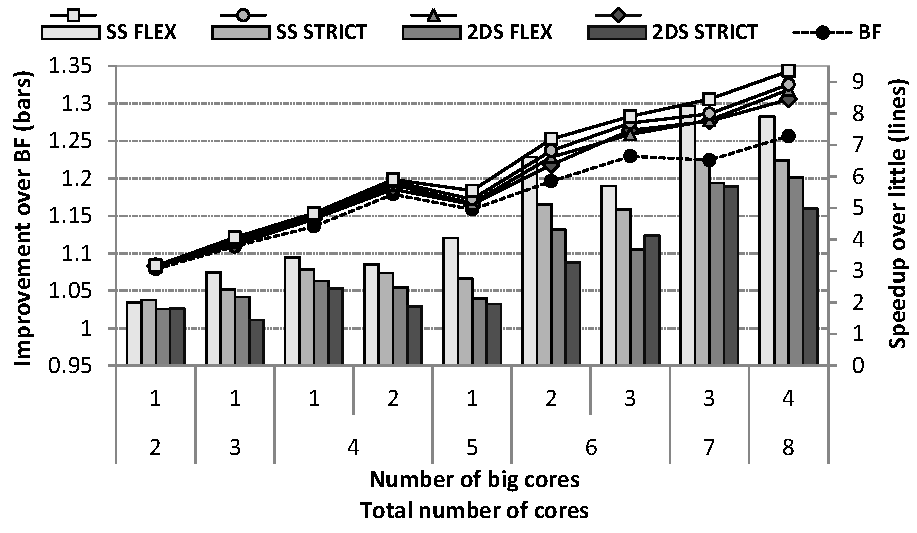
\includegraphics[width=0.45\textwidth]{figures/cholesky_8x8_CATS.pdf}
		\label{cholesky8x8_cats}
	}
	\\
	\subfloat[Cholesky 16$\times$16]{
		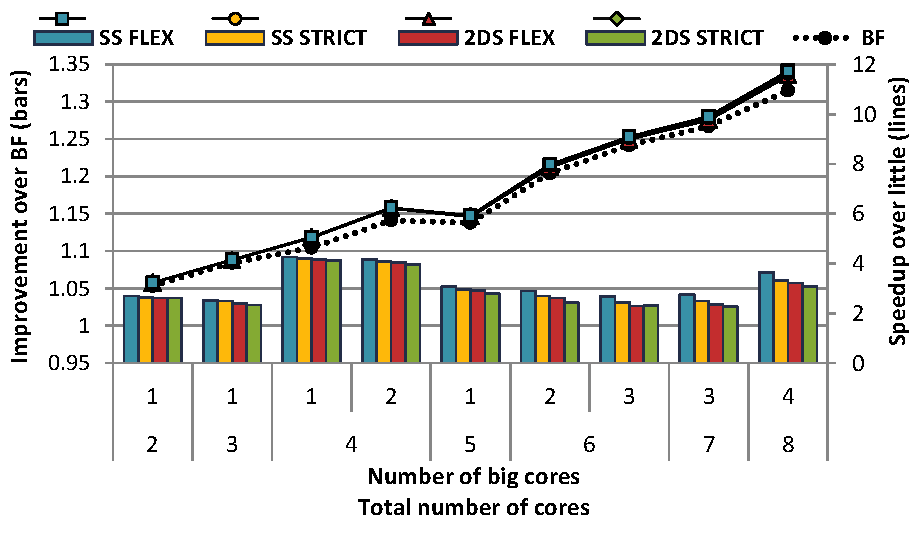
\includegraphics[width=0.45\textwidth]{figures/cholesky_16x16_CATS.pdf}
		\label{cholesky16x16_cats}
	}
	\subfloat[QR]{
		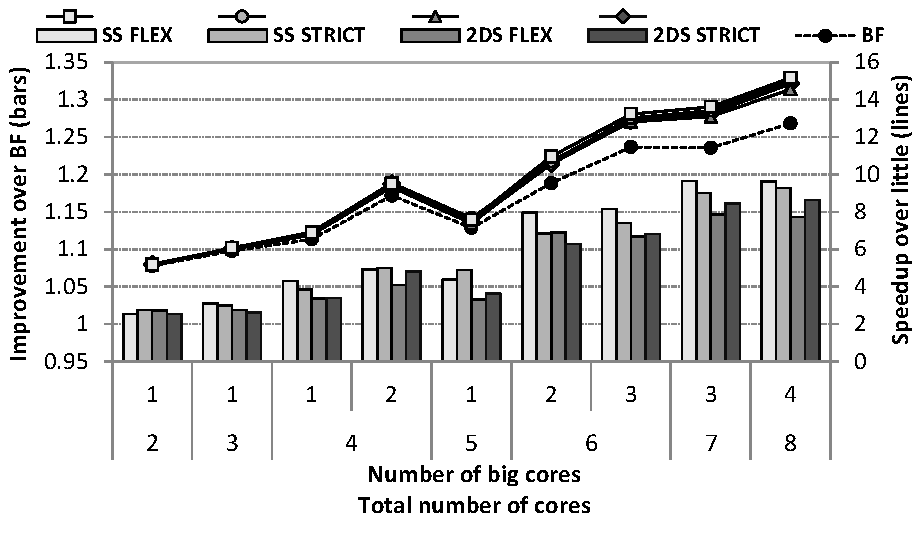
\includegraphics[width=0.45\textwidth]{figures/QR_CATS.pdf}
		\label{qr_cats}
	}
	\\
	\subfloat[Heat diffusion]{
		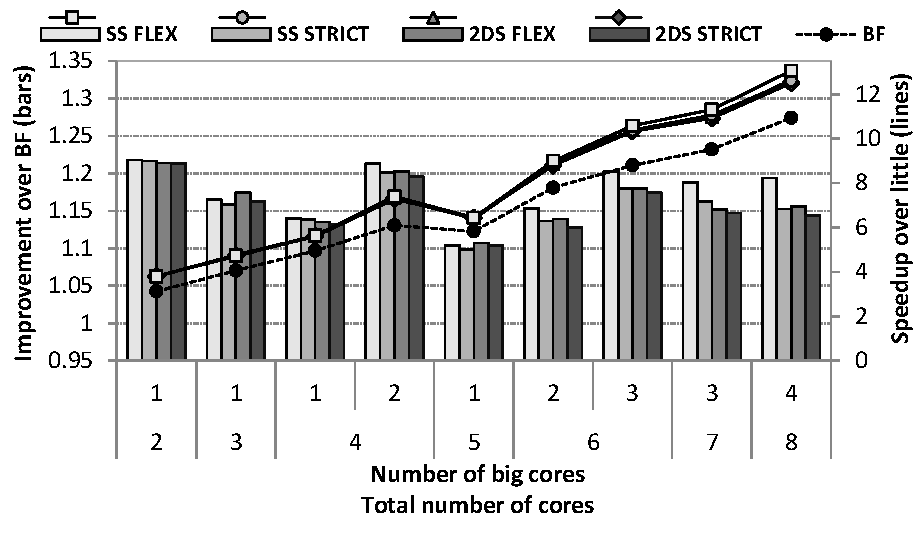
\includegraphics[width=0.45\textwidth]{figures/heat_CATS.pdf}
		\label{heat_cats}
	}
	\subfloat[Integral Histogram]{
		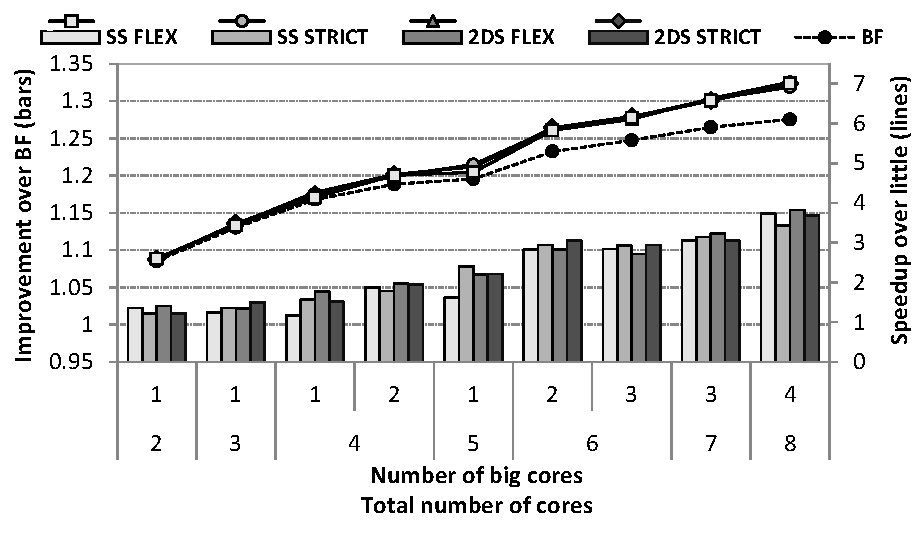
\includegraphics[width=0.45\textwidth]{figures/intHist_CATS.pdf}
		\label{histogram_cats}
	}
	%  \vspace{-0.2cm}
	\caption{Schedulers comparison on ODROID-XU3}
	%\vspace{-0.5cm}
\end{figure}
Figure~\ref{cholesky8x8_cats} shows the improvement of the CATS configurations over BF, and the speedup obtained with CATS and BF, for Cholesky on an 8$\times$8 blocked matrix. 
CATS consistently achieves better performance than BF and the improvement over BF increases as the number of cores is increased. 
Specifically, the improvement is observed to be up to 30\% for systems with seven and eight cores. 

Figure~\ref{cholesky16x16_cats} shows the performance on a 16$\times$16 block input matrix, where the improvement of CATS is smaller and ranges from 2 to 9\% and all schedulers perform fairly well. 
In this case the opportunities for enhancement are limited, since, according to Figure~\ref{BFLinear}, BF performance approaches the ideal speedup. 
The lower improvement in this case comes from the fact that the application is less sensitive to the critical path. 
The task graph is wider (as shown in Figure~\ref{fig.cholesky_graphs}) and, accordingly, the percentage of critical tasks is lower. 
Specifically the percentage of critical tasks for this input is limited to 5.5\% compared to the percentage observed with Cholesky 8$\times$8 that is 17.5\%. 
However, CATS still outperforms BF by 7\% when using the eight cores in the system.% and performs as good as dHEFT.

%It is interesting to note that the proportion of critical tasks, as shown in Table~\ref{tab.apps}, is lower than in the previous experiment, which leads to a lower utilization of the big cores for critical task execution.

Figure~\ref{qr_cats} shows the improvement of CATS over BF and their speedup for QR factorization. 
QR consists of double precision operations which cause the big cores to be 4.26$\times$ faster than the little cores. Thus, the ideal speedup of the system for QR is 20.1$\times$. 
CATS achieves a 15$\times$ speedup by shortening the execution of the dynamic longest path in the TDG. 
%Since dHEFT is not focusing on the longest path of the TDG, and it performs some random scheduling at the beginning of the execution in order to determine the task costs, it becomes less effective than CATS but still better than a BF.

Figure~\ref{heat_cats} shows the improvement of different CATS configurations over BF, and the speedup obtained with CATS and BF, for heat diffusion. 
%As shown in Table~\ref{tab.apps} heat diffusion consists of 5124 tasks; 5120 tasks of them are tasks of the same type and parameter size. 
%This limits the effect of dHEFT, that tries to find the earliest executor for each task in comparison to BF in which whenever a core becomes available, it retrieves a task from the ready queue. Thus, dHEFT is better than BF because it uses private ready queues for each core, thing that reduces the congestion of using only one ready queue. 
CATS consistently improves the scheduling of the asymmetric system from 15\% to 22\%, since the main criterion of scheduling is the TDG structure. 
CATS achieves a 13$\times$ speedup when using all eight cores, thus getting very close to the ideal 15.3$\times$ shown in Figure~\ref{BFLinear}.

Figure~\ref{histogram_cats} shows the improvement of CATS over BF, and the speedup obtained with CATS and BF, for integral histogram. 
The impact of CATS is again positive for all configurations, since the improvement is at least 5\% with the peak being 15\% for 8 cores. 
Experiments on larger systems show that the specific application's scalability saturates beyond 16 cores. 
This is because the intensive dependencies between tasks reduce the available parallelism that is mainly present among the diagonal-placed blocks due to the cross-weave scanning process. 
%Since dHEFT does not take into account the dependencies between tasks, the scheduling of an application with limited parallelism due to dependencies becomestrickier. 
Moreover, the performance ratio of this single-precision application is 1.7$\times$, so the ideal speedup is limited to 10.8$\times$.

An interesting observation is that for single-precision benchmarks the improvement of CATS is proportional to the percentage of critical tasks. 
Integral histogram achieves greater improvements in comparison to Cholesky 16$\times$16 because it schedules immediately more tasks to the fast cores of the system.
This is due to the fact that this benchmark has a higher percentage of critical tasks (7.32\%) compared to Cholesky 16$\times$16 that has 5.5\%. 
%according to the percentage of the critical tasks on Table \ref{tab.apps}. 
On the other hand, QR and heat diffusion show the opposite effect: QR has the largest performance ratio and a larger percentage of critical tasks than heat diffusion. 
However, heat diffusion shows higher overall improvement over the different configurations. 
We attribute this to the larger sensitivity of heat diffusion to the critical path, which allows CATS to achieve a large improvement even for a configuration of one big and one little core. 
%The dHEFT scheduler outperforms BF but struggles to handle applications with complex TDG. 
%Applications that consist of multiple instances of the same task type benefit less from dHEFT than applications that process tasks with variable costs, such as Cholesky and QR. 

In all cases, the SS FLEX configuration of CATS achieves the best performance, since it produces a decent amount of critical tasks for the big cores, fact that shortens the longest path of the TDG. 
A smaller amount of critical tasks is produced by the SS STRICT policy, which causes a slight imbalance that is fixed through the work stealing mechanism but with lower effectiveness. 
The 2DS FLEX configuration, produces the same amount of critical tasks as the SS FLEX, but the bi-directional work stealing allows little cores to steal critical tasks, which lengthens the critical path execution and directly increases overall execution time.

\subsubsection{Evaluation of CATS CPATH and HYBRID}
\begin{figure}[!t]
	\centering
	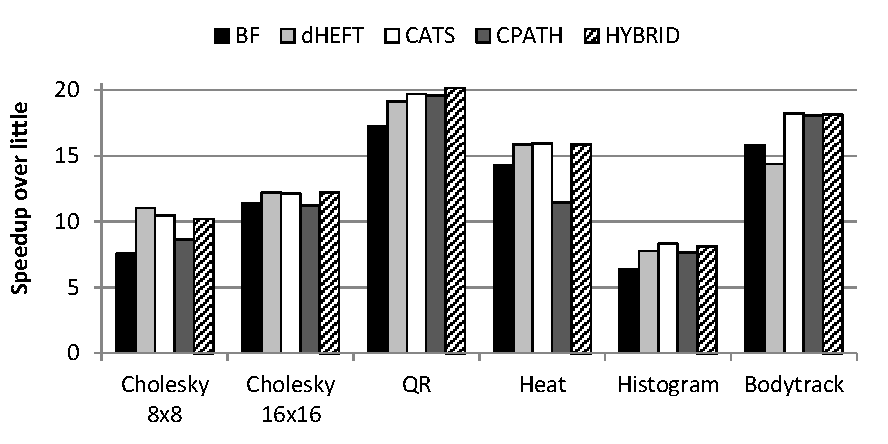
\includegraphics[width=0.7\textwidth]{images/8cores.pdf}
	\caption{Speedup of CATS, CPATH, HYBRID, dHEFT and BF on 8 cores compared to the ideal}
	\label{BFLinear}
	\vspace{-0.4cm}
\end{figure}
As it is shown in Section~\ref{sec.cats_eval}, the most efficient CATS configuration is when using the simple work stealing and flexible policy (SSFLEX).
The same applies for CPATH and HYBRID schedulers, thus the results presented in this section refer to this configuration of the schedulers. 
Figure~\ref{BFLinear} shows the speedup of CATS, CPATH, HYBRID, dHEFT and BF when running the applications on all eight cores of the Odroid-XU3. Cholesky and Integral Histogram operate on single-precision data, while QR and Heat Diffusion operate on double-precision. 
Double-precision applications get larger speedups over one little core because they benefit from a larger performance ratio when running on a big core. In the case of Bodytrack, the out-of-order processing power of the big cores helps on the efficient execution and creates a high performance ratio between big and little cores. 
For most of the cases, CATS scales better than the rest of the schedulers. 
The shortening of the critical path by running all critical tasks on big cores effectively reduces total execution time when running on all cores. 
CPATH scheduler does not achieve as high speedup as the other heterogeneous scheduling approaches but it still outperforms the baseline (BF) approach.

Figure~\ref{avg_all} shows the average speedup obtained for each scheduler and machine set-up. 
Overall, the heterogeneous schedulers outperform the platform-unaware BF scheduler.
Specifically, CATS and HYBRID achieve a higher speedup by detecting critical tasks.
We observe that their performance is approximately the same and this is due to the fact that HYBRID exploits the same CATS criticality in case the execution time of the task is not yet resolved.
CPATH is less effective due to the additional overheads of the top-to-bottom TDG traversal.
Since the evaluated dHEFT version is improved from previous studies~\cite{Chronaki:ICS2015}, it shows better performance, although it still does not reach the efficiency of CATS and HYBRID because of its task criticality agnosticism.

Moving in more detail, Figure~\ref{speedup} shows the speedup obtained for each application,  scheduler and machine set-up.
We classify the benchmarks according to their task cost variability to easier explain the results.

%------ HEAT ---------- very low variability


Heat diffusion is the kernel with the lowest task variability (e.g. the most homogeneous benchmark) as shown in Figure~\ref{heat_dist}.
CATS, HYBRID and dHEFT increase the performance of heat by 10\% on 8 cores and obtain similar results for the other numbers of cores by rearranging the tasks according to the type of the resources.
Due to its high per-task overheads shown on Table~\ref{tab.sched.apps}
%(CATS: 145.17us per task, CPATH: 748.84us per task, BF: 78.04us per task HYBRID: 170us per task)
 and the homogeneity of the benchmark, CPATH scheduler cannot outperform BF scheduler. 
Moreover, for this benchmark, CPATH detects only 23\% of the tasks to be critical while CATS and HYBRID detect approximately 54\%, when running on 8 cores.
This happens because with CPATH, it is more likely to have zero-priority tasks during the task submission step, due to the post-exit task priority assignment that the algorithm introduces. 
These tasks are considered non-critical, which limits the utilization of the big cores with CPATH. 
%the priorities of the tasks are computed more slowly with CPATH so during task submission there are many tasks with zero priority that are considered non-critical.
%Moreover, as Table~\ref{tab.critical} shows CPATH detects only 23\% of the tasks to be critical while CATS and HYBRID both detect approximately 54\% when running on 8 cores. 
%This limits the utilization of the big cores with CPATH.

%---------- CHOLESKY 16x16 ------------ low variability

Cholesky 16$\times$16 has also low task cost variability. 
The improvements of CATS, dHEFT and HYBRID over BF are limited to around 7\% when running on 8 cores.
These schedulers perform almost the same for the rest numbers of cores and CPATH performs almost the same as BF. 
The increased overheads of CPATH do not pay off with better schedules since, for the same reason as in the case of Heat diffusion, only 10\% of the tasks are marked as critical on 8 cores (while 21\% CATS and 16\% HYBRID).

%--------- BODYTRACK --------------- low variability - very high number of tasks

Bodytrack shows low task cost variability, since 99\% of its tasks have similar execution times.
In this case, contrarily to the previous benchmarks CPATH manages to achieve similar speedups to CATS and HYBRID and outperform BF by up to 15\%.
This is due to the very high number of tasks of bodytrack; CPATH overcomes its overheads by using the detected task execution times for a higher number of tasks.
In other words, the learning phase of CPATH becomes a smaller proportion of the total execution of the benchmark.
Since bodytrack has so many tasks, the per-task overhead of CPATH is around 120us while for CATS it is 93us.
On the other hand, dHEFT shows poor performance because of the overheads of analyzing a TDG with a high number of tasks to compute the earliest finish time schedule.

\begin{figure}[!tr]
	\centering
  	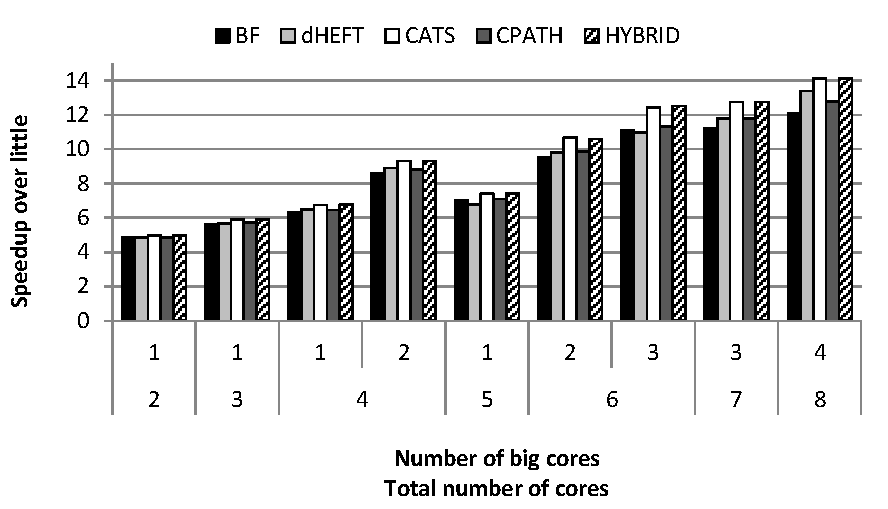
\includegraphics[width=0.7\textwidth]{images/average_all.pdf}
  	\caption{Average speedups obtained for each scheduler}
  	\label{avg_all}
  	\vspace{-0.5cm}
\end{figure}  

%---------- HISTOGRAM --------------- medium variability - good amount of tasks (2048)

Integral histogram is characterized by medium task cost variability and high amount of tasks.
This benchmark is dependency intensive with limited parallelism, which makes scheduling decisions very important.
CATS and HYBRID schedulers achieve the best results since they focus more on the TDG structure and dependencies, improving BF by 30\% and 27\% respectively.
CPATH and dHEFT are slightly less efficient and improve BF by 19 and 21\% respectively.

%---------- CHOLESKY 8x8 -------------- high variability but very few tasks

For Cholesky 8$\times$8, the heterogeneous schedulers CATS, HYBRID and dHEFT constantly improve the performance of BF and reach up to 45\% improvement on 8 cores.
It is observed here that dHEFT indeed performs better when the number of tasks is limited as this workload has 120 tasks in total.
The additional overheads of CPATH do not compensate with increased performance in this case because there are not enough tasks to apply the better scheduling.

%---------------- QR ------------ the highest variability and good number of tasks (1496)

QR factorization is the highest task cost variability benchmark as shown in Figure~\ref{qr_dist}.
This is the reason why HYBRID gradually outperforms CATS as we increase the number of cores.
With a small additional overhead,
%(CATS: 1419us while HYBRID: 14514us per-task overhead)
as Table~\ref{tab.sched.apps} shows, HYBRID manages to detect critical tasks that reside on the critical path and boost their execution reaching 17\% improvement over the baseline.
For this benchmark, CPATH also reaches a 13\% improvement over BF since task cost matters in this case. 
However, CPATH speedup is still limited compared to HYBRID because of the higher scheduling overheads which in this case is 1.8$\times$ higher than CATS overheads.
dHEFT also improves BF by finding the earliest executor of each task, but the improvement is limited to 11\% which is lower than the other approaches.
\begin{figure*}[!t]
	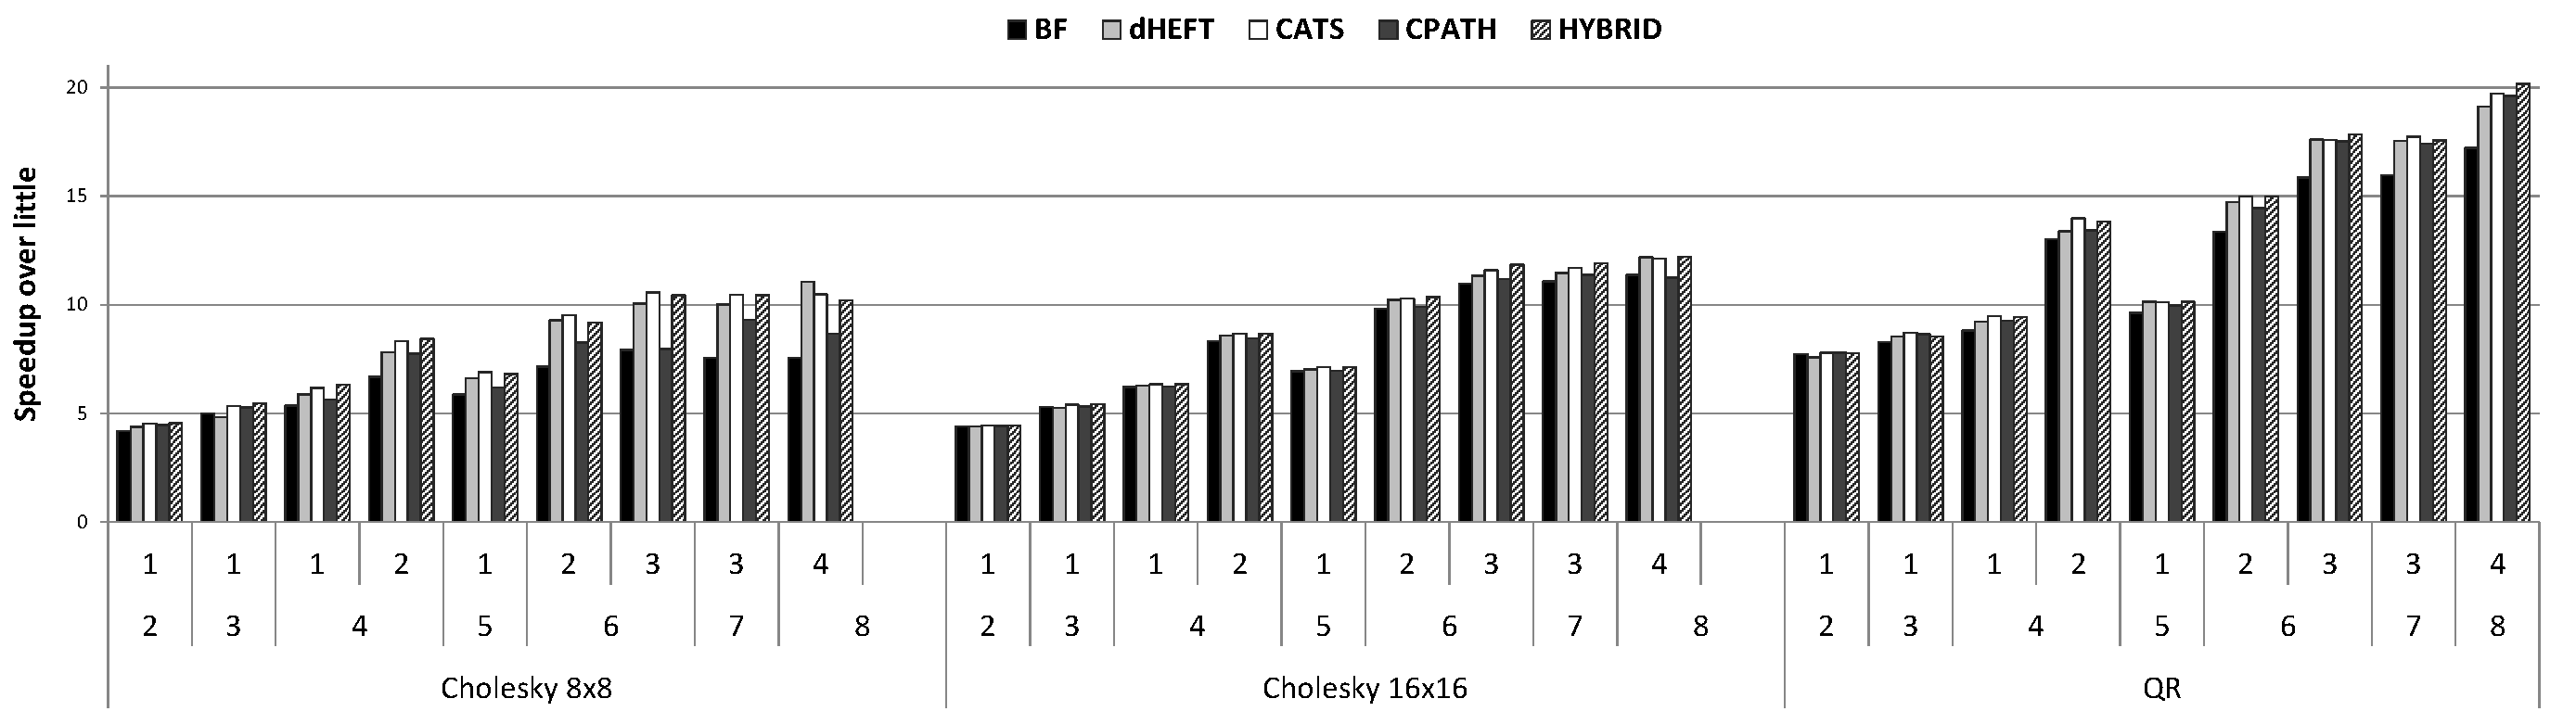
\includegraphics[width=\textwidth]{images/speedup_apps1.pdf}
	\vspace{-0.4cm}
	
	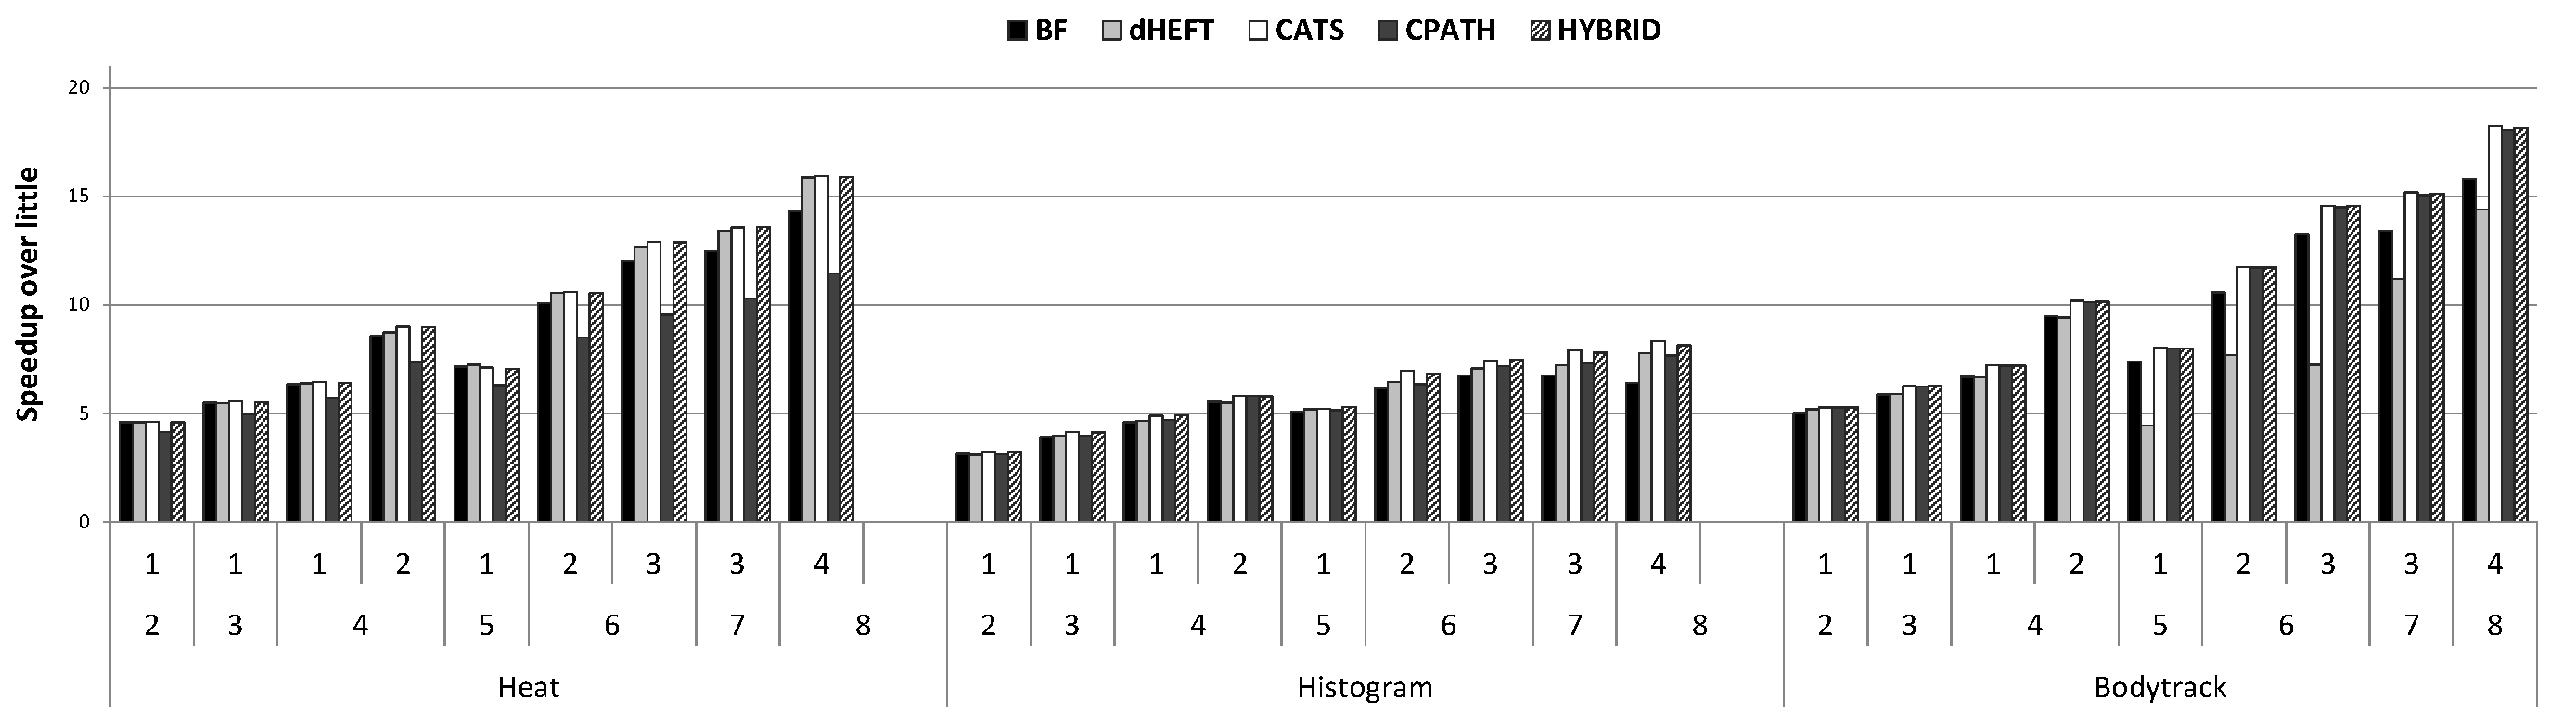
\includegraphics[width=\textwidth]{images/speedup_apps2.pdf}
	\caption{Speedups obtained for each scheduler and each application}
	\label{speedup}
	\vspace{-0.4cm}
\end{figure*}  

%--------- SUMMARY ---------------

This section showed a straight comparison between different heterogeneous schedulers.
It is important to note that schedulers like CPATH and HYBRID, that detect the time-based critical path, are the best choices when the application has a large amount of tasks.
This is because the additional overheads of these schedulers for critical path computation take place only when there are new tasks on the TDG or when there is a task exit of an untracked tt-is. 
When the TDG has been completely created, and as soon as the cost of every tt-is of the application has been tracked, the schedules of these approaches are purely beneficial.
On the other hand, schedulers like dHEFT perform the same steps for every single task that becomes ready, affecting the entire execution since the exit of a task triggers the execution of its successors that become ready. 
Thus, as the number of tasks is increased, the additional scheduling overheads are increased when using dHEFT-like approaches.
CATS scheduler is an efficient scheduling solution for any number of tasks and task cost distributions.
The additional CATS overheads take place only during task creation and are smaller than CPATH overheads with the drawback of not considering the task execution time.
If we have to choose the best and most generic heterogeneous scheduling approach among the presented schedulers the HYBRID scheduler is the best choice, since it computes an accurate critical path only when it comes at a low cost.


\subsection{Simulations}
To estimate the impact of the heterogeneity-aware schedulers on larger systems, we run three benchmarks using the TaskSim simulator~\cite{AbstrLevels_TACO12}.
The results contain a fixed scheduling overhead for all configurations, regardless of the dynamic overheads during execution (e.g., work stealing).
We simulate Cholesky, QR and Heat diffusion.
These applications feature different levels of task cost variability and have a proper amount of tasks so that the error introduced by the static overhead assumption remains negligible (e.g., bodytrack that creates 408\,525 tasks should not be compared to a 5\,000 task benchmark and static overhead).
For Cholesky, we use an input matrix of 16384$\times$16384 floats creating 512$\times$512 blocks, which results in a 32$\times$32 blocked matrix. This is because the other Cholesky configurations do not scale to 32 cores due to the limited task number. However, the task cost variability is similar to the 16$\times$ 16 input since the task size is not modified. Integral Histogram is excluded from the simulated evaluation because it does not scale beyond 16 cores.

Figures~\ref{cholesky_ts}, \ref{qr_ts} and \ref{heat_ts} show the improvement of dHEFT, CATS, HYBRID and CPATH over BF in systems with 16 and 32 cores for Cholesky, QR and heat respectively. In these experiments, the performance ratio between fast and slow cores is set to 4.5, which is the average performance ratio among the benchmarks. The heterogeneous schedulers utilize fast cores more effectively than BF, which results in larger improvements with higher number of fast cores. 

Figure~\ref{cholesky_ts} shows the improvement of the schedulers over the baseline for Cholesky. The improvement for 16 cores is comparatively small. This is due to the increased problem size used in this experiment.
This benchmark creates a small amount of critical tasks in the 32$\times$32 input, which makes the workload less sensitive to critical tasks and limits the improvement of CATS and HYBRID to a maximum of 17\%, while CPATH and dHEFT outperform BF by up to 10\%. 

%\begin{figure*}[!t]
%\begin{subfigure}[b]{0.33\textwidth}
%  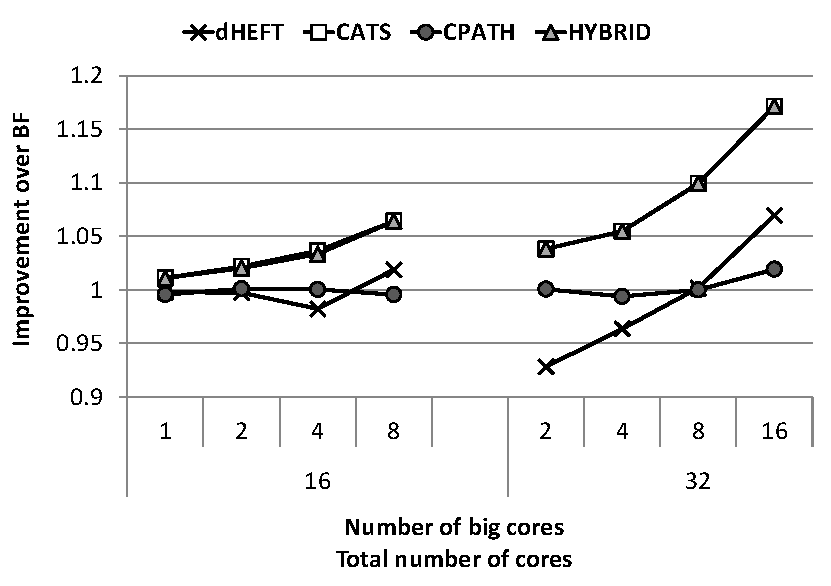
\includegraphics[width=\textwidth]{images/cholesky_TS_tall.pdf}
%  \caption{Cholesky 32$\times$32}
%  \label{cholesky_ts}
%    \vspace{-0.2cm}
%\end{subfigure}
%\begin{subfigure}[b]{0.33\textwidth}
%  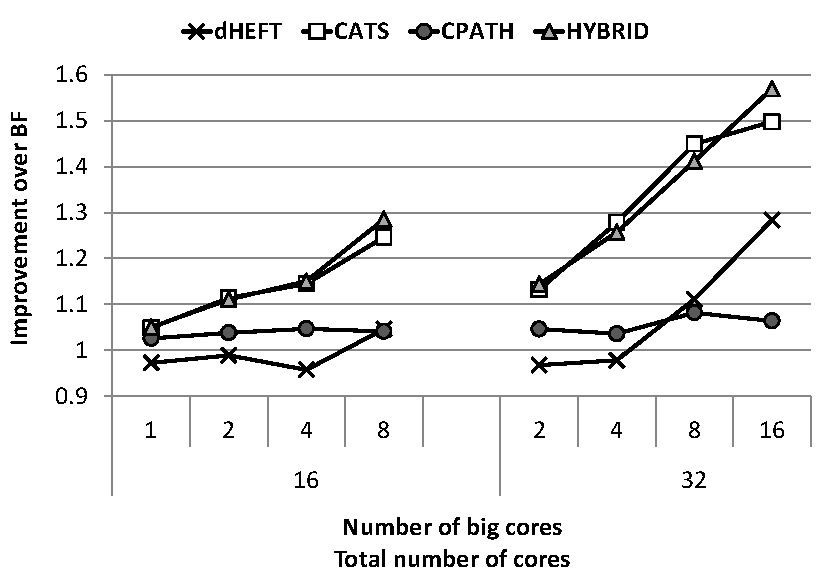
\includegraphics[width=\textwidth]{images/QR_TS_tall.pdf}
%  \caption{QR}
%  \label{qr_ts}
%    \vspace{-0.2cm}
%\end{subfigure}
%\begin{subfigure}[b]{0.33\textwidth}
%  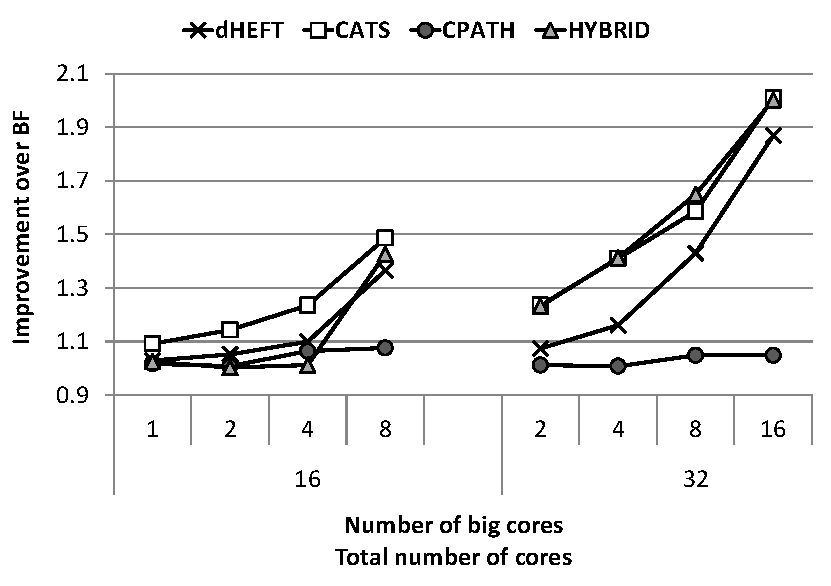
\includegraphics[width=\textwidth]{images/heat_TS_tall.pdf}
%  \caption{Heat diffusion}
%  \label{heat_ts}
%  \vspace{-0.2cm}
%\end{subfigure}  
%\caption{Improvement of heterogeneous schedulers over BF for simulated 16 and 32 core heterogeneous systems}
%\vspace{-0.5cm}
%\end{figure*}

\begin{figure}[!t]
	\centering
	\subfloat[Cholesky 32$\times$32]{
  		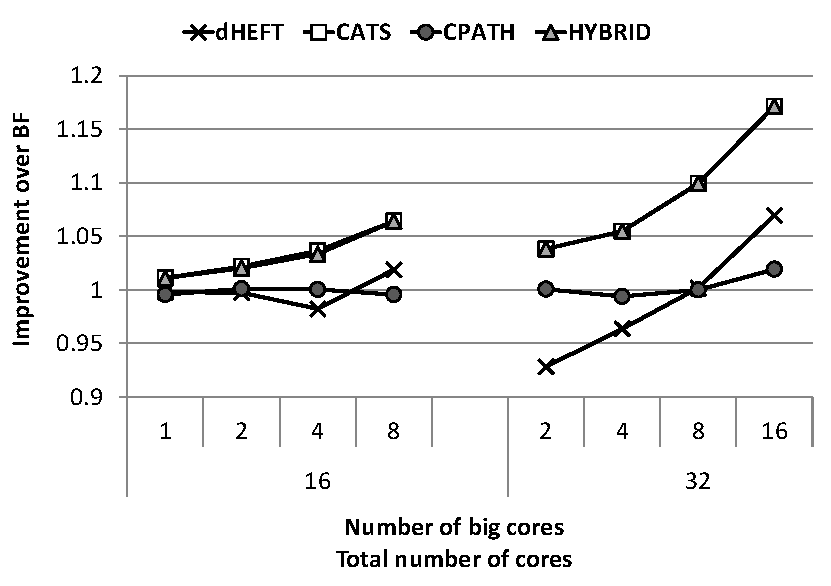
\includegraphics[width=0.65\textwidth]{images/cholesky_TS_tall.pdf}
  		\label{cholesky_ts}
	}
\\
%    \vspace{-0.2cm}
	\subfloat[QR]{
  		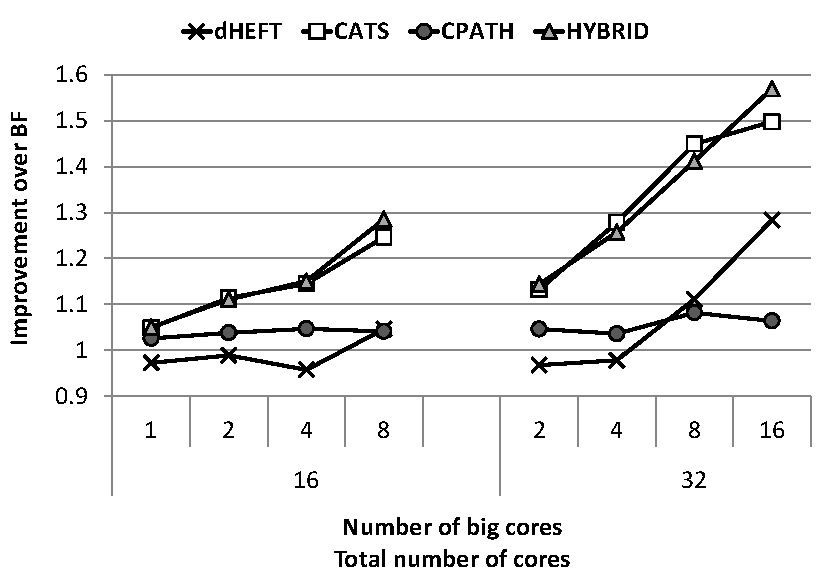
\includegraphics[width=0.65\textwidth]{images/QR_TS_tall.pdf}
  		\label{qr_ts}
  	}
\\
    %\vspace{-0.2cm}
	\subfloat[Heat diffusion]{
  		\includegraphics[width=0.65\textwidth]{images/heat_TS_tall.pdf}
  		\label{heat_ts}
  	}
%  \vspace{-0.2cm}
	\caption{Improvement of heterogeneous schedulers over BF for simulated 16 and 32 core heterogeneous systems}
%\vspace{-0.5cm}
\end{figure}

Figure~\ref{qr_ts} shows that the best option for QR, the application with the highest task cost variability, on systems with 16 or 32 cores is the HYBRID scheduler, as was also shown in the real platform evaluation, bringing improvements of 30 and 56\%.
CATS also performs well but CPATH falls short in detecting an appropriate amount of critical tasks which makes the little cores overloaded and the big cores waste their resources in work stealing.

For heat diffusion, Figure~\ref{heat_ts} shows that CATS achieves the best results outperforming BF by a factor of 2$\times$. Moreover, HYBRID achieves similar results as it performs similar schedules as CATS. However, CPATH fails to achieve optimal results because it overloads the big cores during the learning phase while the little cores remain under-utilized.


%Depending on the system and according to the application, the optimal solution for this can be found and utilize such systems effectively.


%%%%%%%%%%%%%%%%%%%%
%%%%%%%%%%%%%%%%%%%%
\section{Related Work}
\label{sec:related}
The search for efficient task scheduling on multi-core systems has been intensively studied. Most scheduling heuristics target homogeneous multiprocessors, nevertheless there is an important number of studies in heterogeneous multiprocessors. In this section we give an overview of different categories of heterogeneous schedulers
% for heterogeneous systems
%, we explain some details about schedulers targeting specific systems using compute accelerators 
and explain details of previous works on criticality-aware schedulers.

%\textit{Schedulers for Heterogeneous Systems}
\textbf{Schedulers for Heterogeneous Systems: }
There are previous works on schedulers for heterogeneous systems that form four different types of schedulers: listing, clustering, guided-random, and duplication-based schedulers.

%do not consider the criticality of tasks~\cite{Hetero95, Dyn05, Gen07,Chemical, HEFT, Dup09}. These heuristics

Listing schedulers~\cite{List, DCPS, LDCP, HEFT, CrPathDup, Li2,Li5} have two scheduling stages. In the first stage, each task is given a priority based on the policy defined in each algorithm. In the second stage, tasks are assigned to processors depending on their priorities. Most criticality-aware schedulers fall in this category, and we discuss them in Section~\ref{sec.relwork_critical}. The scheduler proposed in this paper is also a list scheduler.

Clustering schedulers~\cite{Hypertool, DSC, DCPS, Hetero95} first separate tasks into clusters, where each cluster is to be executed on the same processor. During the clustering stage, the algorithm assumes an unlimited number of available processors in the system. If the number of clusters exceeds the number of available cores, the \textit{merging} stage joins multiple clusters so that they match the number of available processors. An example is the Levelized Min Time~\cite{Hetero95} clustering scheduler. This heuristic clusters tasks that can execute in parallel according to their \textit{level} (i.e. sibling nodes in a graph have the same level), and assigns priorities to the tasks in a cluster according to their cost, (i.e. tasks with the highest cost have the highest priority). The task-to processor assignment is done in decreasing order of priority.

Guided-random schedulers randomize their schedules by applying policies influenced by other sciences. Genetic algorithms~\cite{Gen07} group tasks into generations and schedule them according to a randomized genetic technique. Chemical reaction algorithms~\cite{Chemical, LiChemical} mimic molecular interactions to map tasks to processors. Some of these guided-random approaches are designed for heterogeneous systems~\cite{Gen07, Chemical}. The scheduler by Page et al.~\cite{Dyn05} enables dynamic scheduling of multiple-sized tasks for heterogeneous systems, but it lacks support of inter-task dependencies.

Duplication-based schedulers~\cite{Dup03, Dup11, Dup09} aim to eliminate communication costs between processors by scheduling tasks and their successors on the same processor. If a task has many successors, it is duplicated and executed in multiple cores prior to its successors to reduce communication costs.
%all successor tasks get the data from their predecessors with the lowest communication cost. 
This scheduling may introduce redundant task duplications tasks which may lead to bad schedules. The Heterogeneous Economical Duplication scheduler~\cite{Dup09} performs task duplication cautiously as it removes the redundant duplicates if they do not affect performance. 

These previous works schedule tasks statically and assume the prior knowledge of the task execution times on the different processor types in the heterogeneous system.

\if 0
\subsection{Schedulers for Compute Accelerators}

The schedulers in the previous section target the scheduling of generic TDGs on generic heterogeneous architectures. In this section we cover schedulers that target specific systems with compute accelerators. These works are more focused on the scheduling of tasks on the target platform based on the abstractions provided by the corresponding mixture of programming models for the general-purpose processors and the compute accelerators in the system.

Most heterogeneous systems with compute accelerators nowadays combine general-purpose CPUs and GPU compute accelerators. There is a set of programming models providing abstractions to ease the development of applications on these platforms. OmpSs~\cite{OmpSs_PPL11, OmpSs} offers this abstraction by allowing multiple implementations of a given task to be executed on different processing units~\cite{Judit}. The scheduler then assigns the execution of a task to the best resource according to its earliest finish time. Another case is StarPU~\cite{starpu}, a library that offers runtime heterogeneity support and provides priority schedulers for task-to-processor allocation. AHP~\cite{AHP} is another framework that generates software pipelines for heterogeneous systems and schedules tasks to their earliest executor, based on profiling information gathered prior to runtime.

None of these works, however, take into account the criticality of tasks regarding task dependencies, but they rather focus on the earliest execution time of individual tasks on the processor types in the specific system configuration.
\fi

%\subsection{Criticality-Aware Schedulers}
\label{sec.relwork_critical}
\textbf{Criticality-Aware Schedulers: }
Several previous works propose scheduling heuristics that focus on the critical path of a TDG to reduce total execution time~\cite{DCPS, LDCP, HEFT, CrPathDup, Moschakis2015}. To identify the tasks on the critical path, most of these works use the concept of \textit{upward rank} and \textit{downward rank}. The upward rank of a task is the maximum sum of computation and communication cost of the tasks in the dependency chains from that task to an exit node in the graph. The downward rank of a task is the maximum sum of computation and communication cost of the tasks in the dependency chain from an entry node to that task. Each task has an upward rank and downward rank for each processor type in the heterogeneous system, as the computation and communication costs differ across core types.

The Heterogeneous Earliest Finish Time (HEFT) algorithm~\cite{HEFT} maintains a list of tasks sorted in decreasing order of their upward rank. At each schedule step, HEFT assigns the task with the highest upward rank to the processor that finishes the execution of the task at the earliest possible time. Another work is the Longest Dynamic Critical Path (LDCP) algorithm~\cite{LDCP}. LDCP also statically schedules first the task with the highest upward rank on every schedule step. The difference between LDCP and HEFT is that LDCP updates the computation and communication costs on multiple processors of the scheduled task by the costs discovered in the processor to which it was assigned.

The Critical-Path-on-a-Processor (CPOP) algorithm~\cite{HEFT} also maintains a list of tasks sorted in decreasing order as in HEFT, but in this case it is ordered according to the addition of their \textit{upward rank} and \textit{downward rank}. The tasks with the highest \textit{upward rank + downward rank} belong to the critical path. On each step, these tasks are statically assigned to the processor that minimizes the critical-path execution time.

%The drawback of static listing algorithms is the static priority assignment can lead to wrong schedules at runtime~\cite{DCP}. 

The main weaknesses of these works are that (a) they assume prior knowledge of the computation and communication costs of each individual task on each processor type, (b) they operate statically on the whole TDG, so they do not apply to dynamically scheduled applications where only a part of the TDG is available at any given time, and (c) most of them use synthetic TDGs that are not necessarily representative of the dependencies in real workloads.

%These algorithms assume the prior knowledge of the execution time of each task in the task dependency graph. Moreover, they use static scheduling, namely the computation of the critical path and task-to-processor allocation are decided before the execution of the program. This can lead to wrong predictions of the critical path which, in practice, changes during runtime.





%%%%%%%%%%%%%%%%%%%
%%%%%%%%%%%%%%%%%%%
\section{Conclusions}
\label{sec:conclusions}

\section{Conclusions}
\label{sec.scheduling.conclusions}
We introduced the first critical-path-aware dynamic scheduler for heterogeneous systems as well as the first hybrid criticality-aware scheduler. Like CATS and contrary to previous works on criticality-aware scheduling that use synthetic TDGs and require prior knowledge of profiling information, our proposals work on real platforms with real applications and do not require off-line profiling.
%, they are implementable and work without the need of profiling.

We implemented and evaluated our scheduling proposals in the runtime system of the OmpSs programming model.
We showed that even if the accuracy of CPATH is higher in terms of task criticality identification, it does not always increase performance. 
Factors like the number of tasks and task cost variability play an important role on choosing the most appropriate scheduling policy and improve the performance of task-based applications.
The implementations shown in this paper will be included in the next stable release of the OmpSs programming model. 
Furthermore, the described policies are expected to be applicable to other task-based programming models with support for task dependencies. 
%The presented schedulers assume two core types.
%by manually choosing the cores that would act as fast, which limits the scheduling effect.
%To improve this, the schedulers can be modified to assign different levels of criticality to the tasks and let the cores, according to their type, execute the tasks with the corresponding criticality level.

%After determining the critical path, the scheduler could also consider the second, third etc. longest paths and insert their tasks in the corresponding ready queues. 
%The user has to specify which cores are considered as fast for the effective execution of the critical tasks. 
%We implemented and evaluated our criticality-aware task scheduler in the runtime system of the OmpSs programming model getting satisfactory results. The implementation shown in this paper will be included in the next stable release of OmpSs. Furthermore, there are no restrictions on applying our policy to other task-based programming models with support for task dependencies. 
    
%From our experiments on a real heterogeneous multi-core platform, we found a consistent performance improvement over the default breadth-first scheduling policy and a dynamic implementation of Heterogeneous Earliest Finish Time. The improvement of our proposal, which in most cases ranges from 10 to 20\% and reaches up to 30\%, is larger as we increase the number of cores. This gives a positive projection for CATS, as it is expected that the number of cores in multi-cores will increase throughout future generation designs.

%From our simulation experiments, we found out that the improvement of CATS increases over the baseline with larger differences of performance among fast and slow cores. We explored performance ratios between two and four times faster fast cores over slow cores, with improvements ranging from 30\% to 170\%. 

In conclusion, this chapter showed the potential of different heterogeneous schedulers to speed up dependency-intensive applications and take advantage of the asymmetric compute resources.


%For future work, we aim to extend the scheduling policy to be adaptive so it can dynamically adjust its flexibility and work stealing policy depending on the application characteristics and availability of resources at runtime.

%, and dynamically adapt its configuration to the one that best fits this combination.




%\chapter{Runtime Overheads Migration}
\newcommand{\proposal}{TaskGenX}
\chapter{Runtime Overheads Migration}
%%%%%%%%%%%%%%%%%%%
%%%%%%%%%%%%%%%%%%%
\section{Introduction}
\label{sec:intro}

%%%%%%%%%%%%%%%%%%%%%%%%%%%
%%%%%%%%%%%%%%%%%%%%%%%%%%%
Since the end of Dennard scaling~\cite{Dennard74} and the subsequent stagnation of CPU clock frequencies, computer architects and programmers rely on multi-core designs to achieve the desired performance levels.
While multi-core architectures constitute a solution to the CPU clock stagnation problem, they bring important challenges both from the hardware and software perspectives.
On the hardware side, multi-core architectures require sophisticated mechanisms in terms of coherence protocols, consistency models or deep memory hierarchies. 
Such requirements complicate the hardware design process.
On the software side, multi-core designs significantly complicate the programming burden compared to their single-core predecessors.
The different CPUs are exposed to the programmer, who has to make sure to use all of them efficiently, as well as using the memory hierarchy properly by exploiting both temporal and spatial locality.
This increasing programming complexity, also known as the Programmability Wall~\cite{Chapman2007}, has motivated the advent of sophisticated programming paradigms and runtime system software to support them.

Task-based parallelism~\cite{Blumofe:PPoPP1995, Reinders2007, Bauer2012, OmpSs} has been proposed as a solution to the Programmability Wall and, indeed, the most relevant shared memory programming standards, like OpenMP, support tasking constructs~\cite{OpenMP4.0:Manual2015}.
The task based model requires the programmer to split the code into several sequential pieces, called tasks, as well as explicitly specifying their input and output dependencies. 
%It also requires these pieces of code to be annotated in terms of input or output data dependencies.
The task-based execution model (or runtime system) consists of a master thread and several worker threads. The master thread goes over the code of the application and creates tasks once it encounters source code annotations identifying them. 
The runtime system manages the pool of all created tasks and schedules them across the threads once their input dependencies are satisfied.
To carry out the task management process, the parallel runtime system creates and maintains a Task Dependency Graph (TDG).
In this graph nodes represent tasks and edges are dependencies between them.
Once a new task is created, a new node is added to the TDG. 
The connectivity of this new node is defined by the data dependencies of the task it represents, which are explicitly specified in the application's source code.
When the execution of a task finalizes, its corresponding node is removed from the TDG, as well as its data dependencies.

This task-based runtime system constitutes of a software layer that enables parallel programmers to decouple the parallel code from the underlying parallel architecture where it is supposed to run on.
As long as the application can be decomposed into tasks, the task-based execution model is able to properly manage it across homogeneous many-core architectures or heterogeneous designs with different core types. 
A common practice in the high performance domain is to map a single thread per core, which enables the tasks running on that thread to fully use the core capacity. 
Finally, another important asset of task-based parallelism is the possibility of automatically managing executions on accelerators with different address spaces. 
Since the input and output dependencies of tasks are specified, the runtime system can automatically offload a task and its dependencies to an accelerator device (e.g., GPU) without the need for specific programmer intervention~\cite{Bueno:IPDPS2012}.
Additional optimizations in terms of software pre-fetching~\cite{Papaefstathiou2013} or more efficient coherence protocols~\cite{Manivannan2014} can also be enabled by the task-based paradigm.

Despite their advantages, task-based programming models also induce computational costs.
For example, the process of task creation requires the traversal of several indexed tables to update the status of the parallel run by adding the new dependencies the recently created tasks bring, which produces a certain overhead.
Such overhead constitutes a significant burden, especially on architectures with several 10's or 100's of cores where tasks need to be created at a very fast rate to feed all of them.
This paper proposes the Task Generation Express ({\proposal}) approach. 
Our proposal suggests that the software and hardware are designed to eliminate the most important bottlenecks of task-based parallelism without hurting their multiple advantages. 
This paper focuses on the software part of this proposal and draws the requirements of the hardware design to achieve significant results.
%This paper proposes the Task Generation Express ({\proposal}) approach, a combined hardware-software solution to eliminate the most important bottlenecks of task-based parallelism without hurting their multiple advantages.
In particular, this paper makes the following contributions beyond the state-of-the-art:

\begin{itemize}

\item A new parallel task-based runtime system that decouples the most costly routines from the other runtime activities and thus enables them to be off-loaded to specific-purpose helper cores.

\item A detailed study of the requirements of a specific-purpose helper core able to accelerate the most time consuming runtime system activities. 
%To accelerate the time consuming runtime parts,
%\item A specific-purpose helper core able to accelerate the most time consuming runtime system activities. This hardware is also able to run user-level tasks, although it does so in a very slow way compared to a general purpose core.

\item A complete evaluation via trace-driven simulation considering 11 parallel OpenMP codes and $25$ different system configurations, including homogeneous and heterogeneous systems. %and large core counts up to $XXX$ cores. 
Our evaluation demonstrates how {\proposal} achieves average speedups of $3.1\times$ when compared against currently use state-of-the-art approaches.

\end{itemize} 

The rest of this chapter is organized as follows: 
Section~\ref{sec.taskgenx.background} describes the task-based execution model and its main bottlenecks.
Section~\ref{sec.taskgenx.ram} describes the new task-based runtime system this paper proposes as well as the specialized hardware that accelerates the most time-consuming runtime routines.
Section~\ref{sec.taskgenx.evaluation} describes the evaluation of {\proposal} via trace-driven simulation and Section~\ref{sec.taskgenx.conclusions} concludes this work.




%%%%%%%%%%%%%%%%%%%
%%%%%%%%%%%%%%%%%%%
\section{Background and Motivation}
\label{sec:background}
\lstset{basicstyle=\small\ttfamily,
        emphstyle=\bfseries,
        columns=fixed,
        numbers=left,xleftmargin=2em,frame=single,framexleftmargin=1.5em,
        moredelim=*[l][\textit]{//},
        moredelim=*[l][\bfseries]{\#},
        literate={...}{\dots}3
} 
\subsection{Task-based Programming Models}
\label{sec.background}
\begin{lstlisting}[float, emph={void,if,return,Dependency,DepList,Data,not,true,and,break}, captionpos=b, caption={Compiler generated pseudo-code equivalence for task annotation.},label=task_clause, emph={[2]mat}, emphstyle={[2]}, aboveskip={0\baselineskip}, frame=tb, belowskip={0\baselineskip}]
     ...
  //task_clause
  memalloc(&task, args, size);
  createTask(deps, task, parent, taskData);
     ...
\end{lstlisting}
\begin{lstlisting}[float, emph={is, void,if,return,Dependency,DepList,Data,Task,not,true,and,break}, captionpos=b, caption={Pseudo-code for task creation.},label=taskCreation, emph={[2]mat}, emphstyle={[2]}, aboveskip={0\baselineskip}, frame=tb, belowskip={0\baselineskip}]
void createTask(DepList dList, Task t,  
                Task parent, Data args) {
  initAndSetupTask(task1, parent, args);
  insertToTDG(dList, task1);
}
\end{lstlisting}

Task-based parallel programming models ~\cite{Blumofe:PPoPP1995, Reinders2007, Bauer2012, OmpSs},  are widely used to facilitate the programming of parallel codes for multi-core systems.
These programming models offer annotations that the programmer can add to the application's sequential code.
One type of these annotations is the task annotations with dependency tracking which OpenMP~\cite{OpenMP} supports since its 4.0 release~\cite{OpenMP4.0:Manual2015}. 
By adding these annotations, the programmer decomposes the application into \textit{tasks} and specifies the input and output data dependencies between them. 
A compiler is responsible to translate the annotations into code by adding calls to the programming model's runtime system. 
The runtime system consists of software threads and is responsible for the efficient execution of the tasks with respect to the data dependencies as well as the availability of resources.

When the compiler encounters a task annotation in the code, it transforms it to the pseudo-code shown in Listing~\ref{task_clause}.
\texttt{Memalloc} is performing the memory allocation for the task and its arguments.
Next is a runtime call, which is the \texttt{createTask}, responsible for the linking of the task with the runtime system.
At this point a task is considered \textit{created} and below are the three possible states of a task inside the runtime system:
\begin{itemize}
\item \textit{Created:} A task is initialized with the appropriate data and function pointers and it is inserted in the Task Dependency Graph (TDG). The insertion of a task in the TDG implies that the data dependencies of the tasks have been identified and the appropriate data structures have been created and initialized. 
%At this point a task is considered as \textit{created} but not \textit{ready}.
%\item \textit{TDG Submission:} After the allocation, a task is being inserted in the Task Dependency Graph (TDG). The insertion of a task in the TDG implies that the data dependencies of the tasks have been identified and the appropriate data structures have been created and properly initialized. At this point a task is considered as \textit{created} but not \textit{ready}.
\item \textit{Ready:} When all the data dependencies of a created task have been satisfied, the task is ready and it is inserted in the \textit{ready queue} where it waits for execution. 
\item \textit{Finished:} When a task has finished execution and has not been deleted yet.
\end{itemize}

The runtime system creates and manages the software threads for the execution of the tasks. 
Typically one software thread is being bound to each core. 
One of the threads is the \textit{master thread}, and the rest are the \textit{worker threads}. 
The master thread starts executing the code of Listing~\ref{task_clause} sequentially. 
The allocation of the task takes place first.
What follows is the task creation, that includes the analysis of the dependencies of the created task and the connection to the rest of the existing dependencies.
Then, if there are no task dependencies, which means that the task is \textit{ready}, the task is also inserted in the ready queue and waits for execution.
\begin{lstlisting}[float, emph={is, void,if,return,Dependency,DepList,Data,Task,not,for,true,and,break}, captionpos=b, caption={Pseudo-code for TDG insertion},label=insertTDG, emph={[2]mat}, emphstyle={[2]}, aboveskip={0\baselineskip}, frame=tb, belowskip={0\baselineskip}]
void insertToTDG(DepList dList, Task t) {
  if( dList is empty ) {
    readyQ->push(t);
    return;
  }
  Dependency entry;
  for( d in dList ) {
    entry = depMap[d.address()];
    if(entry==NULL) depMap.add(entry, t);
    if(d.accessType() == "write")
      entry.addLastWriter(t);
    if(d.accessType() == "read") {
        entry.addReader(t);
        entry.lastWriter()->addSuccessor(t);
    }
  }
}
\end{lstlisting}
Listing~\ref{taskCreation} shows the pseudo-code for the task creation step within the runtime.
The \texttt{createTask} function is first initializing the task by copying the corresponding data to the allocated memory as well as connecting the task to its parent task (\texttt{initAndSetupTask}).
After this step, the task is ready to be inserted in the TDG. 
The TDG is a distributed and dynamic graph structure that the runtime uses to keep the information about the current tasks of the application. 
The insertion of a task in the TDG is done by the \texttt{insertToTDG} function.
This function takes as arguments a list with all the memory addresses that are to be written or read by the task (\texttt{dList}), and the task itself.
Listing~\ref{insertTDG} shows the pseudo-code for the TDG insertion. 
If for a task the \texttt{dList} is empty (line 2), this means that there are no memory addresses that need to be tracked during the execution; thus, the task is marked as \textit{ready} by pushing it to the \textit{ready queue} (line 3).
Each entry of \texttt{dList} contains the actual memory address as well as the access type (read, write or read-write).
The runtime keeps a distributed unified dependency tracking structure, the \texttt{depMap} where it stores all the tracked memory addresses together with their writer and reader tasks.
For each item in the \texttt{dList} the runtime checks if there is an existing representation inside the \texttt{depMap} (line 8).
If the memory address of an entry of the \texttt{dList} is not represented in the \texttt{depMap}, it is being added as shown in line 9.
If the address of a \texttt{dList} item exists in the \texttt{depMap}, this means that a prior task has already referred to this memory location, exhibiting a data dependency.
According to the access type of \texttt{d}, the readers and the writers of the specific address are updated in the \texttt{depMap} (lines 10-15).

To reduce the lookup into the \texttt{depMap} calls, every time the contents of a memory address are modified, the tasks keep track of their \textit{successors} as well as the number of \textit{predecessors}.
The \textit{successors} of a task are all the tasks with inputs depending on the output of the current task.
The \textit{predecessors} of a task are the tasks whose output is used as input for the current task.
When a \texttt{read} access is identified, the task that is being created is added to the list of successors of the last writer task, as shown on line 20 of Listing~\ref{taskCreation}.

\begin{lstlisting}[float, emph={void,if,return,Task,for,not,true,and,break}, captionpos=b, caption={Pseudo-code for task$\_$finish runtime activity.},label=taskFinish, emph={[2]mat}, emphstyle={[5]}, aboveskip={0\baselineskip}, frame=tb, belowskip={0\baselineskip}]
void task_finish(Task *t) {
  depMap.removeReaderWriter(t);
  if(t->successors.empty()) delete t;
  else {
    for( succ in t->successors ) {
        succ.decreasePredecessors();
        if(succ.numPredecessors == 0) 
            readyQ->push(succ);
    }
  }
}
\end{lstlisting}

As tasks are executed, the dependencies between them and their successors are satisfied. 
So the successor tasks that are waiting for input, eventually become \textit{ready} and are inserted to the ready queue.
When a task goes to the \textit{finished} state, the runtime has to perform some actions in order to prepare the successor tasks for execution.
These actions are described in Listing~\ref{taskFinish}.
The runtime first updates the \texttt{depMap} to remove the possible references of the task as reader or writer (line 2).
Then, if the task does not have any successors, it can safely be deleted (line 3).
If the task has successors, the runtime traverses the successor list and for each successor task it decreases its predecessor counter (lines 5-6).
If for a successor task its predecessor counter reaches zero, then this task becomes \textit{ready} and it is inserted in the \textit{ready queue} (lines 7-8).

The runtime activity takes place at the task state changes. 
One state change corresponds to the task creation, so a task from being just allocated it becomes \textit{created}. 
At this point the runtime prepares all the appropriate task and dependency tracking data structures as well as inserts the task into the TDG.
The second change occurs when a task from being \textit{created} it becomes \textit{ready};
this implies that the input dependencies of this task are satisfied so the runtime schedules and inserts the task into the ready queue.
The third change occurs when a running task finishes execution. 
In this case, following our task states, the task from being \textit{ready} it becomes \textit{finished}; this is followed by the runtime updating the dependency tracking data structures and scheduling possible successor tasks that become ready. 
For the rest of the paper we will refer to the first state change runtime activity as the task creation overheads (\textit{Create}).
For the runtime activity that takes place for the following two state changes (and includes scheduling and dependence analysis) we will use the term runtime overheads (\textit{Runtime}).



%\begin{lstlisting}[float, emph={void,if,return,not,true,and,break}, captionpos=b, caption={Pseudo-code for task creation.},label=taskCreation, emph={[2]mat}, emphstyle={[2]}, aboveskip={0\baselineskip}, frame=tb, belowskip={0\baselineskip}]
%
%void createTask(Deplist dList, Task task1, 
%            Task parent, Data taskData) {
%  initAndSetupTask(task1, parent, taskData);
%  insertToTDG(dList, task1);
%}
%
%Dependency depMap[];
%
%void insertToTDG(DepList dList, Task task1) {
% if( dList.empty() ) {
%   rQueue_submission(task1);
%   return;
% }
% Dependency entry;
% for( d in dList ) {
%   entry = depMap.lookupAddress(d.address());
%   if(entry == NULL) 
%     depMap.add(d.address(), d.accessType(), task1);
%   if(d.accessType() == "write") {
%     entry.addLastWriter(task1);
%   }
%   else if(d.accessType() == "read") {
%     entry.addReader(task1);
%     entry.lastWriter()->addSuccessor(task1);
%   }
%   else if(d.accessType() == "read-write") {
%     entry.addLastWriter(task1);
%     entry.addReader(task1);
%   }
%
% }
%}
%\end{lstlisting}


\if 0
\begin{lstlisting}[float, emph={void,if,return,Dependency,DepList,Data,not,true,and,break}, captionpos=b, caption={Pseudo-code for the SRT loop.},label=SRTloop, emph={[2]mat}, emphstyle={[2]}, aboveskip={0\baselineskip}, frame=tb, belowskip={0\baselineskip}]

void TDG_submission(Task *task, Data *dependencies) {
 list tmpDeps;
 for( d in dependencies ) {
   if(d.address() == NULL) continue;
   for( t in tmpDeps ) {
     if(t.address() == d.address()) {
       t.setInput(d.isInput() || t.isInput());
       t.setOutput(d.isOutput() || t.isOutput());
       found = true;
       break;
     }
   }
   if(!found) t.push(d); 
 }
 for( t in tmpDeps ) {
   address=t.address();
   TrackableObject existing = depsMap.lookup(address);
   if( t.type == input ) 
     addDep(t, address, input);
   
 }
 
 return;
}
\end{lstlisting}
\fi

\if 0
\begin{lstlisting}[float, emph={void,if,return,rQueue_submission, not,true,and,break}, captionpos=b, caption={Pseudo-code of the task$_$finish runtime activity.},label=task_finish, emph={[2]mat}, emphstyle={[2]}, aboveskip={0\baselineskip}, frame=tb, belowskip={0\baselineskip}]

task_finish:
  if(numDeps == 0) delete task;
  for( succ in task->successors ) {
    succ.deletePredecessor(task);
    succ.decreasePredecessors();
  	if(succ.numPredecessors == 0) rQueue_submission(succ);
  }
\end{lstlisting}
\fi
\subsection{Motivation}

%\begin{figure}[t!]%
%	\centering
%	\subfigure[Figure 1]{\label{fig:sub1}\includegraphics[width=.45\linewidth]{figures/master_thread.pdf}}
%	\subfigure[Figure 1]{\label{fig:sub1}\includegraphics[width=.45\linewidth]{figures/master_thread.pdf}}
%	\caption{My caption}
%\end{figure}


\begin{figure}[t!]%
	\centering
	\includegraphics[width=0.75\columnwidth]{figures/master_thread.pdf}
	\caption{Master thread activity for Cholesky as we increase the number of cores.}
	%\caption{Performance improvements on a big.LITTLE processor with different $(F,N)$ configurations, where $F$ is the total number of big cores and $N$ the total number of cores. Results are normalized to running on four little cores with pinned Pthreads.}%
	\label{fig:master_thread}%
\end{figure}

Figure~\ref{fig:master_thread} shows the runtime activity of the master thread during the execution of the Cholesky{\footnote{Details about the benchmarks used are in Section~\ref{sec.background.applications}} benchmark on 8, 16, 32, 64 and 128 cores\footnote{The experimental set-up is explained in Section~\ref{sec.background.arm}}.
The execution time represented here is the wall clock time during the parallel region of the benchmark.
Each one of the series represents a different runtime overhead from the ones described above.
%\textit{Create} represents the \textit{Creation} step, 
%\textit{Runtime} refers to the \textit{Finish} step, \textit{Idle} shows the master thread's idle time and the \textit{Tasks} is the time spent on task execution. 
The percentage of time spent on task creation is increasing as we increase the number of cores.
This is because the creation overhead is invariant of core count: the more we reduce the application's execution time by adding resources the more important this step becomes in terms of execution time.
In contrast, the task execution time percentage is decreased as we increase the number of cores because the computational activity is being shared among more resources.
One way to reduce the task creation overhead is by introducing nested parallelism. 
In this programming technique, every worker thread is able to generate tasks thus the task creation is spread among cores and its overhead is reduced.
However, not all applications can be implemented with this parallelization technique and there are very few applications using this scheme.
\textit{Runtime} decreases as we increase the number of cores because this activity is also shared among the resources.
This is because this part of the runtime takes place once the tasks finish execution and new tasks are being scheduled. 
So the more the resources, the less the runtime activity per thread, therefore less activity for the master thread.
%\kc{explain that this is wall clock time. The \textit{Runtime} activity is actually the part of the master thread but also the worker threads are performing this activity while the Create is only within the master thread.}


Our motivation for this work is the bottleneck introduced by task creation as shown in Figure~\ref{fig:master_thread}.
Our runtime proposal decouples this piece of the runtime and accelerates it on a specialized hardware resulting in higher performance.



%%%%%%%%%%%%%%%%%%%
%%%%%%%%%%%%%%%%%%%
\section{Task Generation Express}
\label{sec:ram}
%We propose a hardware and software solution to overcome the performance bottleneck described in the previous section. 
%In our system we assume the existence of a specialized hardware that is responsible for the fast execution of the task creation. 
%To use such a hardware we need flexible software that manages to move the task creation to be executed there.

%The software that we employ uses a specialized queue for the task creation requests. 
%Each thread that is about to create a task instead of creating it, it inserts a task creation request in this queue. 
%The responsible hardware then reads the queue and executes the requests.

In this paper we propose a semi-centralized runtime system that dynamically separates the most computationally intensive parts of the runtime system and accelerates them on specialized hardware. 
To develop the {\proposal} we use the OpenMP programming model~\cite{OpenMP},~\cite{OpenMP4.0:Manual2015}.
The base of our implementation is the Nanos++ runtime system responsible for the parallel execution and it is used in this paper as a replacement of the entire OpenMP's default runtime.

Nanos++~\cite{nanos} is a distributed runtime system that uses dynamic scheduling.
As most task-based programming models, Nanos++ consists of the master and the worker threads.
The master thread is launching the parallel region and creates the tasks that have been defined by the programmer{\footnote{Nanos++ also supports nested parallelism so any of the worker threads can potentially create tasks. However the majority of the existing parallel applications are not implemented using nested parallelism.}}.
The scheduler of Nanos++ consists of a~\textit{ready queue} (\textit{TaskQ}) that is shared for reading and writing among threads and is used to keep the tasks that are ready for execution.
All threads have access to the \textit{TaskQ} and once they become available they try to pop a task from the \textit{TaskQ}.
When a thread finishes a task, it performs all the essential steps described in Section~\ref{sec.background} to keep the data dependency structures consistent.
Moreover, it pushes the tasks that become ready to the \textit{TaskQ}.

%We implement the Runtime Activity Manager ({\proposal}) on top of Nanos distributed runtime system that uses dynamic scheduling~\cite.


\subsection{Implementation}

{\proposal} relieves the master and worker threads from the intensive work of task creation by offloading it on the specialized hardware.
%{\proposal} assumes the existence of a specialized hardware that accelerates this part of the runtime.
Our runtime, apart from the master and the worker threads, introduces the Special Runtime Thread (SRT). 
When the runtime system starts, it creates the SRT and binds it to the task creation accelerator, keeping its thread identifier in order to manage the usage of it.
During runtime, the master and worker threads look for ready tasks in the task ready queue and execute them along with the runtime.
Instead of querying the ready queue for tasks, the SRT looks for runtime activity requests in the Runtime Requests Queue (\textit{RRQ}) and if there are requests, it executes them.

Figure~\ref{fig:communication} shows the communication infrastructure between threads within {\proposal}.
Our system maintains two queues; the Ready Task Queue (\textit{TaskQ}) and the Runtime Requests Queue (\textit{RRQ}).
The \textit{TaskQ} is used to keep the tasks that are ready for execution. 
The \textit{RRQ} is used to keep the pending runtime activity requests. 
The master and the worker threads can push and pop tasks to and from the \textit{TaskQ} and they can also add runtime activity to the \textit{RRQ}. 
The special runtime thread (SRT) pops runtime requests from the \textit{RRQ} and executes them on the accelerator.

When the master thread encounters a task clause in the application's code, after allocating the memory needed, it calls the \texttt{createTask} as shown in Listing~\ref{taskCreation} and described in Section~\ref{sec.background}. 
{\proposal} decouples the execution of \texttt{createTask} from the master thread. 
To do so, {\proposal} implements a wrapper function that is invoked instead of \texttt{createTask}.
In this function, the runtime system checks if the SRT is enabled; if not then the default behaviour takes place, that is, to perform the creation of the task.
If the SRT is enabled, a \textit{Create} request is generated and inserted in the \textit{RRQ}.
The \textit{Create} runtime request includes the appropriate info to execute the code described in Listing~\ref{taskCreation}.
That is, the dependence analysis data, the address of the allocated task, its parent and its arguments.



\begin{lstlisting}[float, emph={SRTloop}, caption={Pseudo-code for the SRT loop.},label=SRTloop]
void SRTloop() {
  while( true ) {   
    while(RRQ is not empty) 
      executeRequest( RRQ.pop() );
    if( runtime.SRTstop() ) break;
  }
  return; 
}  
\end{lstlisting}

While the master and worker threads are executing tasks, the SRT is looking for \textit{Create} requests in the \textit{RRQ} to execute.
Listing~\ref{SRTloop} shows the code that the SRT is executing until the end of the parallel execution.
The special runtime thread continuously checks whether there are requests in the \textit{RRQ} (line 3). 
If there is a pending creation request, the SRT calls the \texttt{executeRequest} (line 4), which extracts the appropriate task creation data from the creation request and performs the task creation by calling the \texttt{createTask} described in Listing~\ref{taskCreation}.
%executes the task submission and inserts the task in the TDG with a call to the \texttt{executeRequest} (line 4). 
When the parallel region is over, the runtime system informs the SRT to stop execution.
This is when the SRT exits and the execution finishes (line 5).

%\kc{communication:} To relieve the master and worker threads from the intensive runtime activity we use a simple queueing communication scheme that offloads the task submission on a specialized hardware.
%Whenever a thread encounters a task submission phase, instead of executing the submit call of the scheduler, it creates a runtime request and inserts it in the RRQ. 
%Concurrently, the SRT queries the RRQ for runtime requests and as long as there are requests available it executes them.
%Moreover, the SRT executes tasks whenever there are no requests for a long time to speedup the execution.


%\begin{figure}[tl]%
%	\centering
%	\includegraphics[width=0.4\columnwidth]{figures/communication2.pdf}
%	\caption{Communication mechanism between master/workers and SRT threads.}
%	\label{fig:communication}%
%	\vspace{-0.3cm}
%\end{figure}






%\section{Hardware requirements}}
%\label{sec:hw}
\subsection{Hardware Requirements}
\label{sec:hw_req}

%\begin{figure}[t]%
%	\centering
%	\includegraphics[width=0.6\columnwidth]{figures/hw_fig.pdf}
%	\caption{SoC architecture including three types of cores: out of order, in-order and RTopt.}
%	\label{fig:hw}%
%	\vspace{-0.3cm}
%\end{figure}
As described in the previous section, {\proposal} assumes the existence of specialized hardware that accelerates the task creation step. 
The goal of this paper is not to propose a detailed micro-architecture of the specialized hardware; instead we sketch the high-level hardware requirements for the {\proposal} set-up, in the hope to be an insightful and useful influence for hardware designers.
The SRT is bound to the task creation accelerator and executes the requests in the RRQ. 
Previous studies have proposed custom accelerators for the runtime activity~\cite{TaskSS, Xubin, Nexus, Swarm, TMU, Carbon}. 
These proposals significantly accelerate (up to three orders of magnitude) different bottlenecks of the runtime system\footnote{Section~\ref{sec:related} further describes these proposals.}. 
These special purpose designs can only execute runtime system activity.

%\begin{figure}[t!]%
%	\centering
%	\subfloat[Communication mechanism between master/workers and SRT threads.]{\label{fig:communication}\includegraphics[width=0.5\columnwidth]{figures/communication2.pdf}} \hspace{0.2cm}
%	\subfloat[SoC architecture including three types of cores: out of order, in-order and RTopt.]{\label{fig:hw}\includegraphics[width=0.4\linewidth]{figures/hw_fig.pdf}}
%	\caption{}
%\end{figure}

\begin{figure}[t!]%
	\centering
	
	\includegraphics[width=0.9\textwidth]{figures/communication2.pdf}
	\caption{Communication mechanism between master/workers and SRT threads.}
	\label{fig:communication}
\end{figure}
	
As an alternative, in our envisioned architecture we propose to have a general purpose core that has been optimized to run the runtime system activity more efficiently. 
The runtime optimized (RTopt) core can be combined with both homogeneous or heterogeneous systems and accelerate the runtime activity.
Figure~\ref{fig:hw} shows the envisioned architecture when RTopt is combined with an asymmetric heterogeneous system.
%Figure~\ref{fig:hw} shows the envisioned asymmetric multi-core architecture with different core types. 
This architecture has three core types that consist of simple in-order cores, fast out-of-order cores and an RTopt core for the SRT. 
RTopt can optimize its architecture, having a different cache hierarchy, pipeline configuration and specialized hardware structures to hold and process the SRT. 
As a result, the RTopt executes the SRT much faster than the other cores. 
The RTopt can also execute tasks, but will achieve limited performance compared to the other cores as its hardware structures have been optimized for a specific software (the SRT).
\begin{figure}[t!]
	\centering
	\includegraphics[width=0.6\textwidth]{figures/hw_fig.pdf}
	\caption{SoC architecture including three types of cores: out of order, in-order and RTopt.}
	\label{fig:hw}
\end{figure}
To evaluate our approach we study the requirements of the RTopt in order to provide enough performance for {\proposal}.
Based on the analysis by Etsion et al.~\cite{TaskSS}, there is a certain \textit{task decode rate} that leads to optimal utilization of the multi-core system.
This rule can be applied in the case of {\proposal} for the \textit{task creation rate}, i.e., the frequency of task generation of the runtime system.
If the \textit{task creation rate} is higher than the \textit{task execution rate}, then for a highly parallel application the resources will always have tasks to execute and they will not remain idle.
To achieve a high \textit{task creation rate}, we can accelerate the task creation cost.
Equation~\ref{eq.create} shows the maximum optimal task creation cost, $C_{opt}(x)$ in order to keep $x$ cores busy, without starving due to task creation.

%\begingroup\makeatletter\def\f@size{9}\check@mathfonts
\begin{equation}
  \text{$C_{opt}(x) = avg.\ task\ duration / x$ }
\label{eq.create}
\end{equation}
%\endgroup

If $C_{gp}$ is the cost of task creation when it is performed on a general purpose core, then the RTopt has to achieve a speedup of $r = C_{gp}/C_{opt}(x)$ to achieve full utilization of the system. 
Section~\ref{sec:experimental:simulation} performs an analysis based on these requirements for the evaluated applications. 
As we will see in Section~\ref{sec:experimental:simulation}, a modest and implementable value of $r=16\times$ is enough to significantly accelerate execution on a 512-core system.

Finally, if {\proposal} executes on a regular processor without the RTopt core, the SRT is bound to a regular core without any further modification. In this scenario, applications will not significantly benefit from having a separate SRT.




%%%%%%%%%%%%%%%%%%%
%%%%%%%%%%%%%%%%%%%

\begin{table*}[t]
\begin{center}
\caption{Evaluated benchmarks and relevant characteristics}
\label{tab.apps}
\resizebox{\textwidth}{!}{%
\begin{tabular}{|c|c|c|c|c|c|c|c|c|c|}
\hline
\multirow{3}{*}{\parbox{13mm}{\centering Application}} & 
\multirow{3}{*}{Problem size} & 
\multirow{3}{*}{\parbox{10mm}{\centering \#Tasks}} & 
\multirow{3}{*}{\parbox{17mm}{\centering Avg task CPU cycles (thousands)}} & 
\multicolumn{3}{|c|}{\parbox{22mm}{\centering Per task overheads (CPU cycles)}} & & &\\
\cline{5-7}
& & & & \multirow{2}{*}{\parbox{10mm}{\centering Create}} & \multirow{2}{*}{\parbox{9mm}{\centering All}} & \multirow{2}{*}{\parbox{11mm}{\centering Deps + Sched}} & \multirow{2}{*}{\parbox{15mm}{\centering Measured perf. ratio}} &
{\parbox{10mm}{\centering $r$}} &
\multirow{2}{*}{\parbox{11mm}{\centering Parallel model}} \\
& & & & & & & & & \\ %\hhline{~~~~~~}
\hline

\multirow{2}{*}{\parbox{18mm}{\centering Cholesky factorization}} & 
32K 256 & 357\,762  & 753 & 15221 &  73286 &  58065 &  \multirow{2}{*}{\parbox{9mm}{\centering 3.5}} & 10.34 & \multirow{2}{*}{\parbox{17mm}{\centering dependencies}}\\                                              & 32K 128 & 2829058 & 110 & 17992 &  58820 &  40828 & & 83.74 &\\
%& 32$\times$32 blocks of 512$\times$512 floats & 5984 & & 1\,551\,322 & 104.76 &  238.02 &  194.28  & \\ 
\hline{}
\multirow{2}{*}{\parbox{18mm}{\centering QR factorization}} & 16K 512 & 11\,442 & 518\,570  & 17595 & 63008 &   45413 & \multirow{2}{*}{\parbox{9mm}{\centering 6.8}} & 0.01 &\multirow{2}{*}{\parbox{17mm}{\centering dependencies}}\\
&  16K 128 & 707\,265 & 3\,558 & 21642 & 60777 & 39135 & & 3.11 &\\
\hline
Blackscholes & native & 488\,202 & 348  &   29141  &  85438 &  56297 & 2.3 & 42.87 & data-parallel \\
\hline
Bodytrack & native & 329\,123 & 383 &  9\,505 &  18979 & 9474 & 4.2 & 12.70 & pipeline \\ 
%Heat diffusion & Heat &  &  &  &  &  & \\ 
\hline
Canneal & native & 3\,072\,002 & 67 & 25781 & 50094 &  24313 & 2.0 & 197.01 & unstructured \\
\hline
Dedup & native & 20\,248 & 1\,532 & 1294 & 9647 &  8353 & 2.7 & 0.43 & pipeline \\
\hline 
Ferret & native$\times$2 & 84\,002 & 29\,088 & 38913 & 98457 &  59544 & 3.6 & 0.68 & pipeline \\
\hline
Fluidanimate & native & 128\,502 & 16\,734 & 30210 & 94079 &  64079 & 3.3 & 0.91 & data-parallel \\
\hline
Streamcluster & native & 3\,184\,654 & 161 & 6892 & 13693 &  6801 & 3.5 & 21.91 & data-parallel \\
\hline
\end{tabular}}
\end{center}
\vspace{-0.4cm}
\end{table*}

\subsection{Applications}
%\begin{itemize}
%\item Blackscholes
%\item Cholesky
%\item Canneal
%\item Fluidanimate
%\item QR Factorization
%\item Bodytrack
%\item Streamcluster
%\end{itemize}
Table~\ref{tab.apps} shows the evaluated applications, the input sizes used, and their characteristics. 
All applications are implemented using the OpenMP programming model~\cite{OpenMP4.0:Manual2015}. 
We obtain Cholesky and QR from the BAR repository~\cite{BAR} and we use the implementations of the rest of the benchmarks from the PARSECSs suite~\cite{Chasapis:TACO2016}.
More information about these applications can be found in~\cite{Chasapis:TACO2016} and~\cite{Chronaki:ICS2015}.
As the number of cores in SoCs is increasing, so does the need of available task parallelism~\cite{Sanchez:2010}. 
We choose the input sizes of the applications so that they create enough fine-grained tasks to feed up to 512 cores.
The number of tasks per application and input as well as the average per-task CPU cycles can be found on Table~\ref{tab.apps}.





\subsection{Simulation}
\label{TaskGenX:experimental:simulation}
To evaluate TaskGenX we make use of the TaskSim trace-driven simulator~\cite{AbstrLevels_TACO12,MUSA} as explained in Section~\ref{sec.background.simulation}. 

We evaluate both symmetric and asymmetric systes with the number of cores varying from 8 to 512.
To set the correct performance ratio between big and little cores for the asymetric systems, we measure the sequential execution time of each application on a real ARM big.LITTLE platform when running on a little and on a big core. 
We use the Hardkernel Odroid~XU3 board that includes a Samsung Exynos 5422 chip with ARM big.LITTLE.
The big cores run at 1.6GHz and the little cores at 800MHz.
Table~\ref{tab.apps} shows the measured performance ratio for each case.
The average performance ratio among our 11 workloads is 3.8.
Thus in the specification of the asymmetric systems we use as performance ratio the value 4.

We modify TaskSim so that it features one extra hardware accelerator (per multi-core) responsible for the fast task creation (the RTopt).
Apart from the task duration time, our modified simulator tracks the duration of the runtime overheads.
These overheads include: (a) task creation, (b) dependencies resolution, and (c) scheduling.
The RTopt core is optimized to execute task creation faster than the general purpose cores; 
to determine how much faster a task creation job is executed we use the analysis performed in Section~\ref{sec:hw_req}.

Using Equation~\ref{eq.create}, we compute the $C_{opt}(x)$ for each application according to their average task CPU cycles from Table~\ref{tab.apps} for $x=512$ cores.
$C_{gp}$ is the cost of task creation when it is performed on a general purpose core, namely the \textit{Create} column shown on Table~\ref{tab.apps}.
To have optimal results for each application on systems up to 512 cores, $C_{gp}$ needs to be reduced to $C_{opt}(512)$.
Thus the specialized hardware accelerator needs to perform task creation with a ratio $r = C_{gp}/C_{opt}(512) \times$ faster than a general purpose core.

We compute $r$ for each application shown on Table~\ref{tab.apps}. We observe that for the applications with a large number of per-task CPU cycles and relatively small \textit{Create} cycles (QR512, Dedup, Ferret, Fluidanimate), $r$ is very close to zero, meaning that the task creation cost ($C_{gp}$) is already small enough for optimal task creation without the need of a faster hardware accelerator.
For the rest of the applications, more powerful hardware is needed.
For these applications $r$ ranges from 3$\times$ to 197$\times$.
Comparing $r$ to the measured performance ratio of each application we can see that in most cases accelerating the task creation on a big core would not be sufficient for achieving higher task creation rate.
In our experimental evaluation we accelerate task creation in the RTopt and we use the ratio of 16$\times$ which is a relatively small value within this range that we consider realistic to implement in hardware.
%Contrarily, if RTopt is assigned a task to execute, we assume that it executes it 4$\times$ slower than a general purpose in-order core.
The results obtained show the average results among three different traces for each application-input.

%%%%%%%%%%%%%%%%%%%
%%%%%%%%%%%%%%%%%%%
\section{Evaluation}
\label{sec:evaluation}
\subsection{Methodology}
\label{sec.taskgenx.methodology}
\begin{table*}[t]
	\scriptsize
	\begin{center}
		\caption{Evaluated benchmarks and relevant characteristics}
		\label{tab.apps}
		\resizebox{\textwidth}{!}{%
			\begin{tabular}{|c|c|c|c|c|c|c|c|c|}
				\hline
				\multirow{3}{*}{\parbox{15mm}{\centering Application}} & 
				\multirow{3}{*}{Problem size} & 
				\multirow{3}{*}{\parbox{10mm}{\centering \#Tasks}} & 
				\multirow{3}{*}{\parbox{17mm}{\centering Avg task CPU cycles (thousands)}} & 
				\multicolumn{3}{|c|}{\parbox{22mm}{\centering Per task overheads (CPU cycles)}} & & \\
				\cline{5-7}
				& & & & \multirow{2}{*}{\parbox{10mm}{\centering Create}} & \multirow{2}{*}{\parbox{9mm}{\centering All}} & \multirow{2}{*}{\parbox{11mm}{\centering Deps + Sched}} & \multirow{2}{*}{\parbox{15mm}{\centering Measured perf. ratio}} &
				\multirow{2}{*}{\parbox{10mm}{\centering $r$}} \\
				& & & & & & & &  \\ %\hhline{~~~~~~}
				\hline
				
				\multirow{2}{*}{\parbox{20mm}{\centering Cholesky factorization}} & 32K 256 & 357\,762  & 753 & 15221 &  73286 &  58065 &  \multirow{2}{*}{\parbox{9mm}{\centering 3.5}} & 10.34 \\                                              
				& 32K 128 & 2829058 & 110 & 17992 &  58820 &  40828 & & 83.74 \\
				%& 32$\times$32 blocks of 512$\times$512 floats & 5984 & & 1\,551\,322 & 104.76 &  238.02 &  194.28  & \\ 
				\hline{}
				\multirow{2}{*}{\parbox{18mm}{\centering QR factorization}} & 16K 512 & 11\,442 & 518\,570  & 17595 & 63008 &   45413 & \multirow{2}{*}{\parbox{9mm}{\centering 6.8}} & 0.01 \\
				&  16K 128 & 707\,265 & 3\,558 & 21642 & 60777 & 39135 & & 3.11 \\
				\hline
				Blackscholes & native & 488\,202 & 348  &   29141  &  85438 &  56297 & 2.3 & 42.87   \\
				\hline
				Bodytrack & native & 329\,123 & 383 &  9\,505 &  18979 & 9474 & 4.2 & 12.70   \\ 
				%Heat diffusion & Heat &  &  &  &  &  & \\ 
				\hline
				Canneal & native & 3\,072\,002 & 67 & 25781 & 50094 &  24313 & 2.0 & 197.01   \\
				\hline
				Dedup & native & 20\,248 & 1\,532 & 1294 & 9647 &  8353 & 2.7 & 0.43   \\
				\hline 
				Ferret & native$\times$2 & 84\,002 & 29\,088 & 38913 & 98457 &  59544 & 3.6 & 0.68   \\
				\hline
				Fluidanimate & native & 128\,502 & 16\,734 & 30210 & 94079 &  64079 & 3.3 & 0.91   \\
				\hline
				Streamcluster & native & 3\,184\,654 & 161 & 6892 & 13693 &  6801 & 3.5 & 21.91   \\
				\hline
		\end{tabular}}
	\end{center}
	\vspace{-0.4cm}
\end{table*}

\subsubsection{Applications}
%\begin{itemize}
%\item Blackscholes
%\item Cholesky
%\item Canneal
%\item Fluidanimate
%\item QR Factorization
%\item Bodytrack
%\item Streamcluster
%\end{itemize}
Table~\ref{tab.apps} shows the evaluated applications, the input sizes used, and their characteristics. 
All applications are implemented using the OpenMP programming model~\cite{OpenMP4.0:Manual2015}. 
We obtain Cholesky and QR from the BAR repository~\cite{BAR} and we use the implementations of the rest of the benchmarks from the PARSECSs suite~\cite{Chasapis:TACO2016}.
More information about these applications can be found in~\cite{Chasapis:TACO2016} and~\cite{Chronaki:ICS2015}.
As the number of cores in SoCs is increasing, so does the need of available task parallelism~\cite{Sanchez:2010}. 
We choose the input sizes of the applications so that they create enough fine-grained tasks to feed up to 512 cores.
The number of tasks per application and input as well as the average per-task CPU cycles can be found on Table~\ref{tab.apps}.





\subsubsection{Simulation}
\label{sec:experimental:simulation}
To evaluate {\proposal} we make use of the trace-driven TaskSim simulator~\cite{AbstrLevels_TACO12,MUSA} which is described in section~\ref{sec.background.simulation}. 
%Added in the background section:
%TaskSim is a trace driven simulator, that supports the specification of homogeneous or heterogeneous systems with many cores. 
%The tracing overhead of the simulator is less than 10\% and the simulation is accurate as long as there is no contention in the shared memory resources on a real system~\cite{MUSA}.
%By default, TaskSim allows the specification of the amount of cores and supports up to two core types in the case of heterogeneous asymmetric systems. 
%This is done by specifying the number of cores of each type and their difference in performance between the different types (performance ratio) in the TaskSim configuration file.

We evaluate the effectiveness of TaskGenX on both symmetric and asymmetric platforms with the number of cores varying from 8 to 512.
In the case of asymmetric systems, we simulate the behavior of an ARM big.LITTLE architecture~\cite{ARM}.
To set the correct performance ratio between big and little cores, we measure the sequential execution time of each application on a real ARM big.LITTLE platform when running on a little and on a big core. 
We use the Hardkernel Odroid~XU3 board that includes a Samsung Exynos 5422 chip with ARM big.LITTLE.
The big cores run at 1.6GHz and the little cores at 800MHz.
%We compare its performance when they run on a little and on a big core.
Table~\ref{tab.apps} shows the measured performance ratio for each case.
The average performance ratio among our 11 workloads is 3.8.
Thus in the specification of the asymmetric systems we use as performance ratio the value 4.

%Added in the background:
%To simulate our approaches using TaskSim we first run each application/input in the TaskSim trace generation mode.
%This mode enables the online tracking of task duration and synchronization overheads and stores them in a trace file. 
%To perform the simulation, TaskSim uses the information stored in the trace file and executes the application by providing this information to the runtime system.
%For our experiments we generate three trace files for each application/input combination on a Genuine Intel 16-core machine running at 2.60GHz.

For the needs of this hardware-software co-design, we modify TaskSim so that it features one extra hardware accelerator (per multi-core) responsible for the fast task creation (the RTopt).
Apart from the task duration time, our modified simulator tracks the duration of the runtime overheads.
These overheads include: (a) task creation, (b) dependencies resolution, and (c) scheduling.
The RTopt core is optimized to execute task creation faster than the general purpose cores; 
to determine how much faster a task creation job is executed we use the analysis performed in Section~\ref{sec:hw_req}.

Using Equation~\ref{eq.create}, we compute the $C_{opt}(x)$ for each application according to their average task CPU cycles from Table~\ref{tab.apps} for $x=512$ cores.
$C_{gp}$ is the cost of task creation when it is performed on a general purpose core, namely the \textit{Create} column shown on Table~\ref{tab.apps}.
To have optimal results for each application on systems up to 512 cores, $C_{gp}$ needs to be reduced to $C_{opt}(512)$.
Thus the specialized hardware accelerator needs to perform task creation with a ratio $r = C_{gp}/C_{opt}(512) \times$ faster than a general purpose core.

We compute $r$ for each application shown on Table~\ref{tab.apps}. We observe that for the applications with a large number of per-task CPU cycles and relatively small \textit{Create} cycles (QR512, Dedup, Ferret, Fluidanimate), $r$ is very close to zero, meaning that the task creation cost ($C_{gp}$) is already small enough for optimal task creation without the need of a faster hardware accelerator.
For the rest of the applications, more powerful hardware is needed.
For these applications $r$ ranges from 3$\times$ to 197$\times$.
Comparing $r$ to the measured performance ratio of each application we can see that in most cases accelerating the task creation on a big core would not be sufficient for achieving higher task creation rate.
In our experimental evaluation we accelerate task creation in the RTopt and we use the ratio of 16$\times$ which is a relatively small value within this range that we consider realistic to implement in hardware.
%Contrarily, if RTopt is assigned a task to execute, we assume that it executes it 4$\times$ slower than a general purpose in-order core.
The results obtained show the average results among three different traces for each application-input.

\subsection{Homogeneous Multicore Systems}
%\begin{figure}[t]%
%    \label{fig:speedup_homo}
%	\centering
%	%\begin{subfigure}
%	\subfloat [] \includegraphics[width=1.0\textwidth]{figures/speedup_homo.pdf}
%	%\caption{test}
%	%\end{subfigure}
%	%\begin{subfigure}
%	\subfloat [] \includegraphics[width=1.0\textwidth]{figures/speedup_homo2.pdf}
%	%\end{subfigure}
%	\vspace{-0.5cm}
%	\caption{Communication mechanism between master/workers and SRT threads.}
%	\vspace{-0.3cm}
%\end{figure}

\begin{figure}[t]%
	\centering
	\subfloat[]{\label{fig:speedup_homo1}\includegraphics[width=\columnwidth]{figures/speedup_homo.pdf}}
	
	\subfloat[]{\label{fig:speedup_homo2}\includegraphics[width=\columnwidth]{figures/speedup_homo2.pdf}}
	\caption{Speedup of {\proposal} compared to the speedup of Baseline and Baseline+RTopt for each application for systems with 8 up to 512 cores. The average results of (a) show the average among all workloads shown on (a) and (b)}
\end{figure}

Figures~\ref{fig:speedup_homo1} and~\ref{fig:speedup_homo2} show the speedup over one core of three different scenarios: 
\begin{itemize}
	\item \textit{Baseline}: the Nanos++ runtime system, which is the default runtime without using any external hardware support
	\item \textit{Baseline+RTopt}: the Nanos++ runtime system that uses the external hardware as if it is a general purpose core 
	\item \textit{{\proposal}}: our proposed runtime system that takes advantage of the optimized hardware
\end{itemize}
We evaluate these approaches with the TaskSim simulator for systems of 8 up to 512 cores.
In the case of Baseline+RTopt the specialized hardware acts as a slow general purpose core that is additional to the number of cores shown on the x axis.
If this core executes a task creation job, it executes it 16$\times$ faster, but as it is specialized for this, we assume that when a task is executed on this core it is executed 4$\times$ slower than in a general purpose core.
The runtime system in this case does not include our modifications that automatically decouple the task creation step for each task.
The comparison against the Baseline+RTopt is used only to show that the baseline runtime is not capable of effectively utilizing the accelerator. 
In most of the cases having this additional hardware without the appropriate runtime support results in slowdown as the tasks are being executed slower on the special hardware.

Focusing on the average results first, we can observe that {\proposal} constantly improves the baseline and the improvement is increasing as the number of cores is increased, reaching up to 3.1$\times$ improved performance on 512 cores. 
This is because as we increase the number of cores, the task creation overhead becomes more critical part of the execution time and affects performance even more.
So, this becomes the main bottleneck due to which the performance of many applications saturates. 
{\proposal} overcomes it by automatically detecting and moving task creation on the specialized hardware.

Looking in more detail, we can see that for all applications the baseline has a saturation point in speedup.
For example Cholesky256 saturates on 64 cores, while QR512 on 256 cores.
In most cases this saturation in performance comes due to the sequential task creation that is taking place for an important percentage of the execution time (as shown in Figure~\ref{fig:master_thread}).
{\proposal} solves this as it efficiently decouples the task creation code and accelerates it leading to higher speedups.

{\proposal} is effective as it either improves performance or it performs as fast as the baseline (there are no slowdowns). 
The applications that do not benefit (QR512, Ferret, Fluidanimate) are the ones with the highest average per task CPU cycles as shown on Table~\ref{tab.apps}.
Dedup also does not benefit as the per task creation cycles are very low compared to its average task size.
Even if these applications consist of many tasks, the task creation overhead is considered negligible compared to the task cost, so accelerating it does not help much. 
%\begin{figure*}[!t]
%\centering

%\begin{figure}[b]
%\begin{tabular}{@{}c@{}}
%  \includegraphics[width=\textwidth]{figures/speedup_homo.pdf}
%  \caption{}
%  \label{fig:speedup_homo1}
%\end{figure}
%
%\begin{figure}[b]
%  \includegraphics[width=\textwidth]{figures/speedup_homo2.pdf}
%  \caption{}
%  \label{fig:speedup_homo2}
%\end{figure}


This can be verified by the results shown for QR128 workload.
In this case, we use the same input size as QR512 (which is 16K) but we modify the block size, which results in more and smaller tasks.
This not only increases the speedup of the baseline, but also shows even higher speedup when running with {\proposal} reaching very close to the ideal speedup and improving the baseline by 2.3$\times$.
%\begin{figure*}[t]%
%	\centering
%	\includegraphics[width=\textwidth]{figures/speedup_hetero_avg.pdf}
%	\caption{Average speedup among all 11 workloads on heterogeneous simulated systems. The numbers at the bottom of x axis show the total number of cores and the numbers above them show the number of big cores. Results are separated depending on the type of core that executes the master thread: a big or little core.}
%	\label{fig:hetero}%
%	\vspace{-0.3cm}
%\end{figure*}
%\begin{figure}[t]%
%	\centering
%	\includegraphics[width=0.6\columnwidth]{figures/canneal_perf.pdf}
%	\caption{Canneal performance as we modify $r$ }
%	\label{fig:canneal}%
%\end{figure}
\begin{figure}[t]
	\centering
	\includegraphics[width=0.75\columnwidth]{figures/canneal_perf.pdf}
	\caption{Canneal performance as we modify $r$; $x$-axis shows the number of cores.}
	\label{fig:canneal}
\end{figure}
Modifying the block size for Cholesky, shows the same effect in terms of {\proposal} over baseline improvement.
However, for this application, using the bigger block size of 256 is more efficient as a whole.
Nevertheless, {\proposal} improves the cases that performance saturates and reaches up to 8.5$\times$ improvement for the 256 block-size, and up to 16$\times$ for the 128 block-size.

Blackscholes and Canneal, are applications with very high task creation overheads compared to the task size as shown on Table~\ref{tab.apps}.
This makes them very sensitive to performance degradation due to task creation. 
As a result their performance saturates even with limited core counts of 8 or 16 cores.
These are the ideal cases for using {\proposal} as such bottlenecks are eliminated and performance is improved by 15.9$\times$ and 13.9$\times$ respectively.
However, for Canneal for which the task creation lasts a bit less than half of the task execution time, accelerating it by 16 times is not enough and soon performance saturates at 64 cores. 
In this case, a more powerful hardware would improve things even more.
Figure~\ref{fig:canneal} shows how the performance of Canneal is affected when modifying the task creation performance ratio, $r$ between the specialized hardware and general purpose.
Using hardware that performs task creation close to 256$\times$ faster than the general purpose core leads to higher improvements.

Streamcluster has also relatively high task creation overhead compared to the average task cost so improvements are increased as the number of cores is increasing.
{\proposal} reaches up to 7.6$\times$ improvement in this case.

The performance of Bodytrack saturates on 64 cores for the baseline. 
However, it does not approach the ideal speedup as its pipelined parallelization technique introduces significant task dependencies that limit parallelism.
{\proposal} still improves the baseline by up to 37\%.
This improvement is low compared to other benchmarks, firstly because of the nature of the application and secondly because Bodytrack introduces nested parallelism.
With nested parallelism task creation is being spread among cores so it is not becoming a sequential overhead as happens in most of the cases.
Thus, in this case task creation is not as critical to achieve better results.
%correct to look at the CREATE overhead value as this is be parallelized among all cores for the 329\,123 tasks of the application. 


\subsection{Heterogeneous Multicore Systems}

%\begin{figure}[t]%
%	\centering
%	\subfloat[Average speedup among all 11 workloads on heterogeneous simulated systems. The numbers at the bottom of x axis show the total number of cores and the numbers above them show the number of big cores. Results are separated depending on the type of core that executes the master thread: a big or little core.]{\label{fig:hetero}\includegraphics[width=\columnwidth]{figures/speedup_hetero_avg.pdf}}
%	
%	\subfloat[Canneal performance as we modify $r$]{\label{fig:canneal}\includegraphics[width=0.5\columnwidth]{figures/canneal_perf.pdf}}
%\subfloat[Average improvement over baseline]{\label{fig:baseline}\includegraphics[width=0.48\textwidth]{figures/comparison.pdf}}
%	\vspace{-0.3cm}
%	\caption{X-axis of Figures \ref{fig:canneal} and \ref{fig:baseline} shows the number of cores. For each case an RTopt core is used additionally to the number of cores.}
%\end{figure}

\begin{figure*}[t]%
	\centering
	\includegraphics[width=\columnwidth]{figures/speedup_hetero_avg.pdf}
	\caption{Average speedup among all 11 workloads on heterogeneous simulated systems. The numbers at the bottom of x axis show the total number of cores and the numbers above them show the number of big cores. Results are separated depending on the type of core that executes the master thread: a big or little core.}	
	\label{fig:hetero}
\end{figure*}


%	\subfloat[Canneal performance as we modify $r$]{\label{fig:canneal}\includegraphics[width=0.5\columnwidth]{figures/canneal_perf.pdf}}
%\subfloat[Average improvement over baseline]{\label{fig:baseline}\includegraphics[width=0.48\textwidth]{figures/comparison.pdf}}
%	\vspace{-0.3cm}
%	\caption{X-axis of Figures \ref{fig:canneal} and \ref{fig:baseline} shows the number of cores. For each case an RTopt core is used additionally to the number of cores.}
%\end{figure}


%Figure~\ref{fig:hetero} shows the average speedup obtained among the same applications. 
At this stage of the evaluation our system supports two types of general purpose processors, simulating an asymmetric multi-core processor.
The asymmetric system is influenced by the ARM big.LITTLE architecture~\cite{ARM} that consists of big and little cores.
In our simulations, we consider that the big cores are four times faster than the little cores of the system.
This is based on the average measured performance ratio, shown on Table~\ref{tab.apps}, among the 11 workloads used in this evaluation.
%This assumption is based on prior works~\cite{Chronaki:TPDS} that have shown that for most applications the performance ratio ranges from 3.5$\times$ to 4.5$\times$.

In this set-up there are two different ways of executing a task-based application.
The first way is to start the application's execution on a big core of the system and the second way is to start the execution on a little core of the system.
If we use a big core to load the application, then this implies that the master thread of the runtime system (the thread that performs the task creation when running with the baseline) runs on a fast core, thus tasks are created faster than when using a slow core as a starting point.
We evaluate both approaches and compare the results of the baseline runtime and {\proposal}.

Figure~\ref{fig:hetero} plots the average speedup over one little core obtained among all 11 workloads for the Baseline, Baseline+RTopt and {\proposal}.
The chart shows two categories of results on the x axis, separating the cases of the master thread's execution.
The numbers at the bottom of x axis show the total number of cores and the numbers above show the number of big cores.

%The bars represent the average speedup when running with the baseline runtime or with {\proposal} and the line shows the ideal speedup for each configuration.
%The ideal speedup is the speedup that we would obtain if we were running an application in parallel assuming zero runtime overheads and no dependencies between tasks, technically unachievable for the real applications of our evaluation.
%Equation~\ref{eq.ideal} shows how the ideal speedup is computed for our simulated system where the big cores are four times faster than the little cores.
%\begingroup\makeatletter\def\f@size{9}\check@mathfonts
%\begin{equation}
%  \text{$ideal\_speedup(big, little) = big \times 4 + little$}
%\label{eq.ideal}
%\end{equation}
%\endgroup

The results show that moving the master thread from a big to a little core degrades performance of the baseline.
This is because the task creation becomes even slower so the rest of the cores spend more idle time waiting for the tasks to become ready.
{\proposal} improves performance in both cases.
Specifically when master runs on big, the average improvement of {\proposal} reaches 86\%.
When the master thread runs on a little core, {\proposal} improves performance by up to 3.7$\times$. 
This is mainly due to the slowdown caused by the migration of master thread on a little core.
Using {\proposal} on asymmetric systems achieves approximately similar performance regardless of the type of core that the master thread is running. 
This makes our proposal more portable for asymmetric systems as the programmer does not have to be concerned about the type of core that the master thread migrates.

\subsection{Comparison to Other Approaches}
\begin{figure}[t]
	\centering
	\includegraphics[width=0.75\textwidth]{figures/comparison.pdf}
	\caption{Average improvement over baseline; $x$-axis shows the number of cores.}
	\label{fig:compare}
\end{figure}
%Figure~\ref{fig:comparison} shows the average improvement for each core count over the baseline scheduler. 
As we saw earlier, {\proposal} improves the baseline scheduler by up to 6.3$\times$ for 512 cores.
In this section we compare {\proposal} with other approaches.
To do so, we consider the proposals of Carbon~\cite{Carbon}, Task Superscalar~\cite{TaskSS}, Picos++~\cite{Xubin} and Nexus\#~\cite{Nexus}.
We group these proposals based on the part of the runtime activity they are offloading from the CPU.
Carbon and Task Superscalar are runtime-driven meaning that they both accelerate all the runtime and scheduling parts.
The task creation, dependence analysis as well as the scheduling, namely the ready queue manipulation, are transferred to the RTopt with these approaches. 
These overheads are represented on Table~\ref{tab.apps} under ALL.
For the evaluation of these approaches one RTopt is used optimized to accelerate all the runtime activities. 
The second group of related designs that we compare against is the dependencies-driven, which includes approaches like Picos++ and Nexus\#. 
These approaches aim to accelerate only the dependence analysis part of the runtime as well as the scheduling that occurs when a dependency is satisfied.
The RTopt in this case is optimized to accelerate these activities.
For example, when a task finishes execution, and it has produced input for another task, the dependency tracking mechanism is updating the appropriate counters of the reader task and if the task becomes ready, the task is inserted in the ready queue.
The insertion into the ready queue is the scheduling that occurs with the dependence analysis.
These overheads are represented on Table~\ref{tab.apps} under \textit{Deps+Sched}.

%To compare {\proposal} with other systems, we emulate the behaviour of Carbon~\cite{Carbon} and Picos++~\cite{Xubin} in our system.
%In this emulation, we implement Carbon, that originally accelerates scheduling by using hardware queues. 
%To do so we decouple all the possible scheduling overheads and send them for execution by the accelerator. 
%The average per-task scheduling overheads measured are shown on Table~\ref{tab.apps} under SCHED.
%These overheads might seem high compared to the CREATE overheads that {\proposal} accelerates but they are executed among all threads so at the end they do not induce as much delay as task creation does.
%The difference between our Carbon implementation and the original one is that the original one assumes multiple hardware queues, which enables the parallel manipulation by the threads.
%In our case, we are limited to only one queue, as we want to compare an approach that would be as cheap as the {\proposal} approach and use a single hardware component.

Figure~\ref{fig:compare} shows the average improvement in performance for each core count over the performance of the baseline scheduler on the same core count. 
\textit{Runtime} represents the runtime driven approaches and the \textit{Deps} represents the dependencies driven approaches as described above.
X-axis shows the number of general purpose cores; for every core count one additional RTopt core is used.

Accelerating the scheduling with \textit{Runtime}-driven is as efficient as {\proposal} for a limited number of cores, up to 32.
This is because they both accelerate task creation which is an important bottleneck. 
\textit{Deps}-driven approaches on the other hand are not as efficient since in this case the task creation step takes place on the master thread.

Increasing the number of cores, we observe that the improvement of the \textit{Runtime}-driven over the baseline is reduced and stabilized close to 3.2$\times$ while {\proposal} continues to speedup the execution. 
Transferring all parts of the runtime to RTopt with the  \textit{Runtime}-driven approaches, leads to the serialization of the runtime.
Therefore, all scheduling operations (such as enqueue, dequeue of tasks, dependence analysis etc) that typically occur in parallel during runtime are executed sequentially on the RTopt.
Even if RTopt executes these operations faster than a general purpose core, serializing them potentially creates a bottleneck as we increase the number of cores.
{\proposal} does not transfer other runtime activities than the task creation, so it allows scheduling and dependence analysis operations to be performed in a distributed manner.

%We attribute this to the fact that serializing the scheduling operations becomes a bottleneck when increasing the number of cores.
%Scheduling operations (such as enqueue, dequeue of tasks, dependence analysis etc) generally occur in parallel during runtime, so serializing them for systems of up to 32 cores, is efficient.
%With an increased number of cores it is better to perform scheduling in a distributed manner, just as {\proposal} allows.
%
%Scheduling in general (enqueue, dequeue of tasks, dependence analysis etc) occurs in parallel during runtime.
%TaskGenX does not transfer the scheduling to the special hardware. So scheduling parts are executed on each core whenever they occur on the workers. The other approaches that do move the scheduling on the accelerator they serialize it because we assume that the accelerator is centralized. Is this clear? How could we put it clearly in the text?

%\begin{figure}[t]%
%	\centering
%	\includegraphics[width=0.6\textwidth]{figures/comparison.pdf}
%	\caption{Average improvement over baseline. X-axis shows the number of cores. For each case an RTopt core is used additionally to the number of cores.}
%	\label{fig:compare}
%	\vspace{-0.3cm}
%\end{figure}

\textit{Deps} driven approaches go through the same issue of the serialization of the dependency tracking and the scheduling that occurs at the dependence analysis stage.
The reason for the limited performance of \textit{Deps} compared to \textit{Runtime} is that \textit{Deps} does not accelerate any part of the task creation. 
Improvement over the baseline is still significant as performance with \textit{Deps} is improved by up to 1.5$\times$.

{\proposal} is the most efficient software-hardware co-design approach when it comes to highly parallel applications.
On average, it improves the baseline by up to 3.1$\times$ for homogeneous systems and up to 3.7$\times$ for heterogeneous systems.
Compared to other state of the art approaches, {\proposal} is more effective on a large number of cores showing higher performance by 54\% over \textit{Runtime} driven approaches and by 70\% over \textit{Deps} driven approaches.


\subsection{Combining TaskGenX with CATS}
\begin{figure*}[t]%
	\centering
	\includegraphics[width=\columnwidth]{figures/TaskGenX+CATS.pdf}
	\caption{Average speedup among 7 dependency synchronized workloads on heterogeneous simulated systems. The numbers at the bottom of x axis show the total number of cores and the numbers above them show the number of big cores.}	
	\label{fig:hetero}
\end{figure*}




%%%%%%%%%%%%%%%%%%%%
%%%%%%%%%%%%%%%%%%%%
\section{Related Work}
\label{sec:related}
%Papers to add:
%1. Flexible Architectural Support for Fine-Grain Scheduling, Kozyrakis
%2. Emilio's papers CATA
%3. Carbon by Kumar et.al.
%4. Xubin's, Jaume's
%5. Nexus
%6. Task superscalar\cite{TaskSS}
Our approach is a new task-based runtime system design that enables the acceleration of task creation to overcome important bottlenecks in performance.
Task-based runtime systems have intensively been studied.
State of the art task-based runtime systems include the OpenMP~\cite{OpenMP}, OmpSs~\cite{OmpSs_PPL11}, StarPU~\cite{starpu} and Swan~\cite{Vandierendonck:PACT2011}.
All these models support tasks and maintain a TDG specifying the inter-task dependencies.
This means that the runtime system is responsible for the task creation, the dependence analysis as well as the scheduling of the tasks.
However, none of these runtime systems offers automatic offloading of task creation.

The fact that task-based programming models are so widely spread makes approaches like ours very important and also gives importance to studies that focus on adding hardware support to boost performance of task-based runtime systems.
%on how to boost performance of such programming models with hardware support.
%Many works in the research community focus on adding hardware support to boost performance of task-based runtime systems by reducing the runtime overheads.
Even if their work focuses more on the hardware part of the design, their contributions are very relative to our study as we can distinguish which parts of the hardware is more beneficial to be accelerated.

Carbon~\cite{Carbon} accelerates the scheduling of tasks by implementing hardware ready queues.
Carbon maintains one hardware queue per core and accelerates all possible scheduling overheads by using these queues.
Nexus\#~\cite{Nexus} is also a distributed hardware accelerator capable of executing the \textit{in}, \textit{out}, \textit{inout}, \textit{taskwait} and \textit{taskwait on} pragmas, namely the task dependencies.
Unlike Carbon and Nexus, {\proposal} accelerates only task creation.
Moreover, ADM~\cite{Sanchez:2010} is another distributed approach that proposes hardware support for the inter-thread communication to avoid going through the memory hierarchy. 
This aims to provide a more flexible design as the scheduling policy can be freely implemented in software.
These designs require the implementation of a hardware component for each core of an SoC.
Our proposal assumes a centralized hardware unit that is capable of operating without the need to change the SoC.

Task Superscalar~\cite{TaskSS} and Picos++~\cite{Xubin} use a single hardware component to accelerate parts of the runtime system.
In the case of Task superscalar, all the parts of the runtime system are transferred to the accelerator.
Picos++~\cite{Xubin} is a hardware-software co-design that supports nested tasks. 
This design enables the acceleration of the inter-task dependencies on a special hardware.
Swarm~\cite{Swarm} performs speculative task execution. 
Instead of accelerating parts of the runtime system, Swarm uses hardware support to accelerate speculation.
This is different than our design that decouples only task creation.

%In our paper we present a flexible runtime system that supports the acceleration of task creation.
Our work diverges to prior studies for two main reasons:
\begin{itemize}
\item The implementation of prior studies requires changes in hardware of the SoC.
This means that they need an expensive design where each core of the chip has an extra component.
Our proposal offers a much cheaper solution by requiring only a single specialized core that, according to our experiments, can manage the task creation for 512-core SoCs.
\item None of the previous studies is aiming at accelerating exclusively task creation overheads. 
According to our study task creation becomes the main bottleneck as we increase the number of cores and our study is the first that takes this into account.
\end{itemize}




%%%%%%%%%%%%%%%%%%%
%%%%%%%%%%%%%%%%%%%
\section{Conclusions}
\label{sec:conclusions}
This paper presented {\proposal}, the first software-hardware co-design that decouples task creation and accelerates it on a runtime optimized hardware.
In contrast to previous studies, our paper makes the observation that task creation is a significant bottleneck in parallel runtimes.
Based on this we implemented {\proposal} on top of the OpenMP programming model.
%Task creation overheads are notable especially in workloads with fine grained parallelism.
%The more we increase the granularity and the number of cores, the more critical the task creation becomes.
On the hardware side, our paper sets the requirements for the RTopt in order to achieve optimal results and proposes an asymmetric architecture that combines it with general purpose cores.

Based on this analysis we evaluate the performance of 11 real workloads using our approach with TaskSim simulator.
Accelerating task creation, {\proposal} achieves up to 15.8$\times$ improvement (Cholesky128) over the baseline for homogeneous systems and up to 16$\times$ (Blackscholes) on asymmetric systems when the application is launched on a little core.
%We showed that applications with fine grained parallelism are more prone to exhibit task creation overheads and {\proposal} manages to 
%achieve higher improvements in these cases where task creation is more important.
%7$\times$ on asymmetric systems when the application is launched on a little core.
% 6$\times$ average improvement
Using {\proposal} on asymmetric systems offers a portable solution, as the task creation is not affected by the type of core that the master thread is bound to.


We further showed that for some cases like Canneal where task creation needs to be accelerated as much as 197$\times$ in order to steadily provide enough created tasks for execution.
However, even by using a realistic and implementable hardware approach that offers 16$\times$ speedup of task creation, achieves satisfactory results as it improves the baseline up to 14$\times$.

Comparing {\proposal} against other approaches such as Carbon, Nexus, Picos++ or TaskSuperscalar that manage to transfer different parts of the runtime to the RTopt proves that {\proposal} is the most minimalistic and effective approach.
Even if {\proposal} transfers the least possible runtime activity to the RTopt hardware it achieves better results.
This implies that {\proposal} requires a less complicated hardware accelerator, as it is specialized for only a small part of the runtime, unlike the other approaches that need specialization for task creation, dependency tracking and scheduling.

%FUTURE work...
We expect that combining {\proposal} with an asymmetry-aware task scheduler will achieve even better results, as asymmetry introduces load imbalance.


%From our study we obtain interesting conclusions such as:
%\begin{itemize}
%\item The bigger the tasks the less important the task creation overheads
%\item {\proposal} makes current programming models more portable when running on asymmetric systems as the programmer does not have to worry for the type of core that launches the application
%\item Accelerating task creation is actually the most critical point to achieve high performance in many core systems as from other approaches we saw that they do not scale so well compared to {\proposal}
%\item Current task-based programming models suffer from task creation
%\end{itemize}



%\chapter{Real-Time Scheduling}
\chapter{Real-Time Scheduling}
\label{chapter.RTS}
This chapter contains a high-level description of the work performed in Samsung Electronics Research Institute UK (SRUK) where I practiced my internship.
This part of work slightly differs of the rest of this thesis as in this chapter we are focused on thread-level scheduling for asymmetric multi-core (AMC) systems.
This means that we are no longer using parallel high-performance applications, rather than mobile phone applications that are implemented in parallel and execute on multiple user-level threads.
Our work focuses on scheduling efficiently those threads among the cores of the system in real-time.
For simplicity, we refer to threads as tasks.

This work presents a showcase for a real-time CPU scheduler with the goal to increase the frames per second (FPS) during the gameplay on mobile devices with the ARM big.LITTLE architecture. 
We design and implement the scheduler in the Android framework and provide an efficient scheduling policy that takes into account the current temperature and performs task migration. 
Our solution increases the median FPS of the currently used mechanisms by up to 7.5\% and at the same time it maintains temperature stable. 
\newpage

\section{Background and Motivation}
It has become common for current mobile devices to use asymmetric mobile processors. 
The state-of-the-art leading asymmetric processor architecture is the ARM big.LITTLE architecture~\cite{Greenhalgh2011} that combines fast out-of-order big cores with simple in-order little cores in order to achieve high performance in a low power budget. 
Even though AMC systems are being used in the mobile market since the early 2013 there is still a lot of work to be done in order to efficiently utilize them.

As we saw in Chapter~\ref{chapter.study} the current thread scheduling techniques take place in the Linux kernel.
The state of the art Linux scheduler “Completely Fair Scheduler” (CFS)~\cite{CFS} manages to be fair by allowing tasks to execute for the same amount of time on each processor. 
CFS maintains load balance among the cores of the system by providing equal portions of processor time to the running tasks. 
Taking into account the asymmetry of current mobile processors and the different types of running applications we can see that CFS contradicts to the needs of an asymmetric system.
This is because a fair distribution of the tasks on an AMC system leads to load imbalance and wrong scheduling decisions. 
Surprisingly enough, CFS is the main scheduler currently used in the mobile market.
Heterogeneous Multi-Processing (HMP) with Global Task Scheduling (GTS) (described in Section\ref{sec.study.scheduling.gts}) is an enhancement in CFS towards the efficient scheduling of the AMC system. 

Even though HMP solutions take into account the system's asymmetry they fall short on achieving efficient schedules.
The main reason that these attempts fail is that in the kernel level there is not enough information for the scheduler in order to take efficient scheduling decisions.
Information such as data dependencies, task criticality or whether a task is memory or computational bound is not available at kernel level.


%%should take place in the runtime system level.
%From our profiling and evaluation of this existing scheduler, we saw that most of the times, critical threads of the game are scheduled on little cores of the system, causing a drop to the FPS, which makes the user less satisfied. 
%This was our initial motivation for proceeding in the direction of implementing a scheduling solution that takes into account the importance of some threads as well as the asymmetry of the system.
%
%
%
%Scheduling of tasks on such architectures becomes more challenging as an efficient scheduler has to take into account the asymmetry of the system in order to maintain load balance. 
%The state of the art Linux scheduler named “Completely Fair Scheduler” (CFS) manages to be fair by allowing tasks to execute for the same amount of time on each processor. 
%This contradicts to the needs of an asymmetric system as a fair distribution of the tasks on an asymmetric system would lead to load imbalance and wrong scheduling decisions. 
%Heterogeneous Multi-Processing (HMP) is an enhancement in CFS towards the solution of this challenge. 
%However, our primary investigation on games showed that even by using HMP in CFS, the system is not always taking the right decisions for task migration. 
%From our profiling and evaluation of this existing scheduler, we saw that most of the times, critical threads of the game are scheduled on little cores of the system, causing a drop to the FPS, which makes the user less satisfied. 
%This was our initial motivation for proceeding in the direction of implementing a scheduling solution that takes into account the importance of some threads as well as the asymmetry of the system.




%The goal of this internship was to improve game performance (frames per second, FPS) through scheduling of tasks on mobile devices.
Game performance is one of the most challenging areas for mobile devices.
Games are the most demanding mobile applications as they execute very computationally intensive tasks in order to produce the graphics that have to be drawn on the screen.
State-of-the-art mobile games are typically multi-threaded using existing frameworks and run on both CPU and GPU of the system.
Even though the graphics quality and on-screen representation are mainly taking place in the GPU, there are very important CPU tasks that drive the entire game playing procedure.
The CPU tasks are responsible for performing the logic of the game as well as sending the appropriate data (that usually are outputs of the game functions) to the GPU.
One example of these tasks is the Render task that is responsible for writing the appropriate data in a buffer which is then to be read by the GPU kernels that draw the frames on the screen of the device.
Such tasks have to be executed at a specific rate because if they do not finish on time the frame drawing is delayed and then the frame is missed, resulting to screen freezing or FPS drop.
Our solution performs CPU scheduling to increase FPS in games while keeping temperature stable.

%To approach this challenge we had to break the problem into several steps. 
%Below we briefly describe the steps taken:
%1.	Profiling and evaluation of the baseline: at this step we conducted a study to explore the current performance and limitations of the device while running games. An initial evaluation proved that there is room of improvement of frame rate by modifying the scheduling as well as other parameters of the governor.
%2.	Design process: in this step we explored the possibilities of implementing a scheduler. This step was the pathway to the implementation of a final solution as it led us to choose the appropriate programming framework to implement a scheduling solution. This was based on the programming flexibility as well as on the available tools and resources.
%3.	Implementation and experimentation: In this step, after the design and software core implementation was done, we experimented with different policies and tuned the scheduler until we reached the desired result.
%4.	Evaluation: In this step we evaluated our solution on several different games. We compared our solution against the baseline as well as against other mainstream scheduling solutions that we implemented and we got satisfactory results.

\section{Real-Time Scheduling Solution}

%During the design process we experimented with different levels of the software stack for finding the most appropriate level for such an implementation. 
\footnote{This section intentionally lacks detailed description due to NDA agreement with Samsung}As mentioned above, as well as in Chapter~\ref{chapter.study}, scheduling in the kernel level is not flexible and usually results to bad scheduling decisions.
%requires a lot of time and is not flexible. 
An important drawback of the kernel level scheduling is that information provided at this level is limited. 
For example there is no way to know what each task is used for and what the current runtime circumstances are. 
To avoid these obstacles, we move upwards in the software hierarchy and create the appropriate environment to reuse existing Samsung software within the Android framework in order to apply scheduling solutions. 
The Samsung’s Temperature Control (STC) is a system service of the Android framework used to maintain device temperature, that starts execution whenever it detects that a game application is running.
We implement the Real-Time Scheduler (RTS) within STC.
%We implement our solution within a system service of the Android framework that starts execution whenever it detects that a game application is running.

Since temperature plays a very important role in the performance of the mobile device, RTS uses this information in order to make scheduling decisions for the tasks of the executing game.
The scheduling decisions of RTS depend mostly on temperature; RTS decides the appropriate task migration cluster and it then performs the scheduling.
During the game-play, when RTS detects that the temperature increases, it gradually starts migrating tasks of the game to the little-core cluster of the AMC.
In the opposite scenario, when temperature is decreasing, RTS manages to migrate tasks that currently run on the little-core cluster, back to the big-core cluster.
RTS scheduling mechanisms are able to maintain load balance among the cores of the AMC system resulting to higher FPS.

%To find the appropriate scheduling policy
%This would include the data and runtime circumstances that the scheduler should use to make scheduling decisions. 
%From this step we found that temperature plays a very important role in FPS performance. 
%Thus we used this information to make scheduling decisions for the tasks of the executing game. 
%When our scheduler detects that the temperature increases, it gradually starts migrating tasks of the game to the little cluster.
%In the opposite scenario, when temperature is decreasing the scheduler manages to migrate tasks that run on the little cluster, back to the big cluster.
%Finding the correct balance between temperature and task migration required a lot of experimentation and profiling of our solution.

\section{Evaluation}
\subsection{Methodology}
\label{sec.rts.methodology}
We evaluate RTS by using it while running commodity mobile games on a state-of-the-art Samsung mobile device featuring a Samsung Exynos octa-core chip-set with Arm big.LITTLE architecture~\cite{samsung,Greenhalgh2011}. 
We run three mobile games:
\textit{i)} Lineage2~\cite{Lineage}, \textit{ii)} King of Glory~\cite{KOG} and \textit{iii)} Dynasty Warriors~\cite{Dynasty}.
The selected games are battle play games and they all fulfill the criteria that facilitate the evaluation: \textit{(a):} They all have high FPS up to 60 and demanding graphics, \textit{(b):} they have auto-play mode and \textit{(c):} their automatic game-play occurs without intervals for a long time.
Our experiments compare our approach (STC + RTS) against two additional scheduling scenarios:
\begin{itemize}
	\item \textit{GTS:} The default Linux CFS scheduler with the GTS support for asymmetric systems
	\item \textit{STC:} The CFS scheduler with the STC framework enabled during the game-play
	\item \textit{STC + RTS:} The RTS running on top of the STC framework
\end{itemize}
%	We conduct experiments using RTS on top of the STC framework. 
%	We compare our results to the default version of STC and to the default version without using STC. 
Our experiments include 10 runs for each game-scheduler pair and each run lasts for 800 seconds. 
The reported results include the averages among the 10 runs of the median Frames per Second (FPS), the average Prescribed Surface Temperature (PST) and the FPS stability.
The FPS stability characterizes how stable is the FPS during the gameplay. 
We compute the stability by computing the percentage of FPS readings that are at maximum 20\% above or below the median FPS.
%
%
%The final step of our activities was to evaluate our approach. 
%We used three different games: Lineage2, King of Glory and Dynasty Warriors. The specific games were selected because they fulfilled the following criteria:
%1.	High FPS up to 60 and demanding graphics
%2.	Auto-play mode
%3.	Playing with no intervals for a long time
%We conducted experiments using our policy on top of Samsung’s Temperature Control (STC) framework used to maintain the temperature to the desired levels. 
%We compare our results to the default version of STC and to the default version without using STC. 
%Our experiments include 10 runs for each game-scheduler pair and each run takes up to 800 seconds. 
%The reported results show the average among the 10 runs.

\subsection{Results}
\subsubsection{Impact of RTS}
\begin{figure}[t]%
	\centering
	\includegraphics[width=0.7\textwidth]{figures/FPS.pdf}
	\caption{Median frames per second (FPS) results for each game (x axis) and scheduling set-up (series).}
	\label{fig:FPS}
\end{figure}

\begin{figure}[h]%
	\centering
	\includegraphics[width=0.7\textwidth]{figures/PST.pdf}
	\caption{Prescribed surface temperature (PST) results for each game (x axis) and scheduling set-up (series).}
	\label{fig:PST}
\end{figure}

Figure~\ref{fig:FPS} shows the median FPS obtained from three games when running on the eight cores of the system using the three different scenarios described above. 
STC+RTS approach improves Samsung's STC by 6\% for Lineage2, by 3\% for King of Glory and by 7.5\% for Dynasty Warriors. 
Figure~\ref{fig:PST} shows the average Prescribed Surface Temperature (PST) observed during the experiments for each game-scheduler.
STC and STC+RTS approaches show similar PST as they both use the same mechanism for the temperature maintenance.
It is important to note that via task scheduling, STC+RTS achieves higher FPS than STC while keeping the temperature at the desired levels, avoiding potential lags due to overheating.

For Dynasty Warriors the GTS approach, that lacks the temperature control, outperforms the approaches that control temperature as shown in Figure~\ref{fig:FPS}. 
This is because in the case of GTS, the default Linux governor and scheduler constantly push the system to achieve higher FPS which potentially leads to device overheating. 
This is verified by the results of Figure~\ref{fig:PST}: the GTS approach maintains the temperature in reasonable levels for Lineage2 and King of Glory, but in the case of Dynasty Warriors the temperature is increased.

%This leads to increased temperature of the device as shown in Figure~\ref{fig:PST}. 
%With this approach, when the temperature increases to a critical point, the device crashes as it has to shut down due to very high temperature.
\begin{figure}[t]%
	\centering
	\includegraphics[width=0.7\textwidth]{figures/stability.pdf}
	\caption{FPS stability observed for each game (x axis) and scheduling set-up (series).}
	\label{fig:stability}
\end{figure}

Another important characteristic of the gameplay experience is the FPS stability.
Figure~\ref{fig:stability} shows that FPS stability is not affected by the task scheduling performed with RTS even if tasks migrate from one CPU cluster to another.

\subsubsection{Comparison to Other Approaches}
\begin{figure}[t]%
	\centering
	\includegraphics[width=0.7\textwidth]{figures/intern_comparison.pdf}
	\caption{Comparison of the FPS-PST trade-offs for different scheduling policies running on top of STC.}
	\label{fig:int_comparison}
\end{figure}
In this part of the evaluation we compare RTS against two different scheduling approaches that do not involve any sophisticated task migration.
We implement these schedulers on top of STC and we use them to prove that RTS scheduling is effective due to its correct runtime decisions.
The schedulers that we compare in this section are all running together with STC and are the following:
\begin{itemize}
	\item \textit{LittleCls}: in this approach all the tasks of the game are constantly maintained in the little-core cluster
	\item \textit{RTS}: the presented approach, which migrates a number of tasks to the appropriate core cluster according to current temperature
	\item \textit{BigCls:} in this approach all the tasks of the game are constantly maintained in the big-core cluster
\end{itemize} 

Figure~\ref{fig:int_comparison} shows the FPS and temperature results for the aforementioned scheduling approaches when running Lineage2.
The experimental set-up is the same as described in section~\ref{sec.rts.methodology}. 
Maintaining the tasks on the little cluster with LittleCls, significantly limits FPS as the little cores are not as powerful to efficiently process demanding game tasks.
Due to the lack of the big-core cluster use, device temperature is also maintained to very low levels at 48 Celsius degrees.
On the other hand, using only the big-core cluster leads to higher FPS but also increased temperature, even if STC is still operating.
RTS is able to maintain temperature at reasonable levels while achieving the highest FPS due to its efficient scheduling.
It is interesting to note here that running tasks exclusively on the big cluster is not as efficient in terms of FPS.
The increased temperature can affect the governor decisions so the processing power of big cores is reduced leading to FPS decrease as shown in the case of BigCls.


%This figure is used to prove that our solution is effective due to the runtime decisions taken according to the current temperature and runtime circumstances.

\section{Conclusions}

In this chapter we showed that there is significant potential in increasing game performance on mobile devices through task scheduling.
Choosing the right policy is essential as maintaining the tasks to only one core cluster showed its inefficiency.
To maintain load balance on asymmetric systems it is important to decouple the scheduling from the operating system as the Android framework offers more programming flexibility as well as the appropriate runtime information that can be used for the scheduling decisions.
Due to the lack of runtime information, GTS either keeps FPS high at the cost of increased temperature or maintains the temperature low at the cost of lower FPS.
STC+RTS provide a good trade-off between high FPS and reasonable temperature, improving the STC solution. 



%\chapter{Conclusions}
\chapter{Conclusions}
This PhD thesis incorporated flexible software techniques on the runtime system level in order to effectively utilize asymmetric systems.
The main contributions of the thesis rely on the efficient exploitation of future asymmetric multi-core systems in terms of performance as well as on conceiving future asymmetric architectures that fit the needs of high performance computing.
\kc{TODO, ellaborate on:}
	%Our current results have shown that the state-of-the-art asymmetric multi-core systems are not ready to efficiently run out-of-the-box high performance applications and that the most efficient way is by using a task-based approach.
	%This increases the need of research in this direction through the paths of scheduling and thread migration as described in the previous Chapters.
	%In our first attempts to follow these paths, we have seen the high potential of the criticality-aware task schedulers to speed up dependency-intensive applications and take advantage of the asymmetric compute resources.

	This thesis showed that current highly parallel applications are not ready to fully utilize an AMC sytem. 
	Parallelizing on application level requires significant programming effort and results are not always optimal.
	Using task-based programming models offers a flexible solution for programmability as well as scheduling and performance. 
	Using task-based programming models on AMC systems increases the need of research for enhancing the runtime system of the task-based programming models to achieve even higher performance. 
	Scheduling and runtime overheads' acceleration are useful research lines towards this direction.
	
	Following these research lines, in this thesis we introduced three novel schedulers for asymmetric systems. 
	We implemented these schedulers within the OmpSs task-based programming model and used them on a real asymmetric multi-core system.
	These scheduling approaches do not consist of theoretical results but are implementable and work on real platforms with real applications, contrary to previous approaches that use synthetic TDGs and profiling. 
	CATS offers a consistent performance improvement of around 10\% to 20\% reaching up to 30\%.
	By tracking task execution time, CPATH offers a higher accuracy in the identification of critical tasks but this does not imply that it always increases performance. 
	The number of tasks, task cost variability as well as the TDG structure are vital characteristics of an application that affect performance, especially on AMC systems.

	Furthermore, an important outcome of this thesis is the proof that task creation is a significant bottleneck in parallel runtime systems.
	To overcome this significant bottleneck of task-based programming models we proposed TaskGenX, a HW-SW proposal for accelerating task creation that achieves up to 15$\times$ increased performance.
	TaskGenX is excels compared to existing approaches, for two main reasons; first is because it achieves higher performance as the number of cores is increased. 
	TaskGenX outperforms approaches that accelerate all the runtime activities by 54\% and approaches that accelerate scheduling and dependence analysis  by 70\%.
	The second reason that TaskGenX solution is optimal compared to other approaches is that it is the most minimalistic solution. 
	It achieves such results by only requiring the acceleration of task creation, using a simple single-core hardware proposal.
	Throughout TaskGenX study we also made observations that contribute and give guidelines for the design of the future multi-core asymmetric systems for high performance computing.

	Finally we showed that scheduling is important not only for asymmetric systems that run highly parallel applications, but it is also important and can increase performance when used on mobile devices for running multi-threaded applications such as games.
	An as simple scheduling approach as RTS of this thesis can achieve up to 7.5\% increase in FPS while maintaining stable temperature and high FPS stability.


%Existing parallel scientific applications will become portable when moving from a traditional multi-core to an asymmetric multi-core system. 
%Our useful observations throughout this study will also contribute and give guidelines for the design of the future multi-core asymmetric systems for high performance computing.

%goals are performance and energy efficiency as well as the portability of existing applications from the traditional homogeneous multi-cores to the new asymmetric multi-core systems.

%From our current results we have seen that current asymmetric multi-core systems are not ready to efficiently run out of the box high performance scientific applications and that the most efficient way is by using a task-based approach.
%Moreover, we have seen the potential of the criticality-aware task schedulers to speed up dependency-intensive applications and take advantage of the asymmetric compute resources is very high but sometimes comes at the cost of high additional overhead.
%We expect that adding one more scheduling layer will help eliminate the scheduling overheads of the smart heterogeneous scheduling approaches and boost performance and energy efficiency of such architectures.

%We are optimistic that following our second research approach of runtime thread migration will also contribute positively.
%The greatest challenge will be to increase performance without sacrificing energy, thus the dynamic search for the appropriate assistant core for the runtime thread has to consider all these obstacles.
%We expect that this approach will also influence designers to consider the use of assistant cores in the future asymmetric multi-cores.
%Finally, in our last and most complete approach we will need to synchronize all of our tools (e.g. scheduling and thread migration) to adapt to the runtime circumstances and boost performance with decent energy consumption.

%Since a part of this work is already complete, we expect that our goals will be successfully accomplished and this study will be a useful reference for the future research.



%Our approach on dynamic runtime thread migration will further improve performance and energy efficiency and we expect that it will 



%The goal for this PhD thesis is to incorporate techniques from approximate computing to improve the performance in the scientific computing domain without incurring too much energy consumption overhead or drastically altering the current parallel programming paradigm. 
%~\\ \\
%It is a slight paradigm shifting from the traditional scientific computing ideology: to execute applications in a very-high-precision fashion. By loosing some of the precision 
%restrictions at some points of the execution one is able to open up more parallelism to boost the performance with the help of the runtime system yet maintaining the quality of the final
%results.
%~\\ \\
%As a novel approach, we can see the obstacle that lies beyond. Identifying the degree of approximation, realizing the right type of approximation, the applicability of the techniques 
%etc. all are still big questions. Yet with a right mindset and the progress we already have we are confident towards this approach.



\section{Future Directions}

TaskGenX+CATS




% ********************************** Back Matter *******************************
% Backmatter should be commented out, if you are using appendices after References
%\backmatter

% ********************************** Bibliography ******************************
\begin{spacing}{0.9}

% To use the conventional natbib style referencing
% Bibliography style previews: http://nodonn.tipido.net/bibstyle.php
% Reference styles: http://sites.stat.psu.edu/~surajit/present/bib.htm

%\bibliographystyle{apalike}
\bibliographystyle{plainnat} % use this to have URLs listed in References
\cleardoublepage
\bibliography{References/references} % Path to your References.bib file


% If you would like to use BibLaTeX for your references, pass `custombib' as
% an option in the document class. The location of 'reference.bib' should be
% specified in the preamble.tex file in the custombib section.
% Comment out the lines related to natbib above and uncomment the following line.

%\printbibliography[heading=bibintoc, title={References}]


\end{spacing}

% ********************************** Appendices ********************************

%\begin{appendices} % Using appendices environment for more functunality
%\include{Appendix1/appendix1}
%\include{Appendix2/appendix2}
%\end{appendices}

% *************************************** Index ********************************
\printthesisindex % If index is present

\end{document}
